\documentclass[10pt,twoside]{book}
\usepackage[
    paperwidth=17cm,
    paperheight=24cm,
    twoside,
    left=2.5cm,
    right=2cm,
    top=2.5cm,
    bottom=3cm,
]{geometry}

\input{stile.tex}

\newcommand{\x}{\mathbf{x}}
\newcommand{\y}{\mathbf{y}}
\newcommand{\spazioSecBox}{\vspace*{0.5cm}}

% indice analitico
\usepackage{imakeidx}
\makeindex[columns=2, title=Indice analitico, intoc]

\allowdisplaybreaks[4] % Consente di rompere equazioni su più pagine

\begin{document}

\frontmatter
\pagestyle{empty}

\input{firstpages/copertina.tex}
\clearpage

\input{firstpages/copyright.tex}
\clearpage

\input{firstpages/prefazione.tex}
\cleardoublepage

\tableofcontents
\addtocontents{toc}{\protect\thispagestyle{empty}}
\thispagestyle{empty}
\cleardoublepage

\mainmatter
\pagestyle{fancy}
\input{capitoli/01-introduzione.tex}
%!TEX root = ../main.tex
\quad \chapter{Risoluzione di sistemi lineari con metodi diretti}
% \textit{[Lezione 3 (11-03-2020)]}

Ci soffermeremo dapprima su metodi numerici per la risoluzione di sistemi lineari. Supponiamo siano assegnate la matrice $\displaystyle A\in \mathbb{R}^{n\times n}$ e il vettore $ \mathbf{b} \in \mathbb{R}^{n}$. Si vuole determinare il vettore $\displaystyle \x \in \mathbb{R}^{n}$ tale che
\begin{equation*}
A\mathbf{x=b}.
\end{equation*}
Possiamo scrivere il sistema in forma estesa come
\begin{equation*}
\sum ^{n}_{j=1} a_{ij} x_{j} =b_{i} ,\quad \forall i=1,\dotsc ,n,\quad a_{ij} =(A)_{ij} .
\end{equation*}
Siamo interessati a problemi \textit{ben posti}, ossia in cui la soluzione esiste ed è unica. Le condizioni affinché ciò sia verificato possono essere diverse, tutte equivalenti tra loro.
\begin{theorem}
    La soluzione $\displaystyle \x \in \mathbb{R}^{n}$ del sistema lineare $\displaystyle A\x=\mathbf{b}$ esiste ed è unica se e solo se una delle seguenti equivalenti condizioni è soddisfatta:
    \begin{itemize}
        \item $\det(A) \neq 0$, ovvero la matrice è invertibile;
        \item $\operatorname{rank}(A) =n$, ovvero il suo rango è massimo;
        \item $A\x =\mathbf{0} \Leftrightarrow \x =\mathbf{0}$, ovvero l'unica soluzione del cosiddetto sistema omogeneo è $\mathbf{0}$.
    \end{itemize}
    \label{thm:esistenza-unicita-sl}
\end{theorem}

Nel corso dei vari capitoli, molti risultati coinvolgeranno le matrici simmetriche e definite positive (SDP).
Ricordiamo il concetto di definita positività, di cui il lettore può trovare un approfondimento nell'appendice \ref{thm:matrice-definita-positiva-negativa}.
\begin{definition}
  [Matrice definita positiva/negativa]
  \index{matrice!definita positiva}
  \index{matrice!definita negativa}
  Una matrice quadrata $A\in \mathbb{R} ^{n\times n} $ si dice definita positiva (risp. negativa) se $\x^{T} A\x > 0$ (risp. $< 0$) per ogni $\x \neq \mathbf{0}$, $\x \in \mathbb{R}^{n}$.
\end{definition}
Per questo tipo di matrici, riportiamo un primo importante risultato.
\begin{theorem}
    Se $A\in \mathbb{R} ^{n\times n} $ è una matrice quadrata definita positiva, allora è invertibile.
    \label{thm:A-DP-invertibile}
\end{theorem}
Ciò si può giustificare pensando che il prodotto degli autovalori della matrice coincide col suo determinante, e se essa è definita positiva, tutti gli autovalori sono strettamente positivi, quindi il determinante è non nullo.

Per il resto della trattazione considereremo solo matrici per cui $\displaystyle A\mathbf{x=b}$ ammette una e una sola soluzione, per avere a che fare solo con problemi ben posti.

\begin{definition}
  [Matrice triangolare]
  \index{matrice!triangolare}
  Una matrice quadrata $A\in \mathbb{R}^{n\times n}$ si dice triangolare superiore (risp. inferiore) se $a_{ij} =0$ per ogni $i >j$ (risp. $i< j$), cioè se gli elementi sotto (risp. sopra) la diagonale si annullano.
\end{definition}

\section{Regola di Cramer}

È una regola che permette di calcolare ogni componente della soluzione di un certo sistema lineare $A\x=\mathbf{b}$
\begin{equation*}
x_{i} =\frac{\det( A_{i})}{\det(A)} \ \ \forall i=1,\dotsc ,n
\end{equation*}
dove
\begin{equation*}
A_{i} =[ a_{1} ,a_{2} ,\dotsc ,a_{i-1}, b,a_{i+1}  ,\dotsc ,a_{n}],
\end{equation*}
ovvero la matrice ottenuta sostituendo la $i$-esima colonna della matrice $A$ con il termine noto.

Questo algoritmo è inutilizzabile nella pratica per il suo eccessivo carico computazionale:
il costo di calcolare il determinante di una matrice $n\times n$ è $\approx n!$ operazioni, e questa regola richiede il calcolo di $n+1$ determinanti, ossia $n+1$ operazioni di complessità fattoriale.

Cogliamo l'occasione per far notare un aspetto particolarmente importante nella risoluzione di sistemi lineari. Il lettore forse si sarà chiesto perché, nel voler risolvere il sistema $A\x=\mathbf{b}$, non è stato menzionato il banale passaggio di inversione della matrice che permette di scrivere la soluzione come $\x=A^{-1}\mathbf{b}$. Il calcolo della matrice inversa è un'operazione che richiede la computazione di numerosi determinanti.
Tale operazione operazione è estremamente costosa, come appena mostrato.
Pertanto, diventa chiara la ragione per cui, salvo specifiche esigenze, si dovrebbe evitare il calcolo di una matrice inversa.
Per compiti come la risoluzione dei sistemi lineari, sono preferibili i metodi presentati in seguito, i quali consentono di determinare la soluzione, o una sua ragionevole approssimazione, senza passare per la matrice inversa.

\section{Metodi diretti: Fattorizzazione LU}
\label{sec:fattorizzazione-lu}

Supponiamo di saper decomporre la matrice $\displaystyle A$ in questo modo:
\begin{equation}
A=LU \quad L, U \in \mathbb{R}^{n\times n}.
\label{eq:fattorizzazione-LU}
\end{equation}
dove $\displaystyle L$ e $\displaystyle U$ sono matrici triangolari, rispettivamente triangolare inferiore (Lower) e superiore (Upper).
Risolvere $\displaystyle A\x =\mathbf{b}$ è equivalente a risolvere
\begin{equation*}
L\underbrace{U\x}_{\y} =\mathbf{b} \ \ \Leftrightarrow \ \ \begin{cases}
L\y =\mathbf{b}\\
U\x =\y.
\end{cases}
\end{equation*}
Se avessimo accesso a un algoritmo poco costoso per risolvere questi due sistemi triangolari, abbatteremmo il costo computazionale totale rispetto alla regola di Cramer.

\subsection{Algoritmo di sostituzione in avanti}
\index{algoritmo!sostituzione in avanti}
Supponiamo che $\displaystyle L$ sia triangolare inferiore:
\begin{equation}
\underbrace{\begin{bmatrix}
l_{11} & 0 & \dotsc  & 0\\
l_{21} & l_{22} & \ddots  & \vdots \\
\vdots  & \vdots  & \ddots  & 0\\
l_{n1} & l_{n2} & \dotsc  & l_{nn}
\end{bmatrix}}_{L}\underbrace{\begin{bmatrix}
y_{1}\\
y_{2}\\
\vdots \\
y_{n}
\end{bmatrix}}_{\y} =\underbrace{\begin{bmatrix}
b_{1}\\
b_{2}\\
\vdots \\
b_{n}
\end{bmatrix}}_{\mathbf{b}}.
\label{eq:Ly-b}
\end{equation}
\textbf{Osservazione. }$\displaystyle l_{11} \neq 0,l_{22} \neq 0,\dotsc ,l_{nn} \neq 0$ altrimenti $\displaystyle L$ sarebbe singolare, quindi anche $\displaystyle A$ sarebbe singolare\footnote{In una matrice triangolare, $L$ in questo caso, gli autovalori sono gli elementi sulla diagonale, e in generale il determinante è il prodotto degli autovalori. Se un elemento della diagonale di $L$ fosse nullo, allora anche il determinante lo sarebbe. Essendo $A=LU$, per il teorema di Binet $\operatorname{det}A=\operatorname{det}L\cdot\operatorname{det}U$, quindi sarebbe singolare anche $A$.}. Vediamo ora cosa succede alle varie equazioni risolutive del sistema \eqref{eq:Ly-b}
\begin{itemize}
\item alla $1^{a}$ equazione:
\begin{equation*}
l_{11} y_{1} =b_{1} \ \Rightarrow \ y_{1} =\frac{b_{1}}{l_{11}};
\end{equation*}
\item alla $2^{a}$ equazione, sfruttando il calcolo appena svolto per $y_{1}$:
\begin{equation*}
l_{21} y_{1} +l_{22} y_{2} =b_{2} \ \Rightarrow \ y_{2} =\frac{1}{l_{22}}( b_{2} -l_{21} y_{1});
\end{equation*}
\item alla $n$-esima equazione, iterando il procedimento:
\begin{equation*}
l_{n1} y_{1} +l_{n2} y_{2} +\cdots +l_{nn} y_{n} =b_{n} \ \Rightarrow \ y_{n} =\frac{1}{l_{nn}}\left[ b_{n} -\sum ^{n-1}_{j=1} l_{nj} y_{j}\right].
\end{equation*}
\end{itemize}

Riscriviamo ora questo algoritmo sotto forma di pseudocodice:

\begin{algo}
    $y_{1} = \frac{b_{1} }{l_{11} }  $\;
    \For{$i=2$ \KwTo $n$}{
        $y_{i}=\frac{1}{l_{ii}}\left( b_{i} -\sum\limits ^{i-1}_{j=1} l_{ij} y_{j}\right)$\;
        \If{criterio di arresto}{
            termina algoritmo\;
        }
    }
    \caption{Algoritmo di sostituzione in avanti}
\end{algo}

\textit{Osservazione.} Determiniamo il costo computazionale dell'algoritmo:
\begin{itemize}
\item $1$ divisione fuori dal ciclo;
\item per ogni passo del ciclo $( i-1)$ prodotti, $( i-1)$ somme e $1$ divisione per il calcolo di $y_{i}$.
\end{itemize}

Quindi il costo totale è:
\begin{align*}
  1+\sum ^{n}_{i=2}[( i-1) +( i-1) +1] &= 1+\sum ^{n}_{i=2}[ 2i-1]\\
 &= 1+\sum ^{n}_{i=1}[ 2i-1] -1 \\
 &= \sum ^{n}_{i=1}[ 2i-1]\\
 &= 2\sum ^{n}_{i=1} i-n\\
 &= 2\frac{n( n+1)}{2} -n \approx n^{2} \ \text{operazioni},
\end{align*}
che risulta molto inferiore al $n!$ della regola di Cramer.
In generale, $n^2$ è la soglia minima possibile per il numero di operazioni di un algoritmo di algebra matriciale, visto che è lo stesso ordine di grandezza del numero di elementi della matrice, ed è pertanto ottimale per un metodo numerico.

\subsection{Algoritmo di sostituzione all'indietro}
\index{algoritmo!sostituzione all'indietro}
Supponiamo invece che la matrice $\displaystyle U$ sia triangolare superiore:
\begin{equation}
\underbrace{\begin{bmatrix}
u_{11} & u_{12} & \dotsc  & u_{1n}\\
0 & u_{22} & \dotsc  & u_{2n}\\
\vdots  & \ddots  & \ddots  & \vdots \\
0 & \dotsc  & 0 & u_{nn}
\end{bmatrix}}_{U}\underbrace{\begin{bmatrix}
x_{1}\\
x_{2}\\
\vdots \\
x_{n}
\end{bmatrix}}_{\x} =\underbrace{\begin{bmatrix}
y_{1}\\
y_{2}\\
\vdots \\
y_{n}
\end{bmatrix}}_{\y}.
\label{eq:Ux-y}
\end{equation}
\textit{Osservazione.} $\displaystyle u_{11} \neq 0,u_{22} \neq 0,\dotsc ,u_{nn} \neq 0$, per le stesse ragioni enunciate per $L$.

L'idea è fare la stessa sostituzione della sezione precedente, ma andando a ritroso partendo dall'ultima riga:

\begin{algo}
    $x_{n} =\frac{y_{n}}{u_{nn}}$\;
    \For{$i=n-1$ \KwTo $1$}{
        $x_{i} =\frac{1}{u_{ii}}\left( y_{i} -\sum\limits ^{n}_{j=i+1} u_{ij} x_{j}\right)$\;
        \If{criterio di arresto}{
            termina algoritmo\;
        }
    }
    \caption{Algoritmo di sostituzione all'indietro}
\end{algo}
\textit{Osservazione.} Determiniamo il costo computazionale dell'algoritmo.
Ci aspettiamo che sia lo stesso della sostituzione in avanti:
\begin{itemize}
\item $1$ divisione fuori dal ciclo;
\item per ogni passo del ciclo $( n-i)$ prodotti, $( n-i)$ somme e $1$ divisione per il calcolo di $x_{i}$.
\end{itemize}

Il costo è dunque:
\begin{align*}
  1+\sum ^{1}_{i=n-1}[( n-i) +( n-i) +1] &= 1+\sum ^{n-1}_{i=1}[ 2n-2i+1]\\
  &=1+2n( n-1) -2\sum ^{n-1}_{i=1} i+( n-1)\\
  &=1+2n( n-1) -2\frac{( n-1) n}{2} +( n-1)\\
  &=1+2n^{2} -2n-n^{2} +n+n-1=n^{2} \ \text{operazioni}
\end{align*}

Ricapitolando:
\begin{equation*}
A\x =\mathbf{b} \ \Leftrightarrow \left\{\begin{array}{ c }
L\y =\mathbf{b}\\
U\x =\y.
\end{array}\right.
\end{equation*}
Se riuscissimo a trovare la scomposizione $\displaystyle A=LU$ dove $\displaystyle L$ è una matrice triangolare inferiore (che si risolve con sostituzione in avanti) e $\displaystyle U$ triangolare superiore (che si risolve con sostituzione all'indietro), riusciremmo a risolvere il sistema con solo approssimativamente $\displaystyle \approx 2n^{2}$ operazioni, aggirando l'enorme costo della regola di Cramer.

\subsection{Come trovare la fattorizzazione LU}

%Siamo capaci di fattorizzare $\displaystyle A$ in questo modo?

\textit{Esempio.}
\begin{equation*}
\begin{bmatrix}
a_{11} & a_{12}\\
a_{21} & a_{22}
\end{bmatrix} =\begin{bmatrix}
l_{11} & 0\\
l_{21} & l_{22}
\end{bmatrix}\begin{bmatrix}
u_{11} & u_{12}\\
0 & u_{22}
\end{bmatrix}
\end{equation*}
in questo sistema abbiamo $\displaystyle 3+3$ incognite nel membro destro e i $\displaystyle 4$ vincoli del membro sinistro. Questo problema è irrisolvibile in quanto sottodimensionato: abbiamo troppe incognite rispetto ai vincoli, il che produrrebbe infinite fattorizzazioni possibili.
Dobbiamo dunque eliminare almeno $2$ incognite.
Per esempio, possiamo fissare gli elementi $\displaystyle l_{11} =1,l_{22} =1$.
Avendo ora incognite e vincoli in egual numero, siamo nelle condizioni di poter trovare una soluzione, e non ci resta che svolgere i calcoli per trovarla.
\begin{definition}
[Fattorizzazione $\displaystyle LU$]
\index{fattorizzazione!LU}
Una matrice quadrata $\displaystyle A\in \mathbb{R}^{n\times n}$ ammette una fattorizzazione $\displaystyle LU$ se esistono $\displaystyle L\in \mathbb{R}^{n\times n}$ matrice triangolare inferiore tale che $\displaystyle l_{ii} =1\ \forall i=1,\dotsc ,n$ e $\displaystyle U\in \mathbb{R}^{n\times n}$ matrice triangolare superiore tali che $\displaystyle A=LU$.
\end{definition}
I valori degli elementi sulla diagonale principale di $\displaystyle L$ sono irrilevanti a patto che non siano nulli.
Per ragioni di stabilità numerica degli algoritmi, li scegliamo uguali a $\displaystyle 1$.
Ricordiamo infatti che gli autovalori di una matrice triangolare sono i valori sulla diagonale principale.
\begin{definition}
[Sottomatrici principali]
\index{sottomatrici principali}
Data una matrice quadrata $A \in \mathbb{R}^{n\times n}$, si definiscono \textbf{sottomatrici principali} di ordine $k$, con $k=1,\dots,n$, le sottomatrici quadrate di dimensione $k$ ottenute eliminando righe e colonne \emph{dello stesso indice}. Più in particolare, si definisce \textbf{sottomatrice principale di testa}\index{sottomatrice principale di testa} di ordine $k$ quella sottomatrice principale ottenuto eliminando le ultime $(n-k)$ righe e colonne, con $1\le k\le n$.
\end{definition}
\begin{definition}
    [Minori principali]
    \index{minori principali}
    Data una matrice quadrata $A \in \mathbb{R}^{n\times n}$, si definisce \textbf{minore principale}\index{minore principale} di ordine $k$ il determinante della sottomatrice principale di ordine $k$. Più in particolare, si definisce \textbf{minore principale di testa}\index{minore principale di testa} (o \textbf{minore di Nord-Ovest})\index{minore di nord-ovest} il determinante della sottomatrice principale di testa di ordine $k$.
\end{definition}
Naturalmente quindi una matrice quadrata di dimensione $n$ ha esattamente $n$ minori principali di testa.
\begin{theorem}
[Esistenza e unicità della fattorizzazione $\displaystyle LU$]
\index{fattorizzazione!LU!esistenza e unicità}
Sia $\displaystyle A\in \mathbb{R}^{n\times n}$. La matrice $\displaystyle A$ ammette una e una sola fattorizzazione $\displaystyle LU$ se e solo se tutti i minori principali di testa di ordine $\displaystyle i=1,\dotsc ,n-1$ sono non nulli.
\label{thm:esist-unicita-LU}
\end{theorem}

\textit{Esempio.}
\begin{equation*}
A=\begin{bmatrix}
1 & 2 & 3\\
4 & 5 & 6\\
0 & 7 & 1
\end{bmatrix} =\begin{bmatrix}
1 & 0 & 0\\
l_{21} & 1 & 0\\
l_{31} & l_{32} & 1
\end{bmatrix}\begin{bmatrix}
u_{11} & u_{12} & u_{13}\\
0 & u_{22} & u_{23}\\
0 & 0 & u_{33}
\end{bmatrix}
\end{equation*}
Le sue sottomatrici principali di testa sono:
\begin{equation*}
A_{1} =[ 1] \qquad A_{2} =\begin{bmatrix}
1 & 2\\
4 & 5
\end{bmatrix}.
\end{equation*}
Essendo tutti non singolari, la matrice soddisfa le ipotesi del teorema \ref{thm:esist-unicita-LU}.
Per determinare i coefficienti delle matrici $L$ e $U$ si scrivono tutti i prodotti riga per colonna e si risolvono i sistemi:
\begin{align*}
u_{11} & =1\\
u_{12} & =2\\
u_{13} & =3\\
l_{21} u_{11} & =4\ \ \Rightarrow \ \ l_{21} =4\\
l_{21} u_{12} +u_{22} & =5\ \ \Rightarrow \ \ u_{22} =5-4\cdot 2=-3\\
l_{21} u_{13} +u_{23} & =6\ \ \Rightarrow \ \ u_{23} =6-4\cdot 3=-6\\
l_{31} u_{11} & =0\ \ \Rightarrow \ \ l_{31} =0\\
l_{31} u_{12} +l_{32} u_{22} & =7\ \ \Rightarrow \ \ l_{32} =-7/3\\
l_{31} u_{13} +l_{32} u_{23} +u_{33} & =1\ \ \Rightarrow \ \ u_{33} =1-( -7/3)( -6) =-13.
\end{align*}
Pertanto:
\begin{equation*}
A=\begin{bmatrix}
1 & 2 & 3\\
4 & 5 & 6\\
0 & 7 & 1
\end{bmatrix} =\begin{bmatrix}
1 & 0 & 0\\
4 & 1 & 0\\
0 & -\frac{7}{3} & 1
\end{bmatrix}\begin{bmatrix}
1 & 2 & 3\\
0 & -3 & -6\\
0 & 0 & -13
\end{bmatrix}.
\end{equation*}

\textit{Osservazione.}
Se nelle ipotesi del teorema il minore principale di ordine $n$ fosse nullo, allora il sistema non sarebbe determinato, ma ammetterebbe comunque un'unica fattorizzazione $\displaystyle LU$.

\textit{Esempio.}
La matrice singolare
\begin{equation*}
    A = \begin{bmatrix}
        1&2\\
        1&2
    \end{bmatrix}
\end{equation*}
ammette un'unica fattorizzazione LU. Infatti:
\begin{equation*}
    \begin{bmatrix}
        1&2\\
        1&2
    \end{bmatrix}=
    \begin{bmatrix}
        1&0\\
        l_{21}&1
    \end{bmatrix}\begin{bmatrix}
        u_{11}&u_{12}\\
        0&u_{22}
    \end{bmatrix}\implies \begin{cases}
        u_{12}=1\\
        u_{12}=2\\
        l_{21}=1\\
        u_{12}l_{21}+u_{22}=2\implies u_{22}=0
    \end{cases}
\end{equation*}
Quindi la fattorizzazione $\displaystyle LU$ della matrice $A$ esiste ed è unica.
\begin{equation*}
    A=\begin{bmatrix}
        1&2\\
        1&2
    \end{bmatrix}=
    \begin{bmatrix}
        1&0\\
        1&1
    \end{bmatrix}\begin{bmatrix}
        1&2\\
        0&0
    \end{bmatrix}
\end{equation*}

Richiamiamo ora una definizione dall'algebra lineare che ci sarà utile nelle prossime pagine.
\begin{definition}
  [Predominanza diagonale stretta]
  \index{matrice!predominanza diagonale stretta}
  Una matrice $A\in \mathbb{R} ^{n\times n} $ si dice:
  \begin{itemize}
      \item a \textbf{predominanza diagonale stretta per righe} se
      \begin{equation*}
          |a_{ii} | >\sum ^{n}_{\substack{j=1\\j\neq i}} |a_{ij} |,\quad \forall i=1,\dotsc ,n
      \end{equation*}
      cioè se ogni elemento della diagonale è in modulo maggiore strettamente della somma degli altri elementi sulla sua stessa riga.
      \item a \textbf{predominanza diagonale stretta per colonne} se
      \begin{equation*}
          |a_{jj} | >\sum ^{n}_{\substack{i=1\\i\neq j}} |a_{ij} |,\quad \forall j=1,\dotsc ,n.
      \end{equation*}
  \end{itemize}
\end{definition}

\textit{Esempio.}
La matrice
\begin{equation*}
    \begin{bmatrix}
    -3 & 1 & 1\\
    0 & 2 & 1\\
    1 & 0 & -4
    \end{bmatrix}
\end{equation*}
è a predominanza diagonale stretta per righe. Infatti:
\begin{equation*}
    \begin{aligned}
    |-3| &  >|1|+|1|\\
    |+2| &  >|0|+|1|\\
    |-4| &  >|1|+|0|,
    \end{aligned}
\end{equation*}
mentre la matrice
\begin{equation*}
    \begin{bmatrix}
    5 & -1 & -2\\
    -1 & 2 & -1\\
    2 & -1 & 4
    \end{bmatrix}
\end{equation*}
non lo è. Infatti:
\begin{equation*}
    \begin{aligned}
    | 5|  &  >| -1| +|-2| \\
    | 2|  & \ngtr | -1| +| -1| \\
    | 4|  &  >| +2| +| -1|.
    \end{aligned}
\end{equation*}
\textit{Esempio.}
La matrice
\begin{equation*}
    \begin{bmatrix}
    3 & 1 & 1\\
    1 & 2 & 1\\
    0 & 0 & 3
    \end{bmatrix}
\end{equation*}
è a predominanza diagonale stretta per colonne. Infatti:
\begin{equation*}
    \begin{aligned}
    |3| &  >|1|+|0|\\
    |2| &  >|1|+|0|\\
    |3| &  >|1|+|1|.
    \end{aligned}
\end{equation*}

%\textit{Esempio.}
%\begin{equation*}
%\begin{array}{ l l l }
%\begin{bmatrix}
%    -3 & 1 & 1\\
%    0 & 2 & 1\\
%    1 & 0 & -4
%    \end{bmatrix} & \begin{aligned}
%|-3| &  >|1|+|1|\\
%|+2| &  >|0|+|1|\\
%|-4| &  >|1|+|0|
%\end{aligned} & \text{è a p.d.s.r}\\
%\begin{bmatrix}
%2 & -1 & 0\\
%-1 & 2 & -1\\
%0 & -1 & 2
%\end{bmatrix} & \begin{aligned}
%| 2|  &  >| -1| +| 0| \\
%| 2|  & \ngtr | -1| +| -1| \\
%| 2|  &  >| 0| +| -1|
%\end{aligned} & \text{non è a p.d.s.r}
%\end{array}
%\end{equation*}
%
%\textit{Esempio.}
%\begin{equation*}
%\begin{array}{ l l l }
%\begin{bmatrix}
%3 & 1 & 1\\
%1 & 2 & 1\\
%0 & 0 & 3
%\end{bmatrix} & \begin{aligned}
%|3| &  >|1|+|0|\\
%|2| &  >|1|+|0|\\
%|3| &  >|1|+|1|
%\end{aligned} & \text{è a p.d.s.c}
%\end{array}
%\end{equation*}


Esistono delle particolari classi di matrici in cui la fattorizzazione $\displaystyle LU$ esiste ed è unica:
\begin{theorem}
[Condizioni sufficienti per fattorizzazione $\displaystyle LU$]
\index{fattorizzazione!LU!condizioni sufficienti}
Sia $\displaystyle A\in \mathbb{R}^{n\times n}$ non singolare:
\begin{itemize}
\item Se $\displaystyle A$ è a predominanza diagonale stretta per righe o per colonne allora $\displaystyle \exists !$ fattorizzazione $\displaystyle LU$.
\item Se $\displaystyle A$ è SDP (simmetrica e definita positiva) allora $\displaystyle \exists !$ fattorizzazione $\displaystyle LU$.
\end{itemize}
\label{thm:CS-LU}
\end{theorem}

% \textit{[Lezione 4 (16-03-2020)]}
\section{Metodo di eliminazione gaussiana (MEG)}
Presentiamo ora il metodo ideato da Gauss per la risoluzione di sistemi lineari.
L'idea generale è manipolare in maniera incrementale la matrice di partenza in modo da renderla, dopo $\displaystyle n$ passaggi, una matrice triangolare superiore, da risolvere successivamente con il metodo di sostituzione all'indietro. In un sistema lineare possiamo sommare e sottrarre tra loro due righe e moltiplicare due righe per uno scalare non nullo, lasciando inalterato il sistema. Vogliamo rendere nulli tutti gli elementi sulla prima colonna, dalla seconda riga in poi; poi sulla seconda colonna, dalla terza riga in poi e così via.
\begin{gather*}
A=A^{(1)}\rightarrow A^{(2)}\rightarrow A^{(3)}\rightarrow \cdots \rightarrow A^{(k)}\rightarrow \cdots \rightarrow A^{(n)}\\
\\
\underbrace{\begin{bmatrix}
a^{(1)}_{11} & \dotsc  & \dotsc  & \dotsc  & \dotsc  & a^{(1)}_{1n}\\
\vdots  &  &  &  &  & \vdots \\
\vdots  &  &  &  &  & \vdots \\
\vdots  &  &  &  &  & \vdots \\
\vdots  &  &  &  &  & \vdots \\
a^{(1)}_{n1} & \dotsc  & \dotsc  & \dotsc  & \dotsc  & a^{(1)}_{nn}
\end{bmatrix}}_{A=A^{(1)}}\rightarrow \underbrace{\begin{bmatrix}
a^{(1)}_{11} & \dotsc  & \dotsc  & \dotsc  & \dotsc  & a^{(1)}_{1n}\\
0 & a^{(2)}_{22} & \dotsc  & \dotsc  & \dotsc  & a^{(2)}_{2n}\\
\vdots  & \vdots  &  &  &  & \vdots \\
\vdots  & \vdots  &  &  &  & \vdots \\
\vdots  & \vdots  &  &  &  & \vdots \\
0 & a^{(2)}_{n2} & \dotsc  & \dotsc  & \dotsc  & a^{(2)}_{nn}
\end{bmatrix}}_{A^{(2)}}\rightarrow \\
\rightarrow \dotsc \rightarrow A^{(k)} =\begin{bmatrix}
a^{(1)}_{11} & \dotsc  & \dotsc  & \dotsc  & \dotsc  & a^{(1)}_{1n}\\
0 & a^{(2)}_{22} &  &  &  & \vdots \\
\vdots  & \ddots  & \ddots  &  &  & \vdots \\
\vdots  &  & 0 & a^{(k)}_{kk} & \dotsc  & a^{(k)}_{kn}\\
\vdots  &  & \vdots  & \vdots  &  & \vdots \\
0 & \dotsc  & 0 & a^{(k)}_{nk} & \dotsc  & a^{(k)}_{nn}
\end{bmatrix}.
\end{gather*}
Al passo $\displaystyle n$-esimo (l'ultimo) la matrice avrà la forma richiesta al fattore $U$:
\begin{equation}
  A^{(n)} =
  \begin{bmatrix}
      a^{(1)}_{11} & a^{(1)}_{12} & a^{(1)}_{13} & \dotsc & a^{(1)}_{1n} \\
      0             & a^{(2)}_{22} & a^{(2)}_{23} & \dotsc & a^{(2)}_{2n} \\
      \vdots        & \ddots        & a^{(3)}_{33} & \dotsc & a^{(3)}_{3n} \\
      \vdots        &               & \ddots        & \ddots & \vdots        \\
      0             & \dotsc        & \dotsc        & 0      & a^{(n)}_{nn}
  \end{bmatrix}.
  \label{eq:costruzione-U-con-MEG}
\end{equation}
Per fare ciò, ricaveremo una serie di \textit{moltiplicatori} $m_{ik}$ dividendo ogni elemento della riga per l'elemento pivotale, cioè quello sulla diagonale.
In particolare, vediamo lo pseudo-codice dell'algoritmo, che processerà la $k$-esima riga al $k$-esimo passo:

\begin{algo}
    \For{$k=1$ \KwTo $n-1$}{
    	\For{$i=k+1$ \KwTo $n$}{
    		\eIf{$a_{kk}=0$}{
    			termina algoritmo senza successo\;
    		}{
    			$m_{ik}=\frac{a_{ik} }{a_{kk} } $\;
    			\For{$j=k$ \KwTo $n$}{
    				$a_{ij} = a_{ij}-m_{ik}\cdot a_{kj} $\;
    			}
    		}
    	}
    }
    \caption{Metodo di Eliminazione Gaussiana}
\end{algo}
Ovviamente, l'algoritmo prosegue solo fintanto che non troviamo un \textbf{elemento pivotale}\index{elemento pivotale} nullo, ovvero $a_{kk} = 0$, visto che è il numero per cui dividiamo per trovare i moltiplicatori $m_{ik}$.


\textit{Esempio.}
Indichiamo con $(I), (II)$, etc la prima, seconda, etc riga della matrice.
\begin{equation*}
\underbrace{\begin{bmatrix}
1 & 2 & 3\\
2 & 2 & 2\\
3 & 7 & 4
\end{bmatrix}}_{A^{(1)}}\xrightarrow[(III)=(III)-3I]{(II)=(II)-2I}\underbrace{\begin{bmatrix}
1 & 2 & 3\\
0 & -2 & -4\\
0 & 1 & -5
\end{bmatrix}}_{A^{(2)}}\xrightarrow{(III)=(III)+\frac{(II)}{2}}\underbrace{\begin{bmatrix}
1 & 2 & 3\\
0 & -2 & -4\\
0 & 0 & -7
\end{bmatrix}}_{A^{(3)}}
\end{equation*}
\textbf{Osservazione. }

Al passo $k$-esimo del primo ciclo sono necessarie:
\begin{itemize}
\item $( n-k)$ divisioni per il calcolo dei moltiplicatori,
\item $( n-k)( n-k+1)$ moltiplicazioni e $( n-k)( n-k+1)$ somme per il calcolo di $a_{ij}$,
\item $( n-k)$ moltiplicazioni per il calcolo di $b_{j}$.
\end{itemize}
Si ha quindi un costo computazionale totale di:
\begin{equation*}
\sum\limits ^{n-1}_{k=1}[( n-k) +2( n-k)( n-k+1) +( n-k)] \approx \frac{2}{3} n^{3} \ \text{operazioni},
\end{equation*}
questo usando le identità
\begin{equation*}
\sum\limits ^{n}_{i=1} i=\frac{n( n+1)}{2} \quad \sum\limits ^{n}_{i=1} i^{2} =\frac{n( n+1)( 2n+1)}{6}.
\end{equation*}
A questo costo va aggiunto il costo della sostituzione all'indietro del sistema triangolare:
\begin{equation*}
\text{costo totale} = \text{eliminazione} +\text{sostituzione all'indietro} = \frac{2}{3} n^{3} +\frac{n^{2}}{2} \approx \frac{2}{3} n^{3}.
\end{equation*}

Osserviamo ora che il MEG può essere usato non solo per determinare la soluzione sistema lineare, ma anche per determinare la fattorizzazione $LU$. Il passo di eliminazione porta come risultato una matrice triangolare superiore, che possiamo pensare come la candidata a diventare la matrice $U$.
Per ricavare $\displaystyle L$, non resta che trovare l'unica matrice che moltiplicata per $\displaystyle U$ produce $\displaystyle A$.
Sotto le ipotesi di uno dei teoremi di unicità sopra citati, siamo in grado affermare che $L$ è effettivamente unica.
C'è modo di modificare l'algoritmo in modo da tenere traccia anche della matrice $\displaystyle L$ per non doverla ricostruire a posteriori. Si può dimostrare che infatti $L$ è la matrice dei moltiplicatori:
\begin{equation*}
L=\begin{bmatrix}
1 & 0 & \dotsc  & 0\\
m_{21} & 1 & \ddots  & \vdots \\
\vdots  & \ddots  & \ddots  & 0\\
m_{n1} & \dotsc  & m_{n,n-1} & 1
\end{bmatrix}.
\end{equation*}

In termini di costo computazionale, le operazioni svolte finora si riassumono come segue:
\begin{center}
\begin{tabular}{cc}
\toprule
 costo & azione da eseguire \\
\midrule
 $\approx 2n^{2}$ & risoluzione di $2$ sistemi triangolari \\
$\approx 2/3 \ n^{3}$ & trovare la fattorizzazione con MEG \\
\hline
$\approx 2/3 \ n^{3}$ & risoluzione complessiva del sistema \\
 \bottomrule
\end{tabular}

\end{center}
La soluzione presentata è quindi molto più vantaggiosa del costo fattoriale della regola di Cramer.

\section{Tecniche di Pivoting}

\textit{Esempio.}
Consideriamo ora una matrice
\begin{equation*}
A=\begin{bmatrix}
1 & 1 & 3\\
2 & 2 & 2\\
3 & 6 & 4
\end{bmatrix},
\end{equation*}
facciamo un passo del MEG:
\begin{equation*}
A^{(2)} =\begin{bmatrix}
1 & 1 & 3\\
0 & 0 & -1\\
0 & 3 & -5
\end{bmatrix}.
\end{equation*}
L'elemento pivotale $\displaystyle a^{(2)}_{22} =0$ quindi il MEG si interrompe.
Per risolvere questo intoppo, introduciamo le tecniche di \textbf{pivoting}\index{pivoting}.

L'idea in questo caso è scambiare la II e III riga.
Si noti inoltre che il minore di nord-ovest di ordine 2 della matrice $A$ è nullo:
\begin{equation*}
\operatorname{det}\begin{bmatrix}
1 & 1 \\
2 & 2
\end{bmatrix} = 0.
\end{equation*}
È quindi violata la condizione necessaria e sufficiente per la fattorizzazione $LU$. Dobbiamo trovare un'altra disposizione di righe o colonne, creando una nuova matrice $PA$ che verifichi la condizione e ci permetta di fare MEG per trovare la fattorizzazione $LU$, pre-moltiplicando $A$ per una matrice $P$ appropriata.
In generale, nell'implementazione di un algoritmo dovremo includere precise istruzioni per il calcolatore su come effettuare il pivoting.

Ipotizziamo che al passo $\displaystyle k$ del MEG troviamo l'elemento pivotale $\displaystyle a^{(k)}_{kk} =0$:
\begin{equation*}
\begin{bmatrix}
a^{(1)}_{11} & \dotsc  & \dotsc  & \dotsc  & a^{(1)}_{1n}\\
 & \ddots  &  &  & \vdots \\
 &  & a^{(k)}_{kk} =0 & \dotsc  & a^{(k)}_{kn}\\
 &  & \begin{array}{c}
\vdots \\
\vdots \\
\end{array} &  &
\end{bmatrix}.
\end{equation*}
Scorriamo la $k$-esima colonna finché troviamo un elemento non nullo. Ancora meglio, troviamo l'elemento \textit{più grande in modulo} della colonna, e quello corrisponderà alla riga che vogliamo scambiare con la $k$-esima.
Questa scelta dell'elemento è giustificata dal fatto che il calcolatore fa degli errori di approssimazione dato che deve usare un sistema floating-point. Si può vedere che l'operazione di divisione è ad alto rischio se il denominatore è molto piccolo, per cui dato che l'elemento pivotale, come visto, andrà a denominatore, scegliamo l'elemento in modulo maggiore, così da minimizzare gli errori di rappresentazione.

Questa tecnica prende il nome di MEG con \textbf{pivoting per righe}\index{pivoting!per righe}.
Scambiare righe di $A$ è equivalente a pre-moltiplicare per una appropriata matrice $P$.
Troviamo quindi una nuova matrice $PA$ tale che
\begin{equation*}
PA=LU.
\end{equation*}
$\displaystyle P$ è detta \textbf{matrice di permutazione}\index{matrice!di permutazione} ed è una matrice binaria, ossia composta da soli 0 e 1, che tiene traccia degli scambi di riga.
Nell'esempio di prima, per tenere traccia dello scambio tra la II e III riga, si ha la seguente matrice $P$:
\begin{equation*}
P=\begin{bmatrix}
1 & 0 & 0\\
0 & 0 & 1\\
0 & 1 & 0
\end{bmatrix}.
\end{equation*}
Il problema iniziale diventa allora
\begin{equation*}
PA\x =P\mathbf{b} \ \ \Leftrightarrow \ \ L\underbrace{U\x}_{\y} =P\mathbf{b} \ \ \Leftrightarrow \ \ \begin{cases}
L\y =P\mathbf{b}\\
U\x =\y.
\end{cases}
\end{equation*}
Similmente, esiste anche il \textbf{pivoting per colonne}\index{pivoting!per colonne}, ma MATLAB raramente lo utilizza.
\begin{equation*}
A^{(k)} =\begin{bmatrix}
a^{(1)}_{11} & \dotsc  & \dotsc  & \\
 & \ddots  &  & \\
 &  & a^{(k)}_{kk} =0 & \begin{array}{c c}
\cdots  & \cdots \\
\end{array}\\
 &  & \vdots  & \\
 &  & a^{(k)}_{nk} &
\end{bmatrix}
\end{equation*}
Un punto a cui bisogna dedicare particolare attenzione è che il pivoting per colonne \textit{cambia l'ordine delle incognite}. Il pivoting per colonne induce una scomposizione del tipo
\begin{equation*}
AQ=LU
\end{equation*}
con $\displaystyle Q$ matrice di permutazione. Il problema iniziale diventa allora
\begin{equation*}
A\x =\mathbf{b} \ \ \Leftrightarrow \ \ \underbrace{AQ}_{LU}\underbrace{Q^{T}\x}_{\mathbf{z}} =\mathbf{b} \ \ \Leftrightarrow \ \ L\underbrace{U\mathbf{z}}_{\y} =\mathbf{b} \ \ \Leftrightarrow \ \ \begin{cases}
L\y =\mathbf{b}\\
U\mathbf{z} =\y\\
Q^{T}\x =\mathbf{z}.
\end{cases}
\end{equation*}
Infine, è possibile anche applicare contemporaneamente il pivoting per righe e per colonne.

\section{Casi particolari di Fattorizzazioni LU}
In questa sezione presentiamo alcuni casi particolari di matrici in cui è particolarmente comodo trovare, e gestire a livello di memoria, la fattorizzazione $LU$.
Vedremo prima le matrici SDP e poi le matrici tridiagonali.

\subsection{Matrici simmetriche e definite positive}

Supponiamo che $\displaystyle A$ sia simmetrica e definita positiva.
In tal caso sappiamo dal teorema già visto \ref{thm:CS-LU} che esiste ed è unica la fattorizzazione $LU$.
In questo caso, essa prende il nome di fattorizzazione di Cholesky.
\begin{theorem}
[Fattorizzazione di Cholesky]
\index{fattorizzazione!di Cholesky}
Sia $\displaystyle A$ SDP. Allora $\displaystyle \exists !$ matrice $\displaystyle H$ triangolare inferiore con elementi positivi sulla diagonale tale che
\begin{equation*}
A=HH^{T}.
\end{equation*}
\end{theorem}
Questo equivale a pensare la risoluzione del sistema come:
\begin{equation*}
A\x =\mathbf{b} \ \ \Leftrightarrow \ \ \begin{cases}
H\y =\mathbf{b}\\
H^{T}\x =\y.
\end{cases}
\end{equation*}
\textit{Osservazione.} Possiamo sfruttare lo spazio di memoria che avevamo già allocato per tenere sia la matrice $\displaystyle A$ sia il suo fattore di Cholesky $\displaystyle H$:

\begin{equation*}
\begin{bmatrix}
\ddots  &  & A\\
 & \ddots  & \\
H &  & \ddots
\end{bmatrix},
\end{equation*}
in particolare, è \textit{sempre} conveniente quando la matrice è SDP.

\begin{algo}
    $h_{11} =\sqrt{a_{11}}$\;
    \For{$i=2$ \KwTo $n$}{
        \For{$j=1$ \KwTo $i-1$}{
            $h_{ij} =\frac{1}{h_{jj}}\left( a_{ij} -\sum\limits ^{j-1}_{k=1} h_{ik} h_{jk}\right)$\;
        }
        $h_{ii} =\sqrt{a_{ii} -\sum\limits ^{i-1}_{k=1} h^{2}_{ik}}$\;
    }
    \caption{Fattorizzazione di Cholesky}
\end{algo}
Questo algoritmo costa $\displaystyle \approx \frac{n^{3}}{3}$, circa la metà del MEG.

\subsection{Matrici tridiagonali}
% \textit{[Lezione 5 (17-03-2020)]}

Supponiamo che $\displaystyle A$ sia tridiagonale, ovvero che abbia questa forma:
\begin{equation*}
    A=
    \begin{bmatrix}
        a_{1} & c_{1} &        &        & 0       \\
        b_{2} & a_{2} & c_{2}  &        &         \\
              & b_{3} & a_{3}  & \ddots &         \\
              &       & \ddots & \ddots & c_{n-1} \\
        0     &       &        & b_{n}  & a_{n}
    \end{bmatrix}.
\end{equation*}
Nel caso di matrici tridiagonali si usa l'\textbf{algoritmo di Thomas}\index{algoritmo!di Thomas}\index{fattorizzazione!di Thomas} che scrive la fattorizzazione e istruisce su come risolvere i due sistemi a valle della fattorizzazione.
Necessitiamo solo di $3$ vettori per memorizzare completamente la matrice:
\begin{align*}
\mathbf{a} & =[ a_{1} ,\dotsc ,a_{n}]^{T} \in \mathbb{R}^{n}\\
\mathbf{b} & =[ b_{2} ,\dotsc ,b_{n}]^{T} \in \mathbb{R}^{n-1}\\
\mathbf{c} & =[ c_{1} ,\dotsc ,c_{n-1}]^{T} \in \mathbb{R}^{n-1}.
\end{align*}
Si dimostra che i fattori $\displaystyle L$ ed $U$ di $\displaystyle A$ hanno la seguente struttura:
\begin{equation*}
L=\begin{bmatrix}
1 & 0 & \dotsc  & \dotsc  & 0\\
\beta _{2} & 1 &  &  & \vdots \\
0 & \beta _{3} & 1 &  & \vdots \\
\vdots  & \ddots  & \ddots  & \ddots  & 0\\
0 & \dotsc  & 0 & \beta _{n} & 1
\end{bmatrix} \qquad U=\begin{bmatrix}
\alpha _{1} & c_{1} & 0 & \dotsc  & 0\\
0 & \alpha _{2} & c_{2} & \ddots  & \vdots \\
\vdots  &  & \alpha _{3} & \ddots  & 0\\
\vdots  &  &  & \ddots  & c_{n-1}\\
0 & \dotsc  & \dotsc  & 0 & \alpha _{n}
\end{bmatrix}.
\end{equation*}
Si noti che i termini $c_{k}$ sono rimasti invariati.
Per determinare i fattori $\displaystyle L$ ed $U$ è quindi sufficiente determinare:
\begin{equation*}
\alpha _{1} ,\alpha _{2} ,\dotsc ,\alpha _{n} \quad \text{e} \quad \beta _{2} ,\dotsc ,\beta _{n}.
\end{equation*}

Questi si possono determinare risolvendo col seguente algoritmo. \\

\begin{algo}
    $\alpha _{1} =a_{1}$\;
    \For{$i=2$ \KwTo $n$}{
        $\beta _{i} =\frac{b_{i}}{\alpha _{i-1}}$\;
        $\alpha _{i} =a_{i} -\beta _{i} c_{i-1}$\;
    }
    \caption{Algoritmo di Thomas}
\end{algo}
Possiamo usare queste relazioni per risolvere direttamente i sistemi triangolari a valle della fattorizzazione trovata:
\begin{itemize}
\item per risolvere $L\y =\mathbf{b}$
\begin{equation*}
y_{1} =b_{1} ,\quad y_{i} =b_{i} -\beta _{i} y_{i-1} ,\quad i=2,\dotsc ,n,
\end{equation*}
\item per risolvere $U\x =\y$
\begin{equation*}
x_{n} =\frac{y_{n}}{\alpha _{n}} ,\quad x_{i} =\frac{y_{i} -c_{i} x_{i+1}}{\alpha _{i}} ,\quad i=n-1,\dotsc ,1.
\end{equation*}
\end{itemize}

Usare matrici tridiagonali è particolarmente vantaggioso perché abbatte il costo computazionale a un numero di operazioni proporzionale a $n$, invece che a $n^2$ o più.
In particolare, si hanno $8n-7$ operazioni.

\textit{Esempio }$( n=3)$\textit{. }Assegnati $a_{1} ,a_{2} ,a_{3} ,c_{1} ,c_{2} ,l_{2} ,l_{3}$ trovare $\alpha _{1} ,\alpha _{2} ,\alpha _{3} ,\beta _{2} ,\beta _{3}$.
\begin{equation*}
\underbrace{\begin{bmatrix}
a_{1} & c_{1} & 0\\
{l_{2}} & a_{2} & c_{2}\\
0 & l_{3} & a_{3}
\end{bmatrix}}_{A} =\underbrace{\begin{bmatrix}
1 & 0 & 0\\
\beta _{2} & 1 & 0\\
0 & \beta _{3} & 1
\end{bmatrix}}_{L}\underbrace{\begin{bmatrix}
\alpha _{1} & c_{1} & 0\\
0 & \alpha _{2} & c_{2}\\
0 & 0 & \alpha _{3}
\end{bmatrix}}_{U}
\end{equation*}
Allora
\begin{equation*}
\begin{array}{ r c l }
a_{1} =1\cdot \alpha _{1} & \Rightarrow  & \alpha _{1} =a_{1}\\
l_{2} =\beta _{2} \alpha _{1} & \Rightarrow  & \beta _{2} =l_{2} /\alpha _{1}\\
a_{2} =\beta _{2} c_{1} +\alpha _{2} & \Rightarrow  & \alpha _{2} =a_{2} -\beta _{2} c_{1}\\
l_{3} =\beta _{3} \alpha _{2} & \Rightarrow  & \beta _{3} =l_{3} /\alpha _{2}\\
a_{3} =\beta _{3} c_{2} +\alpha _{3} & \Rightarrow  & \alpha _{3} =a_{3} -\beta _{3} c_{2}.
\end{array}
\end{equation*}
\section{Condizionamento di una matrice}

Gli algoritmi che abbiamo visto finora manipolano la matrice interessata.
Questo comporta che il calcolatore debba fare delle operazioni floating-point, a cominciare dal memorizzare certi numeri.
Queste operazioni saranno inevitabilmente approssimazioni, in quanto è spesso impossibile avere calcoli esattamente corretti.
Per esempio, un numero irrazionale dovrà essere troncato visto che ha infinite cifre decimali, e in particolare dopo circa $16$ cifre dopo la virgola in una normale architettura floating-point.

È importante, quindi, capire quanto queste approssimazioni influiscano sul risultato finale. Questi metodi, tra cui la fattorizzazione $LU$, cadono nella categoria dei \textit{metodi diretti}. Assumendo di non manipolare la matrice, possiamo invece usare dei \textbf{metodi indiretti}\index{metodi indiretti} che ci permettono di approssimare la \textit{soluzione esatta} $\x$ con una \textbf{soluzione approssimata}\index{soluzione!approssimata} $\tilde{\x}$.
In tal caso è però anche necessario saper stimare dall'alto l'errore: $\left\Vert \x -\tilde{\x}\right\Vert$ deve essere minore di una certa quantità nota, ovvero che non dipenda dalla soluzione esatta che è incognita.
In generale, l'errore deve anche poter essere ridotto a piacere, sotto una soglia di tolleranza arbitrariamente fissata.

La soluzione approssimata $\tilde{x}$ può essere vista come la soluzione esatta di un certo \textbf{sistema perturbato}\index{sistema!perturbato}.

Il \textbf{numero di condizionamento}\index{numero di condizionamento} di una matrice rivela quanto essa sia ``buona'' o ``cattiva'', ossia in quale misura eseguire operazioni su di essa provochi errori di rappresentazione e computazione.

Il \textbf{teorema di stabilità}\index{teorema!di stabilità}\index{stabilità} riassumerà quando una matrice è ``buona'' o ``cattiva'' e come ciò influenzi il risultato del calcolatore rispetto alla soluzione esatta.
\begin{definition}
[Norma $L^p$ di un vettore]
\index{norma!$L^p$!di un vettore}
Sia $\displaystyle \mathbf{z} \in \mathbb{R}^{n}$. Definiamo la sua norma $L^p$ come:
\begin{equation*}
\Vert \mathbf{z}\Vert _{p} =\left(\sum ^{n}_{i=1} |z_{i} |^{p}\right)^{1/p} \ \ \forall p\in [ 1,+\infty ).
\end{equation*}
\label{def:norma-vettore}
\end{definition}
\textit{Esempi di norme di vettore.}
\begin{enumerate}
\item Se $p=\infty $, si ha $\Vert \mathbf{z}\Vert _{\infty } =\max_{i=1,\dotsc ,n} |z_{i} |$.
\item Se $\displaystyle p=2$, si ha la \textbf{norma euclidea} (vedi \ref{def:norma-euclidea}).
\end{enumerate}

Possiamo usare la definizione di norma di vettore ed estenderla a norma di matrice.
\begin{definition}
[Norma $L^p$ di una matrice]
\index{norma!$L^p$!di una matrice}
Sia $\displaystyle A\in \mathbb{R}^{n\times n}$. Definiamo la sua norma $L^p$ come:
\begin{equation*}
\Vert A\Vert _{p} =\sup _{\substack{\mathbf{z} \in \mathbb{R}^{n} \\ \mathbf{z} \neq \mathbf{0}} } \frac{\Vert A\mathbf{z}\Vert _{p}}{\Vert \mathbf{z}\Vert _{p}} \quad \forall p\in [ 1,+\infty ).
\end{equation*}
È detta \textbf{norma indotta}, cioè è indotta da quella vettoriale.
\end{definition}
\textit{Esempi di norme matriciali.}
\begin{itemize}
    \item Se $p=1$, si ha:
    \begin{equation*}
        \Vert A\Vert _{1} =\max_{j=1,\dotsc,n}\sum\limits ^{n}_{i=1} |a_{ij}|,
    \end{equation*}
    cioè il massimo della somma delle colonne in modulo.
    \item Se $p=\infty$, si ha:
    \begin{equation*}
      \Vert A\Vert _{\infty } =\max_{i=1,\dotsc,n}\sum\limits ^{n}_{j=1} |a_{ij}|,
    \end{equation*}
    cioè il massimo della somma delle righe in modulo.
    \item Se $p=2$, si ha $\Vert A\Vert _{2} =\sqrt{\rho \left( A^{T} A\right)} \equiv \sqrt{\rho \left( A A^{T}\right)}$, definendo $\rho$ come a seguire.
\end{itemize}
\begin{definition}
Siano $\lambda _{i}$ gli autovalori di $M$. Definiamo il \textbf{raggio spettrale}\index{raggio spettrale} di $\displaystyle M$
\begin{equation*}
\rho (M) =\max_{i=1,\dotsc ,n} |\lambda _{i} |.
\end{equation*}
\end{definition}
Se $\displaystyle p=2$, $\Vert A\Vert _{2}$ si chiama \textbf{norma spettrale} e ha le seguenti proprietà:
\begin{itemize}
\item se $A$ è SDP, allora $\Vert A\Vert _{2} =\sqrt{\rho \left( A^{2}\right)} =\sqrt{\rho (A)^{2}} =\rho (A) =\lambda _{\text{max}}(A)$,
\item $\Vert A\Vert _{2} \geqslant 0$,
\item $\Vert \alpha A\Vert _{2} =\alpha \Vert A\Vert _{2}$,
\item $\Vert A+B\Vert _{2} \leqslant \Vert A\Vert _{2} +\Vert B\Vert _{2}$,
\item $\Vert A\mathbf{v}\Vert _{2} \leqslant \Vert A\Vert _{2}\Vert \mathbf{v}\Vert _{2}$ con $\mathbf{v}$ vettore.
\end{itemize}

\subsection{Il numero di condizionamento}
\spazioSecBox
\begin{definition}
[Numero di condizionamento]
\index{numero!di condizionamento}
Sia $\displaystyle A\in \mathbb{R}^{n\times n}$ invertibile. Definiamo il numero di condizionamento in norma $\displaystyle p$ come:
\begin{equation*}
K_{p}(A) =\Vert A\Vert _{p} \ \left\Vert A^{-1}\right\Vert _{p} \quad p=1,2,\dotsc ,+\infty.
\end{equation*}
Se $\displaystyle A$ non è invertibile, lo si definisce come $K_{p}(A) =  \infty$.
\end{definition}
Il numero di condizionamento riassume quanto una matrice è ``buona'', o ``ben condizionata'', nel senso spiegato prima.
Tanto più il numero condizionamento della matrice è grande, tanto più è ``cattiva'', perché si avvicina ad una matrice singolare.

Possiamo misurare $K_p$ rispetto a un qualsiasi $p$, ma solitamente useremo $p=2$.
In tal caso esso prende il nome di \textbf{numero di condizionamento spettrale}\index{numero di condizionamento!spettrale}.

\textbf{Proprietà.}
\begin{enumerate}
\item $\displaystyle K_{p}(A) \geqslant K_{p}(I) =1$: più è basso e più la matrice si comporta come l'identità\footnote{``La matrice più \textit{bella} di tutte''.}.
\item $\displaystyle K_{p}(A) =K_{p}\left( A^{-1}\right)$: una matrice è ``brutta'' tanto quanto la sua inversa.
\item $\displaystyle K_{p}( \alpha A) =K_{p}(A) ,\ \ \forall \alpha \in \mathbb{R} ,\alpha \neq 0$: se abbiamo una matrice ``buona'' e la moltiplichiamo per uno scalare, essa continua a rimanere ``buona''.
\end{enumerate}

\needspace{3\baselineskip}
\textbf{Osservazione (condizionamento spettrale).}

Se $A$ è SDP, allora:
\begin{equation*}
K_{2}(A) =\underbrace{\Vert A\Vert _{2}}_{\lambda _{\text{max}}(A)} \ \ \underbrace{\left\Vert A^{-1}\right\Vert _{2}}_{\frac{1}{\lambda _{\text{min}}(A)}} =\frac{\lambda _{\text{max}}(A)}{\lambda _{\text{min}}(A)}.
\end{equation*}
Più gli autovalori estremali, cioè il minimo e il massimo, di $\displaystyle A$ sono lontani tra di loro, più $\displaystyle A$ è una matrice mal condizionata. Il caso ottimale è che tutti gli autovalori siano uguali, in cui il loro rapporto è unitario.
\begin{definition}[Distanza $L^p$]
Sia $\displaystyle A\in \mathbb{R}^{n\times n}$ non singolare. Definiamo la distanza $L^p$ di $A$ come:
\begin{equation*}
\text{dist}_{p}(A) =\min\left\{\frac{\Vert \delta A\Vert _{p}}{\Vert A\Vert _{p}} :\ A+\delta A\ \text{è singolare}\right\}.
\end{equation*}
\end{definition}
Si può dimostrare che la distanza è inversamente proporzionale al numero di condizionamento:
\begin{equation*}
\operatorname{dist}_{p}(A) =\frac{1}{K_{p}(A)}.
\end{equation*}
\section{Analisi di stabilità}

Siano:
\begin{itemize}
\item $\displaystyle A\x =\mathbf{b}$ il \textbf{problema originale (PO).}
\item $\displaystyle ( A+\delta A)(\x +\delta \x) =\mathbf{b} +\delta \mathbf{b}$ il \textbf{problema perturbato (PP)}, quello che risolviamo con un calcolatore, introducendo perturbazioni per ciascuno dei tre elementi che lo compongono.
\end{itemize}

\begin{theorem}
[stabilità]
\index{teorema!di stabilità}
\index{stabilità}
Sia $\displaystyle A\in \mathbb{R}^{n\times n}$ non singolare. Sia inoltre $\displaystyle \delta A\in \mathbb{R}^{n\times n}$ una perturbazione tale che $\displaystyle \left\Vert A^{-1}\right\Vert _{p}\Vert \delta A\Vert _{p} < 1$ per una generica norma indotta $\displaystyle p$.
Allora se $\displaystyle \x \in \mathbb{R}^{n}$ è soluzione di (PO) con $\displaystyle \mathbf{b} \in \mathbb{R}^{n} ,\ \mathbf{b} \neq \mathbf{0}$ e $\displaystyle \x +\delta \x \in \mathbb{R}^{n}$ è soluzione di (PP) per $\displaystyle \delta \mathbf{b} \in \mathbb{R}^{n}$, si ha
\begin{equation*}
\frac{\Vert \delta \x\Vert _{p}}{\Vert \x\Vert _{p}} \leqslant \left[\frac{K_{p}(A)}{1-K_{p}(A)\frac{\Vert \delta A\Vert _{p}}{\Vert A\Vert _{p}}}\right]\left(\frac{\Vert \delta \mathbf{b}\Vert _{p}}{\Vert \mathbf{b}\Vert _{p}} +\frac{\Vert \delta A\Vert _{p}}{\Vert A\Vert _{p}}\right).
\end{equation*}
\label{thm:teorema-di-stabilita}
\end{theorem}
\textit{Dimostrazione.}

Si ha innanzitutto che:
\begin{equation*}
\left\Vert A^{-1} \delta A\right\Vert _{p} \leqslant \underbrace{\left\Vert A^{-1}\right\Vert _{p} \ \Vert \delta A\Vert _{p} < 1}_{\text{per ipotesi}}.
\end{equation*}
Si può inoltre dimostrare che $\displaystyle I+A^{-1} \delta A$ è invertibile se vale l'ipotesi considerata. Inoltre, vale anche la seguente disuguaglianza:
\begin{equation}
\left\Vert \left( I+A^{-1} \delta A\right)^{-1}\right\Vert _{p} \leqslant \frac{1}{1-\left\Vert A^{-1}\right\Vert _{p} \ \Vert \delta A\Vert _{p}}.
\label{eq:dis-in-teo-stab}
\end{equation}
A questo punto prendiamo il problema perturbato (PP):
\begin{align*}
( A+\delta A)(\x +\delta \x) & =\mathbf{b} +\delta \mathbf{b} & \\
A\x +\delta A\x +A\delta \x +\delta A\delta \x & =\mathbf{b} +\delta \mathbf{b} & \\
\delta A\x +A\delta \x +\delta A\delta \x & =\delta \mathbf{b} & \text{(ricordando che $A\x =\mathbf{b}$)}\\
( A+\delta A) \delta \x & =\delta \mathbf{b} -\delta A\x & \\
A^{-1}[( A+\delta A) \delta \x] & =A^{-1}[ \delta \mathbf{b} -\delta A\x] & \text{(moltiplicando per $A^{-1}$)}\\
\left( I+A^{-1} \delta A\right) \delta \x & =A^{-1} \delta \mathbf{b} -A^{-1} \delta A\x. &
\end{align*}
Ricordiamoci che possiamo, per ipotesi, moltiplicare per $\left( I+A^{-1} \delta A\right)^{-1}$, ottenendo:
\begin{equation*}
\delta \x =\left( I+A^{-1} \delta A\right)^{-1}\left( A^{-1} \delta \mathbf{b} -A^{-1} \delta A\x\right).
\end{equation*}
Passando alle norme:
\begin{equation*}
\Vert \delta \x\Vert _{p} \leqslant \left\Vert \left( I+A^{-1} \delta A\right)^{-1}\right\Vert _{p} \ \left\Vert A^{-1} \delta \mathbf{b} -A^{-1} \delta A\x\right\Vert _{p}.
\end{equation*}
Usando la disuguaglianza triangolare delle norme: %essendo la norma della differenza più piccola della somma delle norme
\begin{equation*}
\Vert \delta \x\Vert _{p} \leqslant \left\Vert \left( I+A^{-1} \delta A\right)^{-1}\right\Vert _{p}\left(\left\Vert A^{-1} \delta \mathbf{b}\right\Vert _{p} +\left\Vert A^{-1} \delta A\x\right\Vert _{p}\right).
\end{equation*}
Usiamo ora la disuguaglianza \eqref{eq:dis-in-teo-stab}:
\begin{equation*}
\Vert \delta \x\Vert _{p} \leqslant \frac{1}{1-\left\Vert A^{-1}\right\Vert _{p} \ \Vert \delta A\Vert _{p}}\left(\left\Vert A^{-1}\right\Vert _{p} \ \Vert \delta \mathbf{b}\Vert _{p} +\ \left\Vert A^{-1}\right\Vert _{p} \ \Vert \delta A\Vert _{p} \ \Vert \x\Vert _{p}\right).
\end{equation*}
Dividiamo per $\Vert \x\Vert _{p}$:
\begin{equation*}
\frac{\Vert \delta \x\Vert _{p}}{\Vert \x\Vert _{p}} \leqslant \frac{1}{1-\left\Vert A^{-1}\right\Vert _{p} \ \Vert \delta A\Vert _{p}}\left(\frac{\left\Vert A^{-1}\right\Vert _{p} \ \Vert \delta \mathbf{b}\Vert _{p}}{\Vert \x\Vert _{p}} +\ \left\Vert A^{-1}\right\Vert _{p} \ \Vert \delta A\Vert _{p}\right).
\end{equation*}
Raccogliendo $\left\Vert A^{-1}\right\Vert _{p}$ e dividendo e moltiplicando per $\Vert A \Vert_{p}$ si ottiene:
\begin{equation*}
\frac{\Vert \delta \x\Vert _{p}}{\Vert \x\Vert _{p}} \leqslant \frac{\overbrace{\left\Vert A^{-1}\right\Vert _{p} \ \Vert A \Vert_{p}}^{K_{p}(A)}}{1-\left\Vert A^{-1}\right\Vert _{p} \ \Vert \delta A\Vert _{p}}\left(\frac{\Vert \delta \mathbf{b}\Vert _{p}}{\Vert \x\Vert _{p}\Vert A \Vert_{p}} +\frac{\Vert \delta A\Vert _{p}}{\Vert A \Vert_{p}}\right).
\end{equation*}
Ricordiamo ora che:
\begin{equation*}
A\x =\mathbf{b} \ \ \Rightarrow \ \ \Vert \mathbf{b}\Vert _{p} =\Vert A\x\Vert _{p} \leqslant \Vert A\Vert _{p}\Vert \x\Vert _{p} \ \ \Rightarrow \ \ \frac{1}{\Vert A\Vert _{p}\Vert \x\Vert _{p}} \leqslant \frac{1}{\Vert \mathbf{b}\Vert _{p}}.
\end{equation*}
Abbiamo così stimato il primo termine dentro la parentesi. Ora moltiplichiamo e dividiamo a denominatore per $\Vert A \Vert_{p}$ ottenendo il numero di condizionamento $K_{p}(A)$ anche a denominatore:
\begin{equation*}
\frac{\Vert \delta \x\Vert _{p}}{\Vert \x\Vert _{p}} \leqslant \frac{K_{p}(A)}{1-\left\Vert A^{-1}\right\Vert _{p}\Vert \delta A\Vert _{p} \cdot \frac{\Vert A\Vert _{p}}{\Vert A\Vert _{p}}}\left(\frac{\Vert \delta \mathbf{b}\Vert _{p}}{\Vert \mathbf{b}\Vert _{p}} +\frac{\Vert \delta A\Vert _{p}}{\Vert A\Vert _{p}}\right)
\end{equation*}
ovvero:
\begin{gather*}
\frac{\Vert \delta \x\Vert _{p}}{\Vert \x\Vert _{p}} \leqslant \frac{K_{p}(A)}{1-K_{p}(A) \cdot \frac{\Vert \delta A\Vert _{p}}{\Vert A\Vert _{p}}}\left(\frac{\Vert \delta \mathbf{b}\Vert _{p}}{\Vert \mathbf{b}\Vert _{p}} +\frac{\Vert \delta A\Vert _{p}}{\Vert A\Vert _{p}}\right).\qed
\end{gather*}

\textit{Osservazione.} Se $\displaystyle \delta A=0$ si ha che:
\begin{equation*}
\frac{\Vert \delta \x\Vert _{p}}{\Vert \x\Vert _{p}} \leqslant K_{p}(A)\left(\frac{\Vert \delta \mathbf{b}\Vert _{p}}{\Vert \mathbf{b}\Vert _{p}}\right).
\end{equation*}
Ovvero, anche se la perturbazione è molto piccola ma il condizionamento della matrice è grande, ossia la matrice è molto ``brutta'', l'errore rispetto alla soluzione esatta rimane comunque non trascurabile.
Da ciò segue che:
\begin{corollario}
Se $\displaystyle \delta A=0$, si ha che:
\begin{equation*}
\frac{1}{K_{p}(A)}\frac{\Vert \delta \mathbf{b}\Vert _{p}}{\Vert \mathbf{b}\Vert _{p}} \leqslant \frac{\Vert \delta \x\Vert _{p}}{\Vert \x\Vert _{p}} \leqslant K_{p}(A) \ \frac{\Vert \delta \mathbf{b}\Vert _{p}}{\Vert \mathbf{b}\Vert _{p}}.
\end{equation*}
\end{corollario}
Cioè possiamo stimare l'errore anche dal basso.
Questo è notevole perché è spesso facile trovare stime dall'alto, mentre fornire stime dal basso è più difficile, o non sempre possibile.

\textit{Dimostrazione del corollario.} Scriviamo il problema perturbato con $\displaystyle \delta A=0$ e passiamo alle norme:
\begin{align*}
A\delta \x & =\delta \mathbf{b} & \text{((PP) con $\delta A=0$)}\\
\Vert \delta \mathbf{b}\Vert _{p} & =\Vert A\delta \x\Vert _{p} \leqslant \Vert A\Vert _{p}\Vert \delta \x\Vert _{p}. & \text{(passando alle norme)}
\end{align*}
Ricordiamo ora che:
\begin{equation*}
\Vert \x\Vert _{p} =\left\Vert A^{-1}\mathbf{b}\right\Vert _{p} \leqslant \left\Vert A^{-1}\right\Vert _{p} \ \Vert \mathbf{b}\Vert _{p}.
\end{equation*}
e moltiplichiamo quindi per $\Vert \x\Vert _{p}$:
\begin{align*}
\Vert \x\Vert _{p} \ \Vert \delta \mathbf{b}\Vert _{p} & \leqslant \Vert A\Vert _{p} \ \Vert \delta \x\Vert _{p} \ \underbrace{\left\Vert A^{-1}\right\Vert _{p} \ \Vert \mathbf{b}\Vert _{p}}_{\Vert \x\Vert _{p}}\\
\frac{\Vert \delta \mathbf{b}\Vert _{p}}{\Vert \mathbf{b}\Vert _{p}} & \leqslant \frac{\Vert \delta \x\Vert _{p}}{\Vert \x\Vert _{p}} \ \underbrace{\Vert A\Vert _{p} \ \left\Vert A^{-1}\right\Vert _{p} \ }_{K_{p}(A)}\\
\frac{1}{K_{p}(A)}\frac{\Vert \delta \mathbf{b}\Vert _{p}}{\Vert \mathbf{b}\Vert _{p}} & \leqslant \frac{\Vert \delta \x\Vert _{p}}{\Vert \x\Vert _{p}}.
\qed
\end{align*}

% \textit{[Lezione 6 (23-03-2020)]}
\section{Problema del fill-in}
Supponiamo di avere una matrice tridiagonale, che sappiamo poter fattorizzare con l'\textbf{algoritmo di Thomas}\index{algoritmo!di Thomas}.
La fattorizzazione $LU$ preserva questa struttura\textit{ a banda}:
\begin{equation*}
\underbrace{\begin{bmatrix}
\cdot  & \cdot  &  &  & \\
\cdot  & \cdot  & \cdot  &  & \\
 & \cdot  & \cdot  & \cdot  & \\
 &  & \cdot  & \cdot  & \cdot \\
 &  &  & \cdot  & \cdot
\end{bmatrix}}_{A}\xrightarrow{\text{Thomas}}\underbrace{\begin{bmatrix}
1 &  &  &  & \\
\cdot  & 1 &  &  & \\
 & \cdot  & 1 &  & \\
 &  & \cdot  & 1 & \\
 &  &  & \cdot  & 1
\end{bmatrix}}_{L}\underbrace{\begin{bmatrix}
\cdot  & \cdot  &  &  & \\
 & \cdot  & \cdot  &  & \\
 &  & \cdot  & \cdot  & \\
 &  &  & \cdot  & \cdot \\
 &  &  &  & \cdot
\end{bmatrix}}_{U}
\end{equation*}
abbiamo quindi a che fare con matrici quasi vuote.
\begin{definition}
[Matrice sparsa]
Diciamo che $A$ è \textbf{sparsa}\index{matrice!sparsa} se il numero di elementi non nulli (NNZ: Number of Non Zero) è circa $O(n)$.
\end{definition}
Se applichiamo la fattorizzazione $LU$ a una matrice sparsa generica (non a banda) i fattori $L$ e $U$ in generale \textit{non preservano la struttura di sparsità}: anzi, talvolta sono addirittura piene.
Per questa ragione, non possiamo fare previsioni su quanta memoria servirà per memorizzarle.
Questo è noto come \textbf{problema del fill-in}\index{problema!del fill-in}.
Per quantificare questo problema, si guarda il numero di elementi non zero di $A$ e di $LU$, e si fa la loro differenza.

\textit{Esempio.}
\begin{equation*}
	\underbrace{
		\begin{bmatrix}
				  &       & \cdot &       &   \\
				  &       &       &       &   \\
			\cdot &       &       & \cdot &   \\
				  & \cdot &       &       &   \\
				  &       & \cdot &       &
		\end{bmatrix}
		}_{A}\xrightarrow{\text{Fattorizzazione} \ LU}\underbrace{
		\begin{bmatrix}
			1     &       &       &   &   \\
			      & 1     &       &   &   \\
			      &       & 1     &   &   \\
			\cdot & \cdot &       & 1 &   \\
			\cdot &       & \cdot &   & 1
		\end{bmatrix}
		}_{L}\underbrace{
		\begin{bmatrix}
			\cdot &       &       & \cdot & \cdot \\
			      & \cdot &       & \cdot &       \\
			      &       & \cdot &       & \cdot \\
			      &       &       & \cdot &       \\
			      &       &       &       & \cdot
		\end{bmatrix}
	}_{U}
\end{equation*}
Illustriamo qualche possibile soluzione a questo problema:
\begin{enumerate}
\item Riordinare le righe e le colonne in modo da ottenere le righe e le colonne di $A$ in una configurazione che minimizza il fill-in (approccio utilizzato da MATLAB).
\item Cambiare completamente prospettiva, cercando di risolvere il problema \textit{senza manipolare affatto la matrice }$A$. L'idea sarà sviluppata nel prossimo capitolo nei cosiddetti \textbf{metodi iterativi}\index{metodi iterativi}.
\end{enumerate}

%!TEX root = ../main.tex
\chapter{Metodi iterativi per sistemi lineari}


L'idea di un metodo iterativo per la risoluzione di un sistema $A\x =\mathbf{b}$ è quella di costruire una successione di vettori
\begin{equation}
\x^{(0)} ,\x^{(1)} ,\x^{(2)} ,\dotsc ,\x^{(k)} \quad \text{tali che} \quad \x^{(k)}\xrightarrow{k\rightarrow \infty }\x.
\label{eq:idea-metodi-iterativi}
\end{equation}
Per ottenere tale risultato, dobbiamo saper rispondere a due questioni principali:
\begin{enumerate}
\item Come scegliere la successione di vettori in modo che \eqref{eq:idea-metodi-iterativi} sia verificata?
\item Come scegliere $k$ (dato che non possiamo svolgere infinite iterazioni) tale che $\left\Vert \x -\x^{(k)}\right\Vert < \operatorname{TOL}$, dove $\operatorname{TOL}$ è una tolleranza scelta dall'utente?
\end{enumerate}

La forma generale di un metodo iterativo è:
\begin{equation}
\text{Dato} \ \x^{(0)} ,\quad \x^{( k+1)} =B\x^{(k)} +\mathbf{g} ,\quad k \geqslant 0
\label{eq:forma-generale-metodo-iterativo}
\end{equation}
$B$ è detta \textbf{matrice di iterazione}\index{matrice!di iterazione} e dipende solo dalla matrice $A$, invece $\mathbf{g}$ può dipendere sia da $A$ che da $\mathbf{b}$.

Presentiamo ora due concetti molto importanti per la trattazione:
\begin{itemize}
\item \textbf{Convergenza:}
\begin{equation*}
\lim _{k\rightarrow \infty }\left\Vert \mathbf{e}^{(k)}\right\Vert = 0 \quad \text{con} \quad \mathbf{e}^{(k)} =\x -\x^{(k)} \quad k=0,1,2\dotsc
\end{equation*}
Per avere convergenza la successione degli errori deve tendere a zero, ricordando che vogliamo poter garantire tale risultato nonostante non conosciamo la soluzione esatta $\x$.
\item \textbf{Consistenza:}
\begin{equation*}
\x =B\x +\mathbf{g} \quad \left( \Rightarrow \mathbf{g} =( I-B) A^{-1}\mathbf{b}\right)
\end{equation*}
Se a un certo passo $k$ troviamo la soluzione esatta, il metodo deve restituire proprio quella.
In altre parole, la soluzione esatta deve soddisfare l'algoritmo, ovvero essa deve essere un punto fisso dell'algoritmo.
\end{itemize}

\textit{Controesempio.} La consistenza non implica la convergenza, come si vede scegliendo $B=I,\mathbf{g} =\mathbf{0}$:
\begin{equation*}
 \x =I\x +\mathbf{0} =\x \quad\text{(consistenza)},
\end{equation*}
ma
$$ \mathbf{\forall } k,\ \x^{( k+1)} =\x^{(k)} \ \ \Rightarrow \ \ \lim _{n\rightarrow \infty }\x^{(k)} = \x^{(0)} \neq \x. $$
A meno di non essere estremamente fortunati nella scelta di $\x^{(0)}$. \qedhere

Diamo ora un'importante definizione.
\begin{definition}
	[Residuo]
  \index{residuo}
  Sia dato un sistema lineare $A\x=\mathbf{b}$. Supponiamo di usare un metodo iterativo per la sua risoluzione e chiamiamo $\x^{(k)}$ il vettore della soluzione all'iterata $k$-esima. Definiamo residuo all'iterata $k$-esima la quantità
	\begin{equation}
		 \mathbf{r}^{(k)} =\mathbf{b} -A\x^{(k)}.
	\end{equation}
\end{definition}
Il residuo gioca un ruolo importante nel determinare quando è opportuno arrestare un metodo iterativo.
Idealmente vorremmo fissare un errore arbitrariamente piccolo, tuttavia dobbiamo farlo senza conoscere la soluzione esatta.
Ciò può apparentemente sembrare impossibile, ma vedremo degli opportuni criteri che garantiscono, ad esempio, che il residuo è una buona stima dall'alto dell'errore, in termini di norma. Chiederemo quindi che il residuo, che è una quantità calcolabile e nota ad ogni iterata, sia sufficientemente piccolo. Essendo inoltre tutte le norme non negative, potremo sostanzialmente applicare il teorema dei due carabinieri\footnote{Se $f(x)\le g(x)\le h(x),\ \forall x\in I$ e inoltre $f(x),h(x)\to l$ per $x\to x_{0} $, allora anche $g(x)\to l$ per $x\to x_{0}$.}:
\begin{equation*}
0\leqslant \underbrace{\left\Vert \mathbf{e}^{(k)}\right\Vert }_{\text{errore}} \leqslant \underbrace{\left\Vert \mathbf{r}^{(k)}\right\Vert =\left\Vert\mathbf{b} -A\x^{(k)}\right\Vert}_{\text{residuo}}\xrightarrow{k\rightarrow \infty } 0.
\end{equation*}
\begin{theorem}
Dato un metodo iterativo della forma \eqref{eq:forma-generale-metodo-iterativo} che sia consistente, si ha che:
\begin{equation*}
\text{convergenza} \ \ \Leftrightarrow \ \ \rho (B) < 1.
\end{equation*}
\end{theorem}
Possiamo sapere se il metodo converge semplicemente studiando il raggio spettrale di $B$. Chiedere che il raggio spettrale sia minore di $1$, significa chiedere che tutti gli autovalori stiano nel cerchio unitario. Si ha inoltre che se $\rho (B) \ll 1$ allora la convergenza è più veloce.

\textit{Dimostrazione.}
Al fine di dimostrare questo teorema, enunciamo la seguente proprietà: se $A\in \mathbb{R}^{n\times n}$,
\begin{equation}
A^{k}\xrightarrow{k\rightarrow \infty } 0\ \ \Leftrightarrow \ \ \rho (A) < 1.
\label{eq:prop-potenza-raggio-spettrale}
\end{equation}
Procediamo:
\begin{align*}
\x^{( k+1)} & =B\x^{(k)} +\mathbf{g} & \text{(metodo)}\\
\x & =B\x +\mathbf{g} & \text{(consistenza)}\\
\x -\x^{( k+1)} & =B(\x -\x^{(k)}) & \text{(sottraendo membro a membro)}\\
\mathbf{e}^{( k+1)} & =B\mathbf{e}^{(k)} . &
\end{align*}
Possiamo iterare l'equazione ottenuta per scriverla in funzione dell'errore al passo iniziale:
\begin{equation*}
\mathbf{e}^{(k)} =B\ \mathbf{e}^{( k-1)} =B\ \underbrace{B\ \mathbf{e}^{( k-2)}}_{\mathbf{e}^{( k-1)}} =\dotsc =B^{k}\mathbf{e}^{(0)}
\end{equation*}
Otteniamo dunque l'\textbf{equazione dell'errore}\index{equazione dell'errore}:
\begin{equation}
	\mathbf{e}^{(k)} =B^{k} \ \mathbf{e}^{(0)}
	\label{eq:equazione-errore}
\end{equation}
Dimostriamo ora i due versi della coimplicazione del teorema:
\begin{itemize}
\item $( \Rightarrow )$ usando nell'ultimo passaggio la proprietà \eqref{eq:prop-potenza-raggio-spettrale}:
\begin{equation*}
\underbrace{\mathbf{e}^{(k)}\xrightarrow{k\rightarrow \infty }\mathbf{0}}_{\text{convergenza}}  \ \ \Rightarrow \ \ B^{k}\xrightarrow{k\rightarrow \infty } 0\ \ \Rightarrow \ \ \rho (B) < 1
\end{equation*}
\item $( \Leftarrow )$ usando nel primo passaggio la proprietà \eqref{eq:prop-potenza-raggio-spettrale}:
\begin{equation*}
\rho (B) < 1 \ \ \Rightarrow \ \ B^{k}\xrightarrow{k\rightarrow \infty } 0\ \ \Rightarrow \ \ \underbrace{\mathbf{e}^{(k)}\xrightarrow{k\rightarrow \infty }\mathbf{0}}_{\text{convergenza}} . \qed
\end{equation*}
\end{itemize}
\section{Costruzione di metodi iterativi}

Vogliamo costruire un generico metodo iterativo della forma $\x^{( k+1)} =B\x^{(k)} +\mathbf{g}$, per risolvere il sistema $A\x =\mathbf{b}$.
\begin{enumerate}
\item Sia $P$ una matrice invertibile (ovvero con $\det(P) \neq 0$) detta \textbf{matrice di precondizionamento}\index{matrice!di precondizionamento}.
Dividiamo la matrice $A$ in due addendi:
\begin{equation*}
A=P-N.
\end{equation*}
\item Sostituiamo questa espressione nel sistema lineare:
\begin{align*}
A\x & =\mathbf{b}\\
( P-N)\x & =\mathbf{b}\\
P\x & =N\x +\mathbf{b}\\
\x & =\underbrace{P^{-1} N}_{B}\x +\underbrace{P^{-1}\mathbf{b}}_{\mathbf{g}}.
\end{align*}
\item Il metodo iterativo diventa, per $k\geqslant 0$:
\begin{equation}
\x^{( k+1)} =\underbrace{P^{-1} N}_{B}\x^{(k)} +\underbrace{P^{-1}\mathbf{b}}_{\mathbf{g}}.
\label{eq:forma-A-metodi-iterativi}
\end{equation}
o equivalentemente, dopo un po' di passaggi:
\begin{align*}
\x^{( k+1)} & =P^{-1} N\x^{(k)} +P^{-1}\mathbf{b}\\
\x^{( k+1)} & =P^{-1}( P-A)\x^{(k)} +P^{-1}\mathbf{b}\\
\x^{( k+1)} & =\left( I-P^{-1} A\right)\x^{(k)} +P^{-1}\mathbf{b}\\
\x^{( k+1)} & =\x^{(k)} -P^{-1} A\x^{(k)} +P^{-1}\mathbf{b}\\
\x^{( k+1)} & =\x^{(k)} +P^{-1}\left( -A\x^{(k)} +\mathbf{b}\right).
\end{align*}
In quest'ultima espressione riconosciamo i termini
\begin{equation}
	\x^{( k+1)} =\x^{(k)} +\overbrace{P^{-1}\underbrace{\left(\mathbf{b} -A\x^{(k)}\right)}_{\text{residuo} \ \mathbf{r}^{(k)}}}^{\mathbf{z}^{(k)}}.
	\label{eq:forma-B-metodi-iterativi}
\end{equation}
\end{enumerate}

\textit{Osservazioni.}
\begin{itemize}
\item $P$ caratterizza un metodo con questa forma; quindi è sufficiente scegliere $P$ per ottenere il metodo.
\item Un metodo così costruito è automaticamente consistente per costruzione, poiché lo abbiamo ottenuto a partire da $A\x =\mathbf{b}$.
\item Per calcolare $P^{-1}\mathbf{r}^{(k)}$, non serve calcolare l'inversa\footnote{In generale, l'inversione di matrice è un'operazione dispendiosa e potenzialmente instabile dal punto di vista numerico, quindi si cerca di utlizzarla il meno possibile, preferendo risoluzioni di sistemi lineari come nell'esempio appena mostrato.}, bensì basta risolvere il sistema $P\mathbf{z}^{(k)} =\mathbf{r}^{(k)}$, la cui soluzione $\mathbf{z}^{(k)}$ prende il nome di \textbf{residuo precondizionato}\index{residuo!precondizionato}.
Ovviamente risolvere questo sistema dovrebbe essere notevolmente più facile rispetto a quello iniziale $A\x =\mathbf{b}$, a patto di aver scelto una matrice di precondizionamento $P$ semplice, per esempio diagonale o triangolare.
\item La \textbf{velocità di convergenza}\index{velocità!di convergenza} di un metodo è data da: $R(B) =-\log( \rho _{B})$.
\end{itemize}

In pseudocodice, gli algoritmi descritti hanno la seguente forma: \\
\begin{algo}
	inizializza $\x^{(0)}$\;
	\For{$k=0,1,\dotsc$}{
		risolvi $\x^{( k+1)} =P^{-1} N\x^{(k)} +P^{-1}\mathbf{b}$\;
		\If{criterio di arresto}{
			termina algoritmo\;
		}
	}
	\caption{Algoritmo iterativo per la forma \eqref{eq:forma-A-metodi-iterativi}}
\end{algo}
Vediamo ora l'altra forma, che mette in evidenza il ruolo di $P$: \\
\begin{algo}
	inizializza $\x^{(0)}$\;
	calcola $\mathbf{r}^{(0)} =\mathbf{b} -A\x^{(0)}$\;
	\For{$k=0,1,\dotsc$}{
		risolvi $\mathbf{z}^{(k)} =P^{-1}\mathbf{r}^{(k)}$ con un metodo diretto\;
		aggiorna $\x^{( k+1)} =\x^{(k)} +\mathbf{z}^{(k)}$\;
		aggiorna $\mathbf{r}^{( k+1)} =\mathbf{b} -A\x^{( k+1)}$\;
		\If{criterio di arresto}{
			termina algoritmo\;
		}
	}
	\caption{Algoritmo iterativo per la forma \eqref{eq:forma-B-metodi-iterativi}}
\end{algo}

\textbf{NB.}
Per il teorema visto prima, la matrice di iterazione associata
\begin{align*}
B & =P^{-1} N\\
 & =P^{-1}( P-A)\\
 & =I-P^{-1} A
\end{align*}
converge se e solo se $\rho \left( I-P^{-1} A\right) < 1$.

Il motivo per cui servono sia $P$ che la sua inversa è che $P^{-1}$ compare nel passo per trovare $\mathbf{z}^{(k)}$, mentre $P$ compare nel passo per aggiornare il residuo, precisamente in $A=P-N$.

Il prossimo passo è trovare alcune scelte intelligenti per $P$.
% \textit{[Lezione 7 (24-03-2020)]}

\needspace{10\baselineskip}
\section{Metodo di Jacobi}
\index{metodo!di Jacobi}
Nel metodo di Jacobi, scomporremo $A$ in tre addendi: la sua diagonale e le parti triangolari inferiori e superiori:
\begin{equation*}
A=\begin{bmatrix}
\ddots  &  & -F\\
 & D & \\
-E &  & \ddots
\end{bmatrix} =D-E-F.
\end{equation*}

In particolare, prendiamo come precondizionatore $D$, la diagonale di $A$:
\begin{equation*}
P=D.
\end{equation*}
Di conseguenza, la scomposizione di $A$ diventa:
\begin{equation*}
A=P-N,\ P=D\ \ \Rightarrow \ \ A=D-N.
\end{equation*}
Inoltre, abbiamo:
\begin{equation*}
A=D-E-F\ \ \Rightarrow \ \ N=E+F.
\end{equation*}
La matrice di iterazione per il metodo di Jacobi è quindi
\begin{equation*}
B_{J} =P^{-1} N=D^{-1}( E+F) .
\end{equation*}

Riassumendo: \\
\begin{algo}
	inizializza $\x^{(0)}$\;
	\For{$k=0,1,2,\dotsc$}{
		$\x^{( k+1)} =D^{-1}( E+F)\x^{(k)} +D^{-1}\mathbf{b}$\;
		\If{criterio di arresto}{
			termina algoritmo\;
		}
	}
	\caption{Algoritmo di Jacobi}
\end{algo}
\index{algoritmo!di Jacobi}
Per esplicitare le componenti, scriviamo la formula per $\x^{( k+1)}$ dapprima come $D\x^{( k+1)} =( E+F)\x^{(k)} +\mathbf{b}$ (moltiplicando per $D$) e poi in forma matriciale:
\begin{gather*}
\underbrace{\begin{bmatrix}
a_{11} &  &  & 0\\
 & a_{22} &  & \\
 &  & \ddots  & \\
0 &  &  & a_{nn}
\end{bmatrix}}_{D}\underbrace{\begin{bmatrix}
x^{( k+1)}_{1}\\
x^{( k+1)}_{2}\\
\vdots \\
x^{( k+1)}_{n}
\end{bmatrix}}_{\x^{( k+1)}} \\
=
\underbrace{\begin{bmatrix}
0 & -a_{1,2} & \dotsc  & -a_{1,n}\\
-a_{2,1} & 0 &  & \vdots \\
\vdots  &  & \ddots  & -a_{n-1,n}\\
-a_{n,1} & \dotsc  & -a_{n,n-1} & 0
\end{bmatrix}}_{E+F}\underbrace{\begin{bmatrix}
x^{(k)}_{1}\\
x^{(k)}_{2}\\
\vdots \\
x^{(k)}_{n}
\end{bmatrix}}_{\x^{(k)}} +\underbrace{\begin{bmatrix}
b_{1}\\
b_{2}\\
\vdots \\
b_{n}
\end{bmatrix}}_{\mathbf{b}}
\end{gather*}
Otteniamo dunque: \\
\begin{algo}
	inizializza $\x^{(0)}$\;
	\For{$k=1,2,\dotsc$}{
		\For{$i=1$ \KwTo $n$}{
			$x^{( k+1)}_{i} =\frac{1}{a_{ii}}\left[ b_{i} -\sum\limits ^{n}_{j=1,j\neq i} a_{ij} x^{(k)}_{j}\right]$\;
		}
		\If{criterio di arresto}{
			termina algoritmo\;
		}
	}
	\caption{Algoritmo di Jacobi per componenti}
\end{algo}
\textit{Osservazioni.}
\begin{itemize}
\item Il metodo di Jacobi può essere applicato solo se $D$ è invertibile, cioè se $a_{ii} \neq 0\quad \forall i=1,\dotsc ,n$.
\item $P=D$ è una scelta computazionalmente molto economica per il precondizionatore.
Infatti, ad ogni passo dobbiamo risolvere il sistema lineare che lo coinvolge.
La matrice più semplice possibile per questo è una matrice diagonale perché tutte le equazioni sono \textit{disaccoppiate} e $D^{-1}$ è facile da calcolare, visto che basta invertire i termini sulla diagonale.
\item Possiamo quindi immaginare che se il metodo converge, produrrà un'approssimazione poco precisa, perché stiamo approssimando $A$ solo con la sua diagonale.
\end{itemize}
\section{Metodo di Gauss-Seidel}
\index{metodo!di Gauss-Seidel}
Usando la notazione introdotta precedentemente, il metodo di Gauss-Seidel (GS) prende come precondizionatore
\begin{equation*}
P=D-E.
\end{equation*}
Quindi le matrici per caratterizzare il metodo sono:
\begin{equation*}
A=\underbrace{D-E}_{P} -\underbrace{F}_{N} =P-N,\quad N=F.
\end{equation*}
La matrice di iterazione per il metodo di Gauss-Seidel è quindi
\begin{equation*}
B_{GS} =P^{-1} N=( D-E)^{-1} F.
\end{equation*}
Segue il corrispondente pseudocodice: \\
\begin{algo}
	inizializza $\x^{(0)}$\;
	calcola $\mathbf{r}^{(0)} =\mathbf{b} -A\x^{(0)}$\;
	\For{$k=1,2,\dotsc$}{
		risolvi $\mathbf{z}^{(k)} =( D-E)^{-1}\mathbf{r}^{(k)}$ con sostituzione in avanti\;
		calcola $\x^{( k+1)} =\x^{(k)} +\mathbf{z}^{(k)}$\;
		aggiorna il residuo $\mathbf{r}^{( k+1)} =\mathbf{b} -A\x^{( k+1)}$\;
		\If{criterio di arresto}{
			termina algoritmo\;
		}
	}
	\caption{Algoritmo di Gauss-Seidel}
\end{algo}
\index{algoritmo!di Gauss-Seidel}
Per esplicitare le componenti, similmente a prima, scriviamo la relazione come $( D-E)\x^{( k+1)} =F\x^{(k)} +\mathbf{b}$ e poi in forma matriciale:
\begin{equation*}
\underbrace{\begin{bmatrix}
a_{11} &  &  & 0\\
a_{21} & a_{22} &  & \\
\vdots  &  & \ddots  & \\
a_{n1} &  &  & a_{nn}
\end{bmatrix}}_{D-E}\underbrace{\begin{bmatrix}
x^{( k+1)}_{1}\\
x^{( k+1)}_{2}\\
\vdots \\
x^{( k+1)}_{n}
\end{bmatrix}}_{\x^{( k+1)}} =\underbrace{\begin{bmatrix}
0 & -a_{12} & \dotsc  & -a_{1 n}\\
0 & 0 &  & \vdots \\
\vdots  &  & \ddots  & -a_{n-1 \, n}\\
0 & \dotsc  & 0 & 0
\end{bmatrix}}_{F}\underbrace{\begin{bmatrix}
x^{(k)}_{1}\\
x^{(k)}_{2}\\
\vdots \\
x^{(k)}_{n}
\end{bmatrix}}_{\x^{(k)}} +\underbrace{\begin{bmatrix}
b_{1}\\
b_{2}\\
\vdots \\
b_{n}
\end{bmatrix}}_{\mathbf{b}}.
\end{equation*}
Otteniamo così il seguente algoritmo: \\
\begin{algo}
	inizializza $\x^{(0)}$\;
	\For{$k=1,2,\dotsc$}{
		\For{$i=1$ \KwTo $n$}{
			$a_{i1} x^{( k+1)}_{1} +\cdots +a_{ii} x^{( k+1)}_{i} =b_{i} -\left[ a_{i,i+1} x^{(k)}_{i+1} +\cdots +a_{i,n} x^{(k)}_{n}\right]$\;
		}
		\If{criterio di arresto}{
			termina algoritmo\;
		}
	}
	\caption{Algoritmo di Gauss-Seidel per componenti}
\end{algo}
\textit{Osservazioni.}
\begin{itemize}
\item La prima riga della matrice nell'algoritmo, ovvero per $i=1$, presenta la seguente soluzione:
\begin{equation*}
a_{11} x^{( k+1)}_{1} =b_{1} -\sum\limits ^{n}_{j=2} a_{1j} x^{(k)}_{j} \ \ \Rightarrow \ \ x^{( k+1)}_{1} =\frac{1}{a_{11}}\left[ b_{1} -\sum\limits ^{n}_{j=2} a_{1j} x^{(k)}_{j}\right].
\end{equation*}
\item Per $i=2$ si ha:
\begin{gather*}
a_{21} x^{( k+1)}_{1} +a_{22} x^{( k+1)}_{2} =b_{2} -\sum\limits ^{n}_{j=3} a_{2j} x^{(k)}_{j}\\
\Rightarrow \ \ x^{( k+1)}_{2} =\frac{1}{a_{22}}\left[ b_{2} -\sum\limits ^{n}_{j=3} a_{2j} x^{(k)}_{j} -a_{21} x^{( k+1)}_{1}\right].
\end{gather*}
\item Per la generica riga $i$-esima:
\begin{equation*}
x^{( k+1)}_{i} =\frac{1}{a_{ii}}\left[ b_{i} -\sum\limits ^{n}_{j=i+1} a_{ij} x^{(k)}_{j} -\sum ^{i-1}_{j=1} a_{ij} x^{( k+1)}_{j}\right] ,\quad i=1,\dotsc ,n.
\end{equation*}
\end{itemize}

\textit{Osservazione.}
Anche questo metodo è applicabile solo se tutti gli elementi diagonali $a_{ii} ,i=1,\dotsc ,n$ sono diversi da $0$, altrimenti $D-E$ non è invertibile.
\needspace{10\baselineskip}
\begin{theorem}
[Convergenza Jacobi e Gauss-Seidel 1]
\index{convergenza!per Jacobi}
\index{convergenza!per Gauss-Seidel}
Sia $A\in \mathbb{R}^{n\times n}$ invertibile. Allora:
\begin{gather*}
A\ \text{è a dominanza diagonale stretta per righe} \ \ \Rightarrow \ \ \text{J e GS convergono},\\
A\ \text{è simmetrica e defefinita positiva} \ \ \Rightarrow \ \ \text{GS converge}.
\end{gather*}
\end{theorem}
\begin{theorem}
[Convergenza Jacobi e Gauss-Seidel 2]
Sia $A\in \mathbb{R}^{n\times n}$ invertibile e tridiagonale. Allora:
\begin{equation*}
\text{J converge} \ \ \Leftrightarrow \ \ \text{GS converge}.
\end{equation*}
In particolare, se convergono, allora
\begin{equation*}
\rho ( B_{GS}) =[ \rho ( B_{J})]^{2} ,
\end{equation*}
ovvero il metodo di Gauss-Seidel converge il doppio più velocemente di quello di Jacobi.
\end{theorem}
\section{Metodi di rilassamento}

Ricordiamo che l'espressione generica di un metodo iterativo è data dalla \eqref{eq:forma-B-metodi-iterativi}
\begin{equation*}
\x^{( k+1)} =\x^{(k)} +P^{-1}\mathbf{r}^{(k)} \quad k=0,1,\dotsc
\end{equation*}
dove il residuo $\mathbf{r}^{(k)}$ è dato da $\mathbf{r}^{(k)} =\mathbf{b} -A\x^{(k)}$.

È possibile generalizzare i metodi di Jacobi e Gauss-Seidel ottenendo i cosiddetti \textbf{metodi di rilassamento}.
\index{metodi di rilassamento}
\subsection{Metodo Jacobi rilassato (JOR)}
\index{metodo!di Jacobi rilassato}
Il metodo Jacobi rilassato, o di rilassamento simultaneo (Jacobi Over Relaxation, JOR), è una variante minimale del metodo di Jacobi, il quale è poco costoso, ma anche eccessivamente lento a convergere.
Introduciamo un parametro $\omega$ che avrà l'obiettivo di accelerarne la convergenza. Definiamo la matrice precondizionante $P$ come:
\begin{equation*}
P=\frac{1}{\omega } D, \qquad \text{con } 0< \omega < 1.
\end{equation*}
La matrice di iterazione associata al metodo JOR è data da:
\begin{equation*}
B_{JOR} =\omega B_{J} +( 1-\omega ) I=I-\omega D^{-1} A,
\end{equation*}
dove %$I\in \mathbb{R}^{n\times n}$ è la matrice identità
$B_{J}$ è la matrice di iterazione associata al metodo di Jacobi $B_{J} =D^{-1}( E+F)$.
Questo metodo è una generalizzazione del metodo di Jacobi: se $\omega =1$, ritroviamo l'algoritmo originale.

Il metodo JOR, scritto per componenti, risulta quindi essere: \\
\begin{algo}
	inizializza $\x^{(0)}$\;
	\For{$k=0,1,2,\dotsc$}{
		\For{$i=1$ \KwTo $n$}{
			$x^{( k+1)}_{i} =\frac{\omega }{a_{ii}}\left[ b_{i} -\sum\limits ^{n}_{j=1,j\neq i} a_{ij} x^{(k)}_{j}\right] +( 1-\omega ) x^{(k)}_{i}$\;
		}
		\If{criterio di arresto}{
			termina algoritmo\;
		}
	}
	\caption{Metodo JOR per componenti}
\end{algo}
Nella forma \eqref{eq:forma-B-metodi-iterativi} il metodo JOR risulta essere
\begin{equation*}
\x^{( k+1)} =\x^{(k)} +\omega D^{-1}\mathbf{r}^{(k)} \quad k=0,1,2,\dotsc
\end{equation*}
\subsection{Metodo Gauss-Seidel rilassato (SOR)}
\index{metodo!di Gauss-Seidel rilassato}
Il metodo Gauss-Seidel rilassato, o di rilassamento successivo (Successive Over Relaxation, SOR), è ottenuto con un procedimento simile allo JOR, stavolta a partire dal metodo di Gauss-Seidel.
Possiamo modificare la scelta di $P$ introducendo un parametro $\omega$ di rilassamento:
\begin{equation*}
P=\frac{1}{\omega } D-E, \qquad \text{con } 0< \omega < 1.
\end{equation*}
La matrice di iterazione associata al metodo SOR è data da:
\begin{equation*}
B_{SOR} =\left( I-\omega D^{-1} E\right)^{-1}\left[( 1-\omega ) I+\omega D^{-1} F\right].
\end{equation*}
%dove $I\in \mathbb{R}^{n\times n}$ è la matrice identità.
Ancora, se $\omega =1$ si ritrova il metodo di Gauss-Seidel.

Nella forma \eqref{eq:forma-B-metodi-iterativi} il metodo SOR risulta essere:
\begin{equation*}
\x^{( k+1)} =\x^{(k)} +\left(\frac{1}{\omega } D-E\right)^{-1}\mathbf{r}^{(k)} ,\quad k=0,1,2,\dotsc
\end{equation*}
Moltiplicando entrambi i membri per $\omega D^{-1}\left(\frac{1}{\omega } D-E\right)$, ricordando che $A=D-( E+F)$, che $\mathbf{r}^{( k)} =\mathbf{b} -A\x^{( k)}$ ed eseguendo i calcoli:
\begin{align*}
\x^{( k+1)} & =\x^{( k)} +\left(\frac{1}{\omega } D-E\right)^{-1}\mathbf{r}^{( k)}\\
\omega D^{-1}\left(\frac{1}{\omega } D-E\right)\x^{( k+1)} & =\omega D^{-1}\left(\frac{1}{\omega } D-E\right)\x^{( k)} +\omega D^{-1}\mathbf{r}^{( k)}\\
\left( I-\omega D\mathbf{^{-1}} E\right)\x^{( k+1)} & =\left( I-\omega D^{-1} E\right)\x^{( k)} +\omega D^{-1}\mathbf{r}^{( k)}\\
 & =\left( I-\omega D^{-1}( D-A-F)\right)\x^{( k)} +\omega D^{-1}\mathbf{r}^{( k)}\\
 & =\left( I-\left( \omega D^{-1} D-\omega D^{-1} A-\omega D^{-1} F\right)\right)\x^{( k)} +\omega D^{-1}\mathbf{r}^{( k)}\\
 & =\left( I-\omega I+\omega D^{-1} A+\omega D^{-1} F\right)\x^{( k)} +\omega D^{-1}\mathbf{r}^{( k)}\\
 & =\left(( 1-\omega ) I+\omega D^{-1} F\right)\x^{( k)} +\omega D^{-1} A\x^{( k)}\\
 & \qquad +\omega D^{-1}\left(\mathbf{b} -A\x^{( k)}\right)\\
 & =\left(( 1-\omega ) I+\omega D^{-1} F\right)\x^{( k)} +\cancel{\omega D^{-1} A\x^{( k)}}\\
 & \qquad +\omega D^{-1}\mathbf{b}\cancel{-\omega D^{-1} A\x^{( k)}}\\
 & =\left(( 1-\omega ) I+\omega D^{-1} F\right)\x^{( k)} +\omega D^{-1}\mathbf{b}
\end{align*}
cioè:
\begin{equation*}
\left( I-\omega D^{-1} E\right)\x^{( k+1)} =\left[( 1-\omega ) I+\omega D^{-1} F\right]\x^{( k)} +\omega D^{-1}\mathbf{b} ,\quad k=0,1,2\dotsc
\end{equation*}
In pseudocodice, abbiamo: \\
\begin{algo}
	inizializza $\x^{(0)}$\;
	\For{$k=0,1,2,\dotsc$}{
		\For{$i=1$ \KwTo $n$}{
			$x^{( k+1)}_{i} =\frac{\omega }{a_{ii}}\left[ b_{i} -\sum\limits ^{i-1}_{j=1} a_{ij} x^{( k+1)}_{j} -\sum\limits ^{n}_{j=i+1} a_{ij} x^{(k)}_{j}\right] +( 1-\omega ) x^{(k)}_{i}$\;
		}
		\If{criterio di arresto}{
			termina algoritmo\;
		}
	}
	\caption{Metodo SOR per componenti}
\end{algo}
\subsection{Convergenza dei metodi di rilassamento}
\spazioSecBox
\begin{theorem}
[Convergenza metodi JOR]
\index{convergenza!metodo JOR}
Sia $A$ una matrice SDP. Allora
\begin{equation*}
\text{JOR converge} \ \ \Leftrightarrow \ \ 0< \omega < \frac{2}{\rho \left( D^{-1} A\right)}.
\end{equation*}
\end{theorem}
\begin{theorem}
[Convergenza metodo JOR]
Se il metodo di Jacobi converge, allora anche il metodo JOR converge purché $0< \omega \leqslant 1$.
\end{theorem}
\begin{theorem}
[Convergenza metodo SOR]
\index{convergenza!metodo SOR}
Sia $A$ una matrice SDP. Allora:
\begin{equation*}
\text{SOR converge} \Leftrightarrow 0< \omega < 2.
\end{equation*}
Se $A$ è anche tridiagonale il parametro ottimale\footnote{Il parametro è ``ottimale'' nel senso che porta nel minor numero di iterazioni possibile a convergenza, ovvero a una soluzione con un errore inferiore a una tolleranza arbitraria.} $\omega _{opt}$ vale:
\begin{equation*}
\omega _{opt} =\frac{2}{1+\sqrt{1-\rho ^{2}( B_{J})}}.
\end{equation*}
\end{theorem}
\begin{theorem}
[Convergenza metodo SOR]
Sia $A$ una matrice a predominanza diagonale stretta per righe. Allora:
\begin{equation*}
0< \omega \leqslant 1\ \ \Rightarrow \ \ \text{SOR converge}.
\end{equation*}
\end{theorem}
\section{Riassunto matrici di iterazione}
\begin{table}[H]
  \def\arraystretch{1.5}
  \begin{tabular}{|l|l|}
    \hline
    Jacobi                       & $B_{J} =D^{-1}( E+F)=I-D^{-1}A$ \\ \hline
    Gauss-Seidel                 & $B_{GS} =( D-E)^{-1} F=I-(D-E)^{-1}A$ \\ \hline
    Jacobi rilassato (JOR)       & $B_{JOR} =\omega B_{J} +( 1-\omega ) I=I-\omega D^{-1} A$ \\ \hline
    Gauss-Seidel rilassato (SOR) & $B_{SOR} =\left( I-\omega D^{-1} E\right)^{-1}\left[( 1-\omega ) I+\omega D^{-1} F\right]$ \\ \hline
  \end{tabular}
\end{table}

Per ciascuno dei metodi descritti, è inoltre possibile ricavare il vettore $\mathbf g$ caratteristico del metodo iterativo.

\begin{table}[H]
  \def\arraystretch{1.5}
  \begin{tabular}{|l|l|}
    \hline
    Jacobi                       & $\mathbf g_{J} =D^{-1}\mathbf b$ \\ \hline
    Gauss-Seidel                 & $\mathbf g_{GS} =( D-E)^{-1}\mathbf b$ \\ \hline
    Jacobi rilassato (JOR)       & $\mathbf g_{JOR} =\omega D^{-1} \mathbf{b}$ \\ \hline
    %hspace per allargare la tabella senza usare tabularx
    Gauss-Seidel rilassato (SOR) & $\mathbf g_{SOR} =\left( I-\omega D^{-1} E\right)^{-1}\omega D^{-1}\mathbf b$ \hspace{2cm} \\ \hline
  \end{tabular}
\end{table}

% \textit{[Lezione 8 (30-03-2020)]}

\section{Metodo di Richardson}
\index{metodo!di Richardson}
Riprendiamo la forma generale di un metodo iterativo:
\begin{equation*}
\x^{( k+1)} =\x^{(k)} +P^{-1}\mathbf{r}^{(k)}.
\end{equation*}
Nel metodo di Richardson introduciamo il parametro di accelerazione $\alpha $, la cui aggiunta non altera la consistenza del metodo.
A seconda che il parametro per cui moltiplichiamo sia costante o dipenda dall'iterata $k$ del metodo, otteniamo due varianti del metodo:
\begin{itemize}
\item \textit{Metodo di Richardson stazionario}:
\begin{equation*}
\x^{( k+1)} =\x^{(k)} +\alpha P^{-1}\mathbf{r}^{(k)} \quad \text{ovvero } \alpha _{k} =\alpha \ \ \forall k.
\end{equation*}
\item \textit{Metodo di Richardson dinamico}:
\begin{equation*}
\x^{( k+1)} =\x^{(k)} +\alpha _{k} P^{-1}\mathbf{r}^{(k)}.
\end{equation*}
\end{itemize}
\textit{Osservazioni.}
\begin{itemize}
\item Jacobi, Gauss-Seidel, JOR, SOR sono tutti casi particolari di metodi di Richardson stazionario:
\begin{table}[H]
  \centering
  \def\arraystretch{1.5}
  \begin{tabular}{|l|l|l|}
    \hline
    Jacobi                       & $P_{J} =D$& $\alpha_{J} =1$\\ \hline
    Gauss-Seidel                 & $P_{GS} = D-E$ & $\alpha_{GS}=1$ \\ \hline
    Jacobi rilassato (JOR)       & $P_{JOR}=P_J=D$ & $\alpha_{JOR}=\omega$ \\ \hline
    Gauss-Seidel rilassato (SOR) & $P_{SOR}=D-\omega E$ & $\alpha_{SOR}=\omega$ \\ \hline
  \end{tabular}
\end{table}
\item Se $P=I$ otteniamo il metodo di Richardson \textit{non precondizionato,} altrimenti abbiamo il metodo di Richardson \textit{precondizionato.}
\item La matrice di iterazione per il metodo di Richardson dinamico precondizionato è:
\begin{equation*}
B_{\alpha _{k}} =I-\alpha _{k} P^{-1} A.
\end{equation*}
\end{itemize}
Segue lo pseudocodice per il metodo di Richardson nella sua forma più generica: \\
\begin{algo}
	inizializza $\x^{(0)}$\;
	calcola $\mathbf{r}^{(0)} =\mathbf{b} -A\x^{(0)}$\;
	\For{$k=0,1,2,\dotsc$}{
		risolvi $P\mathbf{z}^{(k)} =\mathbf{r}^{(k)}$\;
		calcola il parametro di accelerazione $\alpha _{k}$\;
		aggiorna $\x^{( k+1)} =\x^{(k)} +\alpha _{k}\mathbf{z}^{(k)}$\;
		aggiorna $\mathbf{r}^{( k+1)} =\mathbf{b} -A\x^{( k+1)}$\;
		\If{criterio di arresto}{
			termina algoritmo\;
		}
	}
	\caption{Algortimo di Richardson dinamico precodizionato}
\end{algo}
\textit{Osservazione.} Il prodotto matrice-vettore dell'aggiornamento del residuo rappresenta il grosso del costo computazionale, ovvero $n^{2}$. Il residuo può essere calcolato in modo del tutto equivalente nel seguente modo, che dal punto di vista computazionale è più efficiente
\begin{align*}
\mathbf{r}^{( k+1)} & =\mathbf{b} -A\left[\x^{(k)} +\alpha _{k}\mathbf{z}^{(k)}\right]\\
\mathbf{r}^{( k+1)} & =\underbrace{\mathbf{b} -A\x^{(k)}}_{\mathbf{r}^{(k)}} -A\alpha _{k}\mathbf{z}^{(k)}\\
\mathbf{r}^{( k+1)} & =\mathbf{r}^{(k)} -\alpha _{k} A\mathbf{z}^{(k)}.
\end{align*}
Esso sfrutta il fatto che il calcolo di $\alpha _{k}$ contiene già internamente il prodotto matrice-vettore $A\mathbf{z}^{(k)}$.
\begin{theorem}
[Convergenza del metodo di Richardson stazionario 1]
Sia $P$ una matrice invertibile. Allora:
\begin{equation*}
\text{Richardson stazionario converge} \ \ \Leftrightarrow \ \ \frac{2\Re ( \lambda _{i})}{\alpha |\lambda _{i} |^{2}}  >1,\quad \forall i=1,\dotsc ,n,
\end{equation*}
dove $\Re ( \lambda _{i})$ è la parte reale dell'$i$-esimo autovalore $\lambda_i$ di $P^{-1} A$.
\end{theorem}
\begin{theorem}
[Convergenza del metodo di Richardson stazionario 2]
\index{convergenza!Richardson stazionario}
Sia $P$ una matrice invertibile e $P^{-1} A$ con autovalori reali e positivi, ordinati come $\lambda _{1} \geqslant \lambda _{2} \geqslant \dotsc \geqslant \lambda _{n}  >0$. Allora
\begin{equation*}
\text{Richardson stazionario converge} \ \ \Leftrightarrow \ \ 0< \alpha < \frac{2}{\lambda _{1}} .
\end{equation*}
Inoltre la scelta ottimale di $\alpha _{opt}$ è data da
\begin{equation*}
\alpha _{opt} =\frac{2}{\lambda _{1} +\lambda _{n}} .
\end{equation*}
\end{theorem}
Questo metodo è difficilmente utilizzabile nella pratica perché richiedere il calcolo degli autovalori, operazione molto costosa.
\section{Metodo del gradiente (Richardson dinamico)}
\index{metodo!del gradiente}
\index{metodo!di Richardson dinamico}
\label{sez:metodo-del-gradiente}
Consideriamo dapprima il caso non precondizionato, ovvero con $P=I$, del metodo di Richardson:
\begin{equation*}
\x^{( k+1)} =\x^{(k)} +\alpha _{k}\mathbf{r}^{(k)}.
\end{equation*}
Se $A$ è SDP, sappiamo scegliere $\alpha _{k}$ nel metodo di Richardson non precondizionato dinamico in maniera ottimale. % senza fare fatica. % beh insomma, premere i tasti è faticoso
%il secondo commento suona estremamente Bruno % lol
Osserviamo inoltre che in tal caso, risolvere il sistema è equivalente a minimizzare la seguente forma quadratica, detta \textbf{energia del sistema}:
\begin{equation*}
\Phi :\mathbb{R}^{n}\rightarrow \mathbb{R} ,\quad \Phi (\y) =\frac{1}{2} \ \y^{T} A\y -\y^{T}\mathbf{b}.
\label{eq:energia-sistema-lineare}
\end{equation*}
Ovvero:
\begin{equation*}
\x \ \text{soluzione di} \ A\x =\mathbf{b} \ \ \Leftrightarrow \ \ \Phi (\x) =\min_{\y \in \mathbb{R}^{n}} \Phi (\y) .
\end{equation*}


\textit{Dimostrazione.}
\begin{itemize}
  \item [$(\Leftarrow)$] Per minimizzare un funzionale, ne annulliamo il gradiente:
  \begin{align*}
    \nabla \Phi (\y) & =\nabla \left[\frac{1}{2} \ \y^{T} A\y -\y^{T}\mathbf{b}\right] & \\
    & =\frac{1}{2} A\y +\frac{1}{2}\y^{T} A-\mathbf{b} & \text{ma $\y^{T} A=A^{T}\y =A\y$} \\
    & =\frac{1}{2} A\y +\frac{1}{2} A\y -\mathbf{b} & \\
    & =A\y -\mathbf{b}. &
  \end{align*}
  Quindi se troviamo $\x$ tale che $\nabla \Phi (\x) =0$, allora $A\x -\mathbf{b} =\mathbf{0}$, ovvero $\x \in \mathbb{R}^{n}$ risolve $A\x =\mathbf{b}$.

  \item[$(\Rightarrow)$] Supponiamo che $\x \in \mathbb{R}^{n}$ sia soluzione di $A\x =\mathbf{b}$. Allora:
  \begin{align*}
    \Phi (\y) & =\Phi (\x +(\y -\x)) & \\
    & =\frac{1}{2}[\x +(\y -\x)]^{T} A[\x +(\y -\x)] -[\x +(\y -\x)]^{T}\mathbf{b} & \text{(per definizione)} \\
    & =\frac{1}{2}\x^{T} A\x +\frac{1}{2}(\y -\x)^{T} A\x +\frac{1}{2}\x^{T} A(\y -\x) + & \\
    & \qquad +\frac{1}{2}(\y -\x)^{T} A(\y -\x) -\x^{T}\mathbf{b} -(\y -\x)^{T}\mathbf{b} & \text{(riordinando)} \\
    & =\underbrace{\frac{1}{2}\x^{T} A\x -\x^{T}\mathbf{b}}_{\Phi (\x)} +\underbrace{\frac{1}{2}(\y -\x)^{T} A\x +\frac{1}{2}\x^{T} A(\y -\x)}_{\text{sono uguali per simmetria di } A} + & \\
    & \qquad +\frac{1}{2}(\y -\x)^{T} A(\y -\x) -(\y -\x)^{T}\mathbf{b} & \\
    & =\Phi (\x) +(\y -\x)^{T} A\x +\frac{1}{2}(\y -\x)^{T} A(\y -\x) -(\y -\x)^{T}\mathbf{b} & \\
    & =\Phi (\x) +(\y -\x)^{T}\underbrace{[ A\x -\mathbf{b}]}_{=0} +\frac{1}{2}(\y -\x)^{T} A(\y -\x) & \text{(per ipotesi)} \\
    & =\Phi (\x) +\underbrace{\frac{1}{2}(\y -\x)^{T} A(\y -\x)}_{ >0\ \text{perché} \ A\ \text{SDP}}. &
  \end{align*}
  Quindi $\Phi (\y)  >\Phi (\x) \ \forall \x \neq \y ,\y \in \mathbb{R}^{n}$ e dunque $\x$ è il punto di minimo di $\Phi ( \cdot )$. \textqed
\end{itemize}

% Pertanto l'idea di partenza è confermata, ossia per trovare il valore ottimale per il parametro $\alpha _{k}$ dobbiamo minimizzare il funzionale:
% \begin{equation*}
% \Phi (\y) =\frac{1}{2} \ \y^{T} A\y -\y^{T}\mathbf{b}
% \end{equation*}
% Ricordiamo che la forma del metodo di Richardson non precondizionato è data da
% \begin{equation*}
% \x^{( k+1)} =\x^{(k)} +\alpha _{k}\mathbf{r}^{(k)}
% \end{equation*} %%% tolgo perché sono ripetute a distanza di una pagina, o meno

Una volta stabilito che la risoluzione del sistema è equivalente alla minimizzazione dell'energia $\Phi$, valutiamola nell'iterata $k+1$-esima:
\begin{align*}
\Phi \left(\x^{( k+1)}\right) & =\Phi \left(\x^{(k)} +\alpha _{k}\mathbf{r}^{(k)}\right)\\
 & =\frac{1}{2}\left(\x^{(k)} +\alpha _{k}\mathbf{r}^{(k)}\right)^{T} A\left(\x^{(k)} +\alpha _{k}\mathbf{r}^{(k)}\right) -\left(\x^{(k)} +\alpha _{k}\mathbf{r}^{(k)}\right)^{T}\mathbf{b}.
\end{align*}
Il valore ottimale di $\alpha _{k}$ è quello che all'iterata $k$ minimizza $\Phi \left(\x^{( k+1)}\right)$. Quindi scegliamo $\alpha _{k}$ tale che\footnote{Trascureremo l'indice $( k)$ per facilità di notazione.}:
\begin{align*}
0 & =\frac{\partial \Phi \left(\x^{( k+1)}\right)}{\partial \alpha _{k}}\\
 & =\frac{\partial }{\partial \alpha }\left[\frac{1}{2}(\x +\alpha \mathbf{r})^{T} A(\x +\alpha \mathbf{r}) -(\x +\alpha \mathbf{r})^{T}\mathbf{b}\right]\\
 & =\frac{\partial }{\partial \alpha }\left[\frac{1}{2}\left(\x^{T} A\x +\x^{T} A\alpha \mathbf{r} +\alpha \mathbf{r}^{T} A\x +\alpha \mathbf{r}^{T} A\alpha \mathbf{r}\right) -(\x +\alpha \mathbf{r})^{T}\mathbf{b}\right]\\
 & =\frac{\partial }{\partial \alpha }\left[\frac{1}{2}\left(\x^{T} A\x +\x^{T} A\alpha \mathbf{r} +\alpha \mathbf{r}^{T} A\x +\alpha \mathbf{r}^{T} A\alpha \mathbf{r}\right) -\x^{T}\mathbf{b} -\alpha \mathbf{r}^{T}\mathbf{b}\right]\\
 & =\frac{1}{2}\left(\x^{T} A\mathbf{r} +\mathbf{r}^{T} A\x +2\alpha \mathbf{r}^{T} A\mathbf{r}\right) -\mathbf{r}^{T}\mathbf{b}\\
 & =\frac{1}{2}\x^{T} A\mathbf{r} +\frac{1}{2}\mathbf{r}^{T} A\x +\alpha \mathbf{r}^{T} A\mathbf{r} -\mathbf{r}^{T}\mathbf{b}\\
 & \\
\alpha  & =\frac{-\frac{1}{2}\x^{T} A\mathbf{r} -\frac{1}{2}\mathbf{r}^{T} A\x +\mathbf{r}^{T}\mathbf{b}}{\mathbf{r}^{T} A\mathbf{r}} =\frac{-\frac{1}{2}\x^{T} A\mathbf{r} -\frac{1}{2}\mathbf{r}^{T} A\x +\mathbf{r}^{T}\mathbf{r} +\mathbf{r}^{T} A\x}{\mathbf{r}^{T} A\mathbf{r}}\\
 & =\frac{\cancel{-\frac{1}{2}\x^{T} A\mathbf{r}} +\cancel{\frac{1}{2}\mathbf{r}^{T} A\x} +\mathbf{r}^{T}\mathbf{r}}{\mathbf{r}^{T} A\mathbf{r}} =\frac{\mathbf{r}^{T}\mathbf{r}}{\mathbf{r}^{T} A\mathbf{r}}.
\end{align*}
L'ultimo passaggio vale per simmetria di $A$, quindi:
\begin{equation}
\alpha _{k} =\frac{\left[\mathbf{r}^{( k)}\right]^{T}\mathbf{r}^{( k)}}{\left[\mathbf{r}^{( k)}\right]^{T} A\ \mathbf{r}^{( k)}}
\label{eq:alpha-ottimale-metodo-gradiente}
\end{equation}
Questo conferma che il calcolo di $\alpha _{k}$ contiene dentro di sé la risoluzione del sistema $A\mathbf{r}^{(k)}$, come accennato in precedenza.

In accordo con quanto visto in precedenza è possibile aggiungere un precondizionatore per migliorare le proprietà di convergenza. A titolo di esempio consideriamo il sistema lineare $A\x=\mathbf{b}$:
\begin{equation*}
	A=\begin{bmatrix}
		4.24 & -4.32 \\
		-4.32 & 6.76
	\end{bmatrix},
	\qquad \mathbf{b}=
	\begin{bmatrix}
		4\\
		8
	\end{bmatrix}.
	\label{eq:esempio-energia-sistema}
\end{equation*}
In questo caso, essendo la dimensione $n=2$ l'energia del sistema \eqref{eq:energia-sistema-lineare} si può rappresentare come una superficie.
Aggiungendo il precondizionatore:
\begin{equation*}
	P=\begin{bmatrix}
		 1.0912 & -0.8587\\
    	-0.8587 &  1.5921
	\end{bmatrix},
\end{equation*}
si modifica il condizionamento spettrale, ovvero si \textit{avvicinano} gli autovalori cosicché il loro rapporto sia più vicino a $1$ e si migliora il condizionamento della matrice. In figura \ref{fig:effetto-precondizionamento} si possono notare le due superfici rappresentanti l'energia del sistema prima e dopo il precondizionamento.

Questo fa si che il numero di iterazioni per convergere sia nettamente minore, nell'esempio in questione si hanno $14$ passi contro $88$ per raggiungere una soluzione con tollerenza all'errore di $10^{-7}$. Ciò si può vedere in figura \ref{fig:effetto-precondizionamento-soluzione}.

I passaggi dell'algoritmo sono analoghi, per cui ci limitiamo a riportare direttamente gli pseudocodici delle due varianti.

\begin{figure}[htpb]
     \centering
     \begin{subfigure}[b]{0.45\textwidth}
         \centering
         \includegraphics[width=\textwidth]{fig-esempio-energia-sistema}
         \caption{Prima.}
     \end{subfigure}
     \hfill
     \begin{subfigure}[b]{0.45\textwidth}
         \centering
         \includegraphics[width=\textwidth]{fig-esempio-energia-sistema-precond}
         \caption{Dopo.}
     \end{subfigure}
        \caption{Effetto del precondizionamento sull'energia del sistema.}
        \label{fig:effetto-precondizionamento}
\end{figure}

\begin{figure}[htpb]
     \centering
     \begin{subfigure}[b]{0.45\textwidth}
         \centering
         \includegraphics[width=\textwidth]{fig-esempio-soluzione}
         \caption{Prima.}
     \end{subfigure}
     \hfill
     \begin{subfigure}[b]{0.45\textwidth}
         \centering
         \includegraphics[width=\textwidth]{fig-esempio-soluzione-precond}
         \caption{Dopo.}
     \end{subfigure}
        \caption{Confronto sul numero di iterazioni necessarie con e senza precondizionamento.}
        \label{fig:effetto-precondizionamento-soluzione}
\end{figure}
% NB questi plot stanno nel file lab07_es01.m del laboratorio di matematica numerica

\begin{algo}
	inizializza $\x^{(0)}$\;
	calcola $\mathbf{r}^{(0)}$\;
	\For{$k=0,1,2,\dotsc$}{
		calcola il parametro ottimale di accelerazione $\alpha _{k} =\frac{\left[\mathbf{r}^{(k)}\right]^{T}\mathbf{r}^{(k)}}{\left[\mathbf{r}^{(k)}\right]^{T}\textcolor[rgb]{0.61,0.61,0.61}{A\ }\textcolor[rgb]{0.61,0.61,0.61}{\mathbf{r}}\textcolor[rgb]{0.61,0.61,0.61}{^{(k)}}}$\;
		aggiorna $\x^{( k+1)} =\x^{(k)} +\alpha _{k}\mathbf{r}^{(k)}$\;
		aggiorna $\mathbf{r}^{( k+1)} =\mathbf{r}^{(k)} -\alpha _{k}\textcolor[rgb]{0.61,0.61,0.61}{A\ }\textcolor[rgb]{0.61,0.61,0.61}{\mathbf{r}}\textcolor[rgb]{0.61,0.61,0.61}{^{\textcolor[rgb]{0.61,0.61,0.61}{(}\textcolor[rgb]{0.61,0.61,0.61}{k}\textcolor[rgb]{0.61,0.61,0.61}{)}}}$\;
		\If{criterio di arresto}{
			termina algoritmo\;
		}
	}
	\caption{Algoritmo del gradiente non precondizionato}
\end{algo}

\begin{algo}
	inizializza $\x^{(0)}$\;
	calcola $\mathbf{r}^{(0)}$\;
	\For{$k=0,1,2,\dotsc $}{
		calcola il residuo precondizionato $P\mathbf{z}^{(k)} =\mathbf{r}^{(k)}$\;
		calcola il parametro ottimale di accelerazione $\alpha _{k} =\frac{\left[\mathbf{z}^{(k)}\right]^{T}\mathbf{r}^{(k)}}{\left[\mathbf{z}^{(k)}\right]^{T}\textcolor[rgb]{0.61,0.61,0.61}{A\ }\mathbf{\textcolor[rgb]{0.61,0.61,0.61}{z}}\textcolor[rgb]{0.61,0.61,0.61}{^{(k)}}}$\;
		aggiorna $\x^{( k+1)} =\x^{(k)} +\alpha _{k}\mathbf{z}^{(k)}$\;
		aggiorna $\mathbf{r}^{( k+1)} =\mathbf{r}^{(k)} -\alpha _{k}\textcolor[rgb]{0.61,0.61,0.61}{A\ }\mathbf{\textcolor[rgb]{0.61,0.61,0.61}{z}}\textcolor[rgb]{0.61,0.61,0.61}{^{\textcolor[rgb]{0.61,0.61,0.61}{(}\textcolor[rgb]{0.61,0.61,0.61}{k}\textcolor[rgb]{0.61,0.61,0.61}{)}}}$\;
		\If{criterio di arresto}{
			termina algoritmo\;
		}
	}
	\caption{Algoritmo del gradiente precondizionato, $P$ SDP}
\end{algo}

\begin{theorem}
[Convergenza metodo del gradiente]
\index{convergenza!metodo del gradiente}
Siano $A$ e $P$ due matrici SDP. Allora il metodo del gradiente (con o senza precondizionatore) converge per ogni scelta di $\x^{(0)}$, e inoltre la successione delle iterate convergenti è monotona:
\begin{equation*}
\left\Vert \mathbf{e}^{( k+1)}\right\Vert _{A} \leqslant \left[\frac{K_{2}\left( P^{-1} A\right) -1}{K_{2}\left( P^{-1} A\right) +1}\right]\left\Vert \mathbf{e}^{(k)}\right\Vert _{A} ,\quad \forall k=0,1,2,\dotsc
\end{equation*}
dove $\Vert \cdot \Vert _{A}$ è la \textbf{norma dell'energia} definita come
\begin{equation*}
\Vert \mathbf{w}\Vert _{A} =\sqrt{\mathbf{w}^{T} A\mathbf{w}} \qquad \forall \mathbf{w} \in \mathbb{R}^{n}.
\end{equation*}
\end{theorem}
% \textit{[Lezione 9 (31-03-2020)]}

\textit{Osservazioni.}
\begin{itemize}
\item La velocità di convergenza è legata al rapporto
\begin{equation}
\frac{K_{2}\left( P^{-1} A\right) -1}{K_{2}\left( P^{-1} A\right) +1}.
\label{eq:termine-legato-velocita}
\end{equation}
\item Esso è sempre minore di $1$, e questo garantisce la convergenza del metodo:
\begin{equation*}
\left[\frac{K_{2}\left( P^{-1} A\right) -1}{K_{2}\left( P^{-1} A\right) +1}\right] < 1\ \ \Rightarrow \ \ \left\Vert \mathbf{e}^{(k)}\right\Vert _{A}\xrightarrow{k\rightarrow \infty } 0.
\end{equation*}
\item Se $A$ è mal condizionata si ha
\begin{equation*}
K_{2} \gg 1\ \ \Rightarrow \ \ \frac{K_{2} -1}{K_{2} +1} \approx 1\ \ \Rightarrow \ \ \text{convergenza lenta}.
\end{equation*}
\item Il precondizionamento migliora la proprietà di convergenza. L'idea è di scegliere $P$ tale che \eqref{eq:termine-legato-velocita} sia il più piccolo possibile (o analogamente che $K_{2}\left( P^{-1} A\right)$ sia il più vicino a $1$).
Ovviamente bisogna tenere conto del fatto che per ogni iterazione dobbiamo risolvere $P\mathbf{z}^{(k)} =\mathbf{r}^{(k)}$.
Si ha quindi un \textit{trade-off}\footnote{``There are no solutions. There are only trade-offs.'' -- Thomas Sowell}
in cui bisogna bilanciare due aspetti positivi opposti:

\begin{figure}[htpb]
	\centering
	\tikzset{every picture/.style={line width=0.75pt}} %set default line width to 0.75pt

	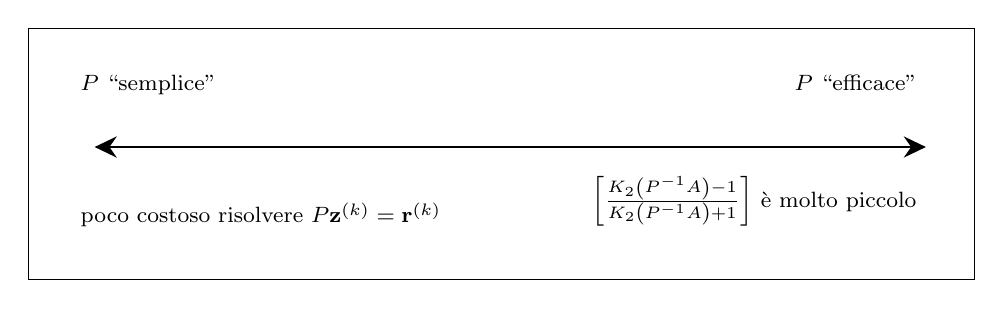
\begin{tikzpicture}[x=0.75pt,y=0.75pt,yscale=-1,xscale=1]
	%uncomment if require: \path (0,155); %set diagram left start at 0, and has height of 155

	%Straight Lines [id:da6554701139004233]
	\draw    (77,70) -- (471.5,70) ;
	\draw [shift={(474.5,70)}, rotate = 180] [fill={rgb, 255:red, 0; green, 0; blue, 0 }  ][line width=0.08]  [draw opacity=0] (10.72,-5.15) -- (0,0) -- (10.72,5.15) -- (7.12,0) -- cycle    ;
	\draw [shift={(74,70)}, rotate = 0] [fill={rgb, 255:red, 0; green, 0; blue, 0 }  ][line width=0.08]  [draw opacity=0] (10.72,-5.15) -- (0,0) -- (10.72,5.15) -- (7.12,0) -- cycle    ;
	%Shape: Rectangle [id:dp8278085571849905]
	\draw   (42,12.77) -- (497.81,12.77) -- (497.81,134) -- (42,134) -- cycle ;

	% Text Node
	\draw (66,34) node [anchor=north west][inner sep=0.75pt]  [font=\footnotesize] [align=left] {$P$ ``semplice''};
	% Text Node
	\draw (410,34) node [anchor=north west][inner sep=0.75pt]  [font=\footnotesize] [align=left] {$P$ ``efficace''};
	% Text Node
	\draw (66,95.5) node [anchor=north west][inner sep=0.75pt]  [font=\footnotesize] [align=left] {poco costoso risolvere $P\mathbf{z}^{(k)} =\mathbf{r}^{(k)}$};
	% Text Node
	\draw (312,83) node [anchor=north west][inner sep=0.75pt]  [font=\footnotesize] [align=left] {$\left[\frac{K_{2}\left( P^{-1} A\right) -1}{K_{2}\left( P^{-1} A\right) +1}\right]$ è molto piccolo};


	\end{tikzpicture}
\end{figure}
\FloatBarrier

\end{itemize}

\textbf{NB.}
Osserviamo che due vettori del residuo consecutivi nel metodo del gradiente non precondizionato (ma vale anche in quello precondizionato) soddisfano la seguente proprietà:
\begin{equation}
\left(\mathbf{r}^{( k+1)}\right)^{T}\mathbf{r}^{(k)} = 0,
\label{eq:prop-ortogonalita-gradiente}
\end{equation}
ovvero i valori del residuo sono \textit{a due a due ortogonali}. Quindi, ad ogni passo $k$ la nuova soluzione $\x^{( k+1)}$ è ottimale rispetto alla direzione di discesa $\mathbf{r}^{(k)}$.

\textit{Dimostrazione} di \eqref{eq:prop-ortogonalita-gradiente}. Ci ricordiamo la relazione di $\mathbf{r}^{( k+1)}$ che compare nell'algoritmo del gradiente e il valore di $\alpha _{k}$ \eqref{eq:alpha-ottimale-metodo-gradiente}:
\begin{equation*}
\mathbf{r}^{( k+1)} =\mathbf{r}^{(k)} -\alpha _{k} A\mathbf{r}^{(k)} ,\qquad \alpha _{k} =\frac{\left[\mathbf{r}^{(k)}\right]^{T}\mathbf{r}^{(k)}}{\left[\mathbf{r}^{(k)}\right]^{T} A\mathbf{r}^{(k)}} .
\end{equation*}
Calcoliamo il prodotto direttamente:
\begin{align*}
	\left(\mathbf{r}^{( k+1)}\right)^{T}\mathbf{r}^{(k)} & =\left(\mathbf{r}^{(k)} -\alpha _{k} A\mathbf{r}^{(k)}\right)^{T}\mathbf{r}^{(k)}                                                                                                                                         &                        \\
	                                                      & =\left(\left[\mathbf{r}^{(k)}\right]^{T} -\alpha _{k}\left[\mathbf{r}^{(k)}\right]^{T} A^{T}\right)\mathbf{r}^{(k)}                                                                                                       & \text{(trasposizione)} \\
	                                                      & =\left[\mathbf{r}^{(k)}\right]^{T}\mathbf{r}^{(k)} -\alpha _{k}\left[\mathbf{r}^{(k)}\right]^{T} A\mathbf{r}^{(k)}                                                                                                       & \text{(per simmetria)} \\
	                                                      & =\left[\mathbf{r}^{(k)}\right]^{T}\mathbf{r}^{(k)} -\frac{\left[\mathbf{r}^{(k)}\right]^{T}\mathbf{r}^{(k)}}{\left[\mathbf{r}^{(k)}\right]^{T} A\mathbf{r}^{(k)}}\left[\mathbf{r}^{(k)}\right]^{T} A\mathbf{r}^{(k)} & \text{(per ipotesi)}   \\
	                                                      & =\left[\mathbf{r}^{(k)}\right]^{T}\mathbf{r}^{(k)} -\left[\mathbf{r}^{(k)}\right]^{T}\mathbf{r}^{(k)}                                                                                                                    &                        \\
	                                                      & =0 \qed
\end{align*}

Notiamo tuttavia che \textit{non è garantito} che $\x^{( k+1)}$ sia ottimale rispetto a tutti i residui calcolati ai passi precedenti a $k$, ad esempio tutti i passi $j=0,\dotsc ,k-1$:
\begin{equation*}
\left[\mathbf{r}^{( k+1)}\right]^{T}\mathbf{r}^{(k)} =0,\quad\text{ma} \quad\left[\mathbf{r}^{( k+1)}\right]^{T}\mathbf{r}^{(j)} \neq 0,\quad j=0,\dotsc ,k-1.
\end{equation*}
Infatti, il metodo del gradiente non tiene traccia di tutte le direzioni precedenti, ma solo di quella immediatamente precedente.

\section{Metodo del gradiente coniugato}
\index{metodo!del gradiente coniugato}
È possibile modificare la direzione di discesa in modo da garantire un qualche criterio di \textit{ottimalità}?
Questa è l'idea che sta alla base del metodo del gradiente coniugato (GC o CG)\footnote{che ``è la Ferrari dei metodi iterativi''.}.
In particolare, dato un metodo iterativo
\begin{equation*}
\x^{( k+1)} =\x^{(k)} +\alpha _{k}\mathbf{p}^{(k)}
\end{equation*}
vogliamo scegliere direzioni di discesa che costituiscano una successione ottimale di vettori $\mathbf{p}^{(k)}$.
\begin{definition}
[Vettori $A$-coniugati]
Sia $A$ SDP fissata.
Due vettori $\mathbf{w} ,\mathbf{v} \in \mathbb{R}^{n}$ si dicono $A$-coniugati (o $A$-ortogonali) se
\begin{equation*}
\mathbf{w}^{T} A\ \mathbf{v} =0\quad\text{cioè} \quad ( A\mathbf{w})^{T}\mathbf{v} =0.
\end{equation*}
\end{definition}
\textit{Osservazioni.}
\begin{itemize}
\item Simmetria: $0=\left(\mathbf{w}^{T} A\ \mathbf{v}\right)^{T} =\mathbf{v}^{T} A^{T}\mathbf{w} =\mathbf{v}^{T} A\ \mathbf{w}$.
\item Annullamento: $\mathbf{v}^{T} A\mathbf{v} =0\ \Rightarrow \ \mathbf{v} =\mathbf{0}$.
\end{itemize}

\subsection{Scelta della direzione di discesa}
Scegliamo la seguente successione di vettori:
\begin{equation}
\begin{cases}
\mathbf{p}^{(0)} =\mathbf{r}^{(0)}\\
\mathbf{p}^{( k+1)} =\mathbf{r}^{( k+1)} -\beta _{k}\mathbf{p}^{(k)}
\end{cases} \quad \beta _{k} =\frac{\left( A\mathbf{p}^{(k)}\right)^{T}\mathbf{r}^{( k+1)}}{\left( A\mathbf{p}^{(k)}\right)^{T}\mathbf{p}^{(k)}} \quad k=0,1,2,\dotsc
\label{eq:scelta-metodo-cg}
\end{equation}
\textbf{Proprietà.}

Si può dimostrare per induzione che con la scelta \eqref{eq:scelta-metodo-cg} si ha:
\begin{enumerate}
\item $\left[\mathbf{p}^{(j)}\right]^{T}\mathbf{r}^{( k+1)} =0 \quad \forall j=0,1,\dotsc ,k$

La soluzione $\x^{( k+1)}$ è ottimale rispetto a \textit{tutte} le direzioni di discesa precedenti $\mathbf{p}^{(0)} ,\mathbf{p}^{(1)} ,\mathbf{p}^{(2)} ,\dotsc ,\mathbf{p}^{(k)}$.
\item $\left[ A\mathbf{p}^{(j)}\right]^{T}\mathbf{p}^{( k+1)} =0 \quad \forall j=0,1,\dotsc ,k$

La direzione di discesa $\mathbf{p}^{( k+1)}$ è $A$-ortogonale rispetto a \textit{tutte} le direzioni $\mathbf{p}^{(0)} ,\mathbf{p}^{(1)} ,\mathbf{p}^{(2)} ,\dotsc ,\mathbf{p}^{(k)}$. Ad ogni passo, l'algoritmo esplora e minimizza una direzione nuova, mai usata prima, tralasciando lo spazio già precedentemente esplorato.
\item Combinando $(1)$ e $(2)$ al passo $n$-esimo si ha $\mathbf{r}^{(n)} =0$, ossia $\x^{(n)}$ \textit{è la soluzione esatta}\footnote{Mai notizia più buona fu data.}.
\end{enumerate}

Dimostriamo la proprietà $(3)$, lasciando $(1)$ e $(2)$ al lettore come esercizio.
Per la proprietà $(1)$, al passo $k=n-1$ si ha:
\begin{equation*}
\underbrace{\mathbf{r}^{(n)}}_{\in \mathbb{R}^{n}} \perp \mathbf{p}^{(0)} ,\mathbf{p}^{(1)} ,\dotsc ,\mathbf{p}^{( n-1)}.
\end{equation*}
Non è ancora possibile concludere che $\mathbf{r}^{(n)}$ è nullo in quanto ortogonale ad altri $n$ vettori, perché non sappiamo se gli altri $\mathbf{p}^{(k)}$ sono indipendenti.
Ma vedremo che questa proprietà è assicurata dalla $(2)$.
Prendiamo la combinazione lineare dei vettori precedenti e poniamola uguale a $0$: vogliamo dimostrare che ciò implica necessariamente che tutti i coefficienti sono nulli:
\begin{equation*}
a_{0}\mathbf{p}^{(0)} +a_{1}\mathbf{p}^{(1)} +\dotsc +a_{n-1}\mathbf{p}^{( n-1)} =0\xrightarrow{\text{?}} a_{i} =0\quad\forall i=0,\dotsc ,n-1.
\end{equation*}
Moltiplichiamo a destra e sinistra per $\left( A\mathbf{p}^{(0)}\right)^{T}$:
\begin{equation*}
a_{0}\underbrace{\left( A\mathbf{p}^{(0)}\right)^{T}\mathbf{p}^{(0)}}_{ >0\text{ se }\mathbf{p}^{(0)} \neq 0} +a_{1}\underbrace{\left( A\mathbf{p}^{(0)}\right)^{T}\mathbf{p}^{(1)}}_{=0\ \text{per} \ (2)} +\dotsc +a_{n-1}\left( A\mathbf{p}^{(0)}\right)^{T}\mathbf{p}^{( n-1)} =0 \ \ \Rightarrow \ \ a_{0} =0.
\end{equation*}
Analogamente moltiplicando per $\left( A\mathbf{p}^{(1)}\right)^{T}$ si ricava $a_{1} =0$ e così via. Infine si ottiene $a_{i} =0\ \ \forall i$, ovvero che tutti i $\mathbf{p}^{(i)}$ sono linearmente indipendenti. \textqed

\subsection{Scelta del parametro di accelerazione}
Ripercorrendo gli stessi passi della sezione \eqref{sez:metodo-del-gradiente} sulla minimizzazione del funzionale $\Phi ( \cdot )$, valutato questa volta in $\x^{( k+1)} =\x^{(k)} +\alpha _{k}\mathbf{p}^{(k)}$, troviamo:
\begin{equation*}
\alpha_{k} =\frac{\left[\mathbf{p}^{(k)}\right]^{T}\mathbf{r}^{(k)}}{\left[\mathbf{p}^{(k)}\right]^{T} A\ \mathbf{p}^{(k)}}.
\end{equation*}
Riassumiamo il gradiente coniugato in pseudocodice: \\
\begin{algo}
	inizializza $\x^{(0)}$\;
	calcola $\mathbf{r}^{(0)} =\mathbf{b} -A\x^{(0)}$\;
	inizializza $\mathbf{p}^{(0)} =\mathbf{r}^{(0)}$\;
	\For{$k=0,1,2,\dotsc $}{
		calcola il parametro $\alpha _{k} =\frac{\left[\mathbf{p}^{(k)}\right]^{T}\mathbf{r}^{(k)}}{\left[\mathbf{p}^{(k)}\right]^{T} A\ \mathbf{p}^{(k)}}$\;
		aggiorna $\x^{( k+1)} =\x^{(k)} +\alpha _{k}\mathbf{p}^{(k)}$\;
		aggiorna $\mathbf{r}^{( k+1)} =\mathbf{r}^{(k)} -\alpha _{k} A\mathbf{p}^{(k)}$\;
		calcola il parametro $\beta _{k} =\frac{\left( A\mathbf{p}^{(k)}\right)^{T}\mathbf{r}^{( k+1)}}{\left( A\mathbf{p}^{(k)}\right)^{T}\mathbf{p}^{(k)}}$\;
		aggiorna $\mathbf{p}^{( k+1)} =\mathbf{r}^{( k+1)} -\beta _{k}\mathbf{p}^{(k)}$\;
		\If{criterio di arresto}{
			termina algoritmo\;
		}
	}
	\caption{Algoritmo del metodo del gradiente coniugato, non precondizionato}
\end{algo}
\index{algoritmo!gradiente coniugato}
\begin{theorem}
[Convergenza del metodo GC]
Sia $A$ una matrice SDP in aritmetica esatta.
Allora il metodo GC converge alla soluzione esatta di $A \x = \mathbf b$ in al più $n$ passi. Inoltre, per ogni iterazione $k=0,\dotsc ,n$, l'errore $\mathbf{e}^{(k)}$ è ortogonale alla direzione $\mathbf{p}^{(j)} \quad j=0,\dotsc ,k-1$ e
\begin{equation*}
\left\Vert \mathbf{e}^{(k)}\right\Vert _{A} \leqslant \left[\frac{2c^{k}}{1+c^{2k}}\right]\left\Vert \mathbf{e}^{(0)}\right\Vert _{A} \quad\text{con} \quad c=\frac{\sqrt{K_{2}(A)} -1}{\sqrt{K_{2}(A)} +1}.
\end{equation*}
\label{thm:convergenza-metodo-cg}
\end{theorem}
\textit{Osservazioni.}
\begin{itemize}
\item Se $A$ è SDP, allora $K_{2}(A) =\frac{\lambda _{\text{max}}(A)}{\lambda _{\text{min}}(A)}$.
%\item In aritmetica esatta abbiamo la certezza che l'algoritmo termini dopo al più $n$ passi restituendo la soluzione esatta. % l'hai già detto
\item Come per il metodo del gradiente la convergenza è monotona, e in particolare la sua velocità dipende da $\sqrt{K_{2}(A)}$.
\end{itemize}

Scriviamo ora la versione precondizionata del gradiente coniugato: \\
\begin{algo}
	inizializza $\x^{(0)}$\;
	calcola $\mathbf{r}^{(0)} =\mathbf{b} -A\x^{(0)}$\;
	risolvi $P\mathbf{z}^{(0)} = \mathbf{r}^{(0)}$\;
	inizializza $\mathbf{p}^{(0)} = \mathbf{z}^{(0)}$\;
	\For{$k=0,1,2,\dotsc$}{
		calcola il parametro $\alpha _{k} =\frac{\left[\mathbf{p}^{(k)}\right]^{T}\mathbf{r}^{(k)}}{\left[\mathbf{p}^{(k)}\right]^{T} A\ \mathbf{p}^{(k)}}$\;
		aggiorna $\x^{( k+1)} =\x^{(k)} +\alpha _{k}\mathbf{p}^{(k)}$\;
		aggiorna $\mathbf{r}^{( k+1)} =\mathbf{r}^{(k)} -\alpha _{k} A\mathbf{p}^{(k)}$\;
		risolvi $P\mathbf{z}^{(k+1)} = \mathbf{r}^{(k+1)}$\;
		calcola il parametro $\beta _{k} =\frac{\left( A\mathbf{p}^{(k)}\right)^{T}\mathbf{z}^{(k+1)}}{\left( A\mathbf{p}^{(k)}\right)^{T}\mathbf{p}^{(k)}}$\;
		aggiorna $\mathbf{p}^{( k+1)} =\mathbf{z}^{(k+1)} -\beta _{k}\mathbf{p}^{(k)}$\;
		\If{criterio di arresto}{
			termina algoritmo\;
		}
	}
	\caption{Algoritmo del metodo del gradiente coniugato, precondizionato}
\end{algo}
\index{algoritmo!gradiente coniugato}
Per esso vale lo stesso teorema di convergenza \ref{thm:convergenza-metodo-cg}, con
\begin{equation*}
c=\frac{\sqrt{K_{2}\left( P^{-1} A\right)} -1}{\sqrt{K_{2}\left( P^{-1} A\right)} +1}.
\end{equation*}
\section{Criteri di arresto}

I criteri di arresto non dipendono nello specifico dai metodi che stiamo utilizzando. Fissiamo una tolleranza $\operatorname{TOL}$, ovvero una quantità decisa dall'utente, che la sceglie in base a quanta precisione desidera nel calcolo della soluzione.
%$Non è necessariamente il più piccolo numero del calcolatore (potremmo aver bisogno di tolleranza $10^{-6}$ e non $10^{-16}$). % bah
Più piccola è $\operatorname{TOL}$, più iterazioni l'algoritmo necessita per convergere: dobbiamo trovare un equilibrio, un trade-off, tra quanto vogliamo essere accurati e quante iterazioni siamo disposti ad aspettare.
\begin{enumerate}
\item \textbf{Criterio sul residuo.} Arrestiamo il ciclo quando
\begin{equation*}
\frac{\left\Vert \mathbf{r}^{( k+1)}\right\Vert }{\Vert \mathbf{b}\Vert } \leqslant \operatorname{TOL}.
\end{equation*}
\item \textbf{Criterio sull'incremento.} Arrestiamo il ciclo quando
\begin{equation*}
\left\Vert \x^{( k+1)} -\x^{(k)}\right\Vert \leqslant \operatorname{TOL}.
\end{equation*}
\item \textbf{Criterio di controllo.} Arrestiamo il ciclo dopo $n_{\text{max}}$ iterazioni.
\end{enumerate}

\textit{Osservazioni.}
\begin{itemize}
\item I criteri (1) e (2) agiscono in funzione della \textit{qualità della soluzione}, mentre (3) è un criterio di emergenza.
\item Di norma si sceglie di usare uno tra i primi due criteri, abbinati sempre al terzo. Infatti ci sono matrici che convergono lentissimamente, che hanno bisogno di molte iterazioni per raggiungere un risultato soddisfacente.
\item Ogni iterazione di Gauss-Seidel costa $n^{2}$ operazioni. Dopo $n$ iterazioni, il costo complessivo diventa $n^{3}$, esattamente il costo di una fattorizzazione con metodo diretto. Per tutti i problemi in cui non c'è problema di memoria limitata e quindi possiamo scegliere fra metodi diretti e iterativi, il metodo iterativo è molto più conveniente nella misura in cui andiamo a usare un criterio di arresto in meno di $n$ operazioni. Quindi $n_{\text{max}} \approx n$. Se abbiamo troppo poco spazio, i metodi iterativi sono d'obbligo.
\item Il criterio (2) lascia proseguire l'algoritmo fintanto che fra l'iterazione $(k)$ e l'iterazione $( k+1)$ c'è sufficiente progresso. Se $\x^{(k)}$ e $\x^{( k+1)}$ sono molto vicine, significa che l'algoritmo sta stagnando.
\item Un criterio si dice \textbf{affidabile} se nel momento in cui si verifica la condizione, abbiamo la garanzia che anche l'errore (normalizzato) sia minore della tolleranza moltiplicata per una costante.
\end{itemize}
\subsection{Criterio sul residuo}

Controlliamo l'affidabilità del criterio sul residuo. L'algoritmo si arresta quando si verifica:
\begin{equation}
\frac{\left\Vert \mathbf{r}^{(k)}\right\Vert }{\Vert \mathbf{b}\Vert } \leqslant \operatorname{TOL}.
\label{eq:criterio-residuo}
\end{equation}
Dobbiamo verificare se valga la seguente implicazione, come notato nelle osservazioni:
\begin{equation*}
\frac{\left\Vert \mathbf{r}^{(k)}\right\Vert }{\Vert \mathbf{b}\Vert } \leqslant \operatorname{TOL} \ \ \overset{?}{\Rightarrow } \ \ \frac{\left\Vert \mathbf{e}^{(k)}\right\Vert }{\Vert \x\Vert } =\frac{\left\Vert \x -\x^{(k)}\right\Vert }{\Vert \x\Vert } \leqslant C\ \operatorname{TOL}.
\end{equation*}
A tal proposito, ricordiamo il teorema di stabilità dei sistemi lineari \ref{thm:teorema-di-stabilita}:
\begin{equation*}
\frac{\left\Vert \x -\tilde{\x}\right\Vert }{\Vert \x\Vert } \leqslant K_{2}(A)\frac{\left\Vert \mathbf{b} -A\tilde{\x}\right\Vert }{\Vert \mathbf{b}\Vert }
\end{equation*}
Prendendo $\tilde{\x} =\x^{(k)}$ e ricordando che $\mathbf{b} -A\x^{(k)} =\mathbf{r}^{(k)}$, l'enunciato del teorema diventa:
\begin{equation}
\frac{\left\Vert \x -\x^{(k)}\right\Vert }{\Vert \x\Vert } \leqslant K_{2}(A)\frac{\left\Vert \mathbf{r}^{(k)} \ \right\Vert }{\Vert \mathbf{b}\Vert } \leqslant K_{2}(A) \ \operatorname{TOL}.
\label{eq:criterio-residuo2}
\end{equation}
Quindi il criterio d'arresto sul residuo \eqref{eq:criterio-residuo} è affidabile solo se la matrice è ben condizionata. Nel caso usassimo un precondizionatore, bisogna sostituire il criterio con il seguente:
\begin{equation*}
\frac{\left\Vert P^{-1}\mathbf{r}^{(k)}\right\Vert }{\left\Vert P^{-1}\mathbf{r}^{(0)}\right\Vert } \leqslant \operatorname{TOL} \quad \text{oppure analogamente} \quad \frac{\left\Vert \mathbf{z}^{(k)}\right\Vert }{\left\Vert \mathbf{z}^{(0)}\right\Vert } \leqslant \operatorname{TOL},
\end{equation*}
in tal caso la \eqref{eq:criterio-residuo2} diventa:
\begin{equation*}
\frac{\left\Vert \x -\x^{(k)}\right\Vert }{\Vert \x\Vert } \leqslant K_{2}\left( P^{-1} A\right) \ \operatorname{TOL}.
\end{equation*}
\subsection{Criterio sull'incremento}

Studiamo ora l'affidabilità del criterio sull'incremento:
\begin{equation}
\frac{\left\Vert \x^{( k+1)} -\x^{(k)}\right\Vert }{\left\Vert \x^{( k+1)}\right\Vert } \leqslant \operatorname{TOL}.
\label{eq:criterio-incremento}
\end{equation}
Bisogna verificare la seguente implicazione:
\begin{equation*}
\frac{\left\Vert \x^{( k+1)} -\x^{(k)}\right\Vert }{\left\Vert \x^{( k+1)}\right\Vert } \leqslant \operatorname{TOL} \ \ \overset{?}{\Rightarrow } \ \ \frac{\left\Vert \mathbf{e}^{(k)}\right\Vert }{\Vert \x\Vert } =\frac{\left\Vert \x -\x^{(k)}\right\Vert }{\Vert \x\Vert } \leqslant C\ \operatorname{TOL}.
\end{equation*}
A tal proposito, ricordiamo:
\begin{align*}
\x^{( k+1)} & =B\x^{(k)} +\mathbf{g} & \text{(forma generale)}\\
\x & =B\x +\mathbf{g} & \text{(consistenza)}\\
\x^{( k+1)} -\x & =B(\x^{(k)} -\x). & \text{(differenza)}
\end{align*}
L'errore $k$-esimo si può scrivere come:
\begin{align*}
  \left\Vert \mathbf{e}^{(k)}\right\Vert =\left\Vert \x^{(k)} -\x\right\Vert & =\left\Vert \x^{(k)} -\x^{( k+1)} +\x^{( k+1)} -\x\right\Vert                                             &                           \\
  & \leqslant \left\Vert \x^{( k+1)} -\x^{(k)}\right\Vert +\left\Vert \x^{( k+1)} -\x\right\Vert              & \text{(dis. triangolare)} \\
  & \leqslant \left\Vert \x^{( k+1)} -\x^{(k)}\right\Vert +\Vert B\Vert \ \left\Vert \x^{(k)} -\x\right\Vert. & \text{(per quanto detto)}
\end{align*}
Portiamo a sinistra e dividiamo per $1-\Vert B\Vert $:
\begin{align*}
( 1-\Vert B\Vert )\left\Vert \x^{(k)} -\x\right\Vert  & \leqslant \left\Vert \x^{( k+1)} -\x^{(k)}\right\Vert \\
\underbrace{\left\Vert \x^{(k)} -\x\right\Vert }_{\left\Vert \mathbf{e}^{(k)}\right\Vert } & \leqslant \frac{1}{1-\Vert B\Vert }\left\Vert \x^{( k+1)} -\x^{(k)}\right\Vert.
\end{align*}
Infine, ricordando la formula di rappresentazione dell'errore $\mathbf{e}^{( k+1)} =B\mathbf{e}^{(k)}$:
\begin{align*}
\left\Vert \x^{( k+1)} -\x\right\Vert  & =\left\Vert \mathbf{e}^{( k+1)}\right\Vert  & \\
 & =\left\Vert B\mathbf{e}^{(k)}\right\Vert  & \text{(formula di rappr. dell'errore)}\\
 & \leqslant \Vert B\Vert \ \left\Vert \mathbf{e}^{(k)}\right\Vert  & \text{(proprietà della norma)}\\
 & \leqslant \frac{\Vert B\Vert }{1-\Vert B\Vert }\left\Vert \x^{( k+1)} -\x^{(k)}\right\Vert.  & \text{(per quanto appena trovato)}
\end{align*}
Otteniamo infine:
\begin{equation}
\left\Vert \x -\x^{( k+1)}\right\Vert \leqslant \frac{\Vert B\Vert }{1-\Vert B\Vert } \ \left\Vert \x^{( k+1)} -\x^{(k)}\right\Vert.
\label{eq:criterio-incremento2}
\end{equation}

Poiché il metodo è convergente si ha $\rho (B) < 1$, quindi $\Vert B\Vert < 1$. Il criterio è quindi affidabile. La \eqref{eq:criterio-incremento2} si può anche riscrivere come
\begin{equation*}
\left\Vert \x -\x^{( k+1)}\right\Vert \leqslant \left[\frac{1}{1-\rho (B)}\right]\left\Vert \x^{( k+1)} -\x^{(k)}\right\Vert.
\end{equation*}
Quindi se $\Vert B\Vert $ è molto vicina a $1$, cioè se $A$ è mal condizionata, la differenza tra l'errore vero e quello che sappiamo misurare diventa molto grande e quindi dà poche informazioni.

%!TEX root = ../main.tex
% \textit{[Lezione 10 (02-04-2020)]}

\chapter{Approssimazione di funzioni e dati}

L'obiettivo di un'approssimazione funzionale è sostituire una funzione \textit{complicata} con una funzione \textit{semplice} ricercata in una classe prefissata di funzioni, in genere dei polinomi.

\textit{Esempio.} L'espressione analitica di una funzione $f$ non è nota, ma essa è solo campionata, ovvero il suo valore è noto solamente su un insieme di punti $x_0, \dots, x_n$, e vogliamo determinare una possibile espressione di $f$.

\begin{figure}[htpb]
	\centering
	\tikzset{every picture/.style={line width=0.75pt}} %set default line width to 0.75pt

	\begin{tikzpicture}[x=0.75pt,y=0.75pt,yscale=-1,xscale=1]
	%uncomment if require: \path (0,216); %set diagram left start at 0, and has height of 216

	%Shape: Axis 2D [id:dp7681657976935359]
	\draw  (234,173.52) -- (508.5,173.52)(261.45,36.17) -- (261.45,188.78) (501.5,168.52) -- (508.5,173.52) -- (501.5,178.52) (256.45,43.17) -- (261.45,36.17) -- (266.45,43.17)  ;
	%Curve Lines [id:da48740805964175427]
	\draw  [dash pattern={on 0.84pt off 2.51pt}]  (245.5,144.78) .. controls (312,51.17) and (432,179.17) .. (489,58.17) ;
	%Straight Lines [id:da43786339887025716]
	\draw    (293,168.59) -- (293,178) ;
	%Straight Lines [id:da023194448258216926]
	\draw    (333,168.59) -- (333,178) ;
	%Straight Lines [id:da8232346787407612]
	\draw    (373,168.59) -- (373,178) ;
	%Straight Lines [id:da4457891900858195]
	\draw    (473,168.59) -- (473,178) ;
	%Shape: Circle [id:dp24863242874775415]
	\draw  [draw opacity=0][fill={rgb, 255:red, 0; green, 0; blue, 0 }  ,fill opacity=1 ] (291,110.59) .. controls (291,109.49) and (291.9,108.59) .. (293,108.59) .. controls (294.1,108.59) and (295,109.49) .. (295,110.59) .. controls (295,111.7) and (294.1,112.59) .. (293,112.59) .. controls (291.9,112.59) and (291,111.7) .. (291,110.59) -- cycle ;
	%Shape: Circle [id:dp914917520550603]
	\draw  [draw opacity=0][fill={rgb, 255:red, 0; green, 0; blue, 0 }  ,fill opacity=1 ] (331,107.59) .. controls (331,106.49) and (331.9,105.59) .. (333,105.59) .. controls (334.1,105.59) and (335,106.49) .. (335,107.59) .. controls (335,108.7) and (334.1,109.59) .. (333,109.59) .. controls (331.9,109.59) and (331,108.7) .. (331,107.59) -- cycle ;
	%Shape: Circle [id:dp6230329978907112]
	\draw  [draw opacity=0][fill={rgb, 255:red, 0; green, 0; blue, 0 }  ,fill opacity=1 ] (371,112.59) .. controls (371,111.49) and (371.9,110.59) .. (373,110.59) .. controls (374.1,110.59) and (375,111.49) .. (375,112.59) .. controls (375,113.7) and (374.1,114.59) .. (373,114.59) .. controls (371.9,114.59) and (371,113.7) .. (371,112.59) -- cycle ;
	%Shape: Circle [id:dp7316490236444106]
	\draw  [draw opacity=0][fill={rgb, 255:red, 0; green, 0; blue, 0 }  ,fill opacity=1 ] (471,83.59) .. controls (471,82.49) and (471.9,81.59) .. (473,81.59) .. controls (474.1,81.59) and (475,82.49) .. (475,83.59) .. controls (475,84.7) and (474.1,85.59) .. (473,85.59) .. controls (471.9,85.59) and (471,84.7) .. (471,83.59) -- cycle ;

	% Text Node
	\draw (244,16.4) node [anchor=north west][inner sep=0.75pt]    {$y$};
	% Text Node
	\draw (523,166.4) node [anchor=north west][inner sep=0.75pt]    {$x$};
	% Text Node
	\draw (285,180.4) node [anchor=north west][inner sep=0.75pt]    {$x_{0}$};
	% Text Node
	\draw (325,180.4) node [anchor=north west][inner sep=0.75pt]    {$x_{1}$};
	% Text Node
	\draw (365,180.4) node [anchor=north west][inner sep=0.75pt]    {$x_{2}$};
	% Text Node
	\draw (465,180.4) node [anchor=north west][inner sep=0.75pt]    {$x_{n}$};
	% Text Node
	\draw (75,60.4) node [anchor=north west][inner sep=0.75pt]    {$\begin{array}{ c|c }
	x & f( x)\\
	\hline
	x_{0} & y_{0} =f( x_{0})\\
	x_{1} & y_{1} =f( x_{1})\\
	\vdots  & \vdots \\
	x_{n} & y_{n} =f( x_{n})
	\end{array}$};
	% Text Node
	\draw (413,179.4) node [anchor=north west][inner sep=0.75pt]    {$\dotsc $};


	\end{tikzpicture}
	\caption{Esempio monodimensionale in cui conosciamo il valore della funzione, solo in alcuni punti, ma vogliamo in qualche modo determinarne un'approssimazione. La linea tratteggiata indica una delle tante possibilità di $f$, infatti passa per tutti i campionamenti.}
	\label{fig:esempio-campionamento}
\end{figure}
\FloatBarrier

\textit{Esempio.} Conosciamo l'espressione analitica di $f$, ma vogliamo sostituirla con una funzione più \textit{semplice} per il calcolo numerico oppure, ad esempio, per rendere possibili o più semplici delle operazioni funzionali quali l'integrazione o la derivazione.

% Pattern Info

\begin{figure}[htpb]
	\centering
	\tikzset{
	pattern size/.store in=\mcSize,
	pattern size = 5pt,
	pattern thickness/.store in=\mcThickness,
	pattern thickness = 0.3pt,
	pattern radius/.store in=\mcRadius,
	pattern radius = 1pt}
	\makeatletter
	\pgfutil@ifundefined{pgf@pattern@name@_5a3929o9p}{
	\pgfdeclarepatternformonly[\mcThickness,\mcSize]{_5a3929o9p}
	{\pgfqpoint{0pt}{-\mcThickness}}
	{\pgfpoint{\mcSize}{\mcSize}}
	{\pgfpoint{\mcSize}{\mcSize}}
	{
	\pgfsetcolor{\tikz@pattern@color}
	\pgfsetlinewidth{\mcThickness}
	\pgfpathmoveto{\pgfqpoint{0pt}{\mcSize}}
	\pgfpathlineto{\pgfpoint{\mcSize+\mcThickness}{-\mcThickness}}
	\pgfusepath{stroke}
	}}
	\makeatother
	\tikzset{every picture/.style={line width=0.75pt}} %set default line width to 0.75pt

	\begin{tikzpicture}[x=0.75pt,y=0.75pt,yscale=-1,xscale=1]
	%uncomment if require: \path (0,198); %set diagram left start at 0, and has height of 198

	%Shape: Axis 2D [id:dp63552661394887]
	\draw  (77.5,171.14) -- (378.5,171.14)(107.6,21.33) -- (107.6,187.78) (371.5,166.14) -- (378.5,171.14) -- (371.5,176.14) (102.6,28.33) -- (107.6,21.33) -- (112.6,28.33)  ;
	%Shape: Polygon Curved [id:ds9891591629339485]
	\draw  [pattern=_5a3929o9p,pattern size=3.75pt,pattern thickness=0.75pt,pattern radius=0pt, pattern color={rgb, 255:red, 155; green, 155; blue, 155}] (157.6,91.18) .. controls (208.5,50.78) and (266.5,151.78) .. (347.6,51.18) .. controls (347.75,114.25) and (348.25,134.75) .. (347.6,171.18) .. controls (292.75,170.75) and (218.75,171.75) .. (157.6,171.18) .. controls (158.25,144.25) and (157.25,131.25) .. (157.6,91.18) -- cycle ;
	%Straight Lines [id:da8306255568313834]
	\draw    (257.33,96.78) -- (257.33,174.33) ;
	%Shape: Boxed Line [id:dp24784071198944235]
	\draw    (391.29,116) -- (128,78) ;

	% Text Node
	\draw (87.33,12.07) node [anchor=north west][inner sep=0.75pt]    {$y$};
	% Text Node
	\draw (387,161.73) node [anchor=north west][inner sep=0.75pt]    {$x$};
	% Text Node
	\draw (329.33,25.73) node [anchor=north west][inner sep=0.75pt]    {$f(x)$};
	% Text Node
	\draw (150.33,173.73) node [anchor=north west][inner sep=0.75pt]    {$a$};
	% Text Node
	\draw (250.33,173.73) node [anchor=north west][inner sep=0.75pt]    {$\overline{x}$};
	% Text Node
	\draw (342.33,173.73) node [anchor=north west][inner sep=0.75pt]    {$b$};
	% Text Node
	\draw (399.33,35.73) node [anchor=north west][inner sep=0.75pt]    {$\int\limits ^{b}_{a} f(x) \dx\approx \int\limits ^{b}_{a} f_{n}(x) \dx$};
	% Text Node
	\draw (399.33,103.73) node [anchor=north west][inner sep=0.75pt]    {$f'(\overline{x}) \approx f'_{n}(x)$};


	\end{tikzpicture}
	\caption{Cercheremo di approssimare anche le derivate di una funzione e gli integrali definiti in base ai campionamenti della funzione stessa (ovviamente non si può \textit{campionare la derivata o l'integrale}).}
\end{figure}
\FloatBarrier
Nel contesto delle equazioni differenziali è fondamentale saper approssimare funzioni e dati.

\section{Polinomio di interpolazione di Lagrange}
Siano assegnate $( n+1)$ coppie, $n\geqslant 0$, di punti \textit{distinti} nel piano, come in figura \ref{fig:esempio-campionamento}.

Vogliamo costruire un polinomio $\Pi _{n}(x) \in \mathbb{P}^{n}$ di grado $n$ tale che
\begin{equation*}
\Pi _{n}( x_{i}) =y_{i} \quad\forall i=0,1,\dotsc ,n.
\end{equation*}
Questa procedura è definita \textbf{interpolazione}\index{interpolazione}.

\textit{Osservazione.} Se al posto di avere i soli punti di campionamento $( x_{i} ,y_{i}), i=0,\dotsc ,n$ avessimo una funzione complicata che vogliamo approssimare, allora l'insieme di condizioni da imporre è dato da
\begin{equation*}
( x_{i} ,f( x_{i})) \quad i=0,\dotsc ,n
\end{equation*}
e le condizioni diventano
\begin{equation*}
\Pi _{n} f(x_{i}) =f( x_{i}) \quad\forall i=0,\dotsc ,n.
\end{equation*}
\begin{figure}[htpb]
	\centering
	\tikzset{every picture/.style={line width=0.75pt}} %set default line width to 0.75pt

	\begin{tikzpicture}[x=0.75pt,y=0.75pt,yscale=-1,xscale=1]
	%uncomment if require: \path (0,180); %set diagram left start at 0, and has height of 180

	%Shape: Axis 2D [id:dp22400730037348748]
	\draw  (168,148.78) -- (441.5,148.78)(168,31.23) -- (168,148.78) -- cycle (434.5,143.78) -- (441.5,148.78) -- (434.5,153.78) (163,38.23) -- (168,31.23) -- (173,38.23)  ;
	%Curve Lines [id:da32352899128716883]
	\draw  [dash pattern={on 0.84pt off 2.51pt}]  (202.5,128.78) .. controls (269.5,13.78) and (322.5,184.78) .. (416.5,41.78) ;
	%Straight Lines [id:da839820950039138]
	\draw    (230.33,143.67) -- (230.33,152.33) ;
	%Straight Lines [id:da7873722676835229]
	\draw    (280.33,143.67) -- (280.33,152.33) ;
	%Straight Lines [id:da8564842660802718]
	\draw    (390.33,143.67) -- (390.33,152.33) ;
	%Shape: Circle [id:dp6129946178962862]
	\draw  [fill={rgb, 255:red, 0; green, 0; blue, 0 }  ,fill opacity=1 ] (228.17,96.51) .. controls (228.17,95.4) and (229.06,94.51) .. (230.17,94.51) .. controls (231.27,94.51) and (232.17,95.4) .. (232.17,96.51) .. controls (232.17,97.61) and (231.27,98.51) .. (230.17,98.51) .. controls (229.06,98.51) and (228.17,97.61) .. (228.17,96.51) -- cycle ;
	%Shape: Circle [id:dp25002038836612006]
	\draw  [fill={rgb, 255:red, 0; green, 0; blue, 0 }  ,fill opacity=1 ] (277.17,89.51) .. controls (277.17,88.4) and (278.06,87.51) .. (279.17,87.51) .. controls (280.27,87.51) and (281.17,88.4) .. (281.17,89.51) .. controls (281.17,90.61) and (280.27,91.51) .. (279.17,91.51) .. controls (278.06,91.51) and (277.17,90.61) .. (277.17,89.51) -- cycle ;
	%Shape: Circle [id:dp7481993899672381]
	\draw  [fill={rgb, 255:red, 0; green, 0; blue, 0 }  ,fill opacity=1 ] (388.37,74.31) .. controls (388.37,73.2) and (389.26,72.31) .. (390.37,72.31) .. controls (391.47,72.31) and (392.37,73.2) .. (392.37,74.31) .. controls (392.37,75.41) and (391.47,76.31) .. (390.37,76.31) .. controls (389.26,76.31) and (388.37,75.41) .. (388.37,74.31) -- cycle ;
	%Curve Lines [id:da6764086869694204]
	\draw    (205.6,135.8) .. controls (212.4,124.2) and (220.4,112.2) .. (230.33,96.67) .. controls (239.6,84.6) and (249.87,65.94) .. (280.33,90.67) .. controls (310.8,115.4) and (366.27,125.14) .. (390.33,74.67) .. controls (401.2,50.2) and (405.6,42.6) .. (411.6,29) ;

	% Text Node
	\draw (147,26.4) node [anchor=north west][inner sep=0.75pt]    {$y$};
	% Text Node
	\draw (453,136.4) node [anchor=north west][inner sep=0.75pt]    {$x$};
	% Text Node
	\draw (223,152.4) node [anchor=north west][inner sep=0.75pt]    {$x_{0}$};
	% Text Node
	\draw (273,152.4) node [anchor=north west][inner sep=0.75pt]    {$x_{1}$};
	% Text Node
	\draw (383,152.4) node [anchor=north west][inner sep=0.75pt]    {$x_{n}$};
	\end{tikzpicture}
	\caption{Esistono diverse possibilità che rispettano le condizioni di passaggio nei nodi, è importante formalizzare delle strategie e dei criteri per determinare la migliore interpolazione.}
\end{figure}
\FloatBarrier

\begin{theorem}
Dati $n+1$ punti distinti $x_{0} ,x_{1} ,\dotsc ,x_{n}$, detti nodi di interpolazione, e $n+1$ corrispondenti valori $y_{0} ,y_{1} ,\dotsc ,y_{n}$, allora esiste un unico polinomio di interpolazione $\Pi _{n}(x)$ di grado $n$ tale che
\begin{equation}
\Pi _{n}( x_{i}) =y_{i} \quad \forall i=0,\dotsc ,n.
\label{eq:condizione-pol-interpolazione}
\end{equation}
\end{theorem}
\textbf{NB.}
Per giustificare intuitivamente il fatto che servano $n+1$ punti, ricordiamo che esiste una e una sola retta (polinomio di grado 1) passante per due punti, mentre esistono infinite parabole (polinomio di grado 2) passanti per due punti. Pertanto per fissare il nostro oggetto di grado $n$ ci servono $n+1$ punti.

\textit{Dimostrazione.} La dimostrazione è costruttiva, ovvero contiene il modo operativo per calcolare il polinomio di interpolazione. Dobbiamo mostrare che questo esista e che sia unico.

\textit{Esistenza.} Forniamo una rappresentazione esplicita del polinomio $\Pi _{n}$. Abbiamo bisogno di costruire una base per lo spazio dei polinomi di grado $n\rightarrow \mathbb{P}^{n}$ definiti su $\mathbb{R}$. Una scelta molto semplice è utilizzare la base dei monomi
\begin{equation*}
\mathbb{P}^{n} =\operatorname{span}\left\{1,x,x^{2} ,\dotsc ,x^{n}\right\} ,
\end{equation*}
cioè scrivere $\Pi _{n}(x)$ come
\begin{equation*}
\Pi _{n}(x) =a_{0} +a_{1} x+a_{2} x^{2} +\dotsc +a_{n} x^{n} ,
\end{equation*}
con $a_{0} ,a_{1} ,\dotsc ,a_{n} \in \mathbb{R}$ da determinare imponendo i vincoli di passaggio \eqref{eq:condizione-pol-interpolazione}. Costruiamo quindi una nuova base, detta \textbf{base di Lagrange}\index{base!di Lagrange}:
\begin{equation*}
\mathbb{P}^{n} =\operatorname{span}\{\mathcal{L}_{0}(x) ,\dotsc ,\mathcal{L}_{n}(x)\}
\end{equation*}
dove per ogni $i=0,\dotsc ,n$ l'$i$-esimo \textbf{polinomio di Lagrange}\index{polinomio!di Lagrange} $\mathcal{L}_{i}(x)$ è definito in modo da soddisfare le seguenti condizioni:
\begin{equation*}
\begin{array}{{>{\displaystyle}l}}
\mathcal{L}_{i}(x) \ \text{è un polinomio di grado} \ n\\
\mathcal{L}_{i}(x) =\begin{cases}
1 & \text{se} \ x=x_{i}\\
0 & \text{se} \ x=x_{j} ,\ j\neq i.
\end{cases}
\end{array}
\end{equation*}
L'espressione analitica di ogni $\mathcal{L}_{i}(x) ,i=0,\dotsc ,n$ è:
\begin{equation*}
\mathcal{L}_{i}(x) =\prod ^{n}_{j=0,j\neq i}\frac{( x-x_{j})}{( x_{i} -x_{j})} \quad i=0,\dotsc ,n,
\end{equation*}
in quanto il numeratore si annulla in ogni $x_j$ con $j\ne i$, mentre il denominatore coincide con il numeratore calcolato in $x_i$.

In figura \ref{fig-polinomi-lagrange} si può vedere un esempio di un set di polinomi di Lagrange costruiti su un specifico insieme di nodi.
\fg[Polinomi di Lagrange nei nodi $x_{i}=1,3,4,6,8$.]{0.75}{fig-polinomi-lagrange}

Si può dimostrare che questi polinomi sono indipendenti e che quindi costituiscono una base per i polinomi $\mathbb{P}^{n}$. Con questa base è immediato costruire il polinomio di interpolazione $\Pi _{n}(x)$, infatti:
\begin{equation*}
\Pi _{n}(x) =y_{0}\mathcal{L}_{0}(x) +y_{1}\mathcal{L}_{1}(x) +\dotsc +y_{n}\mathcal{L}_{n}(x).
\end{equation*}
Ovvero in forma compatta otteniamo:
\begin{equation*}
\Pi _{n}(x) =\sum ^{n}_{i=0} y_{i}\mathcal{L}_{i}(x) .
\end{equation*}
Questo ne dimostra l'esistenza.

\textit{Unicità.} Per assurdo supponiamo che esistano due polinomi di grado $n$ distinti $\Pi _{n}(x)$ e $\tilde{\Pi }_{n}(x)$ che rispettino le proprietà richieste, ovvero:
\begin{equation*}
\Pi _{n}( x_{i}) =y_{i} \quad \forall i=0,\dotsc ,n \quad \text{e} \quad \tilde{\Pi }_{n}( x_{i}) =y_{i} \quad \forall i=0,\dotsc ,n.
\end{equation*}
Definiamo ora $\mathcal{Y}_{n}(x) \coloneqq \Pi _{n}(x) -\tilde{\Pi }_{n}(x)$, che chiaramente è un polinomio di grado $n$ ed è nullo su tutti i nodi interpolazione. Abbiamo $\forall i=0,\dotsc ,n$:
$$
	\mathcal{Y}_{n}( x_{i})
	=\Pi _{n}( x_{i}) -\tilde{\Pi }_{n}( x_{i})
	=y_{i} -y_{i}
	=0.
$$
Quindi $\mathcal{Y}_{n}(x)$ è un polinomio di grado $n$ che ha $n+1$ zeri. Per il teorema fondamentale dell'algebra un polinomio di grado $n$ ha al più $n$ zeri, dunque non può che essere:
\begin{equation*}
\mathcal{Y}_{n}(x) \equiv 0\ \ \Rightarrow \ \ \Pi _{n}(x) \equiv \tilde{\Pi }_{n}(x)
\end{equation*}
ma questo è assurdo in quanto si è supposto fossero distinti, pertanto abbiamo dimostrato l'unicità. \textqed

Dal teorema abbiamo anche imparato a costruire il \textbf{polinomio di interpolazione di Lagrange}\index{polinomio!di interpolazione di Lagrange}:
\begin{equation*}
\Pi _{n}(x) =\sum ^{n}_{i=0} y_{i}\mathcal{L}_{i}(x).
\end{equation*}
Se al posto di avere le coppie di punti $\{( x_{i} ,y_{i})\}^{n}_{i=0}$ avessimo una funzione $f$ da interpolare, potremmo scrivere analogamente
\begin{equation*}
\Pi _{n} f(x) =\sum ^{n}_{i=0} f( x_{i})\mathcal{L}_{i}(x).
\end{equation*}
\textit{Osservazioni.}
\begin{itemize}
\item Le espressioni dei polinomi della base di Lagrange $\mathcal{L}_{0}(x) ,\dotsc ,\mathcal{L}_{n}(x)$ dipendono \textit{solo} dai nodi di interpolazione $x_{i} ,i=0,\dotsc ,n$.
\item Si può anche dimostrare che i polinomi di Lagrange soddisfano
\begin{equation*}
\mathcal{L}_{i}(x) =\frac{w_{n+1}(x)}{( x-x_{i}) w'_{n+1}( x_{i})} \qquad \forall i=0,\dotsc ,n
\end{equation*}
dove $w_{n+1}(x)$ è detto \textbf{polinomio nodale}\index{polinomio!nodale} ed è definito come
\begin{equation*}
w_{n+1}(x) =\prod ^{n}_{i=0}( x-x_{i}).
\end{equation*}
Ne consegue che
\begin{equation*}
\Pi _{n}(x) =\sum\limits ^{n}_{i=0} y_{i}\frac{w_{n+1}(x)}{( x-x_{i}) w'_{n+1}( x_{i})}.
\end{equation*}
\item Per trovare il polinomio di interpolazione, sarebbe anche possibile risolvere un sistema che imponga il passaggio per i punti campionati:
\begin{equation*}
    \begin{cases}
        a_0 +a_1x_0+\dots+a_nx_0^n=y_0\\
        \ \vdots \\
        a_0+a_1x_n+\dots+a_nx_n^n=y_n
    \end{cases}
    \iff
    \begin{bmatrix}
        1 & x_0 & \cdots & x_0^n\\
        \vdots&\vdots&\ddots&\vdots\\
        1 & x_n & \cdots & x_n^n
    \end{bmatrix}
    \begin{bmatrix}
        a_0\\
        \vdots\\
        a_n
    \end{bmatrix}=
    \begin{bmatrix}
        y_0\\
        \vdots\\
        y_n
    \end{bmatrix}
\end{equation*}
La matrice del sistema si chiama \textbf{matrice di Vandermonde}\index{matrice!di Vandermonde} ed è non singolare se gli $x_i$ sono distinti. Questo metodo tuttavia è difficilmente percorribile perché la matrice è mal condizionata.
\end{itemize}
\begin{theorem}
[Errore di interpolazione]
\index{errore!di interpolazione}
Siano $x_{0} ,x_{1} ,\dotsc ,x_{n}$ un set di $n+1$ punti distinti in $I\subseteq \mathbb{R}$ e sia $f\in C^{n+1}(I)$. Per ogni $x\in I$, $\exists \xi = \xi(x)\in I$ tale che l'errore $E(x) =f(x) -\Pi _{n} f(x)$ sia dato da
\begin{equation*}
E(x) =\frac{\omega _{n+1}(x)}{( n+1) !} f^{( n+1)}( \xi )
\end{equation*}
dove $\omega _{n+1}(x)$ è il polinomio nodale associato ai nodi $x_{0} ,x_{1} ,\dotsc ,x_{n}$, ossia $\omega _{n+1}(x) =\prod ^{n}_{i=0}( x-x_{i})$.
\end{theorem}

Per capire l'utilizzo del teorema, diamo la seguente definizione.
\begin{definition}
	[Norma infinito]
	\index{norma!infinito}
	Data $f$ una funzione definita su un insieme $A$, denotiamo la sua norma infinito con\footnote{La definizione esatta è in realtà più complessa, ma coinvolge concetti come misurabilità e insiemi di misura nulla, che non sono oggetto di questo libro e non necessari per la comprensione della materia.}
	\begin{equation*}
		\Vert f\Vert _{\infty} =\max_{x\in A} \left|f(x)\right|.
	\end{equation*}
\end{definition}
% (E INVECE) Abbiamo voluto dare la definizione completa, che sarà utile in vista di corsi successivi. In generale, quando diciamo `misurabile' intendiamo `misurabile secondo Lebesgue'; non è necessario approfondire per comprendere ciò che si dirà, è sufficiente dire che è una nozione più generalizzata della misurabilità secondo Riemann e che tutti le funzioni che considereremo saranno Lebesgue-misurabili. Il `q.o.' significa `quasi ovunque', ovvero a meno di insiemi di misura nulla: ciò significa che se consideriamo come funzione una parabola $f(x)=-x^2+1,\forall x\neq 0$ con $f(x)=5$ se $x=0$, anche se il suo massimo `reale' è $5$, ciò vale in un punto, che rispetto alla retta ha misura nulla. Quindi possiamo `trascurare' gli insiemi di misura nulla e dire che la sua norma infinito sull'insieme $A=\mathbb{R}$ è proprio $1$.

L'utilizzo della norma infinito è fondamentale in quanto la formula dell'errore è valida quando la funzione viene valutata in un punto $\xi$, ma questo punto non è noto, e si sa solo che esso appartiene all'intervallo $I$.
Possiamo naturalmente maggiorare il valore che la $f^{(n+1)}$ assume in $\xi$ con il massimo valore assunto nell'intervallo. Questo avviene proprio grazie alla norma infinito, che essendo un massimo su $x$ è una costante rispetto a $x$:
\begin{equation*}
| E(x)| \leqslant \frac{1}{( n+1) !} \ | \omega _{n+1}(x)| \ \underbrace{\left\Vert f^{( n+1)}(x)\right\Vert _{\infty }}_{\leqslant C} \leqslant \frac{C}{( n+1) !} \ | \omega _{n+1}(x)|\ \ \forall x\in I.
\end{equation*}

\textit{Dimostrazione.}
Fissando $x\in I$, vogliamo stimare $E(x) =f(x) -\Pi _{n} f(x)$. Abbiamo due casi:
\begin{itemize}
\item Se $x$ coincide con uno dei nodi di interpolazione, ossia $x=x_{i}$ per qualche $i$, allora il risultato è banale perché $E(x) =0$ dal momento che
\begin{equation*}
E(x) =\frac{\omega _{n+1}(x)}{( n+1) !} f^{( n+1)}( \xi ) =\frac{\prod\nolimits ^{n}_{i=0}\overbrace{( x-x_{i})}^{=0}}{( n+1) !} f^{( n+1)}( \xi ).
\end{equation*}
\item Se $x$ \textit{non} coincide con uno dei nodi di interpolazione, definiamo la seguente funzione:
\begin{equation*}
G:I\rightarrow \mathbb{R} \quad G(t) =E_{n}(t) -\omega _{n+1}(t)\frac{E_{n}(x)}{\omega _{n+1}(x)}.
\end{equation*}

Osserviamo che:
\begin{itemize}
\item $G(t) \in C^{n+1}(I)$ perché $f\in C^{n+1}(I)$ e $\omega _{n+1}(t)$ è un polinomio, quindi anch'esso è infinitamente derivabile.
\item $G(t)$ ha almeno $n+2$ zeri nell'intervallo $I$; infatti, $\forall i=0,\dotsc ,n$:
\begin{align*}
	G( x_{i}) =\underbrace{E_{n}( x_{i})}_{=0} -\underbrace{\omega _{n+1}( x_{i})}_{=0}\frac{E_{n}(x)}{\omega _{n+1}(x)} & \quad \rightarrow \quad n+1 \text{ zeri} \\
	G(x) =E_{n}(x) -\omega _{n+1}(x)\frac{E_{n}(x)}{\omega _{n+1}(x)} =0 & \quad \rightarrow \quad 1 \text{ zero.}
\end{align*}
\end{itemize}

Quindi $G(t)$ è una funzione di classe $C^{n+1}$ in $I$ con almeno $n+2$ zeri distinti. Quindi per il teorema del valor medio possiamo concludere che $G'(t)$ ha almeno $n+1$ zeri distinti e, con lo stesso ragionamento, che $G^{( n+1)}(t)$ ammette uno zero che chiamiamo $\xi =\xi (x)$, cioè $G^{( n+1)}( \xi ) =0$.

Adesso calcoliamo l'espressione di $G^{( n+1)}(t)$. Per linearità della derivata si ha:
\begin{align*}
G^{( n+1)}(t) & =E^{( n+1)}_{n}(t) -\omega ^{( n+1)}_{n+1}(t)\frac{E_{n}(x)}{\omega _{n+1}(x)}\\
 & =f^{( n+1)}(t) -\underbrace{( \Pi _{n} f)^{( n+1)}(t)}_{=0} -\underbrace{\omega ^{( n+1)}_{n+1}(t)}_{=( n+1) !}\frac{E_{n}(x)}{\omega _{n+1}(x)}\\
 & =f^{( n+1)}(t) -( n+1) !\frac{E_{n}(x)}{\omega _{n+1}(x)}.
\end{align*}

Valutiamo infine il polinomio in $\xi$:
\begin{align*}
\underbrace{G^{( n+1)}( \xi )}_{=0} & =f^{( n+1)}( \xi ) -( n+1) !\frac{E_{n}(x)}{\omega _{n+1}(x)}\\
0 & =f^{( n+1)}( \xi ) -( n+1) !\frac{E_{n}(x)}{\omega _{n+1}(x)}\\
E_{n}(x) = & \frac{\omega _{n+1}(x)}{( n+1) !} f^{( n+1)}( \xi ).
\qed
\end{align*}
\end{itemize}

\section{Utilizzo di nodi equispaziati}
\index{nodi!equispaziati}
Una proprietà desiderabile per un polinomio di interpolazione $\Pi _{n} f(x)$ è che l'errore tenda a zero se $n\rightarrow \infty $.

Ipotizziamo di approssimare la funzione nell'intervallo $I=[x_0,x_n]$ usando $n+1$ nodi equispaziati $\{x_i\}_{i=0}^n$. L'intervallo tra ciascuno dei nodi è $h=(x_n-x_0)/n$.
\begin{figure}[htpb]
	\centering
	\tikzset{every picture/.style={line width=0.75pt}} %set default line width to 0.75pt

	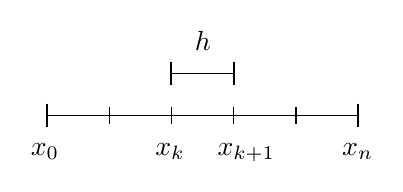
\begin{tikzpicture}[x=0.75pt,y=0.75pt,yscale=-1,xscale=1]
	%uncomment if require: \path (0,102); %set diagram left start at 0, and has height of 102

	%Straight Lines [id:da20621224248267156]
	\draw    (250,30) -- (280,30) ;
	\draw [shift={(280,30)}, rotate = 180] [color={rgb, 255:red, 0; green, 0; blue, 0 }  ][line width=0.75]    (0,5.59) -- (0,-5.59)   ;
	\draw [shift={(250,30)}, rotate = 180] [color={rgb, 255:red, 0; green, 0; blue, 0 }  ][line width=0.75]    (0,5.59) -- (0,-5.59)   ;
	%Straight Lines [id:da9554369535839922]
	\draw    (190,50) -- (340,50) (220,46) -- (220,54)(250,46) -- (250,54)(280,46) -- (280,54)(310,46) -- (310,54) ;
	\draw [shift={(340,50)}, rotate = 180] [color={rgb, 255:red, 0; green, 0; blue, 0 }  ][line width=0.75]    (0,5.59) -- (0,-5.59)   ;
	\draw [shift={(190,50)}, rotate = 180] [color={rgb, 255:red, 0; green, 0; blue, 0 }  ][line width=0.75]    (0,5.59) -- (0,-5.59)   ;

	% Text Node
	%\draw (187,22.4) node [anchor=north west][inner sep=0.75pt]    {$x_0$};
	% Text Node
	%\draw (337,22.4) node [anchor=north west][inner sep=0.75pt]    {$x_n$};
	% Text Node
	\draw (181,62.4) node [anchor=north west][inner sep=0.75pt]    {$x_0$};
	% Text Node
	\draw (241,62.4) node [anchor=north west][inner sep=0.75pt]    {$x_{k}$};
	% Text Node
	\draw (271,62.4) node [anchor=north west][inner sep=0.75pt]    {$x_{k+1}$};
	% Text Node
	\draw (260,8) node [anchor=north west][inner sep=0.75pt]    {$h$};
	% Text Node
	\draw (331,62.4) node [anchor=north west][inner sep=0.75pt]    {$x_{n}$};


	\end{tikzpicture}
\end{figure}

I nodi sono definiti da 
\begin{equation*}
    x_{i}=x_0+ih,\quad i=0,\dots,n
\end{equation*}

È possibile dimostrare che per i nodi equispaziati $|\omega_{n+1}|\le \frac{h^{n+1}} 4 n!$. Valutiamo quindi l'errore massimo nell'intervallo $I$:
\begin{multline*}
    \|E_n\|_\infty=\|f(x)-\Pi_n f(x)\|_\infty \le \frac{\|\omega_{n+1}(x)\|_\infty}{(n+1)!}\| f^{(n+1)}(x) \|_\infty\\
    \le   \frac{1}{(n+1)!} \frac{h^{n+1}}{4}\ n!\ \| \!f^{(n+1)}(x) \|_\infty
    =\underbrace{\frac{h^{n+1}}{4(n+1)}}_A \ \underbrace{\| \!f^{(n+1)}(x) \|_\infty}_B
\end{multline*}
Il termine $A$ tende a $0$ per $n\to\infty$, ma non sappiamo nulla del termine $B$: se dovesse tendere a $\infty$ più velocemente di $A$, allora l'approssimazione polinomiale diventerebbe meno accurata quando usiamo polinomi di grado superiore.

\textit{Controesempio (Fenomeno di Runge).}
Consideriamo la cosiddetta funzione di Runge, definita come:
\begin{equation*}
f:[ -5,5]\rightarrow \mathbb{R} \quad f(x) =\frac{1}{1+x^{2}}.
\end{equation*}
Se si prova a interpolare la \textbf{funzione di Runge}\index{funzione!di Runge} su un set di nodi equispaziati, per $n$ che cresce si generano delle oscillazioni via via sempre più marcate, come si vede in figura \ref{fig-runge}.

\fg[Fenomeno di Runge con polinomi interpolanti di grado $n$ crescente.]{0.6}{fig-runge}

Le oscillazioni, all'aumentare del grado, peggiorano solo \textit{in prossimità degli estremi dell'intervallo}.


 Le possibili soluzioni al fenomeno di Runge sono:
\begin{enumerate}
\item Utilizzo di \textbf{nodi non equispaziati}, concentrati agli estremi, dove ci sono oscillazioni
\item Utilizzo di \textbf{nodi equispaziati o non equispaziati} ma con metodi diversi:
\begin{enumerate}
\item \textit{Interpolazione composita}: si divide l'intervallo di approssimazione in più parti calcolando su ciascun sottointervallo un polinomio interpolante di grado $n$ non elevato $\Pi ^{n}_{h} f$.
\item \textit{Approssimazione nel senso dei minimi quadrati}, un approccio diverso dall'interpolazione vista finora.
\end{enumerate}
\end{enumerate}
\section{Utilizzo di nodi non equispaziati}
\index{nodi!non equispaziati}\label{sec:interpolazione-non-equispaziata}
\subsection{Nodi di Chebyshev-Gauss-Lobatto (CGL)}
\index{nodi!di Chebyshev-Gauss-Lobatto}
Il seguente ragionamento sarà applicato all'intervallo $I=[ -1,1]$, ma esso può essere esteso a tutto $\mathbb{R}$. Consideriamo la semicirconferenza unitaria, fissando $n$ e dividendola in $n$ spicchi di ampiezza $\frac{\pi }{n}$.
Per esempio, se $n=6$ si ha:

\begin{figure}[htpb]
	\centering
	\tikzset{every picture/.style={line width=0.75pt}} %set default line width to 0.75pt

	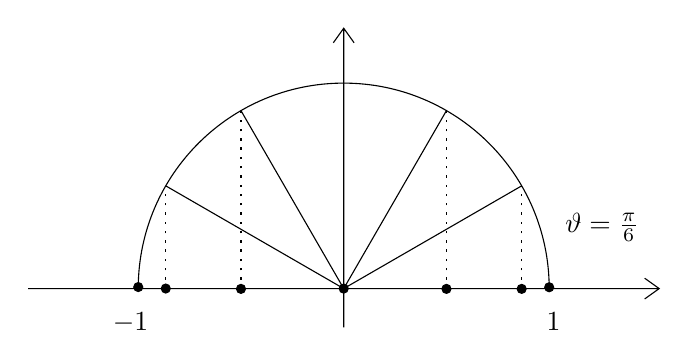
\begin{tikzpicture}[x=0.75pt,y=0.75pt,yscale=-1,xscale=1]
	%uncomment if require: \path (0,177); %set diagram left start at 0, and has height of 177

	%Shape: Axis 2D [id:dp28920976706554846]
	\draw  (147.5,134.11) -- (451.5,134.11)(299.5,8.67) -- (299.5,152.78) (444.5,129.11) -- (451.5,134.11) -- (444.5,139.11) (294.5,15.67) -- (299.5,8.67) -- (304.5,15.67)  ;
	%Shape: Circle [id:dp9498181842213234]
	\draw  [fill={rgb, 255:red, 0; green, 0; blue, 0 }  ,fill opacity=1 ] (297.33,134.11) .. controls (297.33,132.91) and (298.3,131.94) .. (299.5,131.94) .. controls (300.7,131.94) and (301.67,132.91) .. (301.67,134.11) .. controls (301.67,135.31) and (300.7,136.28) .. (299.5,136.28) .. controls (298.3,136.28) and (297.33,135.31) .. (297.33,134.11) -- cycle ;
	%Shape: Arc [id:dp9516587242954431]
	\draw  [draw opacity=0] (200.5,133.37) .. controls (200.9,79.03) and (245.07,35.11) .. (299.5,35.11) .. controls (353.96,35.11) and (398.15,79.09) .. (398.5,133.47) -- (299.5,134.11) -- cycle ; \draw   (200.5,133.37) .. controls (200.9,79.03) and (245.07,35.11) .. (299.5,35.11) .. controls (353.96,35.11) and (398.15,79.09) .. (398.5,133.47) ;
	%Shape: Boxed Line [id:dp4652733397149975]
	\draw    (299.5,134.11) -- (213.76,84.61) ;
	%Straight Lines [id:da747760306166442]
	\draw    (299.5,134.11) -- (250,48.37) ;
	%Shape: Boxed Line [id:dp3131950747001577]
	\draw    (299.5,134.11) -- (385.24,84.61) ;
	%Straight Lines [id:da26944541377482634]
	\draw    (299.5,134.11) -- (349,48.37) ;
	%Straight Lines [id:da5264596630206395]
	\draw  [dash pattern={on 0.84pt off 2.51pt}]  (349,134.25) -- (349,48.37) ;
	%Straight Lines [id:da9910633125291166]
	\draw  [dash pattern={on 0.84pt off 2.51pt}]  (385.24,134.25) -- (385.24,84.61) ;
	%Shape: Circle [id:dp28057307423967504]
	\draw  [fill={rgb, 255:red, 0; green, 0; blue, 0 }  ,fill opacity=1 ] (396.33,133.47) .. controls (396.33,132.27) and (397.3,131.3) .. (398.5,131.3) .. controls (399.69,131.3) and (400.66,132.27) .. (400.66,133.47) .. controls (400.66,134.67) and (399.69,135.64) .. (398.5,135.64) .. controls (397.3,135.64) and (396.33,134.67) .. (396.33,133.47) -- cycle ;
	%Shape: Circle [id:dp8038291186526589]
	\draw  [fill={rgb, 255:red, 0; green, 0; blue, 0 }  ,fill opacity=1 ] (198.34,133.37) .. controls (198.34,132.17) and (199.31,131.2) .. (200.5,131.2) .. controls (201.7,131.2) and (202.67,132.17) .. (202.67,133.37) .. controls (202.67,134.56) and (201.7,135.53) .. (200.5,135.53) .. controls (199.31,135.53) and (198.34,134.56) .. (198.34,133.37) -- cycle ;
	%Straight Lines [id:da9795650683884123]
	\draw  [dash pattern={on 0.84pt off 2.51pt}]  (250,134.25) -- (250,48.37) ;
	%Straight Lines [id:da5415344160854358]
	\draw  [dash pattern={on 0.84pt off 2.51pt}]  (213.76,134.25) -- (213.76,84.61) ;
	%Shape: Circle [id:dp0804362878553726]
	\draw  [fill={rgb, 255:red, 0; green, 0; blue, 0 }  ,fill opacity=1 ] (211.6,134.08) .. controls (211.6,132.89) and (212.57,131.92) .. (213.76,131.92) .. controls (214.96,131.92) and (215.93,132.89) .. (215.93,134.08) .. controls (215.93,135.28) and (214.96,136.25) .. (213.76,136.25) .. controls (212.57,136.25) and (211.6,135.28) .. (211.6,134.08) -- cycle ;
	%Shape: Circle [id:dp8087155929860674]
	\draw  [fill={rgb, 255:red, 0; green, 0; blue, 0 }  ,fill opacity=1 ] (247.83,134.25) .. controls (247.83,133.05) and (248.8,132.08) .. (250,132.08) .. controls (251.2,132.08) and (252.17,133.05) .. (252.17,134.25) .. controls (252.17,135.45) and (251.2,136.42) .. (250,136.42) .. controls (248.8,136.42) and (247.83,135.45) .. (247.83,134.25) -- cycle ;
	%Shape: Circle [id:dp21102697503346013]
	\draw  [fill={rgb, 255:red, 0; green, 0; blue, 0 }  ,fill opacity=1 ] (346.83,134.25) .. controls (346.83,133.05) and (347.8,132.08) .. (349,132.08) .. controls (350.2,132.08) and (351.17,133.05) .. (351.17,134.25) .. controls (351.17,135.45) and (350.2,136.42) .. (349,136.42) .. controls (347.8,136.42) and (346.83,135.45) .. (346.83,134.25) -- cycle ;
	%Shape: Circle [id:dp310009003820201]
	\draw  [fill={rgb, 255:red, 0; green, 0; blue, 0 }  ,fill opacity=1 ] (383.07,134.25) .. controls (383.07,133.05) and (384.04,132.08) .. (385.24,132.08) .. controls (386.43,132.08) and (387.4,133.05) .. (387.4,134.25) .. controls (387.4,135.45) and (386.43,136.42) .. (385.24,136.42) .. controls (384.04,136.42) and (383.07,135.45) .. (383.07,134.25) -- cycle ;

	% Text Node
	\draw (405,96.4) node [anchor=north west][inner sep=0.75pt]    {$\vartheta =\frac{\pi }{6}$};
	% Text Node
	\draw (187,144.4) node [anchor=north west][inner sep=0.75pt]    {$-1$};
	% Text Node
	\draw (396,144.4) node [anchor=north west][inner sep=0.75pt]    {$1$};
	\end{tikzpicture}
\end{figure}
\FloatBarrier

I nodi $x_{i}$ sono definiti come
\begin{equation}
x_{i} =-\cos\left(\frac{\pi i}{n}\right) ,\quad i=0,\dotsc ,n.
\label{eq:def-nodi-cgl}
\end{equation}
Si può dimostrare che se $f\in C^1(I)$, $\|E_{n}\|_\infty =\| \Pi _{n} f-f\|_\infty \xrightarrow{n\rightarrow \infty } 0$ con $\Pi _{n} f$ l'interpolante di Lagrange associata ai nodi di CGL.
\subsection{Nodi di Chebyshev-Gauss (CG)}
\index{nodi!di Chebyshev-Gauss}
Scegliamo solo i nodi che sono interni ad $I=[ -1,1]$, quindi tralasciando gli estremi. In questo modo:
\begin{equation}
x_{i} =-\cos\left(\frac{\pi ( 2i+1)}{2( n+1)}\right) ,\quad i=0,\dotsc ,n.
\label{eq:def-nodi-cg}
\end{equation}
Si può dimostrare che se $f$ è sufficientemente regolare, $\|E_{n}\|_\infty =\| \Pi _{n} f-f\|_\infty \xrightarrow{n\rightarrow \infty } 0$ con $\Pi _{n} f$ l'interpolante di Lagrange associata ai nodi di CG.

\textbf{NB.}
Sull'intervallo generico $[ a,b]$ i nodi di CGL e CG si ottengono da \eqref{eq:def-nodi-cgl} e da \eqref{eq:def-nodi-cg} con una trasformazione lineare:
\begin{equation*}
\hat{x}_{i} =\frac{a+b}{2} +\frac{b-a}{2} x_{i}, \quad i=0,\dotsc ,n.
\end{equation*}

\section{Interpolazione composita}
\index{interpolazione!composita}
\subsection{Interpolazione composita con nodi generici}
Assegnata $f:I\rightarrow \mathbb{R}$, vogliamo approssimare $f$ usando nodi qualunque, dividendo $[ a,b]$ in sottointervalli.
\begin{enumerate}
    \item Scegliamo i nodi di interpolazione $x_0,\dots,x_M$, dividendo quindi $I$ in $M$ sottointervalli di ampiezza $h_i$
    $$I_{i} =[ x_{i} ,x_{i+1}] \quad i=0,\dotsc ,M-1, \quad h_{i} =x_{i+1}-x_i,\quad H=\max_{i}h_i.$$
    \item Su ciascun sottointervallo $I_{i}$ approssimiamo la funzione con un polinomio $\Pi ^{H}_{k} f(x)$ di interpolazione di Lagrange di grado $k\geqslant 1$, con $k$ \textit{non troppo grande} in modo da ovviare ai problemi di oscillazione.
\end{enumerate}
Quindi il polinomio di interpolazione composita $\Pi ^{H}_{k} f(x)$ soddisfa le seguenti proprietà:
\begin{itemize}
    \item $\Pi ^{H}_{k} f\in C^0([a,b])$
    \item $\Pi ^{H}_{k} f|_{I_i}\in \mathbb P^k(I_i)\quad \forall i=0,\dots ,M-1$
    \item $\Pi ^{H}_{k} f(x_i)=y_i\quad \forall i=0,\dots ,M$
\end{itemize}

\subsection{Interpolazione composita lineare}
Per $k=1$, in ogni intervallo possiamo scrivere il polinomio di interpolazione di Lagrange come
\begin{equation*}
    \Pi ^{H}_{k} f|_{I_i}(x)=f(x_i)+\frac{f(x_{i+1})-f(x_i)}{x_{i+1}-x_i}(x-x_i)
\end{equation*}
Poiché questa è un'interpolazione lineare effettuata su $2$ nodi (che essendo solo $2$ sono "equispaziati"), supponendo $f\in C^2$ possiamo usare la disuguaglianza dell'errore presentata precedentemente:
\begin{equation*}
    \|E_n\|_{\infty,I_i}=\|f(x)- \Pi ^{H}_{k} f|_{I_i}(x)\|_\infty \le \frac{h^{k+1}}{4(k+1)}\| \!f^{(k+1)}(x) \|_{\infty,I_i} = \frac{h_i^2}{8}\ \|f''(x)\|_{\infty,I_i}
\end{equation*}
Ora valutiamo l'errore nell'intero intervallo $I$, considerando il massimo che l'errore assume tra tutti gli $I_i$:
\begin{equation*}
    \|E_n\|_{\infty,I}\le \underbrace{\frac{H^2}8}_A \underbrace{\|f''(x)\|_{\infty,I}}_B
\end{equation*}
Come nel caso trattato precedentemente, il termine $A$ tende a $0$ per $M\to\infty$, ma adesso $B$ è una costante e ciò garantisce che $\|E_M\|_\infty \xrightarrow{M\to \infty}0$.
\begin{figure}[htpb]
	\centering
    \tikzset{every picture/.style={line width=0.75pt}} %set default line width to 0.75pt        
    
    \begin{tikzpicture}[x=0.75pt,y=0.75pt,yscale=-1,xscale=1]
    %uncomment if require: \path (0,235); %set diagram left start at 0, and has height of 235
    
    %Shape: Axis 2D [id:dp18444718817100658] 
    \draw  (161.5,168.37) -- (465.5,168.37)(191.9,38.67) -- (191.9,182.78) (458.5,163.37) -- (465.5,168.37) -- (458.5,173.37) (186.9,45.67) -- (191.9,38.67) -- (196.9,45.67)  ;
    %Straight Lines [id:da062172154656692125] 
    \draw    (293.33,164.67) -- (293.33,173.33) ;
    %Shape: Circle [id:dp7214422439638635] 
    \draw  [fill={rgb, 255:red, 0; green, 0; blue, 0 }  ,fill opacity=1 ] (261.17,100.17) .. controls (261.17,98.42) and (262.58,97) .. (264.33,97) .. controls (266.08,97) and (267.5,98.42) .. (267.5,100.17) .. controls (267.5,101.92) and (266.08,103.33) .. (264.33,103.33) .. controls (262.58,103.33) and (261.17,101.92) .. (261.17,100.17) -- cycle ;
    %Shape: Circle [id:dp3795620538286856] 
    \draw  [fill={rgb, 255:red, 0; green, 0; blue, 0 }  ,fill opacity=1 ] (289.17,97.67) .. controls (289.17,95.92) and (290.58,94.51) .. (292.33,94.51) .. controls (294.08,94.51) and (295.5,95.92) .. (295.5,97.67) .. controls (295.5,99.42) and (294.08,100.84) .. (292.33,100.84) .. controls (290.58,100.84) and (289.17,99.42) .. (289.17,97.67) -- cycle ;
    %Curve Lines [id:da4712863514460399] 
    \draw    (229.6,150.8) .. controls (236.4,139.2) and (244.4,127.2) .. (254.33,111.67) .. controls (263.6,99.6) and (273.87,80.94) .. (304.33,105.67) .. controls (334.8,130.4) and (390.27,140.14) .. (414.33,89.67) .. controls (425.2,65.2) and (429.6,57.6) .. (435.6,44) ;
    %Straight Lines [id:da3752186519870171] 
    \draw    (344.33,164.67) -- (344.33,173.33) ;
    %Straight Lines [id:da4559519736586207] 
    \draw    (384.33,164.67) -- (384.33,173.33) ;
    %Straight Lines [id:da8960631674092833] 
    \draw    (264.33,164.67) -- (264.33,173.33) ;
    %Straight Lines [id:da8212422896339734] 
    \draw    (424.33,164.67) -- (424.33,173.33) ;
    %Shape: Circle [id:dp7699308608601513] 
    \draw  [fill={rgb, 255:red, 0; green, 0; blue, 0 }  ,fill opacity=1 ] (341.17,125.17) .. controls (341.17,123.42) and (342.58,122) .. (344.33,122) .. controls (346.08,122) and (347.5,123.42) .. (347.5,125.17) .. controls (347.5,126.92) and (346.08,128.33) .. (344.33,128.33) .. controls (342.58,128.33) and (341.17,126.92) .. (341.17,125.17) -- cycle ;
    %Shape: Circle [id:dp7749796192574097] 
    \draw  [fill={rgb, 255:red, 0; green, 0; blue, 0 }  ,fill opacity=1 ] (381.17,120.17) .. controls (381.17,118.42) and (382.58,117) .. (384.33,117) .. controls (386.08,117) and (387.5,118.42) .. (387.5,120.17) .. controls (387.5,121.92) and (386.08,123.33) .. (384.33,123.33) .. controls (382.58,123.33) and (381.17,121.92) .. (381.17,120.17) -- cycle ;
    %Shape: Circle [id:dp21920595374543028] 
    \draw  [fill={rgb, 255:red, 0; green, 0; blue, 0 }  ,fill opacity=1 ] (421.17,68.17) .. controls (421.17,66.42) and (422.58,65) .. (424.33,65) .. controls (426.08,65) and (427.5,66.42) .. (427.5,68.17) .. controls (427.5,69.92) and (426.08,71.33) .. (424.33,71.33) .. controls (422.58,71.33) and (421.17,69.92) .. (421.17,68.17) -- cycle ;
    %Straight Lines [id:da711773099353101] 
    \draw    (344.33,183.33) -- (384.33,183.33) ;
    \draw [shift={(384.33,183.33)}, rotate = 180] [color={rgb, 255:red, 0; green, 0; blue, 0 }  ][line width=0.75]    (0,5.59) -- (0,-5.59)   ;
    \draw [shift={(344.33,183.33)}, rotate = 180] [color={rgb, 255:red, 0; green, 0; blue, 0 }  ][line width=0.75]    (0,5.59) -- (0,-5.59)   ;
    %Straight Lines [id:da2561639103232428] 
    \draw    (384.33,120.17) -- (400.75,109.17) ;
    %Straight Lines [id:da030147884442299544] 
    \draw    (384.33,120.17) -- (344.33,125.17) ;
    %Straight Lines [id:da9060532424330414] 
    \draw    (292.33,97.67) -- (344.33,125.17) ;
    %Straight Lines [id:da9160326772746151] 
    \draw    (292.33,97.67) -- (261.17,100.17) ;
    %Straight Lines [id:da7721416652906353] 
    \draw    (401.33,164.67) -- (401.33,173.33) ;
    %Shape: Circle [id:dp5685147729949077] 
    \draw  [fill={rgb, 255:red, 0; green, 0; blue, 0 }  ,fill opacity=1 ] (397.58,109.17) .. controls (397.58,107.42) and (399,106) .. (400.75,106) .. controls (402.5,106) and (403.92,107.42) .. (403.92,109.17) .. controls (403.92,110.92) and (402.5,112.33) .. (400.75,112.33) .. controls (399,112.33) and (397.58,110.92) .. (397.58,109.17) -- cycle ;
    %Straight Lines [id:da854138099346445] 
    \draw    (400.75,109.17) -- (424.33,68.17) ;
    
    % Text Node
    \draw (170,28.4) node [anchor=north west][inner sep=0.75pt]    {$y$};
    % Text Node
    \draw (477,157.4) node [anchor=north west][inner sep=0.75pt]    {$x$};
    % Text Node
    \draw (359,188.4) node [anchor=north west][inner sep=0.75pt]    {$h_{i}$};
    
    
    \end{tikzpicture}
    
	\caption{Già nel caso di interpolazione composita con $k=1$ si può notare visivamente una maggiore \textit{precisione} nell'interpolazione, data dal fatto che stiamo lavorando su tanti intervalli di ampiezza $h_i$, pur usando un banale polinomio lineare.}
\end{figure}

\subsection{Interpolazione composita di gradi superiori al primo}
Vogliamo ora generalizzare il risultato ottenuto per l'interpolazione lineare a tratti.
Poiché un polinomio di grado superiore al primo richiede più di due nodi, all'interno di ciascun sottointervallo andiamo a scegliere ulteriori nodi, che ipotizziamo equispaziati.

In maniera analoga al caso lineare possiamo applicare in ciascun sottointervallo la stima dell'errore per nodi equispaziati, ottenendo il seguente teorema.

\begin{theorem}
Sia $f\in C^{k+1}(I)$ e sia $\Pi ^{H}_{k} f(x)$ il suo polinomio di interpolazione composita. Allora:
\begin{equation*}
\left\Vert f(x) -\Pi ^{H}_{k} f(x)\right\Vert _{\infty } \leqslant \frac{H^{k+1}}{4(k+1)} \ \left\Vert f^{( k+1)}\right\Vert _{\infty }.
\end{equation*}
\end{theorem}
\textit{Osservazione.}
Nonostante l'errore tenda a $0$ più velocemente all'aumentare di $M$, le richieste di regolarità sulla funzione sono sempre più gravose. Oltretutto la regolarità di $f$ non viene rispecchiata dal polinomio di interpolazione composita, che continua ad essere solo $C^0$. Per garantire una maggiore regolarità dell'interpolante, bisogna ricorrere a oggetti più sofisticati, come le splines.

\subsection{Splines cubiche interpolatorie}
Queste funzioni soddisfano le seguenti proprietà\footnote{
Le proprietà presentate in realtà danno origine a $4M-2$ equazioni, ma bisogna dare l'identità a $4 M$ coefficienti in quanto vanno definiti $M$ polinomi di grado $3$. Per garantire l'unicità dell'approssimazione bisognerebbe dunque aggiungere 2 condizioni.}:
\begin{itemize}
    \item $S_3(x_i)=f(x_i)\quad \forall x_i$
    \item $S_3|_{I_i}\in \mathbb P^3(I_i)\quad \forall I_ i$
    \item $S_3\in C^2(I)$
\end{itemize}

Le splines cubiche sono talmente accurate che si possono usare anche per approssimare $f'$ e $f''$.
\begin{theorem}
Sia $f$ sufficientemente regolare e sia $S_3(x)$ la sua spline cubica interpolatoria. Allora per $q=0,1,2$:
\begin{equation*}
\left\Vert f^{(q)}(x) -S_3^{(q)}(x)\right\Vert _{\infty } \leqslant C_q H^{4-q} \ \left\Vert f^{(4)}(x)\right\Vert _{\infty }
\end{equation*}
\end{theorem}


% \textit{[Lezione 11 (06-04-2020)]}
\section{Stabilità del polinomio di interpolazione}
\label{sec:stabilita-pol-interpolazione}

Sia $x_{0} ,x_{1} ,\dotsc ,x_{n}$ un insieme di $n+1$ punti distinti:

\begin{figure}[htpb]
	\centering
	\tikzset{every picture/.style={line width=0.75pt}} %set default line width to 0.75pt

	\begin{tikzpicture}[x=0.75pt,y=0.75pt,yscale=-1,xscale=1]
	%uncomment if require: \path (0,206); %set diagram left start at 0, and has height of 206

	%Shape: Axis 2D [id:dp038954507211826694]
	\draw  (169.5,167.78) -- (441.5,167.78)(169.5,36.88) -- (169.5,167.78) -- cycle (434.5,162.78) -- (441.5,167.78) -- (434.5,172.78) (164.5,43.88) -- (169.5,36.88) -- (174.5,43.88)  ;
	%Straight Lines [id:da22495486660852104]
	\draw    (230.33,163.67) -- (230.33,172.33) ;
	%Straight Lines [id:da3716248754905518]
	\draw    (280.33,163.67) -- (280.33,172.33) ;
	%Straight Lines [id:da11285799476919367]
	\draw    (390.33,163.67) -- (390.33,172.33) ;
	%Shape: Circle [id:dp13795261112398616]
	\draw  [fill={rgb, 255:red, 0; green, 0; blue, 0 }  ,fill opacity=1 ] (228.17,112.51) .. controls (228.17,111.4) and (229.06,110.51) .. (230.17,110.51) .. controls (231.27,110.51) and (232.17,111.4) .. (232.17,112.51) .. controls (232.17,113.61) and (231.27,114.51) .. (230.17,114.51) .. controls (229.06,114.51) and (228.17,113.61) .. (228.17,112.51) -- cycle ;
	%Shape: Circle [id:dp9020925580317134]
	\draw  [fill={rgb, 255:red, 0; green, 0; blue, 0 }  ,fill opacity=1 ] (278.17,107.51) .. controls (278.17,106.4) and (279.06,105.51) .. (280.17,105.51) .. controls (281.27,105.51) and (282.17,106.4) .. (282.17,107.51) .. controls (282.17,108.61) and (281.27,109.51) .. (280.17,109.51) .. controls (279.06,109.51) and (278.17,108.61) .. (278.17,107.51) -- cycle ;
	%Shape: Circle [id:dp5253082829397973]
	\draw  [fill={rgb, 255:red, 0; green, 0; blue, 0 }  ,fill opacity=1 ] (388.17,91.51) .. controls (388.17,90.4) and (389.06,89.51) .. (390.17,89.51) .. controls (391.27,89.51) and (392.17,90.4) .. (392.17,91.51) .. controls (392.17,92.61) and (391.27,93.51) .. (390.17,93.51) .. controls (389.06,93.51) and (388.17,92.61) .. (388.17,91.51) -- cycle ;
	%Curve Lines [id:da009567426004889468]
	\draw    (205.6,152.8) .. controls (212.4,141.2) and (220.4,129.2) .. (230.33,113.67) .. controls (239.6,101.6) and (249.87,82.94) .. (280.33,107.67) .. controls (310.8,132.4) and (366.27,142.14) .. (390.33,91.67) .. controls (401.2,67.2) and (405.6,59.6) .. (411.6,46) ;
	%Shape: Circle [id:dp5136163342396867]
	\draw  [fill={rgb, 255:red, 0; green, 0; blue, 0 }  ,fill opacity=1 ] (228.17,121.51) .. controls (228.17,120.4) and (229.06,119.51) .. (230.17,119.51) .. controls (231.27,119.51) and (232.17,120.4) .. (232.17,121.51) .. controls (232.17,122.61) and (231.27,123.51) .. (230.17,123.51) .. controls (229.06,123.51) and (228.17,122.61) .. (228.17,121.51) -- cycle ;
	%Shape: Circle [id:dp5738347562536119]
	\draw  [fill={rgb, 255:red, 0; green, 0; blue, 0 }  ,fill opacity=1 ] (278.17,95.51) .. controls (278.17,94.4) and (279.06,93.51) .. (280.17,93.51) .. controls (281.27,93.51) and (282.17,94.4) .. (282.17,95.51) .. controls (282.17,96.61) and (281.27,97.51) .. (280.17,97.51) .. controls (279.06,97.51) and (278.17,96.61) .. (278.17,95.51) -- cycle ;
	%Shape: Circle [id:dp3104281695353788]
	\draw  [fill={rgb, 255:red, 0; green, 0; blue, 0 }  ,fill opacity=1 ] (388.17,101.51) .. controls (388.17,100.4) and (389.06,99.51) .. (390.17,99.51) .. controls (391.27,99.51) and (392.17,100.4) .. (392.17,101.51) .. controls (392.17,102.61) and (391.27,103.51) .. (390.17,103.51) .. controls (389.06,103.51) and (388.17,102.61) .. (388.17,101.51) -- cycle ;

	% Text Node
	\draw (146,27.4) node [anchor=north west][inner sep=0.75pt]    {$y$};
	% Text Node
	\draw (453,156.4) node [anchor=north west][inner sep=0.75pt]    {$x$};
	% Text Node
	\draw (223,172.4) node [anchor=north west][inner sep=0.75pt]    {$x_{0}$};
	% Text Node
	\draw (273,172.4) node [anchor=north west][inner sep=0.75pt]    {$x_{1}$};
	% Text Node
	\draw (383,172.4) node [anchor=north west][inner sep=0.75pt]    {$x_{n}$};
	% Text Node
	\draw (373.4,70.4) node [anchor=north west][inner sep=0.75pt]    {$f$};
	% Text Node
	\draw (392.17,104.91) node [anchor=north west][inner sep=0.75pt]    {$\tilde{f}$};
	% Text Node
	\draw (323,172.4) node [anchor=north west][inner sep=0.75pt]    {$\dotsc $};
	\end{tikzpicture}
\end{figure}
\FloatBarrier

Costruiamo il polinomio di interpolazione di Lagrange di $f(x)$ dato da:
\begin{equation*}
\Pi _{n} f(x) =\sum ^{n}_{i=0} f( x_{i})\mathcal{L}_{i}(x)
\end{equation*}
dove
\begin{equation*}
\mathcal{L}_{i}(x) =\prod ^{n}_{j=0,j\neq i}\frac{( x-x_{j})}{( x_{i} -x_{j})} \quad\forall i=0,\dotsc ,n.
\end{equation*}
I valori $f( x_{i})$ possono essere affetti da errori di rappresentazione al calcolatore. Consideriamo quindi il polinomio di interpolazione ottenuto perturbando le valutazioni di $f( \cdot )$ nei nodi $x_{i}$:
\begin{equation*}
\tilde{\Pi }_{n} f(x) =\sum ^{n}_{i=0}\tilde{f}( x_{i})\mathcal{L}_{i}(x).
\end{equation*}
Come si comporta l'errore di perturbazione $\Pi _{n} f(x) -\tilde{\Pi }_{n} f(x)$ per $n\rightarrow \infty $?
\begin{align*}
\Pi _{n} f(x) -\tilde{\Pi }_{n} f(x) & =\sum ^{n}_{i=0} f( x_{i})\mathcal{L}_{i}(x) -\sum ^{n}_{i=0}\tilde{f}( x_{i})\mathcal{L}_{i}(x)\\
 & =\sum ^{n}_{i=0}\mathcal{L}_{i}(x)\underbrace{\left[ f( x_{i}) -\tilde{f}( x_{i})\right].}_{\text{errore di perturbazione}}
\end{align*}
Passando ora alla norma infinito:
\begin{align*}
\left\Vert \Pi _{n} f(x) -\tilde{\Pi }_{n} f(x)\right\Vert _{\infty } & \leqslant \underbrace{\left\Vert \sum ^{n}_{i=0}\mathcal{L}_{i}(x)\right\Vert _{\infty }}_{\Lambda _{n}(x)} \cdot \underbrace{\max_{i=1,\dotsc ,n}\left| f( x_{i}) -\tilde{f}( x_{i})\right| }_{\text{dipende solo dalla perturbazione}}\\
\left\Vert \Pi _{n} f(x) -\tilde{\Pi }_{n} f(x)\right\Vert _{\infty } & \leqslant \Lambda _{n}(x) \cdot \max_{i=1,\dotsc ,n}\left| f( x_{i}) -\tilde{f}( x_{i})\right| .
\end{align*}
Notiamo che $\Lambda_{n}(x)$ dipende solo dalla distribuzione dei nodi di approssimazione.
Essa prende il nome di \textbf{costante di Lebesgue} in quanto valore noto se i nodi sono fissati, e indipendente dalla funzione approssimata. In un certo senso è il \textit{condizionamento} del problema.

Concludiamo che l'errore di perturbazione è piccolo solo se $\Lambda_{n}(x)$ è piccola. In generale, non possiamo garantirlo, in quanto cresce per $n\rightarrow +\infty $. Si può dimostrare che
\begin{itemize}
    \item prendendo i nodi di interpolazione \textit{equispaziati}:
        \begin{equation*}
            \Lambda _{n}(x) =\left\Vert \sum ^{n}_{i=0}\mathcal{L}_{i}(x)\right\Vert _{\infty } \approx \frac{2^{n+1}}{e\, n\, (\log n+\gamma )} ,\quad\gamma \approx \frac{1}{2} ,
        \end{equation*}
    quindi con questi nodi all'aumentare di $n$ il polinomio di interpolazione diventa rapidamente più sensibile alle perturbazioni ($\approx 2^n$).
    \item Per i nodi CGL, l'andamento è logaritmico:
    $$\Lambda _{n}(x) \leqslant \frac{2}{\pi }\left[\log n+\gamma +\log\frac{8}{\pi ^{2}}\right] +\frac{\pi }{72n^{2}}.$$
    \item Per i nodi CG, analogamente vale:
    $$\Lambda _{n}(x) \leqslant \frac{2}{\pi }\left[\log( n+1) +\gamma +\log\frac{8}{\pi }\right] +\frac{\pi }{72( n+1)^{2}}.$$
        
\end{itemize}

% \textit{[Lezione 12 (07-04-2020)]}
\section{Approssimazione nel senso dei minimi quadrati}\label{sec:dati-min-quadrati}
Se i dati di cui siamo in possesso sono molto numerosi, potrebbe non aver senso cercare un'interpolazione su di essi, sia per ragioni di complessità computazionale, sia per il rischio di \textit{overfitting}, cioè la creazione di un'approssimazione eccessivamente accurata dei dati quando probabilmente essi sono affetti da errore.
In un esempio bidimensionale, potrebbe essere sufficiente una retta che descrive il comportamento qualitativo di una ``nuvola'' di punti.

Sia $( x_{i} ,y_{i})$, $i=0,\dotsc ,n$ un insieme di $n+1$ coppie di punti.


\begin{figure}[htpb]
	\centering
	\tikzset{every picture/.style={line width=0.75pt}} %set default line width to 0.75pt

	\begin{tikzpicture}[x=0.75pt,y=0.75pt,yscale=-1,xscale=1]
	%uncomment if require: \path (0,184); %set diagram left start at 0, and has height of 184

	%Shape: Axis 2D [id:dp27719212748919086]
	\draw  (146,158.49) -- (459.5,158.49)(169.5,13.88) -- (169.5,171.88) (452.5,153.49) -- (459.5,158.49) -- (452.5,163.49) (164.5,20.88) -- (169.5,13.88) -- (174.5,20.88)  ;
	%Shape: Circle [id:dp8154673289827352]
	\draw  [fill={rgb, 255:red, 0; green, 0; blue, 0 }  ,fill opacity=1 ] (215,109.75) .. controls (215,108.23) and (216.23,107) .. (217.75,107) .. controls (219.27,107) and (220.5,108.23) .. (220.5,109.75) .. controls (220.5,111.27) and (219.27,112.5) .. (217.75,112.5) .. controls (216.23,112.5) and (215,111.27) .. (215,109.75) -- cycle ;
	%Shape: Circle [id:dp2497997771583591]
	\draw  [fill={rgb, 255:red, 0; green, 0; blue, 0 }  ,fill opacity=1 ] (235,129.75) .. controls (235,128.23) and (236.23,127) .. (237.75,127) .. controls (239.27,127) and (240.5,128.23) .. (240.5,129.75) .. controls (240.5,131.27) and (239.27,132.5) .. (237.75,132.5) .. controls (236.23,132.5) and (235,131.27) .. (235,129.75) -- cycle ;
	%Shape: Circle [id:dp2629151419467781]
	\draw  [fill={rgb, 255:red, 0; green, 0; blue, 0 }  ,fill opacity=1 ] (235,89.75) .. controls (235,88.23) and (236.23,87) .. (237.75,87) .. controls (239.27,87) and (240.5,88.23) .. (240.5,89.75) .. controls (240.5,91.27) and (239.27,92.5) .. (237.75,92.5) .. controls (236.23,92.5) and (235,91.27) .. (235,89.75) -- cycle ;
	%Shape: Circle [id:dp40703778617154285]
	\draw  [fill={rgb, 255:red, 0; green, 0; blue, 0 }  ,fill opacity=1 ] (295,99.75) .. controls (295,98.23) and (296.23,97) .. (297.75,97) .. controls (299.27,97) and (300.5,98.23) .. (300.5,99.75) .. controls (300.5,101.27) and (299.27,102.5) .. (297.75,102.5) .. controls (296.23,102.5) and (295,101.27) .. (295,99.75) -- cycle ;
	%Shape: Circle [id:dp8530263048641191]
	\draw  [fill={rgb, 255:red, 0; green, 0; blue, 0 }  ,fill opacity=1 ] (265,99.75) .. controls (265,98.23) and (266.23,97) .. (267.75,97) .. controls (269.27,97) and (270.5,98.23) .. (270.5,99.75) .. controls (270.5,101.27) and (269.27,102.5) .. (267.75,102.5) .. controls (266.23,102.5) and (265,101.27) .. (265,99.75) -- cycle ;
	%Shape: Circle [id:dp3291830631551005]
	\draw  [fill={rgb, 255:red, 0; green, 0; blue, 0 }  ,fill opacity=1 ] (282,63.75) .. controls (282,62.23) and (283.23,61) .. (284.75,61) .. controls (286.27,61) and (287.5,62.23) .. (287.5,63.75) .. controls (287.5,65.27) and (286.27,66.5) .. (284.75,66.5) .. controls (283.23,66.5) and (282,65.27) .. (282,63.75) -- cycle ;
	%Shape: Circle [id:dp023574924116483986]
	\draw  [fill={rgb, 255:red, 0; green, 0; blue, 0 }  ,fill opacity=1 ] (322,73.75) .. controls (322,72.23) and (323.23,71) .. (324.75,71) .. controls (326.27,71) and (327.5,72.23) .. (327.5,73.75) .. controls (327.5,75.27) and (326.27,76.5) .. (324.75,76.5) .. controls (323.23,76.5) and (322,75.27) .. (322,73.75) -- cycle ;
	%Shape: Circle [id:dp11649449142146628]
	\draw  [fill={rgb, 255:red, 0; green, 0; blue, 0 }  ,fill opacity=1 ] (342,53.75) .. controls (342,52.23) and (343.23,51) .. (344.75,51) .. controls (346.27,51) and (347.5,52.23) .. (347.5,53.75) .. controls (347.5,55.27) and (346.27,56.5) .. (344.75,56.5) .. controls (343.23,56.5) and (342,55.27) .. (342,53.75) -- cycle ;
	%Shape: Circle [id:dp09490733528889539]
	\draw  [fill={rgb, 255:red, 0; green, 0; blue, 0 }  ,fill opacity=1 ] (332,93.75) .. controls (332,92.23) and (333.23,91) .. (334.75,91) .. controls (336.27,91) and (337.5,92.23) .. (337.5,93.75) .. controls (337.5,95.27) and (336.27,96.5) .. (334.75,96.5) .. controls (333.23,96.5) and (332,95.27) .. (332,93.75) -- cycle ;
	%Shape: Circle [id:dp2810753608488885]
	\draw  [fill={rgb, 255:red, 0; green, 0; blue, 0 }  ,fill opacity=1 ] (372,73.75) .. controls (372,72.23) and (373.23,71) .. (374.75,71) .. controls (376.27,71) and (377.5,72.23) .. (377.5,73.75) .. controls (377.5,75.27) and (376.27,76.5) .. (374.75,76.5) .. controls (373.23,76.5) and (372,75.27) .. (372,73.75) -- cycle ;
	%Shape: Circle [id:dp009238440351500232]
	\draw  [fill={rgb, 255:red, 0; green, 0; blue, 0 }  ,fill opacity=1 ] (402,33.75) .. controls (402,32.23) and (403.23,31) .. (404.75,31) .. controls (406.27,31) and (407.5,32.23) .. (407.5,33.75) .. controls (407.5,35.27) and (406.27,36.5) .. (404.75,36.5) .. controls (403.23,36.5) and (402,35.27) .. (402,33.75) -- cycle ;
	%Straight Lines [id:da3306898308124848]
	\draw  [dash pattern={on 0.84pt off 2.51pt}]  (446.5,20.88) -- (183.5,136.88) ;
	\end{tikzpicture}
\end{figure}
\FloatBarrier

Vogliamo costruire il miglior polinomio possibile $p_{m}(x)$ di grado $m< n$, che approssimi la nuvola di dati nel seguente senso:
\begin{equation}
\sum ^{n}_{i=0}( y_{i} -p_{m}( x_{i}))^{2} \leqslant \sum ^{n}_{i=0}( y_{i} -q_{m}( x_{i}))^{2} ,\quad\forall q_{m} \in \mathbb{P}^{m}.
\label{eq:condizione-min-quad}
\end{equation}
Se esiste il polinomio $p_{m}(x)$ che realizza il minimo, esso è detto polinomio di approssimazione di grado $m$ nel senso dei \textbf{minimi quadrati}.\index{minimi quadrati}

\textit{Osservazione.}
La nozione di approssimazione nel senso dei minimi quadrati è \textit{consistente} con quanto discusso fino ad ora: con $m=n$ la \eqref{eq:condizione-min-quad} diventa
\begin{equation*}
\underbrace{\sum ^{n}_{i=0}( y_{i} -\overbrace{p_{n}( x_{i})}^{\Pi _{n}( x_{i})})^{2}}_{=0} \leqslant \sum ^{n}_{i=0}( y_{i} -q_{n}( x_{i}))^{2},
\end{equation*}
ovvero otteniamo il polinomio \textit{migliore} imponendo il vincolo di passaggio su ogni singolo nodo.
Tuttavia questa scelta porta ovviamente a un polinomio di grado altissimo, e quindi fortemente instabile, come mostrato nel controesempio di Runge.
\subsection{Caso lineare}

Sia $m=1$. In tal caso si ha la \textbf{retta dei minimi quadrati}\index{retta!dei minimi quadrati} o \textbf{retta di regressione}\index{retta!di regressione}. Abbiamo $n+1$ coppie di dati $( x_{i} ,y_{i}), i=0,\dotsc ,n$. Vogliamo costruire la miglior retta possibile nell'insieme delle rette, cioè dei polinomi di primo grado. Ovvero, cerchiamo $p_{1}(x)$ tale che:
\begin{equation}
\sum ^{n}_{i=0}( y_{i} -p_{1}( x_{i}))^{2} \leqslant \sum ^{n}_{i=0}( y_{i} -q_{1}( x_{i}))^{2} ,\quad\forall q_{1} \in \mathbb{P}^{1} .
\label{eq:condizione-min-quad-1}
\end{equation}
Poiché $p_{1}(x)$ è un polinomio lineare, avrà la forma:
\begin{equation*}
p_{1}(x) =\tilde{\alpha } +\tilde{\beta } x\quad\text{con} \ \tilde{\alpha } ,\tilde{\beta } \in \mathbb{R}.
\end{equation*}
Inoltre, anche ogni altro polinomio lineare $q_{1}(x) \in \mathbb{P}^{1}$ si può scrivere come:
\begin{equation*}
q_{1}(x) =\alpha +\beta x\quad\text{con} \ \alpha ,\beta \in \mathbb{R}.
\end{equation*}
Quindi possiamo riscrivere \eqref{eq:condizione-min-quad-1}: trovare $\tilde{\alpha } ,\tilde{\beta } \in \mathbb{R}$ tali che
\begin{equation*}
\sum ^{n}_{i=0}\left( y_{i} -\left(\tilde{\alpha } +\tilde{\beta } x_{i}\right)\right)^{2} \leqslant \sum ^{n}_{i=0}( y_{i} -( \alpha +\beta x_{i}))^{2}.
\end{equation*}
Analogamente, definendo $\Phi ( \alpha ,\beta ) =\sum ^{n}_{i=0}( y_{i} -( \alpha +\beta x_{i}))^{2}$, il problema diventa trovare:
\begin{equation*}
\Phi (\tilde{\alpha } ,\tilde{\beta }) =\min_{\alpha ,\beta \in \mathbb{R}} \Phi ( \alpha ,\beta ).
\end{equation*}
Osserviamo che $\Phi ( \cdot ,\cdot )$ è un paraboloide convesso, quindi il suo unico punto di minimo si trova imponendo la condizione:
\begin{equation}
\frac{\partial \Phi ( \alpha ,\beta )}{\partial \alpha } =0 \qquad \text{e} \qquad \frac{\partial \Phi ( \alpha ,\beta )}{\partial \beta } =0.
\label{eq:condizione-min-quad-1-parab}
\end{equation}
Calcoliamo $\tilde{\alpha } ,\tilde{\beta }$ tale che \eqref{eq:condizione-min-quad-1-parab} sia soddisfatta:
\begin{equation*}
\begin{aligned}
 & \begin{cases}
\displaystyle\frac{\partial \Phi ( \alpha ,\beta )}{\partial \alpha } =\sum ^{n}_{i=0} -2( y_{i} -\alpha -\beta x_{i}) =0\\
\displaystyle\frac{\partial \Phi ( \alpha ,\beta )}{\partial \beta } =\sum ^{n}_{i=0} -2x_{i}( y_{i} -\alpha -\beta x_{i}) =0
\end{cases}\\
\Rightarrow \ \ & \begin{cases}
\displaystyle\sum ^{n}_{i=0} -2y_{i} +2\alpha +2\beta x_{i} =0\\
\displaystyle\sum ^{n}_{i=0} -2x_{i} y_{i} +2x_{i} \alpha +2\beta x^{2}_{i} =0.
\end{cases}
\end{aligned}
\end{equation*}
Abbiamo quindi ottenuto un sistema lineare di condizioni. Dividendo per $2$ e riscrivendolo in forma matriciale:
\begin{equation*}
\begin{bmatrix}
\displaystyle( n+1) & \displaystyle\sum ^{n}_{i=0} x_{i}\\
\displaystyle\sum ^{n}_{i=0} x_{i} & \displaystyle\sum ^{n}_{i=0} x^{2}_{i}
\end{bmatrix}\begin{bmatrix}
\alpha \\
\beta
\end{bmatrix} =\begin{bmatrix}
\displaystyle\sum ^{n}_{i=0} y_{i}\\
\displaystyle\sum ^{n}_{i=0} x_{i} y_{i}
\end{bmatrix}.
\end{equation*}
La soluzione $\begin{bmatrix}
\tilde{\alpha }\\
\tilde{\beta }
\end{bmatrix}$ di questo sistema lineare è il punto di minimo di $\Phi ( \alpha ,\beta )$, e fornisce quindi i coefficienti di $p_{1}(x)$. Pertanto, la retta di regressione lineare $p_{1}(x) =\tilde{\alpha } +\tilde{\beta } x$ si può calcolare attraverso la soluzione del seguente sistema lineare $( 2\times 2)$:
\begin{equation*}
\begin{bmatrix}
( n+1) & \displaystyle\sum ^{n}_{i=0} x_{i}\\
\displaystyle\sum ^{n}_{i=0} x_{i} & \displaystyle\sum ^{n}_{i=0} x^{2}_{i}
\end{bmatrix}\begin{bmatrix}
\tilde{\alpha }\\
\tilde{\beta }
\end{bmatrix} =\begin{bmatrix}
\displaystyle\sum ^{n}_{i=0} y_{i}\\
\displaystyle\sum ^{n}_{i=0} x_{i} y_{i}
\end{bmatrix}.
\end{equation*}
Osserviamo anche che la matrice è SDP, quindi il sistema ammette una e una sola soluzione come visto nei teoremi \ref{thm:esistenza-unicita-sl} e \ref{thm:A-DP-invertibile}.
\subsection{Caso generale}\label{sec:caso-gen-min-quadrati}

Sia $m\geqslant 1$. Si può procedere come prima e riscrivere $p_{m}(x)$ come:
\begin{equation*}
p_{m}(x) =\tilde{\alpha }_{0} +\tilde{\alpha }_{1} x\ +\tilde{\alpha }_{2} x^{2} +\dotsc +\tilde{\alpha }_{m} x^{m} =\sum ^{m}_{j=0}\tilde{\alpha }_{j} x^{j} \quad \text{con} \ \tilde{\alpha }_{j} \in \mathbb{R}.
\end{equation*}
Analogamente possiamo definire un apposito funzionale e minimizzarlo:
\begin{equation*}
\min_{[ \alpha _{i} ,i=0,\dotsc ,m]} \Phi ( \alpha _{0} ,\alpha _{1} ,\dotsc ,\alpha _{m}),
\end{equation*}
ossia differenziando rispetto a tutte le variabili e ponendo le derivate uguali a zero.
Si ha il sistema di $m+1$ incognite:
\begin{equation*}
\begin{cases}
\displaystyle\frac{\partial \Phi }{\partial \alpha _{0}} =0\\
\vdots \\
\displaystyle\frac{\partial \Phi }{\partial \alpha _{m}} =0
\end{cases},
\end{equation*}
allora:
\begin{equation*}
\begin{bmatrix}
( n+1) & \sum ^{n}_{i=0} x_{i} & \dotsc  & \sum ^{n}_{i=0} x^{m}_{i}\\
\sum ^{n}_{i=0} x_{i} & \sum ^{n}_{i=0} x^{2}_{i} & \dotsc  & \sum ^{n}_{i=0} x^{m+1}_{i}\\
\vdots  & \vdots  & \ddots  & \vdots \\
\sum ^{n}_{i=0} x^{m}_{i} & \sum ^{n}_{i=0} x^{m+1}_{i} & \dotsc  & \sum ^{n}_{i=0} x^{2m}_{i}
\end{bmatrix}\begin{bmatrix}
\alpha _{0}\\
\alpha _{1}\\
\vdots \\
\alpha _{m}
\end{bmatrix} =\begin{bmatrix}
\sum ^{n}_{i=0} y_{i}\\
\sum ^{n}_{i=0} x_{i} y_{i}\\
\vdots \\
\sum ^{n}_{i=0} x^{m}_{i} y_{i}
\end{bmatrix}.
\end{equation*}
Esso è un sistema di $( m+1)$ equazioni in $( m+1)$ incognite, detto sistema delle equazioni normali. La matrice è SDP, quindi il sistema ammette una e una sola soluzione:
\begin{equation*}
\begin{bmatrix}
\tilde{\alpha }_{0}\\
\tilde{\alpha }_{1}\\
\vdots \\
\tilde{\alpha }_{m}
\end{bmatrix}
\end{equation*}
che è l'insieme di coefficienti che identificano il polinomio di approssimazione nel senso dei minimi quadrati.
%!TEX root = ../main.tex

\chapter{Risoluzione di sistemi lineari indeterminati}

Prendiamo un sistema lineare della forma:
\begin{equation*}
A\x =\mathbf{b}
\end{equation*}
dove $A\in \mathbb{R}^{m\times n} ,\mathbf{b} \in \mathbb{R}^{m} ,\x \in \mathbb{R}^{n}$. Il sistema si dice \textbf{indeterminato}\index{sistema!indeterminato} se $m\ne n$. In particolare:
\begin{itemize}
\item \textbf{sovradeterminato}\index{sistema!sovradeterminato} se $m >n$,
\item \textbf{sottodeterminato}\index{sistema!sottodeterminato} se $m< n$.
\end{itemize}

\section{Sistemi lineari sovradeterminati}
Approfondiremo ora i sistemi sovradeterminati, caso di maggiore interesse.
Sia dunque $A\in \mathbb{R}^{m\times n} ,m\geqslant n$.
Consideriamo il sistema lineare
\begin{equation}
A\x =\mathbf{b} ,\qquad\mathbf{b} \in \mathbb{R}^{m},
\label{eq:sist-lin-sovradet}
\end{equation}
osserviamo che \eqref{eq:sist-lin-sovradet} ha soluzione nel senso classico del termine solo se il termine noto è un elemento del seguente spazio:
\begin{equation*}
\operatorname{range}(A) =\left\{\y \in \mathbb{R}^{m} \ \text{tale che} \ A\x =\y \ \text{per qualche} \ \x \in \mathbb{R}^{n}\right\}.
\end{equation*}
Dobbiamo quindi allargare il concetto di \textit{soluzione} per studiare un sistema sovradeterminato.
\begin{definition}
[Soluzione di un sistema lineare nel senso dei minimi quadrati]
\index{soluzione!ai minimi quadrati}
Dati $A\in \mathbb{R}^{m\times n}$, $m\geqslant n$, e $\mathbf{b} \in \mathbb{R}^{m}$, diciamo che $\x^{\star } \in \mathbb{R}^{n}$ è soluzione di \eqref{eq:sist-lin-sovradet} nel senso dei minimi quadrati se
\begin{equation*}
\Phi \left(\x^{\star }\right) =\min_{\x \in \mathbb{R}^{n}} \Phi (\x),
\end{equation*}
dove il funzionale da minimizzare è $\Phi (\mathbf{w}) =\Vert A\mathbf{w} -\mathbf{b}\Vert ^{2}_{2}$, il residuo nella norma euclidea.
\end{definition}
\textit{Osservazione.} Se $m=n$, la soluzione $\x^{\star }$ nel senso dei minimi quadrati coincide con la soluzione classica perché $\Phi \left(\x^{\star }\right) =0$.

Dobbiamo chiarire se la soluzione ai minimi quadrati esista e se sia unica.
\begin{lemma}
Se la soluzione $\x^{\star }$ nel senso dei minimi quadrati di un sistema lineare esiste, essa coincide con la soluzione $\x^{\star }$ nel senso classico del \textit{sistema di equazioni normali}:
\begin{equation*}
A^{T} A\x^{\star } =A^{T}\mathbf{b}.
\end{equation*}
\end{lemma}
\textit{Dimostrazione.}
Scriviamo il funzionale da minimizzare:
\begin{align*}
\Phi (\x) & =\Vert A\x -\mathbf{b}\Vert ^{2}_{2}\\
 & =( A\x -\mathbf{b})^{T}( A\x -\mathbf{b})\\
 & =\left(( A\x)^{T} -\mathbf{b}^{T}\right)( A\x -\mathbf{b})\\
 & =( A\x)^{T} A\x-\underbrace{\mathbf{b}^{T}A\x}_{\langle \mathbf{b} ,A\x \rangle } -\underbrace{( A\x)^{T}\mathbf{b}}_{\langle A\x ,\mathbf{b} \rangle } +\mathbf{b}^{T}\mathbf{b}\\
 & =\x^{T} A^{T} A\x -2( A\x)^{T}\mathbf{b} +\mathbf{b}^{T}\mathbf{b}\\
 & =\x^{T} A^{T} A\x -2\x^{T} A^{T}\mathbf{b} +\mathbf{b}^{T}\mathbf{b}.
\end{align*}
Calcoliamone poi il gradiente
\begin{equation*}
\nabla \Phi (\x) =2A^{T} A\x -2A^{T}\mathbf{b}
\end{equation*}
e poniamolo uguale a zero per trovare il minimo:
\begin{gather*}
\nabla \Phi \left(\x^{\star }\right) =0\\
\Updownarrow \\
A^{T} A\x^{\star } -A^{T}\mathbf{b} =0\\
\Updownarrow \\
A^{T} A\x^{\star } =A^{T}\mathbf{b}.
\qed
\end{gather*}

\begin{theorem}
Sia $A\in \mathbb{R}^{m\times n}$, $m\geqslant n$.
Se $A$ ha rango pieno, cioè $\operatorname{rank}(A) =n$, allora $A^{T} A\in \mathbb{R}^{n\times n}$ è una matrice SDP e quindi il sistema di equazioni normali
\begin{equation*}
A^{T} A\x^{\star } =A^{T}\mathbf{b}
\end{equation*}
ammette una e una sola soluzione.
\end{theorem}

\textit{Osservazione.} La definizione di soluzione fornita è coerente con l'approssimazione nel senso dei minimi quadrati per dati e funzioni vista nella sezione \ref{sec:dati-min-quadrati}. Infatti per $\tilde {\boldsymbol  \alpha} =[\tilde \alpha_0, \tilde \alpha_1, \dots,\tilde \alpha_m]$ vale che 
\[
\tilde {\boldsymbol{\alpha}}=\operatornamewithlimits{argmin}_{\boldsymbol \alpha \in\mathbb R^{m+1}}\sum_{i=0}^n\big (y_i-(\alpha_0+\alpha_1x_i+\dots+\alpha_mx_i^m)\big)^2=\operatornamewithlimits{argmin}_{\boldsymbol \alpha \in\mathbb R^{m+1}}\|A \boldsymbol \alpha -\mathbf y\|_2
\]
Dove
\[
    A=\begin{bmatrix}
        1&x_0&\cdots&x_0^m\\
        \vdots&\vdots&\ddots&\vdots\\
        1&x_n&\cdots&x_n^m
    \end{bmatrix}\in \mathbb R^{n\times m+1},\quad \mathbf y=\begin{bmatrix}
        y_0\\
        \vdots\\
        y_m
    \end{bmatrix}.
\]
$\tilde{\boldsymbol{\alpha}}$ sarà la soluzione del sistema delle equazioni normali $A^TA\boldsymbol{\alpha}=A^T\mathbf y$, che ritroviamo essere lo stesso presentato nella sezione \ref{sec:caso-gen-min-quadrati}:
\[
\underbrace{\begin{bmatrix}
        1 & \cdots & 1 \\
        x_0 & \cdots & x_n \\
        \vdots & \ddots & \vdots \\
        x_0^m & \cdots & x_n^m
    \end{bmatrix}}_{A^T}
    \underbrace{\begin{bmatrix}
        1&x_0&\cdots&x_0^m\\
        \vdots&\vdots&\ddots&\vdots\\
        1&x_n&\cdots&x_n^m
    \end{bmatrix}}_A=\begin{bmatrix}( n+1) & \sum ^{n}_{i=0} x_{i} & \dotsc  & \sum ^{n}_{i=0} x^{m}_{i}\\
\sum ^{n}_{i=0} x_{i} & \sum ^{n}_{i=0} x^{2}_{i} & \dotsc  & \sum ^{n}_{i=0} x^{m+1}_{i}\\
\vdots  & \vdots  & \ddots  & \vdots \\
\sum ^{n}_{i=0} x^{m}_{i} & \sum ^{n}_{i=0} x^{m+1}_{i} & \dotsc  & \sum ^{n}_{i=0} x^{2m}_{i}
\end{bmatrix}
\]
e
\[
A^T\mathbf y=\begin{bmatrix}
        1 & \cdots & 1 \\
        x_0 & \cdots & x_n \\
        \vdots & \ddots & \vdots \\
        x_0^m & \cdots & x_n^m
    \end{bmatrix}\begin{bmatrix}
        y_0\\
        \vdots\\
        y_m
    \end{bmatrix}=\begin{bmatrix}
\sum ^{n}_{i=0} y_{i}\\
\sum ^{n}_{i=0} x_{i} y_{i}\\
\vdots \\
\sum ^{n}_{i=0} x^{m}_{i} y_{i}
\end{bmatrix}
\]

La regressione polinomiale, quindi, non è altro che un caso particolare di soluzione di un sistema nel senso dei minimi quadrati.

\textit{Osservazioni.}
\begin{itemize}
    \item Se $A^{T} A\x^{\star } =A^{T}\mathbf{b}$ ammette una e una sola soluzione in senso classico, allora \eqref{eq:sist-lin-sovradet} ammette una e una sola soluzione nel senso dei minimi quadrati.
    \item In genere, la matrice $A^{T} A$ è molto mal condizionata, quindi nella pratica è spesso difficile risolvere il sistema di equazioni normali per calcolare $\x^{\star }$.
    \item Se una matrice $A$ invertibile viene rappresentata in un calcolatore, a causa degli errori di arrotondamento è possibile che $A^TA$ perda l'invertibilità. Ad esempio,
    \[
        A = \begin{bmatrix}
            1 & 1 \\
            2^{-27} & 0 \\
            0 & 2^{-27}
        \end{bmatrix},\quad \operatorname{float}(A^T A)=\begin{bmatrix}
            1 & 1\\
            1 & 1
        \end{bmatrix}
    \]
\end{itemize}
Dobbiamo quindi trovare un altro modo di procedere per la risoluzione.
\subsection{Fattorizzazione QR}
Proviamo a generalizzare il concetto di fattorizzazione $LU$, visto nella sezione \ref{sec:fattorizzazione-lu} e proprio delle matrici quadrate, anche a matrici rettangolari come $A$.
\begin{definition}
[Fattorizzazione $QR$]
\index{fattorizzazione!QR}
Sia $A\in \mathbb{R}^{m\times n}$, $m\geqslant n$.
Si dice che $A$ ammette una fattorizzazione $QR$ se esistono:
\begin{itemize}
\item $Q\in \mathbb{R}^{m\times m}$ ortogonale ($Q^{-1} =Q^{T}$);
\item $R\in \mathbb{R}^{m\times n}$ trapezoidale superiore (con le righe dalla $n+1$ in poi tutte nulle) 
\end{itemize}
tali che $$A=QR$$
\end{definition}
\begin{equation*}
\underbrace{\begin{bmatrix}
\cdot  & \cdot  & \cdot \\
\cdot  & \cdot  & \cdot \\
\cdot  & \cdot  & \cdot \\
\cdot  & \cdot  & \cdot \\
\cdot  & \cdot  & \cdot
\end{bmatrix}}_{A\in \mathbb{R}^{m\times n}} =\underbrace{\begin{bmatrix}
\cdot  & \cdot  & \cdot  & \cdot  & \cdot \\
\cdot  & \cdot  & \cdot  & \cdot  & \cdot \\
\cdot  & \cdot  & \cdot  & \cdot  & \cdot \\
\cdot  & \cdot  & \cdot  & \cdot  & \cdot \\
\cdot  & \cdot  & \cdot  & \cdot  & \cdot
\end{bmatrix}}_{Q\in \mathbb{R}^{m\times m}}\underbrace{\begin{bmatrix}
\cdot  & \cdot  & \cdot \\
0 & \cdot  & \cdot \\
0 & 0 & \cdot \\
0 & 0 & 0\\
0 & 0 & 0
\end{bmatrix}}_{R\in \mathbb{R}^{m\times n}}
\end{equation*}
\textbf{Proprietà (Fattorizzazione }$QR$\textbf{ ridotta).} \index{fattorizzazione!QR!ridotta} Sia $A\in \mathbb{R}^{m\times n}$, $m\geqslant n$, di rango massimo di cui esista la fattorizzazione $QR$. Allora esiste un'unica fattorizzazione di $A$ tale che:
\begin{equation*}
A=\tilde{Q} \ \tilde{R}
\end{equation*}
dove $\tilde{Q}$ e $\tilde{R}$ sono le sottomatrici ottenute da $Q$ e $R$ nel seguente modo:
\begin{itemize}
\item $\tilde{Q} =Q( 1:m,1:n) \in \mathbb{R}^{m\times n}$;
\item $\tilde{R} =R( 1:n,1:n) \in \mathbb{R}^{n\times n}$.
\end{itemize}

Inoltre le colonne di $\tilde{Q}$ sono vettori ortonormali e $\tilde{R}$ coincide con il fattore di Cholesky della matrice $A^{T} A$, ossia $A^{T} A=\tilde{R}^{T}\tilde{R}$.
\begin{equation*}
\underbrace{\begin{bmatrix}
\cdot  & \cdot  & \cdot \\
\cdot  & \cdot  & \cdot \\
\cdot  & \cdot  & \cdot \\
\cdot  & \cdot  & \cdot \\
\cdot  & \cdot  & \cdot
\end{bmatrix}}_{A\in \mathbb{R}^{m\times n}} =\underbrace{\begin{bmatrix}
\begin{array}{|c c c|}
\hline
\cdot  & \cdot  & \cdot \\
\cdot  & \cdot  & \cdot \\
\cdot  & \tilde{Q} & \cdot \\
\cdot  & \cdot  & \cdot \\
\cdot  & \cdot  & \cdot \\
\hline
\end{array} & \begin{array}{ c }
\cdot \\
\cdot \\
\cdot \\
\cdot \\
\cdot
\end{array} & \begin{array}{ c }
\cdot \\
\cdot \\
\cdot \\
\cdot \\
\cdot
\end{array}
\end{bmatrix}}_{Q\in \mathbb{R}^{m\times m}}\underbrace{\begin{bmatrix}
\begin{array}{|c c c|}
\hline
\cdot  & \cdot  & \cdot \\
0 & \tilde{R} & \cdot \\
0 & 0 & \cdot \\
\hline
\end{array}\\
\begin{array}{ c c c }
0 & 0 & 0
\end{array}\\
\begin{array}{ c c c }
0 & 0 & 0
\end{array}
\end{bmatrix}}_{R\in \mathbb{R}^{m\times n}}
\end{equation*}
Come usiamo $A=\tilde{Q} \ \tilde{R}$ per risolvere $A\x =\mathbf{b}$?
\begin{theorem}
Sia $A\in \mathbb{R}^{m\times n}$, $m\geqslant n$, di rango massimo, e sia $\mathbf{b} \in \mathbb{R}^{m}$. Allora esiste un'unica soluzione $\x^{\star } \in \mathbb{R}^{n}$ nel senso dei minimi quadrati del sistema sovradimensionato $A\x =\mathbf{b}$ ed essa è data da:
\begin{equation*}
\x^{\star } =\tilde{R}^{-1}\tilde{Q}^{T}\mathbf{b} \qquad \text{ovvero} \qquad \tilde{R}\x^{\star } =\tilde{Q}^{T}\mathbf{b}
\end{equation*}
dove $\tilde{Q}$ ed $\tilde{R}$ sono i fattori della decomposizione ridotta di $A$.
\end{theorem}
\begin{equation*}
\underbrace{\begin{bmatrix}
\begin{array}{|c c c|}
\hline
\cdot  & \cdot  & \cdot \\
\cdot  & \cdot  & \cdot \\
\cdot  & \tilde{Q} & \cdot \\
\cdot  & \cdot  & \cdot \\
\cdot  & \cdot  & \cdot \\
\hline
\end{array} & \begin{array}{ c }
\cdot \\
\cdot \\
\cdot \\
\cdot \\
\cdot
\end{array} & \begin{array}{ c }
\cdot \\
\cdot \\
\cdot \\
\cdot \\
\cdot
\end{array}
\end{bmatrix}}_{Q\in \mathbb{R}^{m\times m}}\underbrace{\begin{bmatrix}
\begin{array}{|c c c|}
\hline
\cdot  & \cdot  & \cdot \\
0 & \tilde{R} & \cdot \\
0 & 0 & \cdot \\
\hline
\end{array}\\
\begin{array}{ c c c }
0 & 0 & 0
\end{array}\\
\begin{array}{ c c c }
0 & 0 & 0
\end{array}
\end{bmatrix}}_{R\in \mathbb{R}^{m\times n}}\underbrace{\begin{bmatrix}
\begin{array}{ c }
\cdot \\
\cdot \\
\cdot
\end{array}
\end{bmatrix}}_{\x \in \mathbb{R}^{n}} =\underbrace{\begin{bmatrix}
\begin{array}{ c }
\cdot \\
\cdot \\
\cdot \\
\cdot \\
\cdot
\end{array}
\end{bmatrix}}_{\mathbf{b} \in \mathbb{R}^{n}}
\end{equation*}
\textit{Idea di dimostrazione.} Ci concentreremo sulla dimostrazione dell'esistenza, tralasciando quella dell'unicità. Supponendo che $A$ ammetta una fattorizzazione $QR$, allora:
\begin{align*}
\Vert A\x -\mathbf{b}\Vert ^{2}_{2} & =\Vert QR\x -\mathbf{b}\Vert ^{2}_{2} & \\
 & =\left\Vert Q^{T} QR\x -Q^{T}\mathbf{b}\right\Vert ^{2}_{2} & \Vert \mathbf{z}\Vert _{2} =\left\Vert Q^{T}\mathbf{z}\right\Vert _{2} \ \forall \mathbf{z}\\
 & =\left\Vert R\x -Q^{T}\mathbf{b}\right\Vert ^{2}_{2} & \text{($Q$ è ortogonale)}\\
 & =\left\Vert \tilde{R}\x -\tilde{Q}^{T}\mathbf{b}\right\Vert ^{2}_{2} +\sum ^{m}_{i=n+1}\left[\left( Q^{T}\mathbf{b}\right)_{i}\right]^{2} & \forall \x \in \mathbb{R}^{n}.
\end{align*}
Osserviamo in particolare l'ultimo passaggio: abbiamo la norma (al quadrato, ma ciò è irrilevante) di un vettore, ovvero $R\x -Q^{T}\mathbf{b}$. Dato che la norma $2$ al quadrato è per definizione (vedi \ref{def:norma-vettore}) la somma delle componenti al quadrato, possiamo liberamente separare in due somme.
Il termine $R\x$ si separa in $\tilde{R}\x$ e una somma di zeri.
Il termine $Q^{T}\mathbf{b}$ si separa in $\tilde{Q}^{T}\mathbf{b}$ e il termine in sommatoria (si noti l'indice che va da $n+1$ a $m$).
Il minimo di $\Phi (\x)$ è raggiunto per $\x^{\star }$ che annulla tutto il termine in cui compare:
\begin{equation*}
\tilde{R}\x -\tilde{Q}^{T}\mathbf{b} =0\ \ \Rightarrow \ \ \left\Vert \tilde{R}\x -\tilde{Q}^{T}\mathbf{b}\right\Vert =0
\end{equation*}
e dunque $\x^{\star }$ soddisfa
\begin{gather*}
\tilde{R}\x^{\star } -\tilde{Q}^{T}\mathbf{b} =0\ \ \Rightarrow \ \ \x^{\star } =\tilde{R}^{-1}\tilde{Q}^{T}\mathbf{b}.
\qed
\end{gather*}
\textit{Osservazione.} Il costo di calcolare la fattorizzazione $QR$ è $\approx mn^{2}$. L'algoritmo per il calcolo di $Q$ è basato sull'algoritmo di Gram-Schmidt, la tecnica dall'algebra lineare per la costruzione di una base ortonormale.

\subsection{Sistemi sovradeterminati a rango non massimo}
Consideriamo ora un sistema sovradeterminato $A\x =\mathbf b$, dove $A\in \mathbb{R}^{m\times n},\ m>n$, ma $\operatorname{Rank(A)<n}$. La soluzione nel senso dei minimi quadrati non è più unica in quanto se $x^\star$ è tale da minimizzare $\Phi(x)$, anche $x^\star+z,\ \forall z\in \operatorname{Ker}(A)$ soddisfano la medesima condizione.

Occorre quindi porre un vincolo ulteriore per trovare una nozione che sia unica.

La soluzione che cerchiamo è, tra le soluzioni nel senso dei minimi quadrati, quella a norma minima.

Per trovare questa soluzione, faremo uso della \textbf{decomposizione ai valori singolari}\index{decomposizione!ai valori singolari} \footnote{in inglese \textit{SVD}, \textit{singular value decomposition}} che è una generalizzazione della decomposizione agli autovalori.

Ricordiamo che per una matrice $A\in \mathbb R^{n\times n}$ sufficientemente regolare si definisce la sua decomposizione agli autovalori, o decomposizione spettrale, data da
\begin{gather*}
    A=RDR^{-1},\quad  \text{dove} \quad D=\operatorname{diag}(\lambda_1,\dots,\lambda_n)\\R=[\x_1,\dots,\x_n], \quad \x_i=\text{autovettori di }A.
\end{gather*}

Cominciamo allora dalla definizione dei valori singolari.

\begin{definition}
    [Valori singolari]\index{valori singolari}
    Sia $A\in\mathbb R^{m\times n},\ m>n$. I suoi valori singolari sono le radici degli autovalori di $A^TA$, ovvero
    \[
    \sigma_i=\sqrt{\lambda _i(A^TA)},\quad i=1,\dots,n
    \]
\end{definition}

\begin{theorem}
    [Decomposizione ai valori singolari]
    Sia $A\in\mathbb R^{m\times n},\ m>n$. Allora $\exists U,V$ tali che 
    \[
    A = U\Sigma V^T,
    \]
    dove $U\in \mathbb R^{m\times m}$, $V\in \mathbb R^{n\times n}$, $\Sigma=\operatorname{diag}(\sigma_1,\dots,\sigma_n)$
\end{theorem}

\begin{equation*}
\underbrace{\begin{bmatrix}
\cdot  & \cdot  & \cdot \\
\cdot  & \cdot  & \cdot \\
\cdot  & \cdot  & \cdot \\
\cdot  & \cdot  & \cdot \\
\cdot  & \cdot  & \cdot
\end{bmatrix}}_{A\in \mathbb{R}^{m\times n}} =\underbrace{\begin{bmatrix}
\cdot  & \cdot  & \cdot  & \cdot  & \cdot \\
\cdot  & \cdot  & \cdot  & \cdot  & \cdot \\
\cdot  & \cdot  & \cdot  & \cdot  & \cdot \\
\cdot  & \cdot  & \cdot  & \cdot  & \cdot \\
\cdot  & \cdot  & \cdot  & \cdot  & \cdot
\end{bmatrix}}_{U\in \mathbb{R}^{m\times m}}\underbrace{\begin{bmatrix}
\sigma_1  & 0  & 0 \\
0 & \ddots  & 0 \\
0 & 0 & \sigma_n \\
0 & 0 & 0\\
0 & 0 & 0
\end{bmatrix}}_{\Sigma\in \mathbb{R}^{m\times n}}
\underbrace{\begin{bmatrix}
    \cdot  & \cdot  & \cdot \\
    \cdot  & \cdot  & \cdot \\
    \cdot  & \cdot  & \cdot \\
\end{bmatrix}}_{V^T\in\mathbb R^{n\times n}}
\end{equation*}
\textit{Osservazione.} Il costo di calcolare la decomposizione \textit{SVD} è $\approx 12 n^3$.

\begin{definition}
    [Matrice pseudoinversa]
    Siano $A,U,V$ definiti come nel teorema. Definiamo la matrice pseudoinversa di $A$
    \[
    A^\dagger =V\Sigma^\dagger U^T,\quad \text{dove} \ \Sigma^\dagger =\operatorname{diag}\left(\frac1{\sigma_1},\dots,\frac1{\sigma_n}\right)^T
    \]
\end{definition}

\begin{theorem}
    Sia $A\in \mathbb{R}^{m\times n},\ m>n$, $\operatorname{Rank(A)<n}$. La soluzione $\x^\star$ nel senso dei minimi quadrati del sistema $A\x =\mathbb b$ di norma minima soddisfa
    \[
    \x^\star =A^\dagger\mathbf  b
    \]
\end{theorem}

\section{Sistemi lineari sottodeterminati}

Trattiamo brevemente anche i sistemi sottodeterminati. Sia $A\in \mathbb R^{m\times n}$, $m<n$. Consideriamo il sistema lineare
\[
A\x =\mathbf b,\quad \mathbf b\in \mathbb R^m.
\]
Per il teorema di Rouché-Capelli la soluzione del sistema non è unica. Procediamo quindi cercando la soluzione che soddisfi una condizione aggiuntiva, cioè che abbia norma minima.
\begin{theorem}
    Siano dati $A\in \mathbb R^{n\times m},\ m<n,\ \operatorname{Rank}(A)=m,\ \mathbf b\in \mathbb R^m$. $\x^\star = A^T(AA^T)^{-1}\mathbf b$ soddisfa le seguenti proprietà:
    \begin{gather*}
        A\x^\star =\mathbf b\tag{1}\label{eq:sottodet-soluz}\\
        \x^\star = \operatornamewithlimits{argmin}_{\x \in\mathbb R^n:A\x=\mathbf b} \|\x\| \tag{2}\label{eq:sottodet-min-norma}\\
    \end{gather*}
\end{theorem}

\textit{Dimostrazione.}

Per \eqref{eq:sottodet-soluz} è sufficiente notare $A\x^\star = AA^T (AA^T)^{-1}\mathbf b=\mathbf b$.

Per \eqref{eq:sottodet-min-norma}, dimostriamo che $\|\x^\star\|^2\le \|\x\|^2\ \forall \x\in\mathbb R^n$ tale che $A\x =\mathbf b$.

Sia dunque $\x$ tale che $A\x = \mathbf b$.
\begin{multline*}
    \|\x\|^2=\|\x^\star +(\x -\x^\star)\|=(\x^\star +(\x -\x^\star))^T(\x^\star +(\x -\x^\star))=\\=\|\x^\star \|^2+\|\x-\x^\star\|^2+2\underbrace{(\x -\x^\star)^T\x^\star}_{\triangle}
\end{multline*}

Osserviamo che 
\[
\triangle=\underbrace{(\x-\x^\star)^TA^T}_{\left(A(\x-\x^\star)\right)^T}(AA^T)^{-1}\mathbf b
\]
Ma $A(\x-\x^\star)=A\x-A\x^\star =\mathbf b-\mathbf b=\mathbf 0$, quindi riprendendo l'equazione sopra
\[
\|\x\| = \|\x^\star \|^2+\underbrace{\|\x-\x^\star\|^2}_{\ge 0} + \mathbf 0\ge \|\x^\star \|^2\qed
\]

\textit{Osservazione.} La matrice $A^T(AA^T)^{-1}$ è fortemente mal condizionata, dunque è necessario procedere in modo alternativo per determinare la soluzione. Usiamo la fattorizzazione $QR$ ridotta di $A^T$. Sia dunque $A^T=\tilde Q\tilde R$. Allora riscriviamo $\x^\star$ come
\begin{multline*}
    \x^\star = A^T(AA^T)^{-1}\mathbf b = (\tilde Q \tilde R)(( \tilde Q \tilde R)^T( \tilde Q \tilde R))^{-1}\mathbf b=\\=
    (\tilde Q \tilde R)(\tilde R^T \underbrace{\tilde Q^T \tilde Q}_I \tilde R)^{-1}\mathbf b = 
    \tilde Q \underbrace{\tilde R  \tilde R^{-1}}_I(\tilde R^T)^{-1} \mathbf b = 
    \tilde Q (\tilde R^T)^{-1} \mathbf b
\end{multline*}

%!TEX root = ../main.tex
% \textit{[Lezione 13 (16-04-2020)]}
\chapter{Integrazione numerica}
Sia assegnata la funzione continua $f:[ a,b]\rightarrow \mathbb{R}$, supponiamo di volerne calcolare l'integrale definito
\begin{equation}
I(f) =\int\nolimits ^{b}_{a} f(x) \dx.
\label{eq:integrale}
\end{equation}
Calcolare analiticamente la primitiva di $f$ può essere complicato o addirittura impossibile.
L'idea è quindi quella di approssimare $f$ con un polinomio, con i metodi mostrati nel capitolo precedente, e calcolare l'integrale del polinomio approssimante:
\begin{equation*}
I(f) =\int\nolimits ^{b}_{a} f(x) \dx\approx I_{n}(f) =\int ^{b}_{a}\Pi _{n} f(x) \dx.
\end{equation*}
Se
$$\Pi _{n} f(x) =\sum\limits ^{n}_{i=0} f( x_{i})\mathcal{L}_{i}(x)$$
possiamo scrivere:
\begin{equation*}
I_{n}(f) =\underbrace{\int\limits ^{b}_{a}\sum\limits ^{n}_{i=0} f( x_{i})\mathcal{L}_{i}(x) \dx=\sum\limits ^{n}_{i=0} f( x_{i})\underbrace{\int\limits ^{b}_{a}\mathcal{L}_{i}(x) \dx.}_{\alpha _{i}}}_{\text{per linearità}}
\end{equation*}
Si noti che $\alpha _{i}$ non dipende dalla funzione che stiamo integrando, ma solo dall'intervallo di integrazione e dal $i$-esimo polinomio di Lagrange (cioè dal nodo $i$-esimo).
Quindi
\begin{equation}
I_{n}(f) =\sum\limits ^{n}_{i=0} \alpha _{i} \, f( x_{i})
\label{eq:formula-quadratura-interp}
\end{equation}
è una \textbf{formula di quadratura di tipo interpolatorio}\index{formula!di quadratura di tipo interpolatorio}.
\begin{itemize}
\item $x_{i} ,i=0,\dotsc ,n$ si chiamano \textbf{nodi di quadratura}\index{nodo!di quadratura};
\item $\alpha _{i} ,i=0,\dotsc ,n$ si chiamano \textbf{pesi di quadratura}\index{peso!di quadratura}.
\end{itemize}

Cerchiamo di quantificare l'errore compiuto approssimando l'integrale con l'interpolante: possiamo intuire che sia legato all'errore commesso nell'approssimazione del polinomio.
\section{Formule di quadratura semplici}
\subsection{Formula del punto medio}

Vediamo il caso $n=0$. Approssimiamo $f( x)$ come $\Pi _{0} f( x)$, cioè con il valore assunto nel punto medio dell'intervallo $[ a,b]$ detto $x_{0} =(a+b)/2$.
\begin{align*}
I( f) \approx I_{0}( f) & =\int\nolimits ^{b}_{a} \Pi _{0} f( x) \dx=\int\nolimits ^{b}_{a} f( x_{0})\mathcal{L}_{0}( x) \dx\\
 & =f( x_{0})\underbrace{\int\nolimits ^{b}_{a}\mathcal{L}_{0}( x) \dx}_{\alpha _{0}}\\
 & =f( x_{0}) \alpha _{0}.
\end{align*}
Il peso è quindi\footnote{Si noti che i polinomi di Lagrange saranno diversi tra i vari casi $n=0,1,2,\dotsc $ Per esempio nel caso $n=0$ è presente un solo nodo, quindi è sufficiente imporre che in $x_{0}$ valga $1$, ovvero è il polinomio costante $1$. Nel caso $n=1$ vi sono due nodi, quindi i polinomi dovranno rispettivamente valere $1$ in un nodo e $0$ nell'altro, avranno quindi espressioni diverse dal caso $n=0$.}
\begin{align*}
\alpha _{0} & =\int\nolimits ^{b}_{a}\mathcal{L}_{0}( x) \dx=\int\nolimits ^{b}_{a} \dx=[ x]^{b}_{a} =b-a,
\end{align*}
ovvero:
\begin{equation*}
I_{0}( f) =( b-a) f\left(\frac{a+b}{2}\right).
\end{equation*}

% Pattern Info

\begin{figure}[ht]
	\centering
	\tikzset{
	pattern size/.store in=\mcSize,
	pattern size = 5pt,
	pattern thickness/.store in=\mcThickness,
	pattern thickness = 0.3pt,
	pattern radius/.store in=\mcRadius,
	pattern radius = 1pt}
	\makeatletter
	\pgfutil@ifundefined{pgf@pattern@name@_ttl2ayssy}{
	\pgfdeclarepatternformonly[\mcThickness,\mcSize]{_ttl2ayssy}
	{\pgfqpoint{0pt}{-\mcThickness}}
	{\pgfpoint{\mcSize}{\mcSize}}
	{\pgfpoint{\mcSize}{\mcSize}}
	{
	\pgfsetcolor{\tikz@pattern@color}
	\pgfsetlinewidth{\mcThickness}
	\pgfpathmoveto{\pgfqpoint{0pt}{\mcSize}}
	\pgfpathlineto{\pgfpoint{\mcSize+\mcThickness}{-\mcThickness}}
	\pgfusepath{stroke}
	}}
	\makeatother
	\tikzset{every picture/.style={line width=0.75pt}} %set default line width to 0.75pt

	\begin{tikzpicture}[x=0.75pt,y=0.75pt,yscale=-1,xscale=1]
	%uncomment if require: \path (0,184); %set diagram left start at 0, and has height of 184

	%Shape: Axis 2D [id:dp6271010983380898]
	\draw  (163,138.38) -- (447.5,138.38)(182.5,28) -- (182.5,150.38) (440.5,133.38) -- (447.5,138.38) -- (440.5,143.38) (177.5,35) -- (182.5,28) -- (187.5,35)  ;
	%Shape: Rectangle [id:dp5635695594675718]
	\draw  [pattern=_ttl2ayssy,pattern size=6pt,pattern thickness=0.75pt,pattern radius=0pt, pattern color={rgb, 255:red, 155; green, 155; blue, 155}] (227.5,82.38) -- (359.5,82.38) -- (359.5,138.38) -- (227.5,138.38) -- cycle ;
	%Curve Lines [id:da6511035270825436]
	\draw [line width=1.5]    (227.5,92.38) .. controls (267.5,42.38) and (296.5,121.38) .. (359.5,63.38) ;

	% Text Node
	\draw (222,143.4) node [anchor=north west][inner sep=0.75pt]    {$a$};
	% Text Node
	\draw (354,143.4) node [anchor=north west][inner sep=0.75pt]    {$b$};
	% Text Node
	\draw (288,143.4) node [anchor=north west][inner sep=0.75pt]    {$x_{0}$};


	\end{tikzpicture}
	\caption{Formula del punto medio.}
\end{figure}

\subsection{Formula del trapezio}
Vediamo il caso $n=1$. Approssimiamo $f( x)$ come $\Pi _{1} f( x)$, cioè il polinomio di grado $1$ (una retta) che congiunge i due nodi (ovvero gli estremi), si ha
\begin{align*}
I( f) \approx I_{1}( f) & =\int\nolimits ^{b}_{a} \Pi _{1} f( x) \dx=\int\nolimits ^{b}_{a}\sum\limits ^{1}_{i=0} f( x_{i})\mathcal{L}_{i}( x) \dx\\
 & =f( a)\underbrace{\int\nolimits ^{b}_{a}\mathcal{L}_{0}( x) \dx}_{\alpha _{0}} +f( b)\underbrace{\int\nolimits ^{b}_{a}\mathcal{L}_{1}( x) \dx}_{\alpha _{1}}\\
 & =f( a) \alpha _{0} +f( b) \alpha _{1}.
\end{align*}
I pesi sono quindi
\begin{align*}
\alpha _{0} & =\int\nolimits ^{b}_{a}\mathcal{L}_{0}( x) \dx=\dotsc =\frac{b-a}{2}\\
\alpha _{1} & =\int\nolimits ^{b}_{a}\mathcal{L}_{1}( x) \dx=\dotsc =\frac{b-a}{2},
\end{align*}
ovvero:
\begin{equation*}
I_{1}( f) =( b-a)\left[\frac{f( a) +f( b)}{2}\right].
\end{equation*}

% Pattern Info

\begin{figure}[ht]
	\centering
	\tikzset{
	pattern size/.store in=\mcSize,
	pattern size = 5pt,
	pattern thickness/.store in=\mcThickness,
	pattern thickness = 0.3pt,
	pattern radius/.store in=\mcRadius,
	pattern radius = 1pt}
	\makeatletter
	\pgfutil@ifundefined{pgf@pattern@name@_d8nfo6cka}{
	\pgfdeclarepatternformonly[\mcThickness,\mcSize]{_d8nfo6cka}
	{\pgfqpoint{0pt}{-\mcThickness}}
	{\pgfpoint{\mcSize}{\mcSize}}
	{\pgfpoint{\mcSize}{\mcSize}}
	{
	\pgfsetcolor{\tikz@pattern@color}
	\pgfsetlinewidth{\mcThickness}
	\pgfpathmoveto{\pgfqpoint{0pt}{\mcSize}}
	\pgfpathlineto{\pgfpoint{\mcSize+\mcThickness}{-\mcThickness}}
	\pgfusepath{stroke}
	}}
	\makeatother
	\tikzset{every picture/.style={line width=0.75pt}} %set default line width to 0.75pt

	\begin{tikzpicture}[x=0.75pt,y=0.75pt,yscale=-1,xscale=1]
	%uncomment if require: \path (0,184); %set diagram left start at 0, and has height of 184

	%Shape: Polygon [id:ds914652478870901]
	\draw  [pattern=_d8nfo6cka,pattern size=6pt,pattern thickness=0.75pt,pattern radius=0pt, pattern color={rgb, 255:red, 155; green, 155; blue, 155}] (359.5,63.38) -- (359.5,138.38) -- (227.5,138.38) -- (227.5,92.38) -- cycle ;
	%Shape: Axis 2D [id:dp47963482701691174]
	\draw  (163,138.38) -- (447.5,138.38)(182.5,28) -- (182.5,150.38) (440.5,133.38) -- (447.5,138.38) -- (440.5,143.38) (177.5,35) -- (182.5,28) -- (187.5,35)  ;
	%Curve Lines [id:da17986572961517844]
	\draw [line width=1.5]    (227.5,92.38) .. controls (267.5,42.38) and (296.5,121.38) .. (359.5,63.38) ;

	% Text Node
	\draw (222,143.4) node [anchor=north west][inner sep=0.75pt]    {$a=x_{0}$};
	% Text Node
	\draw (354,143.4) node [anchor=north west][inner sep=0.75pt]    {$b=x_{1}$};
	\end{tikzpicture}
	\caption{Formula del trapezio.}
\end{figure}

\subsection{Formula di Cavalieri-Simpson}
Vediamo infine il caso $n=2$. Approssimiamo $f( x)$ come $\Pi _{2} f( x)$, cioè il polinomio di grado $2$ (una parabola) che congiunge i tre nodi, ovvero gli estremi e il punto medio dell'intervallo $[ a,b]$:
\begin{align*}
I( f) \approx I_{2}( f) & =\int\nolimits ^{b}_{a} \Pi _{2} f( x) \dx=\int\nolimits ^{b}_{a}\sum\limits ^{2}_{i=0} f( x_{i})\mathcal{L}_{i}( x) \dx\\
 & =f( a)\underbrace{\int\nolimits ^{b}_{a}\mathcal{L}_{0}( x) \dx}_{\alpha _{0}} +f\left(\frac{a+b}{2}\right)\underbrace{\int\nolimits ^{b}_{a}\mathcal{L}_{1}( x) \dx}_{\alpha _{1}} +f( b)\underbrace{\int\nolimits ^{b}_{a}\mathcal{L}_{2}( x) \dx}_{\alpha _{2}}\\
 & =f( a) \alpha _{0} +f\left(\frac{a+b}{2}\right) \alpha _{1} +f( b) \alpha _{2}.
\end{align*}
I pesi sono quindi
\begin{equation*}
\begin{aligned}
\alpha _{0} & =\int\nolimits ^{b}_{a}\mathcal{L}_{0}( x) \dx=\int\nolimits ^{b}_{a}\frac{( x-x_{1})( x-x_{2})}{( x_{0} -x_{1})( x_{0} -x_{2})} \dx=\dotsc =\frac{b-a}{6}\\
\alpha _{1} & =\int\nolimits ^{b}_{a}\mathcal{L}_{1}( x) \dx=\int\nolimits ^{b}_{a}\frac{( x-x_{2})( x-x_{0})}{( x_{1} -x_{0})( x_{1} -x_{2})} \dx=\dotsc =\frac{4}{6}( b-a)\\
\alpha _{2} & =\int\nolimits ^{b}_{a}\mathcal{L}_{2}( x) \dx=\int\nolimits ^{b}_{a}\frac{( x-x_{1})( x-x_{0})}{( x_{2} -x_{1})( x_{2} -x_{0})} \dx=\dotsc =\frac{b-a}{6},
\end{aligned}
\end{equation*}
ovvero:
\begin{equation*}
I_{2}( f) =\frac{b-a}{6}\left[ f( a) +4f\left(\frac{a+b}{2}\right) +f( b)\right].
\end{equation*}

% Pattern Info
\begin{figure}[ht]
	\centering
	\tikzset{
	pattern size/.store in=\mcSize,
	pattern size = 5pt,
	pattern thickness/.store in=\mcThickness,
	pattern thickness = 0.3pt,
	pattern radius/.store in=\mcRadius,
	pattern radius = 1pt}
	\makeatletter
	\pgfutil@ifundefined{pgf@pattern@name@_vam7h2eu6}{
	\pgfdeclarepatternformonly[\mcThickness,\mcSize]{_vam7h2eu6}
	{\pgfqpoint{0pt}{-\mcThickness}}
	{\pgfpoint{\mcSize}{\mcSize}}
	{\pgfpoint{\mcSize}{\mcSize}}
	{
	\pgfsetcolor{\tikz@pattern@color}
	\pgfsetlinewidth{\mcThickness}
	\pgfpathmoveto{\pgfqpoint{0pt}{\mcSize}}
	\pgfpathlineto{\pgfpoint{\mcSize+\mcThickness}{-\mcThickness}}
	\pgfusepath{stroke}
	}}
	\makeatother
	\tikzset{every picture/.style={line width=0.75pt}} %set default line width to 0.75pt

	\begin{tikzpicture}[x=0.75pt,y=0.75pt,yscale=-1,xscale=1]
	%uncomment if require: \path (0,184); %set diagram left start at 0, and has height of 184

	%Shape: Polygon Curved [id:ds0373113295724965]
	\draw  [pattern=_vam7h2eu6,pattern size=6pt,pattern thickness=0.75pt,pattern radius=0pt, pattern color={rgb, 255:red, 155; green, 155; blue, 155}] (227.5,99.38) .. controls (236.25,74.75) and (270.25,27.5) .. (292.75,22.75) .. controls (315.25,18) and (341.75,43.75) .. (359.5,70.38) .. controls (360.25,100.25) and (359.25,117.25) .. (359.5,145.38) .. controls (317.25,145.75) and (279.25,144.75) .. (227.5,145.38) .. controls (227.25,125.75) and (227.75,113.75) .. (227.5,99.38) -- cycle ;
	%Shape: Axis 2D [id:dp6749680858828806]
	\draw  (163,145.38) -- (447.5,145.38)(182.5,35) -- (182.5,157.38) (440.5,140.38) -- (447.5,145.38) -- (440.5,150.38) (177.5,42) -- (182.5,35) -- (187.5,42)  ;
	%Curve Lines [id:da5621088598250055]
	\draw [line width=1.5]    (227.5,99.38) .. controls (272.5,68.5) and (280.25,18.25) .. (307.25,17.25) .. controls (334.25,16.25) and (350.5,43.5) .. (359.5,70.38) ;
	%Straight Lines [id:da2688120029207004]
	\draw  [dash pattern={on 0.84pt off 2.51pt}]  (293.5,145.38) -- (293.5,22.75) ;

	% Text Node
	\draw (222,150.4) node [anchor=north west][inner sep=0.75pt]    {$a=x_{0}$};
	% Text Node
	\draw (354,150.4) node [anchor=north west][inner sep=0.75pt]    {$b=x_{1}$};
	\end{tikzpicture}
	\caption{Formula di Cavalieri-Simpson.}
\end{figure}

\section{Errore delle formule di quadratura semplici}
Studiamo l'accuratezza delle approssimazioni appena enunciate.
\begin{definition}
[Errore di quadratura]
\index{errore!di quadratura}
Siano
$$
  I(f) =\int ^{b}_{a} f(x) \dx
  \quad \text{e} \quad
  I_{n}(f) =\sum\limits ^{n}_{i=0} f( x_{i}) \alpha _{i}.
$$
Definiamo l'\textbf{errore di quadratura} come
\begin{equation*}
E_{n}(f) \coloneqq I(f) -I_{n}(f).
\end{equation*}
\end{definition}
\begin{definition}
[Grado di esattezza]
\index{grado!di esattezza}
Diciamo che una formula di quadratura ha \textbf{grado di esattezza} $r\geqslant 0$ se
\begin{equation*}
E_{n}( p_{r}) =0\quad \forall p_{r} \in \mathbb{P}^{r}.
\end{equation*}
\end{definition}
Enunciamo un utile criterio per determinare il grado di esattezza di una formula di quadratura.
\begin{theorem}
Una formula di quadratura ha grado di esattezza $r$ se e solo se 
\[E_n(x^k)=0\ \forall k=0,\dots,r\]
\end{theorem}

\subsection{Calcolo dell'errore}
Ricordiamo anzitutto il teorema della media integrale pesata.
\begin{theorem}
[Media integrale pesata]
\index{media integrale pesata}
Siano $f,g\in C^{0}([ a,b])$ tali che $g$ abbia segno costante in $( a,b)$.
Allora $\exists \xi \in [ a,b]$ tale che
\begin{equation*}
\int\nolimits ^{b}_{a} f(x) g(x) \dx=f( \xi )\int\nolimits ^{b}_{a} g(x) \dx.
\end{equation*}
\end{theorem}
Riportiamo ora i teoremi relativi agli errori delle tre formule presentate, dimostrando solo il primo\footnote{Le altre due dimostrazioni sono lasciate al lettore come esercizio.}.
\begin{theorem}
[Errore della formula del punto medio]
\index{errore!della formula del punto medio}
Data $f\in C^{2}([ a,b])$, esiste $\xi \in ( a,b)$ tale che
\begin{equation*}
E_{0}(f) =\frac{1}{24} f''( \xi )( b-a)^{3}.
\end{equation*}
\end{theorem}
\textit{Dimostrazione.}
Per ipotesi abbiamo:
\begin{equation*}
I(f) =\int\nolimits ^{b}_{a} f(x) \dx \quad \text e \quad I_{0}(f) =( b-a) f\underbrace{\left(\frac{a+b}{2}\right)}_{x_{m}}.
\end{equation*}
Supponiamo che $f$ sia sufficientemente regolare in modo da calcolare l'espansione di Taylor: $\exists \eta (x) \in ( x,x_{m})$ tale che
\begin{equation*}
f(x) =f( x_{m}) +( x-x_{m}) f'( x_{m}) +\frac{( x-x_{m})^{2}}{2} f''( \eta (x)).
\end{equation*}
Calcoliamo l'errore:
\begin{align*}
E_{0}(f) &= I(f) -\ I_{0}(f) \\
  &=\int\nolimits ^{b}_{a} f(x) \dx-( b-a) f( x_{m})\\
  &=\int\nolimits ^{b}_{a}[ f(x) -f( x_{m})] \dx\\
  &=\underbrace{\int\nolimits ^{b}_{a}( x-x_{m}) f'( x_{m}) \dx}_{A} +\underbrace{\int\nolimits ^{b}_{a}\frac{( x-x_{m})^{2}}{2} f''( \eta (x)) \dx}_{B}.
\end{align*}
\begin{itemize}
\item $A$ rappresenta l'integrale di una retta che passa per il punto medio dell'intervallo, quindi $A=f'( x_{m})\int\nolimits ^{b}_{a}( x-x_{m}) \dx=0$.
\item Per $B$ utilizziamo il teorema della media integrale pesata:
\end{itemize}
\begin{align*}
B & =\frac{1}{2}\int\nolimits ^{b}_{a}( x-x_{m})^{2} f''( \eta (x)) \dx\\
 & =\frac{1}{2} f''( \xi )\int\nolimits ^{b}_{a}( x-x_{m})^{2} \dx\\
 & =\frac{1}{6} f''( \xi )\left[( x-x_{m})^{3}\right]^{b}_{a}\\
 & =\frac{1}{24} f''( \xi )( b-a)^{3}.
\end{align*}
Allora otteniamo che:
\begin{gather*}
E_{0}(f) =A+B=\frac{1}{24} f''( \xi )( b-a)^{3}.
\qed
\end{gather*}
\begin{theorem}
[Errore della formula del trapezio]
\index{errore!della formula del trapezio}
Data $f\in C^{2}([ a,b])$, esiste $\xi _{2} \in ( a,b)$ tale che
\begin{equation*}
E_{1}(f) =-\frac{1}{12} f''( \xi _{2})( b-a)^{3}.
\end{equation*}
\end{theorem}
\begin{theorem}
[Errore della formula di Cavalieri-Simpson]
\index{errore!della formula di Cavalieri-Simpson}
Data $f\in C^{4}([ a,b])$, esiste $\xi _{3} \in ( a,b)$ tale che
\begin{equation*}
E_{2}(f) =-\frac{1}{90 \cdot 32} f^{(4)}( \xi _{3})( b-a)^{5}.
\end{equation*}
\end{theorem}
\textit{Osservazioni.}
\begin{enumerate}
\item Dall'espressione dell'errore di una formula di quadratura possiamo leggere il grado di esattezza:
\begin{enumerate}
\item nel caso $n=0$, ovvero l'errore della formula del punto medio, è presente la derivata seconda. Chiaramente in qualunque punto dell'intervallo, la derivata seconda di un polinomio di grado $1$ è sempre nulla, pertanto tutti i polinomi di grado fino a $1$ sono integrati esattamente da quella formula (cioè l'errore è nullo). Il grado di esattezza è quindi $1$.
\item nel caso $n=1$, ovvero l'errore della formula del trapezio, si ragiona analogamente e si deduce che il grado di esattezza è $1$, come nella formula del punto medio.
\item nel caso $n=2$, ovvero la formula di Cavalieri-Simpson, compare la derivata quarta. Il grado di esattezza è dunque $3$.
\end{enumerate}
\item Se $n$ è pari, il grado di esattezza è $n+1$, altrimenti è $n$.
\item Una formula di quadratura a $n+1$ nodi ha sempre grado di esattezza $\geqslant n$ perché $p_{n}(x) \equiv \Pi _{n} p_{n}(x)$, ovvero un polinomio coincide con il suo polinomio approssimante.
\item Le stime indicate hanno un'utilità limitata: includono il punto $\xi$ di cui è sconosciuta la posizione esatta. Per poterle utilizzare nella pratica, dobbiamo quindi passare alla norma infinito per limitare dall'alto l'errore:
\begin{equation*}
\begin{array}{ l }
| E_{0}(x)| \leqslant \frac{1}{24}( b-a)^{3}\underbrace{\Vert f''(x)\Vert _{\infty }}_{\leqslant C}\\
| E_{1}(x)| \leqslant \frac{1}{12}( b-a)^{3}\underbrace{\Vert f''(x)\Vert _{\infty }}_{\leqslant C}\\
| E_{2}(x)| \leqslant \frac{1}{90}\frac{1}{32}( b-a)^{5}\underbrace{\left\Vert f^{(4)}(x)\right\Vert _{\infty }}_{\leqslant C}.
\end{array}
\end{equation*}
\end{enumerate}

Torniamo al caso generale di una formula di tipo interpolatorio.
\begin{equation*}
\begin{drcases}
I(f) =\int\nolimits ^{b}_{a} f(x) \dx\\
I_{n}(f) =\int\nolimits ^{b}_{a} \Pi _{n} f(x) \dx
\end{drcases} \Rightarrow E_{n}(f) =\int\nolimits ^{b}_{a}\underbrace{[ f(x) -\Pi _{n} f(x)]}_{\text{errore del polinomio}} \dx.
\end{equation*}
\textit{Osservazione.} $E_{n}(f)$ erediterà tutti i problemi di stabilità dell'errore di interpolazione del polinomio su nodi equispaziati visti nella sezione \ref{sec:stabilita-pol-interpolazione}.
Aumentando $n$ per migliorare la qualità dell'approssimazione, ci scontriamo con il fenomeno di Runge nell'approssimazione del polinomio. Possiamo risolvere il problema usando:
\begin{itemize}
\item interpolazione composita, che darà origine alle formule di quadratura composite;
\item nodi non equispaziati, che daranno origine alle formule di quadratura su nodi non equispaziati.
\end{itemize}
\section{Formule di quadratura composite}

L'idea generale è molto semplice: dividiamo l'intervallo $[a,b]$ in $N$ sottointervalli di ampiezza $H$ ed applichiamo quanto visto a ciascun sottointervallo. Già dal primo caso sarà chiaro come l'uso di formule composite permette di raggiungere risultati migliori senza che sia necessario aumentare $n$, ottenendo formule parecchio complicate, ma semplicemente raffinando la griglia di sottointervalli (diminuendo $H$).

\subsection{Punto medio composito}
\index{metodo!del punto medio composito}
Fissiamo $N\geqslant 1$ e $H=(b-a)/N$. Ogni nodo è $x_{k} =a+kH$ con $k=0,1,\dotsc ,N$.
\begin{align*}
	I(f) =\int\nolimits ^{b}_{a} f(x) \dx & =\sum\limits ^{N-1}_{k=0}\underbrace{\int\nolimits ^{x_{k+1}}_{x_{k}} f(x) \dx}_{\text{formula del punto medio}} \\
	& \approx \sum\limits ^{N-1}_{k=0} Hf\left(\frac{x_{k} +x_{k+1}}{2}\right) =I^{c}_{0}(f).
\end{align*}

% Pattern Info
\begin{figure}[ht]
	\centering
	\tikzset{
	pattern size/.store in=\mcSize,
	pattern size = 5pt,
	pattern thickness/.store in=\mcThickness,
	pattern thickness = 0.3pt,
	pattern radius/.store in=\mcRadius,
	pattern radius = 1pt}
	\makeatletter
	\pgfutil@ifundefined{pgf@pattern@name@_eb0el2vf8}{
	\pgfdeclarepatternformonly[\mcThickness,\mcSize]{_eb0el2vf8}
	{\pgfqpoint{0pt}{-\mcThickness}}
	{\pgfpoint{\mcSize}{\mcSize}}
	{\pgfpoint{\mcSize}{\mcSize}}
	{
	\pgfsetcolor{\tikz@pattern@color}
	\pgfsetlinewidth{\mcThickness}
	\pgfpathmoveto{\pgfqpoint{0pt}{\mcSize}}
	\pgfpathlineto{\pgfpoint{\mcSize+\mcThickness}{-\mcThickness}}
	\pgfusepath{stroke}
	}}
	\makeatother

	% Pattern Info

	\tikzset{
	pattern size/.store in=\mcSize,
	pattern size = 5pt,
	pattern thickness/.store in=\mcThickness,
	pattern thickness = 0.3pt,
	pattern radius/.store in=\mcRadius,
	pattern radius = 1pt}
	\makeatletter
	\pgfutil@ifundefined{pgf@pattern@name@_b6h43mq3a}{
	\pgfdeclarepatternformonly[\mcThickness,\mcSize]{_b6h43mq3a}
	{\pgfqpoint{0pt}{-\mcThickness}}
	{\pgfpoint{\mcSize}{\mcSize}}
	{\pgfpoint{\mcSize}{\mcSize}}
	{
	\pgfsetcolor{\tikz@pattern@color}
	\pgfsetlinewidth{\mcThickness}
	\pgfpathmoveto{\pgfqpoint{0pt}{\mcSize}}
	\pgfpathlineto{\pgfpoint{\mcSize+\mcThickness}{-\mcThickness}}
	\pgfusepath{stroke}
	}}
	\makeatother

	% Pattern Info

	\tikzset{
	pattern size/.store in=\mcSize,
	pattern size = 5pt,
	pattern thickness/.store in=\mcThickness,
	pattern thickness = 0.3pt,
	pattern radius/.store in=\mcRadius,
	pattern radius = 1pt}
	\makeatletter
	\pgfutil@ifundefined{pgf@pattern@name@_wmkhgalp5}{
	\pgfdeclarepatternformonly[\mcThickness,\mcSize]{_wmkhgalp5}
	{\pgfqpoint{0pt}{-\mcThickness}}
	{\pgfpoint{\mcSize}{\mcSize}}
	{\pgfpoint{\mcSize}{\mcSize}}
	{
	\pgfsetcolor{\tikz@pattern@color}
	\pgfsetlinewidth{\mcThickness}
	\pgfpathmoveto{\pgfqpoint{0pt}{\mcSize}}
	\pgfpathlineto{\pgfpoint{\mcSize+\mcThickness}{-\mcThickness}}
	\pgfusepath{stroke}
	}}
	\makeatother

	% Pattern Info

	\tikzset{
	pattern size/.store in=\mcSize,
	pattern size = 5pt,
	pattern thickness/.store in=\mcThickness,
	pattern thickness = 0.3pt,
	pattern radius/.store in=\mcRadius,
	pattern radius = 1pt}
	\makeatletter
	\pgfutil@ifundefined{pgf@pattern@name@_os5131itn}{
	\pgfdeclarepatternformonly[\mcThickness,\mcSize]{_os5131itn}
	{\pgfqpoint{0pt}{-\mcThickness}}
	{\pgfpoint{\mcSize}{\mcSize}}
	{\pgfpoint{\mcSize}{\mcSize}}
	{
	\pgfsetcolor{\tikz@pattern@color}
	\pgfsetlinewidth{\mcThickness}
	\pgfpathmoveto{\pgfqpoint{0pt}{\mcSize}}
	\pgfpathlineto{\pgfpoint{\mcSize+\mcThickness}{-\mcThickness}}
	\pgfusepath{stroke}
	}}
	\makeatother
	\tikzset{every picture/.style={line width=0.75pt}} %set default line width to 0.75pt

	\begin{tikzpicture}[x=0.75pt,y=0.75pt,yscale=-1,xscale=1]
	%uncomment if require: \path (0,231); %set diagram left start at 0, and has height of 231

	%Shape: Axis 2D [id:dp4759406840395697]
	\draw  (109.44,185.72) -- (509.06,185.72)(136.83,30.69) -- (136.83,202.58) (502.06,180.72) -- (509.06,185.72) -- (502.06,190.72) (131.83,37.69) -- (136.83,30.69) -- (141.83,37.69)  ;
	%Shape: Rectangle [id:dp16625044527752886]
	\draw  [pattern=_eb0el2vf8,pattern size=6pt,pattern thickness=0.75pt,pattern radius=0pt, pattern color={rgb, 255:red, 155; green, 155; blue, 155}] (200.04,105.91) -- (246.5,105.91) -- (246.5,185.91) -- (200.04,185.91) -- cycle ;
	%Shape: Rectangle [id:dp15579631963983576]
	\draw  [pattern=_b6h43mq3a,pattern size=6pt,pattern thickness=0.75pt,pattern radius=0pt, pattern color={rgb, 255:red, 155; green, 155; blue, 155}] (246.5,101.91) -- (292.96,101.91) -- (292.96,185.91) -- (246.5,185.91) -- cycle ;
	%Shape: Rectangle [id:dp40434679147664454]
	\draw  [pattern=_wmkhgalp5,pattern size=6pt,pattern thickness=0.75pt,pattern radius=0pt, pattern color={rgb, 255:red, 155; green, 155; blue, 155}] (292.96,109.91) -- (339.42,109.91) -- (339.42,185.91) -- (292.96,185.91) -- cycle ;
	%Shape: Rectangle [id:dp9132938977615221]
	\draw  [pattern=_os5131itn,pattern size=6pt,pattern thickness=0.75pt,pattern radius=0pt, pattern color={rgb, 255:red, 155; green, 155; blue, 155}] (339.42,93.91) -- (385.88,93.91) -- (385.88,185.91) -- (339.42,185.91) -- cycle ;
	%Curve Lines [id:da974217190813893]
	\draw [line width=1.5]    (200.04,121.11) .. controls (256.23,50.88) and (296.96,161.84) .. (385.45,80.38) ;

	% Text Node
	\draw (157.89,196.26) node [anchor=north west][inner sep=0.75pt]    {$a=x_{0}$};
	% Text Node
	\draw (382.84,197.26) node [anchor=north west][inner sep=0.75pt]    {$b=x_{N}$};
	% Text Node
	\draw (237.89,196.26) node [anchor=north west][inner sep=0.75pt]    {$x_{1}$};
	% Text Node
	\draw (287.89,196.26) node [anchor=north west][inner sep=0.75pt]    {$x_{2}$};
	% Text Node
	\draw (260.89,189.26) node [anchor=north west][inner sep=0.75pt]    {$H$};
	\end{tikzpicture}
	\caption{Punto medio composito su $N$ intervalli di ampiezza $H$.}
\end{figure}

\begin{theorem}
Data $f\in C^{2}([ a,b])$, esiste $\xi \in ( a,b)$ tale che:
\begin{equation*}
E^{c}_{0}(f) =I(f) -I^{c}_{0}(f) =\frac{b-a}{24} H^{2} f''( \xi ).
\end{equation*}
Questo ha ordine di accuratezza 2 e grado di esattezza 1.
\end{theorem}
\begin{definition}
  \index{ordine!di accuratezza}
  L'esponente di $H$ è detto \textbf{ordine di accuratezza} della formula di quadratura. Dice quanto velocemente l'errore va a $0$ al tendere di $H$ a $0$, dove $H$ è l'ampiezza dell'intervallo.
\end{definition}

\subsection{Trapezio composito}
\index{metodo!del trapezio composito}
Fissiamo $N\geqslant 1$ e $H=(b-a)/N$. Ogni nodo è $x_{k} =a+kH$ con $k=0,1,\dotsc ,N$.
\begin{align*}
I(f) =\int\nolimits ^{b}_{a} f(x) \dx & =\sum\limits ^{N-1}_{k=0}\underbrace{\int\nolimits ^{x_{k+1}}_{x_{k}} f(x) \dx}_{\text{formula del trapezio}}\\
 & \approx \sum\limits ^{N-1}_{k=0}\frac{H}{2}[ f( x_{k}) +f( x_{k+1})] =I^{c}_{1}(f).
\end{align*}


% Pattern Info

\begin{figure}[ht]
	\centering
	\tikzset{
	pattern size/.store in=\mcSize,
	pattern size = 5pt,
	pattern thickness/.store in=\mcThickness,
	pattern thickness = 0.3pt,
	pattern radius/.store in=\mcRadius,
	pattern radius = 1pt}
	\makeatletter
	\pgfutil@ifundefined{pgf@pattern@name@_g0pxuakaj}{
	\pgfdeclarepatternformonly[\mcThickness,\mcSize]{_g0pxuakaj}
	{\pgfqpoint{0pt}{-\mcThickness}}
	{\pgfpoint{\mcSize}{\mcSize}}
	{\pgfpoint{\mcSize}{\mcSize}}
	{
	\pgfsetcolor{\tikz@pattern@color}
	\pgfsetlinewidth{\mcThickness}
	\pgfpathmoveto{\pgfqpoint{0pt}{\mcSize}}
	\pgfpathlineto{\pgfpoint{\mcSize+\mcThickness}{-\mcThickness}}
	\pgfusepath{stroke}
	}}
	\makeatother
	\tikzset{every picture/.style={line width=0.75pt}} %set default line width to 0.75pt

	\begin{tikzpicture}[x=0.75pt,y=0.75pt,yscale=-1,xscale=1]
	%uncomment if require: \path (0,240); %set diagram left start at 0, and has height of 240

	%Shape: Polygon [id:ds5086256767805182]
	\draw  [pattern=_g0pxuakaj,pattern size=6pt,pattern thickness=0.75pt,pattern radius=0pt, pattern color={rgb, 255:red, 155; green, 155; blue, 155}] (385.45,80.38) -- (385.45,185.72) -- (200.04,185.72) -- (200.04,121.11) -- (247.5,96.31) -- (292.75,108.72) -- (341.5,108.31) -- cycle ;
	%Shape: Axis 2D [id:dp9717194343072217]
	\draw  (109.44,185.72) -- (509.06,185.72)(136.83,30.69) -- (136.83,202.58) (502.06,180.72) -- (509.06,185.72) -- (502.06,190.72) (131.83,37.69) -- (136.83,30.69) -- (141.83,37.69)  ;
	%Curve Lines [id:da10369460307327572]
	\draw [line width=1.5]    (200.04,121.11) .. controls (256.23,50.88) and (296.96,161.84) .. (385.45,80.38) ;
	%Straight Lines [id:da907087688566599]
	\draw    (200.04,185.72) -- (385.45,185.72) (247.04,181.72) -- (247.04,189.72)(294.04,181.72) -- (294.04,189.72)(341.04,181.72) -- (341.04,189.72) ;

	% Text Node
	\draw (157.89,196.26) node [anchor=north west][inner sep=0.75pt]    {$a=x_{0}$};
	% Text Node
	\draw (382.84,197.26) node [anchor=north west][inner sep=0.75pt]    {$b=x_{N}$};
	% Text Node
	\draw (237.89,196.26) node [anchor=north west][inner sep=0.75pt]    {$x_{1}$};
	% Text Node
	\draw (287.89,196.26) node [anchor=north west][inner sep=0.75pt]    {$x_{2}$};
	% Text Node
	\draw (260.89,189.26) node [anchor=north west][inner sep=0.75pt]    {$H$};


	\end{tikzpicture}
	\caption{Trapezio composito su $N$ intervalli di ampiezza $H$.}
\end{figure}

\begin{theorem}
Data $f\in C^{2}([ a,b])$, esiste $\eta \in ( a,b)$ tale che:
\begin{equation*}
E^{c}_{1}(f) =I(f) -I^{c}_{1}(f) =-\frac{b-a}{12} H^{2} f''( \eta ).
\end{equation*}
Questo ha ordine di accuratezza 2 e grado di esattezza 1.
\end{theorem}

\subsection{Cavalieri-Simpson composito}
\index{metodo!di Cavalieri-Simpson composito}
Fissiamo $N\geqslant 1$ e $H=\frac{b-a}{N}$. Ogni nodo è $x_{k} =a+kH$ con $k=0,1,\dotsc ,N$.
\begin{equation*}
\begin{aligned}
I(f) =\int\nolimits ^{b}_{a} f(x) \dx & =\sum\limits ^{N-1}_{k=0}\underbrace{\int\nolimits ^{x_{k+1}}_{x_{k}} f(x) \dx}_{\text{formula di CS}}\\
 & \approx \sum\limits ^{N-1}_{k=0}\frac{H}{6}\left[ f( x_{k}) +4f\left(\frac{x_{k} +x_{k+1}}{2}\right) +f( x_{k+1})\right] =I^{c}_{2}(f).
\end{aligned}
\end{equation*}
\begin{theorem}
Data $f\in C^{4}([ a,b])$, esiste $\zeta \in ( a,b)$ tale che:
\begin{equation*}
E^{c}_{2}(f) =I(f) -I^{c}_{2}(f) =-\frac{b-a}{180}\frac{1}{16} H^{4} f^{(4)}( \zeta ).
\end{equation*}
Questo ha ordine di accuratezza 4 e grado di esattezza 3.
\end{theorem}
% \textit{[Lezione 14 (20-04-2020)]}

\textit{Esempio.} Calcoliamo l'errore commesso usando la formula del punto medio su
\begin{gather*}
I(f) =\int\nolimits ^{\pi }_{0} f(x) \dx \quad \text{con} \quad f(x) =\sin(x).
\end{gather*}
Abbiamo dunque che:
\begin{gather*}
\begin{aligned}
E_{0}(f) & =\frac{1}{24}( b-a)^{3} f''( \xi ) \quad \xi \in [ a,b]\\
 & =\frac{1}{24}( \pi -0)^{3} f''( \xi )\\
| E_{0}(f)|  & \leqslant \frac{\pi ^{3}}{24}\Vert f''(x)\Vert _{\infty }=\frac{\pi ^{3} }{24} \max_{x\in [ 0,\pi ]}| -\sin x| \leqslant \frac{\pi ^{3}}{24}.
\end{aligned}
\end{gather*}

\section{Formule di Newton-Cotes (NC)}
\index{formula!di Newton-Cotes}
Sono basate sul metodo di interpolazione di Lagrange su nodi \textit{equispaziati}, nonché una generalizzazione dei metodi visti finora.
Fissiamo $n >0$ e indichiamo i nodi di quadratura con:
\begin{equation*}
x_{k} =x_{0} +kh \quad \text{con} \quad k=0,\dotsc ,n\quad \text{dove} \quad h=\frac{b-a}{n}.
\end{equation*}
% un bel nitpick: la n è diventata N? Vogliamo uniformare la notazione? (AW)
La formula generale è data da:
\begin{equation*}
I_{n}(f) =\sum\limits ^{n}_{i=0} \alpha _{i} f( x_{i}).
\end{equation*}
Le formule del punto medio, del trapezio e la formula di Simpson sono esempi di formule di Newton-Cotes, dove, rispettivamente, $n=0$, $n=1$ e $n=2$. Nel caso generale si definiscono:
\begin{itemize}
\item \textbf{formule aperte}\index{formula!aperta}, quelle in cui $x_{0} =a+h,x_{n} =b-h,h=(b-a)/(n+2)$ con $n\geqslant 0$, per esempio le formule di punto medio;
\item \textbf{formule chiuse}\index{formula!chiusa}, quelle in cui $x_{0} =a,x_{n} =b,h=(b-a)(n)$ con $n \geqslant 1$, per esempio le formule del trapezio e di Cavalieri-Simpson.
\end{itemize}

\textbf{Proprietà.}
Le formule di Newton-Cotes hanno pesi di quadratura $\alpha _{i}$ che dipendono solo da $n$ e da $h$, ma non dall’intervallo di integrazione $[ a,b]$.

\textit{Dimostrazione.}
Per semplicità consideriamo il caso delle formule di NC chiuse. Effettuiamo il seguente cambio di variabile:
\begin{equation*}
x=\Psi (t) =x_{0} +th\quad ( = a+th)
\end{equation*}
e notiamo che:
\begin{equation*}
\Psi (0) =a\qquad \Psi (n) =b\qquad \Psi (k) =x_{k} \quad \text{con} \quad k=0,\dotsc ,n.
\end{equation*}
Si vogliono ora calcolare le frazioni dei polinomi di Lagrange:
\begin{equation*}
\frac{x-x_{k}}{x_{i} -x_{k}} =\frac{a+th-( a+kh)}{a+ih-( a+kh)} =\frac{h( t-k)}{h( i-k)} =\frac{t-k}{i-k},
\end{equation*}
ma quindi
\begin{equation*}
\mathcal{L}_{i} (x)=\prod ^{n}_{k=0,k\neq i}\frac{x-x_{k}}{x_{i} -x_{k}} =\prod ^{n}_{k=0,k\neq i}\frac{t-k}{i-k} :=\varphi _{i}(t) \qquad \text{con } 0\leqslant i\leqslant n.
\end{equation*}
Usando l'uguaglianza $\alpha _{i} =\int ^{b}_{a}\mathcal{L}_{i}(x) \dx$ otteniamo che
\begin{equation*}
\alpha _{i} =\int\nolimits ^{b}_{a}\mathcal{L}_{i}(x) \dx=\int\nolimits ^{n}_{0} \varphi _{i}(t) hdt=h\int\nolimits ^{n}_{0} \varphi _{i}(t) \dt
\end{equation*}
da cui si ottiene la formula di quadratura
\begin{equation*}
I_{n}(f) =h\sum\limits ^{n}_{i=0} w_{i} f( x_{i}) ,\quad w_{i} =\int\nolimits ^{n}_{0} \varphi _{i}(t) \dt.
\qed
\end{equation*}
\textit{Osservazione.} Si può svolgere un ragionamento analogo per le formule di NC aperte, ottenendo:
\begin{equation*}
I_{n}(f) =h\sum\limits ^{n}_{i=0} w_{i} f( x_{i}) ,\quad w_{i} =\int\nolimits ^{n+1}_{-1} \varphi _{i}(t) \dt.
\end{equation*}
Nelle seguenti tabelle sono visualizzati i pesi delle formule di quadratura di Newton-Cotes chiuse e aperte:

\begin{table}[H]
\centering
{\renewcommand{\arraystretch}{1.3}% for the vertical padding
\caption{Pesi delle formule di Newton-Cotes}
\begin{subtable}{.5\linewidth}
\centering
\caption{Chiuse}
\begin{tabular}{ccccccc}
\toprule
 $n$ & $1$ & $2$ & $3$ & $4$ & $5$ & $6$ \\
\midrule
 $w_{0}$ & $\frac{1}{2}$ & $\frac{1}{3}$ & $\frac{3}{8}$ & $\frac{14}{45}$ & $\frac{95}{288}$ & $\frac{41}{140}$ \\
$w_{1}$ & $0$ & $\frac{4}{3}$ & $\frac{9}{8}$ & $\frac{64}{45}$ & $\frac{375}{288}$ & $\frac{216}{140}$ \\
$w_{2}$ & $0$ & $0$ & $0$ & $\frac{24}{45}$ & $\frac{250}{288}$ & $\frac{27}{140}$ \\
$w_{3}$ & $0$ & $0$ & $0$ & $0$ & $0$ & $\frac{272}{140}$ \\
 \bottomrule
\end{tabular}
\end{subtable}%

\begin{subtable}{.5\linewidth}
\centering
\caption{Aperte}
\begin{tabular}{ccccccc}
\toprule
 $n$ & $0$ & $1$ & $2$ & $3$ & $4$ & $5$ \\
\midrule
 $w_{0}$ & 2 & $\frac{3}{2}$ & $\frac{8}{3}$ & $\frac{5}{24}$ & $\frac{66}{20}$ & $\frac{4277}{1440}$ \\
$w_{1}$ & $0$ & $0$ & $-\frac{4}{3}$ & $\frac{5}{24}$ & $-\frac{84}{20}$ & $-\frac{3171}{1440}$ \\
$w_{2}$ & $0$ & $0$ & $0$ & $0$ & $\frac{156}{20}$ & $\frac{3934}{1440}$ \\
 \bottomrule
\end{tabular}
\end{subtable}%

}
\end{table}

\begin{theorem}
[Errore delle formule di Newton-Cotes]
\index{errore!delle formule di Newton-Cotes}
Data una formula di Newton-Cotes con $n$ pari, aperta o chiusa, e data $f\in C^{n+2}([ a,b])$, l'errore è dato da:
\begin{equation}
E_{n}(f) =\frac{M_{n}}{( n+2) !} h^{n+3} f^{( n+2)}( \xi )
\label{eq:errore-newton-cotes}
\end{equation}
dove $\xi \in ( a,b)$ e
\begin{equation*}
M_{n} =\begin{cases}
\int^{n}_{0} t\ \pi _{n+1}(t) \dt< 0 & \text{per formule chiuse}\\
\int^{n+1}_{-1} t\ \pi _{n+1}(t) \dt >0 & \text{per formule aperte}
\end{cases}
\end{equation*}
e dove
$$\pi _{n+1}(t) =\prod\limits ^{n}_{i=0}( t-i).$$
Dalla \eqref{eq:errore-newton-cotes} si deduce che il grado di esattezza è pari a $n+1$ e che l'ordine di accuratezza è $h^{n+3}$.

Similmente, per $n$ dispari e $f\in C^{n+1}([ a,b])$, si ha
\begin{equation}
E_{n}(f) =\frac{K_{n}}{( n+1) !} h^{n+2} f^{( n+1)}( \eta ),
\label{eq:errore-newton-cotes2}
\end{equation}
con
\begin{equation*}
K_{n} =\begin{cases}
\int\nolimits ^{n}_{0} \pi _{n+1}(t) \dt< 0 & \text{per formule chiuse} \\
\int\nolimits ^{n+1}_{-1} \pi _{n+1}(t) \dt >0 & \text{per formule aperte}
\end{cases}
\end{equation*}
dunque il grado di esattezza è $n$ e l'ordine di accuratezza è $h^{n+2}$.
\end{theorem}
Si noti che i pesi delle formule di NC non hanno segno costante, e ciò può essere fonte di errore di cancellazione\footnote{L'errore di cancellazione avviene quando il calcolatore somma due numeri molto piccoli e di segno opposto, a causa del fatto che esso può rappresentare solo un numero \textit{finito} di cifre decimali. Per esempio valutando le due forme del polinomio $p( x) =( x-1)^{6} =x^{6} -6x^{5} +15x^{4} -20x^{3} +15x^{2} -6x+1$ su un intervallo molto fine si noteranno delle oscillazioni, anche se il polinomio è lo stesso.}.

Inoltre da $n=9$ in poi le costanti che entrano nella formula dell'errore tendono a diventare troppo grandi, motivo per cui cercheremo di guadagnare qualcosa in termini grado di esattezza e ordine di accuratezza con le formule composite e con l'integrazione su nodi non equispazioni (Integrazione Gaussiana) nelle sezioni \ref{sec:newton-cotes-composite} e \ref{sec:integrazione-gaussiana}.

\section{Formule di Newton-Cotes composite}
\label{sec:newton-cotes-composite}
\index{formula!di Newton-Cotes composite}
Dividiamo $[ a,b]$ in $m$ sottointervalli $T_{j} =[ y_{j} ,y_{j+1}]$, tali che $y_{i} =a+jH$, essendo $H=(b-a)/m$, per $j=0,\dotsc ,m$.

\begin{figure}[htpb]
	\centering
	\tikzset{every picture/.style={line width=0.75pt}} %set default line width to 0.75pt

	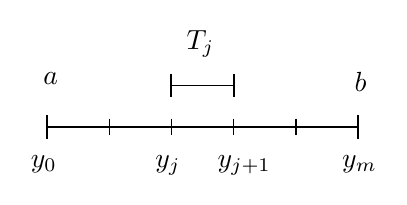
\begin{tikzpicture}[x=0.75pt,y=0.75pt,yscale=-1,xscale=1]
	%uncomment if require: \path (0,102); %set diagram left start at 0, and has height of 102

	%Straight Lines [id:da20621224248267156]
	\draw    (250,30) -- (280,30) ;
	\draw [shift={(280,30)}, rotate = 180] [color={rgb, 255:red, 0; green, 0; blue, 0 }  ][line width=0.75]    (0,5.59) -- (0,-5.59)   ;
	\draw [shift={(250,30)}, rotate = 180] [color={rgb, 255:red, 0; green, 0; blue, 0 }  ][line width=0.75]    (0,5.59) -- (0,-5.59)   ;
	%Straight Lines [id:da9554369535839922]
	\draw    (190,50) -- (340,50) (220,46) -- (220,54)(250,46) -- (250,54)(280,46) -- (280,54)(310,46) -- (310,54) ;
	\draw [shift={(340,50)}, rotate = 180] [color={rgb, 255:red, 0; green, 0; blue, 0 }  ][line width=0.75]    (0,5.59) -- (0,-5.59)   ;
	\draw [shift={(190,50)}, rotate = 180] [color={rgb, 255:red, 0; green, 0; blue, 0 }  ][line width=0.75]    (0,5.59) -- (0,-5.59)   ;

	% Text Node
	\draw (187,22.4) node [anchor=north west][inner sep=0.75pt]    {$a$};
	% Text Node
	\draw (337,22.4) node [anchor=north west][inner sep=0.75pt]    {$b$};
	% Text Node
	\draw (181,62.4) node [anchor=north west][inner sep=0.75pt]    {$y_{0}$};
	% Text Node
	\draw (241,62.4) node [anchor=north west][inner sep=0.75pt]    {$y_{j}$};
	% Text Node
	\draw (271,62.4) node [anchor=north west][inner sep=0.75pt]    {$y_{j+1}$};
	% Text Node
	\draw (256,2.4) node [anchor=north west][inner sep=0.75pt]    {$T_{j}$};
	% Text Node
	\draw (331,62.4) node [anchor=north west][inner sep=0.75pt]    {$y_{m}$};


	\end{tikzpicture}
\end{figure}
\FloatBarrier

Si utilizza quindi in ogni sottointervallo una formula interpolatoria avente per nodi i punti $\left\{x^{(j)}_{k} ,\ 0\leqslant k\leqslant n\right\}$ e per pesi i coefficienti $\left\{\alpha ^{(j)}_{k} ,\ 0\leqslant k\leqslant n\right\}$. Poiché
\begin{equation*}
I(f) =\int ^{b}_{a} f(x) \dx=\sum\limits ^{m-1}_{j=0}\int\nolimits _{T_{j}} f(x) \dx=\sum\limits ^{m-1}_{j=0}\int\nolimits ^{y_{j+} 1}_{y_{j}} f(x) \dx,
\end{equation*}
si può ottenere una formula di quadratura interpolatoria composita sostituendo $I(f)$ con
\begin{equation*}
I_{n,m}(f) =\sum\limits ^{m-1}_{j=0}\sum\limits ^{n}_{k=0} \alpha ^{(j)}_{k} f\left( x^{(j)}_{k}\right).
\end{equation*}
\begin{theorem}
[Errore delle formule di Newton-Cotes composite]
\index{errore!delle formule di Newton-Cotes composite}
Data una formula di Newton-Cotes composita, aperta o chiusa su ogni sottointervallo e con $n$ pari, se $f\in C^{n+2}([ a,b])$, si ha, per $\xi \in ( a,b)$:
\begin{equation*}
E_{n,m}(f) =\frac{b-a}{( n+2) !}\frac{M_{n}}{\gamma ^{n+3}_{n}} H^{n+2} f^{( n+2)}( \xi ).
\end{equation*}
Nel caso in cui $n$ sia dispari, se $f\in C^{n+1}([ a,b])$, si ha invece, per $\eta \in ( a,b)$:
\begin{equation*}
E_{n,m}(f) =\frac{b-a}{( n+1) !}\frac{K_{n}}{\gamma ^{n+2}_{n}} H^{n+1} f^{( n+1)}( \eta ).
\end{equation*}

Nelle due formule è stato definito
\begin{equation*}
\gamma _{n} =\begin{cases}
n+2 & \text{per formule aperte}\\
n & \text{per formule chiuse}.
\end{cases}
\end{equation*}
\end{theorem}

% \textit{[Lezione 15 (21-04-2020)]}
\section{Quadratura su nodi non equispaziati (Integrazione Gaussiana)}
\label{sec:integrazione-gaussiana}

Possiamo guadagnare gradi di esattezza e ordini di accuratezza usando nodi non equispaziati con le \textbf{formule di quadratura di Gauss-Legendre}\index{formula!di Gauss-Legendre} (GL) o di \textbf{Gauss-Legendre-Lobatto}\index{formula!di Gauss-Legendre-Lobatto} (GLL).

I nodi e i pesi sono scelti in modo da massimizzare il grado di esattezza.

In particolare:
\begin{equation*}
\{( x_{i} ,\alpha _{i})\}^{n}_{i=0} \ \ \rightarrow \ \ I_{n}(f) =\sum\limits ^{n}_{i=0} \alpha _{i} f( x_{i}) \ \begin{cases}
\text{g.d.e.} =( 2n+1) & \text{con GL}\\
\text{g.d.e.} =( 2n-1) & \text{con GLL.}
\end{cases}
\end{equation*}

\subsection{Nodi e pesi di Gauss-Legendre (GL)}
Poiché abbiamo $n+1$ nodi e $n+1$ pesi, bisogna imporre $2n+2$ condizioni per determinarli. Imponiamo che la formula di quadratura esattamente tutti i polinomi fino al grado $2n+1$, cioè:
\[
\begin{cases}
    \text{g.d.e.}=0\\
    \text{g.d.e.}=1\\
    \vdots\\
    \text{g.d.e.}=2n+1
\end{cases}
\]
Queste sono $2n+2$ equazioni, che permettono di determinare i \textbf{nodi di Gauss-Legendre}\index{nodi!di Gauss-Legendre} e i relativi pesi.

\textit{Esempio.} Determiniamo nodi e pesi di GL per $n=1$.
\[
\begin{cases}
    \text{g.d.e.}=0\\
    \text{g.d.e.}=1\\
    \text{g.d.e.}=2\\
    \text{g.d.e.}=3
\end{cases}\iff 
\begin{cases}
    \int_a^b 1=b-a=\alpha_0+\alpha_1\\
    \int_a^b x=\frac{b^2}2-\frac{a^2}2=\alpha_0 x_0+\alpha_1 x_1\\
    \int_a^b x^2=\frac{b^3}3-\frac{a^3}3=\alpha_0 x_0^2+\alpha_1 x_1^2\\
    \int_a^b x^3=\frac{b^4}4-\frac{a^4}4=\alpha_0 x_0^3+\alpha_1 x_1^3
\end{cases}
\]
È un sistema non lineare, difficile da risolvere. La sua soluzione è 
\[
x_1= a+\left(1-\frac1{\sqrt 3}\right)\left(\frac{b-a}2\right),\quad x_2= a+\left(1+\frac1{\sqrt 3}\right)\left(\frac{b-a}2\right),\quad \alpha_1=\alpha_2 =\frac{b-a}{2}
\]
\textit{Osservazione.} La formula di quadratura di GL è quindi una formula aperta.

\begin{theorem}
    [Errore della formula di Gauss-Legendre a 2 nodi]
    Data $f\in C^4([a,b])$, esiste $\xi_\text{G2}\in[a,b]$ tale che 
    \[
    E_\text{G2}(f)=\frac{1}{4320} (b-a)^5f^{(4)}(\xi_\text{G2})
    \]
\end{theorem}
Quindi con due nodi abbiamo prestazioni paragonabili a Cavalieri-Simpson!

\textit{Esempio.}
Integriamo su $( -1,1)$, con $n=1$. Abbiamo $2$ nodi, i cui pesi, si può verificare, sono $\alpha _{i} =\{1,1\}$ mentre i nodi sono $x_{i} =\left\{\pm 1/\sqrt{3}\right\}$. Consideriamo una $f( x) ,x\in [ -1,1]$.

\begin{figure}[ht]
	\centering
	\tikzset{every picture/.style={line width=0.75pt}} %set default line width to 0.75pt

	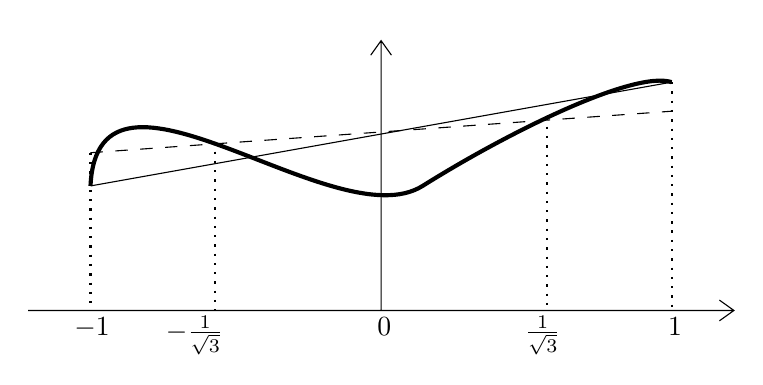
\begin{tikzpicture}[x=0.75pt,y=0.75pt,yscale=-1,xscale=1]
	%uncomment if require: \path (0,209); %set diagram left start at 0, and has height of 209

	%Shape: Axis 2D [id:dp7432814371793792]
	\draw  (130,140) -- (470,140)(300,10) -- (300,140) (463,135) -- (470,140) -- (463,145) (295,17) -- (300,10) -- (305,17)  ;
	%Straight Lines [id:da012820933470506057]
	\draw [color={rgb, 255:red, 0; green, 0; blue, 0 }  ,draw opacity=1 ][line width=0.75]  [dash pattern={on 0.84pt off 2.51pt}]  (160,64) -- (160,140) ;
	%Straight Lines [id:da052091442212324646]
	\draw [color={rgb, 255:red, 0; green, 0; blue, 0 }  ,draw opacity=1 ]   (160,80) -- (440,30) ;
	%Straight Lines [id:da9771507923640859]
	\draw [color={rgb, 255:red, 0; green, 0; blue, 0 }  ,draw opacity=1 ][line width=0.75]  [dash pattern={on 0.84pt off 2.51pt}]  (440,30) -- (440,140) ;
	%Straight Lines [id:da9708116128826352]
	\draw [color={rgb, 255:red, 0; green, 0; blue, 0 }  ,draw opacity=1 ][line width=0.75]  [dash pattern={on 0.84pt off 2.51pt}]  (380,47) -- (380,140) ;
	%Straight Lines [id:da13795556218359795]
	\draw [color={rgb, 255:red, 0; green, 0; blue, 0 }  ,draw opacity=1 ][line width=0.75]  [dash pattern={on 0.84pt off 2.51pt}]  (220,59) -- (220,140) ;
	%Straight Lines [id:da9729094667252978]
	\draw [color={rgb, 255:red, 0; green, 0; blue, 0 }  ,draw opacity=1 ] [dash pattern={on 4.5pt off 4.5pt}]  (160,64) -- (440,44) ;
	%Curve Lines [id:da34625381366262853]
	\draw [line width=1.5]    (160,80) .. controls (163.5,4.75) and (278,106.33) .. (320,80) .. controls (362,53.67) and (422,24.25) .. (440,30) ;

	% Text Node
	\draw (195,141.4) node [anchor=north west][inner sep=0.75pt]    {$-\frac{1}{\sqrt{3}}$};
	% Text Node
	\draw (368,141.4) node [anchor=north west][inner sep=0.75pt]    {$\frac{1}{\sqrt{3}}$};
	% Text Node
	\draw (437,142.4) node [anchor=north west][inner sep=0.75pt]    {$1$};
	% Text Node
	\draw (151,142.4) node [anchor=north west][inner sep=0.75pt]    {$-1$};
	% Text Node
	\draw (297,142.4) node [anchor=north west][inner sep=0.75pt]    {$0$};


	\end{tikzpicture}
	\caption{La linea spessa denota la $f( x)$, la linea sottile continua denota l'approssimazione che si ottiene con la formula del trapezio, mentre la linea sottile tratteggiata denota l'approssimazione con Gauss-Legendre.}
\end{figure}

La formula del trapezio integra in modo esatto fino a polinomi di grado $1$, mentre la \textbf{formula di Gauss-Legendre} integra in modo esatto fino a grado $3$.
\begin{align*}
I^{\text{GL}}_{1}( f) & =\sum\limits ^{2}_{i=0} \alpha _{i} f( x_{i}) =1\cdot f\left( -\frac{1}{\sqrt{3}}\right) +1\cdot f\left(\frac{1}{\sqrt{3}}\right)\\
I^{\text{trap}}_{1}( f) & =( b-a)\left[\frac{f( a) +f( b)}{2}\right] =f( -1) +f( 1)
\end{align*}

\subsection{Formule di Gauss-Legendre composite}
In modo simile a quanto fatto per le formule di Newton-Cotes, dividiamo l'intervallo $[a,b]$ in più sottointervalli, in ciascuno dei quali usiamo la formula di GL.

In questo caso, poiché GL non è una formula chiusa, in generale i polinomi interpolanti non si incontrano con continuità.

\begin{figure}[ht]
    \centering
% Pattern Info
\tikzset{
pattern size/.store in=\mcSize, 
pattern size = 5pt,
pattern thickness/.store in=\mcThickness, 
pattern thickness = 0.3pt,
pattern radius/.store in=\mcRadius, 
pattern radius = 1pt}
\makeatletter
\pgfutil@ifundefined{pgf@pattern@name@_yhmk61g9k}{
\pgfdeclarepatternformonly[\mcThickness,\mcSize]{_yhmk61g9k}
{\pgfqpoint{0pt}{-\mcThickness}}
{\pgfpoint{\mcSize}{\mcSize}}
{\pgfpoint{\mcSize}{\mcSize}}
{
\pgfsetcolor{\tikz@pattern@color}
\pgfsetlinewidth{\mcThickness}
\pgfpathmoveto{\pgfqpoint{0pt}{\mcSize}}
\pgfpathlineto{\pgfpoint{\mcSize+\mcThickness}{-\mcThickness}}
\pgfusepath{stroke}
}}
\makeatother

% Pattern Info
 
\tikzset{
pattern size/.store in=\mcSize, 
pattern size = 5pt,
pattern thickness/.store in=\mcThickness, 
pattern thickness = 0.3pt,
pattern radius/.store in=\mcRadius, 
pattern radius = 1pt}
\makeatletter
\pgfutil@ifundefined{pgf@pattern@name@_gfzj7aomp}{
\pgfdeclarepatternformonly[\mcThickness,\mcSize]{_gfzj7aomp}
{\pgfqpoint{0pt}{-\mcThickness}}
{\pgfpoint{\mcSize}{\mcSize}}
{\pgfpoint{\mcSize}{\mcSize}}
{
\pgfsetcolor{\tikz@pattern@color}
\pgfsetlinewidth{\mcThickness}
\pgfpathmoveto{\pgfqpoint{0pt}{\mcSize}}
\pgfpathlineto{\pgfpoint{\mcSize+\mcThickness}{-\mcThickness}}
\pgfusepath{stroke}
}}
\makeatother
\tikzset{every picture/.style={line width=0.75pt}} %set default line width to 0.75pt        

\begin{tikzpicture}[x=0.75pt,y=0.75pt,yscale=-1,xscale=1]
%uncomment if require: \path (0,240); %set diagram left start at 0, and has height of 240

%Shape: Polygon [id:ds6767593056546697] 
\draw  [pattern=_yhmk61g9k,pattern size=6pt,pattern thickness=0.75pt,pattern radius=0pt, pattern color={rgb, 255:red, 155; green, 155; blue, 155}] (313.67,185.6) -- (233.08,185.6) -- (231.35,70.48) -- (313.87,109.6) -- cycle ;
%Shape: Axis 2D [id:dp792326899605013] 
\draw  (109.44,185.72) -- (509.06,185.72)(136.83,30.69) -- (136.83,202.58) (502.06,180.72) -- (509.06,185.72) -- (502.06,190.72) (131.83,37.69) -- (136.83,30.69) -- (141.83,37.69)  ;
%Curve Lines [id:da6426647998245478] 
\draw [line width=1.5]    (193,117.11) .. controls (210.45,88.98) and (228.03,78.99) .. (245.08,78.67) .. controls (294.72,77.74) and (339.79,158.84) .. (363.35,112.94) .. controls (394.99,51.28) and (446.07,117.69) .. (513.82,76.38) ;
%Straight Lines [id:da06593695826492318] 
\draw  [dash pattern={on 4.5pt off 4.5pt}]  (250.27,80.67) -- (250.27,187.48) ;
%Straight Lines [id:da19011680567983746] 
\draw  [dash pattern={on 4.5pt off 4.5pt}]  (296.99,102.67) -- (296.99,185.48) ;
%Straight Lines [id:da14727304728561008] 
\draw  [dash pattern={on 4.5pt off 4.5pt}]  (333.33,123.48) -- (333.33,185.48) ;
%Straight Lines [id:da04415130495999009] 
\draw  [dash pattern={on 4.5pt off 4.5pt}]  (374.85,98.48) -- (374.85,186.48) ;
%Shape: Polygon [id:ds6999911861419973] 
\draw  [pattern=_gfzj7aomp,pattern size=6pt,pattern thickness=0.75pt,pattern radius=0pt, pattern color={rgb, 255:red, 155; green, 155; blue, 155}] (395.21,185.6) -- (313.67,185.6) -- (313.67,135.58) -- (395.72,85.48) -- cycle ;

% Text Node
\draw (212.89,195.26) node [anchor=north west][inner sep=0.75pt]    {$x_{k-1}$};
% Text Node
\draw (307.14,194.88) node [anchor=north west][inner sep=0.75pt]    {$x_{k}$};
% Text Node
\draw (397.21,197) node [anchor=north west][inner sep=0.75pt]    {$x_{k+1}$};
% Text Node
\draw (265,212.4) node [anchor=north west][inner sep=0.75pt]    {$I_{k}$};
% Text Node
\draw (342,214.4) node [anchor=north west][inner sep=0.75pt]    {$I_{k+1}$};
% Text Node
\draw (247.89,188.4) node [anchor=north west][inner sep=0.75pt]  [font=\scriptsize]  {$x_{1}^{\text G,k}$};
% Text Node
\draw (280.89,188.4) node [anchor=north west][inner sep=0.75pt]  [font=\scriptsize]  {$x_{2}^{\text G,k}$};
% Text Node
\draw (328.89,187.4) node [anchor=north west][inner sep=0.75pt]  [font=\scriptsize]  {$x_{1}^{\text G,k+1}$};
% Text Node
\draw (361.44,189) node [anchor=north west][inner sep=0.75pt]  [font=\scriptsize]  {$x_{2}^{\text G,k+1}$};
\end{tikzpicture}
\end{figure}

\begin{theorem}
    [Errore della formula di Gauss-Legendre composito a 2 nodi]
    Data $f\in C^4([a,b])$, esiste $\rho\in[a,b]$ tale che 
    \[
    E_\text{G2}^C(f)=\frac{H^4}{4320} (b-a)f^{(4)}(\rho)
    \]
\end{theorem}
Il grado di esattezza è $3$ e l'ordine di accuratezza è $4$.

\subsection{Polinomi di Legendre}
Cerchiamo un modo più semplice per trovare i nodi e pesi di GL\footnote{In realtà tali valori si trovano già tabulati in software di calcolo, per cui in genere non è necessario calcolarli.}.

Cominciamo introducendo la nozione di \textbf{polinomi ortogonali}\index{polinomio!ortogonale} rispetto a un peso, ovvero una funzione non negativa, integrabile e continua.
\begin{definition}
    Dato un insieme di polinomi $\mathcal P=\{p_k\}_{k=0}^n$, i suoi elementi sono detti \textbf{polinomi ortogonali} sull'intervallo $[a,b]$ rispetto al peso $w$ se
    \[
    \int_{a}^b p_k(x) p_m(x)w(x)\,dx=0\quad\forall k\ne x
    \]
\end{definition}

In particolare, se $w(x)\equiv 1$ e $[a,b]=[-1,1]$, i polinomi $L_k\in \mathcal P$ e tali che $L_k\in \mathbb P^k\ \forall k$ sono detti \textbf{polinomi di Legendre}\index{polinomio!di Legendre}.

Vale che
\[
\int_{-1}^{1} L_k(x) L_m(x) \, dx = \left(k + \frac{1}{2} \right)^{-1} \delta_{km},\quad \text{dove } \ \delta_{km}=\begin{cases}
    1&\text{se }k=m\\
    0&\text{se }k\ne m
\end{cases}
\]
Inoltre si può dimostrare che $\{L_k\}_{k=1}^n$ è una base per lo spazio dei polinomi di grado $n$ su $I$:
\begin{equation*}
\mathbb{P}^{n}(I) =\operatorname{span}\{L_{0}(x) ,L_{1}(x) ,\dotsc ,L_{n}(x)\} .
\end{equation*}
Presentiamo una formula ricorsiva per il calcolo dei polinomi di Legendre:
\begin{equation*}
\begin{cases}
L_{0}(x) =1\\
L_{1}(x) =x\\
L_{k+1} =\frac{2k+1}{k+1} xL_{k}(x) -\frac{k}{k+1} L_{k-1}(x) \quad \text{con} \quad k=1,2,\dots
\end{cases}
\end{equation*}

I polinomi di Legendre non sono l'unica famiglia di polinomi ortogonali: se ad esempio $w(x)=\frac{1}{\sqrt{1-x^2}}$, otteniamo i cosiddetti \textbf{polinomi di Chebyshev}\index{polinomio!di Chebyshev}.

\subsection{Approssimazione di integrali pesati}
Oltre a trovare i valori di pesi e nodi di GL, i polinomi di Legendre danno origine a una \textbf{formula di quadratura per integrali pesati}.

Approssimiamo l'integrale $I_w(f)$ in questo modo:
\[
I_w(f)=\int_{-1}^1f(x)w(x)\,dx\approx \sum_{i=0}^n f(x_i)\underbrace{\int_{-1}^1\varphi_i(x) w(x)\,dx}_{\alpha_i}=\sum _{i=0}^nf(x_i)\alpha_i,
\]
Dove gli $x_i$ sono gli zeri del polinomio di Legendre di grado $n+1$.

Il grado di esattezza della formula è $2n+1$, che si può dimostrare essere il massimo raggiungibile.

In particolare, se $w(x)\equiv 1$, troviamo i nodi di Gauss-Legendre ed i relativi pesi:
\begin{equation}
x_{i} = \text{zeri di} \ L_{n+1}(x) ,\quad \alpha _{i} =\frac{2}{( 1-x_{i})^{2}[ L_{n+1} '( x_{i})]^{2}} ,\quad i=0,\dotsc ,n.
\label{eq:nodi-gl}
\end{equation}


\subsection{Nodi e pesi di Gauss-Legendre-Lobatto (GLL)}
Come per i Gauss-Legendre, scegliamo strategicamente i nodi di quadratura, ma questa volta vogliamo che siano inclusi anche gli estremi.

Per $n\geqslant 0$, i \textbf{nodi di Gauss-Legendre-Lobatto}\index{nodi!di Gauss-Legendre-Lobatto} ed i relativi pesi sono dati da:
\begin{gather}
\begin{split}
x_{0} =-1,\quad &\left\{x_{i} \ \text{zeri di} \ L_{n} '(x) ,\quad i=1,\dotsc ,n-1\right\} ,\quad x_{n} =1,\\
&\alpha _{i} =\frac{2}{n( n+1)}\frac{1}{[ L_{n}( x_{i})]^{2}} ,\quad i=0,\dotsc ,n.
\end{split}
\label{eq:nodi-gll}
\end{gather}

Il grado di esattezza della formula è $2n-1$: due in meno di GL, poiché la scelta di due nodi (gli estremi) non è strategica.

\textbf{NB.}
Sull'intervallo generico $[ a,b]$ i nodi di GL e GLL si ottengono da \eqref{eq:nodi-gl} e da \eqref{eq:nodi-gll} con la stessa trasformazione lineare vista nella sezione \ref{sec:interpolazione-non-equispaziata} per l'interpolazione non equispaziata:
\begin{equation*}
\hat{x}_{i} =\frac{a+b}{2} +\frac{b-a}{2} x_{i}, \quad i=0,\dotsc ,n.
\end{equation*}

\subsection{Errore delle formule di GL e GLL}
\index{errore!di Gauss-Legendre}
\index{errore!di Gauss-Legendre-Lobatto}
Data $f$ sufficientemente regolare, vale la seguente rappresentazione dell'errore:
\begin{equation*}
| E_{n}(f)| \leqslant \frac{C}{n^{5}}\Vert f\Vert _{s}
\end{equation*}
dove
\begin{equation*}
\Vert f\Vert _{s} =\left(\sum\limits ^{s}_{k=0}\left\Vert f^{(k)}\right\Vert ^{2}_{L^{2}( -1,1)}\right)^{1/2}
\end{equation*}
nel quale
\begin{equation*}
\Vert f\Vert _{L^{2}( -1,1)} =\left[\int\nolimits ^{1}_{-1}[ f(x)]^{2} \dx\right]^{1/2} .
\end{equation*}

Per concludere il capitolo, presentiamo nella tabella \ref{tab:gradi-ordini} un riassunto dei principali risultati di accuratezza ed esattezza delle formule viste.

\begin{table}[ht]
\centering
{\renewcommand{\arraystretch}{1.3}% for the vertical padding
\begin{tabular}{lcc}
\toprule
   & grado di esattezza & ordine di accuratezza \\
\midrule
 Punto medio semplice & $1$ &  \\
 Trapezio semplice & $1$ &  \\
 CS semplice & $3$ &  \\
 $n$ pari & $n+1$ &  \\
 $n$ dispari & $n$ &  \\
\hline
 Punto medio composito & $1$ & $2$ \\
 Trapezio composito & $1$ & $2$ \\
 CS composito & $3$ & $4$ \\
\hline
 NC, $n$ pari & $n+1$ & $n+3$ \\
 NC, $n$ dispari & $n$ & $n+2$ \\
 NC composite, $n$ pari & $n+1$ & $n+2$ \\
 NC composite, $n$ dispari & $n$ & $n+1$ \\
\hline
 GL & $2n+1$ &  \\
 GLL & $2n-1$ &  \\
 \bottomrule
\end{tabular}
}
\caption{Tabella riassuntiva dei gradi di esattezza e ordini di accuratezza dei metodi numerici analizzati.}
\label{tab:gradi-ordini}
\end{table}
{}
%!TEX root = ../main.tex
\chapter{Approssimazione di derivate}

Negli scorsi capitoli siamo partiti da un problema stazionario, ovvero non dipendente dal tempo o da altre variabili indipendenti:
\begin{equation*}
\begin{cases}
-u''(x) =f(x)\\
u(0) =0\\
u(1) =0
\end{cases} \quad x\in ( 0,1)
\end{equation*}
seguendo una serie di passaggi:

\begin{figure}[htpb]
	\centering
	\tikzset{every picture/.style={line width=0.75pt}} %set default line width to 0.75pt

	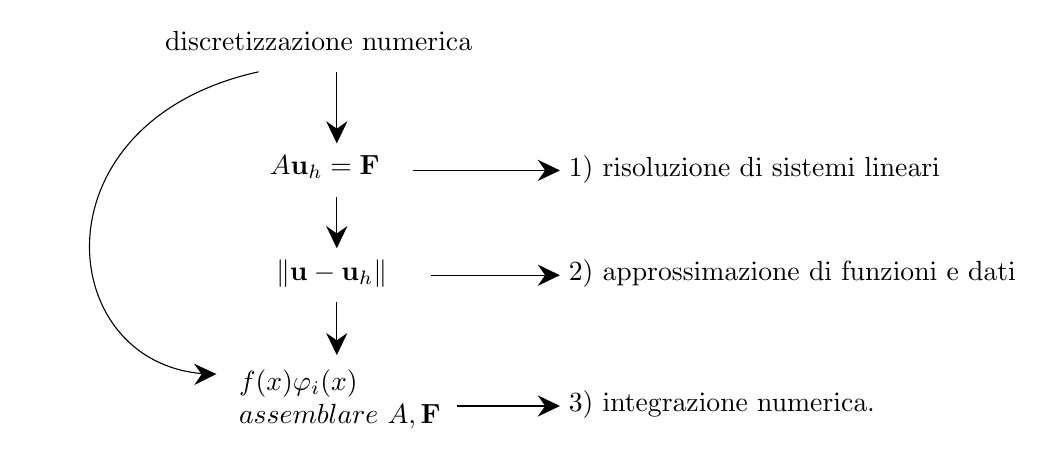
\begin{tikzpicture}[x=0.75pt,y=0.75pt,yscale=-1,xscale=1]
	%uncomment if require: \path (0,224); %set diagram left start at 0, and has height of 224


	% Text Node
	\draw (154,71.9) node [anchor=north west][inner sep=0.75pt]    {$A\mathbf{u}_{h} =\mathbf{F}$};
	% Text Node
	\draw (103.5,12) node [anchor=north west][inner sep=0.75pt]   [align=left] {discretizzazione numerica};
	% Text Node
	\draw (298,72) node [anchor=north west][inner sep=0.75pt]   [align=left] {1) risoluzione di sistemi lineari};
	% Text Node
	\draw (157,122.4) node [anchor=north west][inner sep=0.75pt]    {$\Vert \mathbf{u} -\mathbf{u}_{h}\Vert$};
	% Text Node
	\draw (298,122.5) node [anchor=north west][inner sep=0.75pt]   [align=left] {2) approssimazione di funzioni e dati};
	% Text Node
	\draw (132.5,173.9) node [anchor=north west][inner sep=0.75pt]    {$ \begin{array}{l}
	\bigintssss f(x) \varphi _{i}(x) \dx\\
	\text{assemblare} \ A,\mathbf{F}
	\end{array}$};
	% Text Node
	\draw (298,185.5) node [anchor=north west][inner sep=0.75pt]   [align=left] {3) integrazione numerica.};
	% Connection
	\draw    (187.5,33) -- (187.5,64.5) ;
	\draw [shift={(187.5,67.5)}, rotate = 270] [fill={rgb, 255:red, 0; green, 0; blue, 0 }  ][line width=0.08]  [draw opacity=0] (10.72,-5.15) -- (0,0) -- (10.72,5.15) -- (7.12,0) -- cycle    ;
	% Connection
	\draw    (187.5,93.5) -- (187.5,115) ;
	\draw [shift={(187.5,118)}, rotate = 270] [fill={rgb, 255:red, 0; green, 0; blue, 0 }  ][line width=0.08]  [draw opacity=0] (10.72,-5.15) -- (0,0) -- (10.72,5.15) -- (7.12,0) -- cycle    ;
	% Connection
	\draw    (149.81,33) .. controls (38.83,57.56) and (51.25,177.33) .. (127.18,178.61) ;
	\draw [shift={(129.5,178.61)}, rotate = 539.1600000000001] [fill={rgb, 255:red, 0; green, 0; blue, 0 }  ][line width=0.08]  [draw opacity=0] (10.72,-5.15) -- (0,0) -- (10.72,5.15) -- (7.12,0) -- cycle    ;
	% Connection
	\draw    (224,80.5) -- (292,80.5) ;
	\draw [shift={(295,80.5)}, rotate = 180] [fill={rgb, 255:red, 0; green, 0; blue, 0 }  ][line width=0.08]  [draw opacity=0] (10.72,-5.15) -- (0,0) -- (10.72,5.15) -- (7.12,0) -- cycle    ;
	% Connection
	\draw    (233,131) -- (292,131) ;
	\draw [shift={(295,131)}, rotate = 180] [fill={rgb, 255:red, 0; green, 0; blue, 0 }  ][line width=0.08]  [draw opacity=0] (10.72,-5.15) -- (0,0) -- (10.72,5.15) -- (7.12,0) -- cycle    ;
	% Connection
	\draw    (187.5,144) -- (187.5,166.5) ;
	\draw [shift={(187.5,169.5)}, rotate = 270] [fill={rgb, 255:red, 0; green, 0; blue, 0 }  ][line width=0.08]  [draw opacity=0] (10.72,-5.15) -- (0,0) -- (10.72,5.15) -- (7.12,0) -- cycle    ;
	% Connection
	\draw    (245.5,194) -- (292,194) ;
	\draw [shift={(295,194)}, rotate = 180] [fill={rgb, 255:red, 0; green, 0; blue, 0 }  ][line width=0.08]  [draw opacity=0] (10.72,-5.15) -- (0,0) -- (10.72,5.15) -- (7.12,0) -- cycle    ;

	\end{tikzpicture}
\end{figure}
\FloatBarrier

Aggiungiamo un ulteriore grado di complessità rispetto al problema proposto all'inizio del capitolo \ref{chap:introduzione}, cioè la variazione nel tempo oltre che nello spazio.
Invece di avere una corda fissata agli estremi, osserviamo una barra di metallo che riscaldiamo. Vogliamo modellizzare come varia la temperatura $u( x,t)$ in funzione dello spazio $x$ e del tempo $t$, assegnate la temperatura agli estremi, la temperatura all'istante iniziale e la sorgente termica.

Si può mostrare (ma non rientra nella nostra trattazione) che questo problema è modellato dall'\textit{equazione del calore}, abbinata ad opportune condizioni:
\begin{equation}\tag{PM}\label{eq:pm-calore}
\left\{\begin{array}{ l l l }
u_{t}( x,t) -u_{xx}( x,t) =f( x,t)  & x\in ( 0,1) ,\forall t & \text{(equazione del calore)}\\
u( 0,t) =0,\quad u( 1,t) =0 & \forall t >0 & \text{(condizioni ai limiti)}\\
u( x,0) =u_{0}(x) & \forall x\in ( a,b) & \text{(condizione iniziale).}
\end{array}\right.
\end{equation}
La funzione cercata $u( x,t)$ è la soluzione dell'equazione del calore.
Questa è un esempio di \textit{equazione differenziale}, che approfondiremo nel capitolo \ref{chap:edo}.
La risoluzione di questo tipo di equazione è uno dei principali motivi di interesse per l'approssimazione numerica di derivate.

Riscriviamo \eqref{eq:pm-calore} nel seguente modo, moltiplicando per una certa funzione $v=v(x)$ e integrando in $( 0,1)$:
\begin{equation*}
\int\nolimits ^{1}_{0}( u_{t} v-u_{xx} v) \dx=\int\nolimits ^{1}_{0} fv\dx.
\end{equation*}
Integriamo poi per parti il primo membro:
\begin{equation*}
\int\nolimits ^{1}_{0} u_{t} v\dx+\int\nolimits ^{1}_{0} u_{x} v_{x} \dx-[ u_{x} v]^{1}_{0} =\int\nolimits ^{1}_{0} fv\dx.
\end{equation*}
Come nel caso già affrontato in sezione \ref{sec:formulazione-debole}, $v$ è una funzione, in uno spazio ancora non definito, tale che $v(0) =0$, $v(1) =0$.
Si ha dunque:
\begin{equation*}
[ u_{x} v]^{1}_{0} =u_{x}( 1,t) v(1) -u_{x}( 0,t) v(0) =0.
\end{equation*}
Riscriviamo quindi il problema \eqref{eq:pm-calore}. $\forall t >0$,  trovare $u( x,t) \in V$ tale che:
\begin{equation*}\tag{PM'}\label{eq:pm1-calore}
\begin{cases}
\int\nolimits ^{1}_{0} u_{t}( x,t) v(x) \dx+\int\nolimits ^{1}_{0} u_{x}( x,t) v_{x}(x) \dx=\int\nolimits ^{1}_{0} f( x,t) v(x) \dx,\ \ \forall v\in V,\\
u( x,0) =u_{0}(x) ,
\end{cases}
\end{equation*}
dove
\begin{equation*}
V=\{
v:( 0,1)\rightarrow \mathbb{R} \ \text{tale che} \ v, v_{x} \in L^{2}( 0,1) ,\ v(0) =0,\ v(1) =0\}
\end{equation*}
è uno spazio infinito-dimensionale.
Vogliamo utilizzare invece uno spazio finito-dimensionale $V_{h} \subseteq V$, cioè tale che $\mathrm{dim}( V_{h}) =N_{h} < +\infty $.
Riscriviamo \eqref{eq:pm-calore} in $V_{h}$. $\forall t >0$ trovare $u_{h}( x,t) \in V_{h}$ tale che:
\begin{equation*}\tag{PN}\label{eq:pn-calore}
\begin{cases}
\int\nolimits ^{1}_{0}\frac{\partial u_{h}( x,t)}{\partial t} v_{h}(x) \dx+\int\nolimits ^{1}_{0}\frac{\partial u_{h}( x,t)}{\partial x}\frac{\partial v_{h}(x)}{\partial x} \dx=\int\nolimits ^{1}_{0} f( x,t) v_{h}(x) \dx,\ \ \forall v_{h} \in V_{h} ,\\
u_{h}( x,0) =u^{h}_{0}(x) ,
\end{cases}
\end{equation*}
dove $u^{h}_{0}(x) \in V_{h}$ è un'approssimazione di $u_{0}(x)$.

\textbf{Proprietà.}
\eqref{eq:pm-calore} è un sistema di equazioni differenziali del primo ordine della forma:
\begin{equation}
\begin{cases}
M\frac{\partial \mathbf{u}_{h}(t)}{\partial t} +A\mathbf{u}_{h}(t) =\mathbf{F}(t) ,\quad \forall t >0,\\
\mathbf{u}_{h}(0) =\mathbf{u}^{h}_{0} .
\end{cases}
\label{eq:sist-edp-pn}
\end{equation}


\textit{Dimostrazione.} Costruiamo una base per $V_{h}$
\begin{equation*}
V_{h} =\mathrm{span}\{\varphi _{1}(x) ,\varphi _{2}(x) ,\dotsc ,\varphi _{N_{h}}(x)\} ,
\end{equation*}
allora la soluzione $u_{h}( x,t)$ può essere scritta come combinazione lineare delle funzioni di base:
\begin{equation}
u_{h}( x,t) =\sum\limits ^{N_{h}}_{j=1} u_{j}(t) \varphi _{j}(x).
\label{eq:comb-lin-f-base}
\end{equation}
La dipendenza dal tempo è inclusa nei coefficienti $u_{j}(t)$.
Abbiamo pertanto costruito il vettore
\begin{equation*}
\mathbf{u}_{h}(t) =\begin{bmatrix}
u_{1}(t)\\
u_{2}(t)\\
\vdots \\
u_{N_{h}}(t)
\end{bmatrix} \in \mathbb{R}^{N_{h}} .
\end{equation*}
Riscriviamo (PN) utilizzando \eqref{eq:comb-lin-f-base} e otteniamo
\begin{gather*}
\int\nolimits ^{1}_{0}\frac{\partial }{\partial t}\left(\sum\limits ^{N_{h}}_{j=1} u_{j}(t) \varphi _{j}(x)\right) \varphi _{i}(x) \dx+\int\nolimits ^{1}_{0}\frac{\partial }{\partial x}\left[\sum\limits ^{N_{h}}_{j=1} u_{j}(t) \varphi _{j}(x)\right]\frac{\partial }{\partial x} \varphi _{i}(x) \dx=\\
=\int\nolimits ^{1}_{0} f( x,t) \varphi _{i}(x) \dx,\ \ \forall i=1,\dotsc ,N_{h}.
\end{gather*}
Usando la linearità e uno scambio tra derivata e integrale (possibile perché le due variabili coinvolte sono distinte), possiamo riorganizzare per ottenere:
\begin{gather*}
\sum\limits ^{N_{h}}_{j=1}\frac{\partial }{\partial t} u_{j}(t)\int\nolimits ^{1}_{0} \varphi _{j}(x) \varphi _{i}(x) \dx+\sum\limits ^{N_{h}}_{j=1} u_{j}(t)\int\nolimits ^{1}_{0}\frac{\partial }{\partial x} \varphi _{j}(x)\frac{\partial }{\partial x} \varphi _{i}(x) \dx=\\
=\int\nolimits ^{1}_{0} f( x,t) \varphi _{i}(x) \dx,\ \ \forall i=1,\dotsc ,N_{h} .
\end{gather*}
Definiamo ora la \textbf{matrice di massa}\index{matrice!di massa}
\begin{equation*}
M\in \mathbb{R}^{N_{h} \times N_{h}} ,\quad M_{ij} \coloneqq \int\nolimits ^{1}_{0} \varphi _{j}(x) \varphi _{i}(x) \dx,\quad \forall i,j=1,\dotsc ,N_{h} ,
\end{equation*}
e la matrice \textbf{matrice di rigidezza}\index{matrice!di rigidezza} (o \textit{stiffness matrix})
\begin{equation*}
A\in \mathbb{R}^{N_{h} \times N_{h}} ,\quad A_{ij} \coloneqq \int\nolimits ^{1}_{0}\frac{\partial }{\partial x} \varphi _{j}(x)\frac{\partial }{\partial x} \varphi _{i}(x) \dx,\quad \forall i,j=1,\dotsc ,N_{h} ,
\end{equation*}
quest'ultima è la stessa dell'equazione \eqref{eq:Au-F} presentata a inizio corso.
Infine definiamo il vettore
\begin{equation*}
\mathbf{F} \in \mathbb{R}^{N_{h}} ,\quad F_{i} =\int\nolimits ^{1}_{0} f( x,t) \varphi _{i}(x) \dx,\quad \forall i=1,\dotsc ,N_{h} .
\end{equation*}
Con queste definizioni possiamo riscrivere
\begin{equation*}\tag{EDO}
\begin{cases}
M\frac{\mathbf{\partial u}_{h}}{\partial t} +A\mathbf{u}_{h}(t) =\mathbf{F}(t) ,\quad \forall t >0,\\
\mathbf{u}_{h}(0) =\mathbf{u}^{h}_{0} .
\end{cases}
\end{equation*}
Per procedere alla risoluzione di questo \textit{problema non stazionario} avremo bisogno di far risolvere al calcolatore:
\begin{enumerate}
\item sistemi di EDO (Equazioni Differenziali Ordinarie),
\item sistemi di Equazioni Non Lineari.
\end{enumerate}

\section{Approssimazione di derivate}
Sia $f:[ a,b]\rightarrow \mathbb{R}$ derivabile con continuità e sia $\overline{x} \in ( a,b)$. Vogliamo approssimare $f'(\overline{x})$. Per definizione la derivata di $f$ in $\overline{x}$ è
\begin{equation*}
f'(\overline{x}) \coloneqq \lim _{h\rightarrow 0}\frac{f(\overline{x} +h) -f(\overline{x})}{h} ,
\end{equation*}
ma a livello numerico l'operazione di limite è ovviamente impossibile, e dovrà essere approssimata con $h$ piccoli.
Definiamo quindi la \textbf{differenza finita in avanti}\index{differenza finita!in avanti}:
\begin{equation}
f'(\overline{x}) \approx ( \delta _{+} f)(\overline{x}) :=\frac{f(\overline{x} +h) -f(\overline{x})}{h}.
\label{eq:diff-fin-avanti}
\end{equation}
La \textbf{differenza finita all'indietro}\index{differenza finita!all'indietro}:
\begin{equation}
f'(\overline{x}) \approx ( \delta _{-} f)(\overline{x}) :=\frac{f(\overline{x}) -f(\overline{x} -h)}{h}.
\label{eq:diff-fin-indietro}
\end{equation}
Infine, la media tra le due è detta \textbf{differenza finita centrata}\index{differenza finita!centrata}:
\begin{equation}
f'(\overline{x}) \approx ( \delta f)(\overline{x}) :=\frac{f(\overline{x} +h) -f(\overline{x} -h)}{2h}.
\label{eq:diff-fin-centrata}
\end{equation}

\begin{figure}[htpb]
	\centering
	\tikzset{every picture/.style={line width=0.75pt}} %set default line width to 0.75pt

	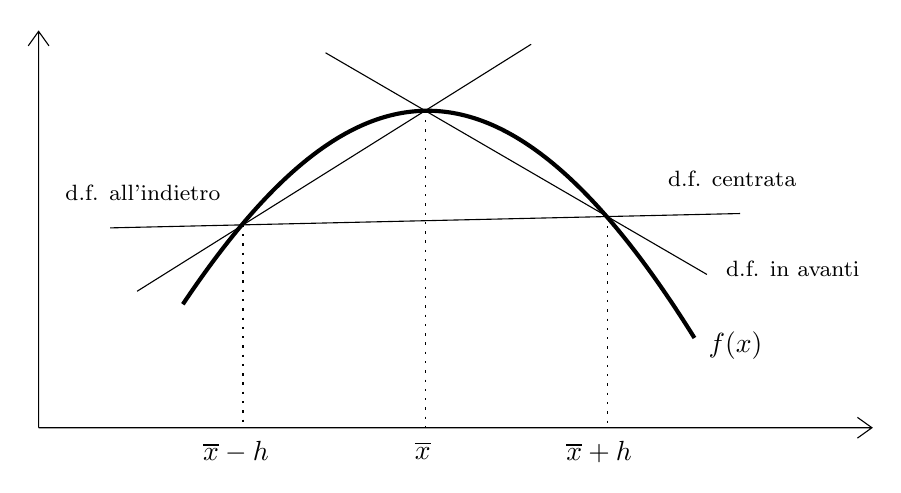
\begin{tikzpicture}[x=0.75pt,y=0.75pt,yscale=-1,xscale=1]
	%uncomment if require: \path (0,241); %set diagram left start at 0, and has height of 241

	%Shape: Axis 2D [id:dp2911281265961927]
	\draw  (116,210.5) -- (517.5,210.5)(116,19.5) -- (116,210.5) -- cycle (510.5,205.5) -- (517.5,210.5) -- (510.5,215.5) (111,26.5) -- (116,19.5) -- (121,26.5)  ;
	%Curve Lines [id:da2327769552172385]
	\draw [line width=1.5]    (185.5,151) .. controls (267,29.25) and (339.5,18.75) .. (432,167.25) ;
	%Straight Lines [id:da26722727505862176]
	\draw    (150.5,114.21) -- (454,107.29) ;
	%Straight Lines [id:da7308002840108798]
	\draw  [dash pattern={on 0.84pt off 2.51pt}]  (214.5,112.75) -- (214.5,210.5) ;
	%Straight Lines [id:da9253807449227653]
	\draw  [dash pattern={on 0.84pt off 2.51pt}]  (390,108.75) -- (390,210.5) ;
	%Straight Lines [id:da2972221464084601]
	\draw    (163.45,144.75) -- (353.3,25.75) ;
	%Straight Lines [id:da5117517681802604]
	\draw    (254.25,29.85) -- (438,136.65) ;
	%Straight Lines [id:da39389381197973306]
	\draw  [dash pattern={on 0.84pt off 2.51pt}]  (302.25,57.75) -- (302.25,210.5) ;

	% Text Node
	\draw (296,215.9) node [anchor=north west][inner sep=0.75pt]    {$\overline{x}$};
	% Text Node
	\draw (369,215.9) node [anchor=north west][inner sep=0.75pt]    {$\overline{x} +h$};
	% Text Node
	\draw (194,215.9) node [anchor=north west][inner sep=0.75pt]    {$\overline{x} -h$};
	% Text Node
	\draw (437.5,162.9) node [anchor=north west][inner sep=0.75pt]    {$f(x)$};
	% Text Node
	\draw (446,129) node [anchor=north west][inner sep=0.75pt]   [align=left] {{\footnotesize d.f. in avanti}};
	% Text Node
	\draw (127.67,92.5) node [anchor=north west][inner sep=0.75pt]  [font=\footnotesize] [align=left] {d.f. all'indietro};
	% Text Node
	\draw (418,85.5) node [anchor=north west][inner sep=0.75pt]   [align=left] {{\footnotesize d.f. centrata}};
	\end{tikzpicture}
	\caption{Intuizione grafica delle differenze all'indietro, centrate e in avanti con passo $h$.}
\end{figure}

\subsection{Errore di approssimazione delle derivate}

Supponiamo $f\in C^{2}(( a,b))$.
Possiamo sviluppare $f$ in serie di Taylor:
\begin{equation}
f(\overline{x} +h) =f(\overline{x}) +hf'(\overline{x}) +\frac{h^{2}}{2} f''( \xi ) ,\quad \xi \in (\overline{x} ,\overline{x} +h).
\label{eq:derivata-avanti}
\end{equation}
Analogamente, scrivendo l'espressione in $\overline{x} -h$:
\begin{equation}
f(\overline{x} -h) =f(\overline{x}) -hf'(\overline{x}) +\frac{h^{2}}{2} f''( \eta ) ,\quad \eta \in (\overline{x} -h,\overline{x}).
\label{eq:derivata-indietro}
\end{equation}
Possiamo riscrivere \eqref{eq:derivata-avanti} ottenendo l'errore di approssimazione:
\begin{align*}
\underbrace{\frac{f(\overline{x} +h) -f(\overline{x})}{h}}_{( \delta _{+} f)(\overline{x})} -f'(\overline{x}) & =\frac{h}{2} f''( \xi )\\
( \delta _{+} f)(\overline{x}) -f'(\overline{x}) & =\frac{h}{2} f''( \xi )\\
E^{+}(\overline{x}) & =\frac{h}{2} f''( \xi )
\end{align*}
e limitare superiormente questo errore:
\begin{align*}
 \left| E^{+}(\overline{x})\right| \leqslant \frac{h}{2}| f''( \xi )| \leqslant \frac{h}{2}\underbrace{\Vert f''(x)\Vert _{\infty }}_{\leqslant C} .
\end{align*}
Analogamente per \eqref{eq:derivata-indietro}:
\begin{align*}
\underbrace{\frac{f(\overline{x}) -f(\overline{x} -h)}{h}}_{( \delta _{-} f)(\overline{x})} -f'(\overline{x}) & =-\frac{h}{2} f''( \xi )\\
( \delta _{-} f)(\overline{x}) -f'(\overline{x}) & =-\frac{h}{2} f''( \xi )\\
E^{-}(\overline{x}) & =-\frac{h}{2} f''( \xi ) \\
\Rightarrow \ \ \left| E^{-}(\overline{x})\right| &\leqslant \frac{h}{2}| f''( \xi )| \leqslant \frac{h}{2}\underbrace{\Vert f''(x)\Vert _{\infty }}_{\leqslant C} .
\end{align*}
L'errore è quindi un infinitesimo di ordine $1$ rispetto ad $h$.

% \textit{[Lezione 16 (27-04-2020)]}

Per stimare l'errore della differenza finita centrata, supponiamo $f\in C^{3}(( a,b))$ e sviluppiamo $f$ in serie di Taylor fino all'ordine 3:
\begin{gather}
f(\overline{x} +h) =f(\overline{x}) +hf'(\overline{x}) +\frac{h^{2}}{2} f''(\overline{x}) +\frac{h^{3}}{6} f'''( \xi ) ,\quad \xi \in (\overline{x} ,\overline{x} +h) \label{eq:derivata-avanti2}\\
f(\overline{x} -h) =f(\overline{x}) -hf'(\overline{x}) +\frac{h^{2}}{2} f''(\overline{x}) -\frac{h^{3}}{6} f'''( \eta ) ,\quad \eta \in (\overline{x} -h,\overline{x}) \label{eq:derivata-indietro2}
\end{gather}
sottraiamo \eqref{eq:derivata-avanti2} e \eqref{eq:derivata-indietro2} membro a membro:
\begin{equation*}
f(\overline{x} +h) -f(\overline{x} -h) =2hf'(\overline{x}) +\frac{h^{3}}{6}[ f'''( \xi ) +f'''( \eta )].
\end{equation*}
Dividendo per $2h$:
\begin{align*}
\underbrace{\frac{f(\overline{x} +h) -f(\overline{x} -h)}{2h}}_{( \delta f)(\overline{x})} -f'(\overline{x}) & =\frac{h^{2}}{12}[ f'''( \xi ) +f'''( \eta )]\\
( \delta f)(\overline{x}) -f'(\overline{x}) & =\frac{h^{2}}{12}[ f'''( \xi ) +f'''( \eta )]\\
E(\overline{x}) & =\frac{h^{2}}{12}[ f'''( \xi ) +f'''( \eta )].
\end{align*}
Prendendo la norma infinito:
\begin{gather*}
\Vert f'''( \xi )\Vert _{\infty } \leqslant \max_{x\in ( a,b)}| f'''(x)| =:\Vert f'''(x)\Vert _{\infty } ,\\
\Vert f'''( \eta )\Vert _{\infty } \leqslant \max_{x\in ( a,b)}| f'''(x)| =:\Vert f'''(x)\Vert _{\infty } ,\\
\Rightarrow | E(\overline{x})| \leqslant \frac{h^{2}}{6}\Vert f'''(x)\Vert _{\infty } .
\end{gather*}
Abbiamo guadagnato un ulteriore ordine di infinitesimo con le differenze centrate.
Più l'ordine di infinitesimo è alto, migliore è l'approssimazione, poiché $h \ll 1$ e quindi tende a zero aumentando il suo esponente.

\textit{Osservazione.}

Supponiamo si voglia approssimare
\begin{equation*}
f'( x_{i}) ,\quad i=0,\dotsc ,n,\quad x_{i} =a+ih.
\end{equation*}
\begin{itemize}
\item Per approssimarla nei punti (nodi) interni $x_{1} \dotsc x_{n-1}$ possiamo usare le differenze finite in avanti, all'indietro o centrate, a piacere.
\item Per approssimarla in $x_{0}$ possiamo usare solo le differenze finite in avanti:
\begin{equation*}
f'( x_{0}) \approx \frac{f( x_{1}) -f( x_{2})}{h}.
\end{equation*}
\item Per approssimarla in in $x_{n}$ possiamo usare solo le differenze finite all'indietro:
\begin{equation*}
f'( x_{n}) \approx \frac{f( x_{n}) -f( x_{n-1})}{h}.
\end{equation*}
\end{itemize}

Si ha quindi meno accuratezza agli estremi.
Introducendo le \textbf{differenze finite generalizzate}\index{differenza finita!generalizzata}, facendo riferimento a sviluppi di Taylor di ordine superiore, è possibile raggiungere l'ordine di infinitesimo desiderato.

\section{Approssimazione della derivata seconda}
Sia $f\in C^{2}([ a,b])$.
Vogliamo approssimare $f''(\overline{x})$, $x\in ( a,b)$, utilizzando, come prima, gli sviluppi di Taylor.
\begin{figure}[htpb]
	\centering
	\tikzset{every picture/.style={line width=0.75pt}} %set default line width to 0.75pt

	\begin{tikzpicture}[x=0.75pt,y=0.75pt,yscale=-1,xscale=1]
	%uncomment if require: \path (0,206); %set diagram left start at 0, and has height of 206

	%Shape: Axis 2D [id:dp8810490010723286]
	\draw  (141,164.56) -- (455.5,164.56)(155.5,17.34) -- (155.5,176.34) (448.5,159.56) -- (455.5,164.56) -- (448.5,169.56) (150.5,24.34) -- (155.5,17.34) -- (160.5,24.34)  ;
	%Curve Lines [id:da2795883668655186]
	\draw [line width=1.5]    (191,95) .. controls (233.5,35.34) and (330.5,129.34) .. (398.5,72.34) ;
	%Straight Lines [id:da84886858102728]
	\draw  [dash pattern={on 0.84pt off 2.51pt}]  (191,95) -- (191,165.34) ;
	%Straight Lines [id:da6214095133668482]
	\draw  [dash pattern={on 0.84pt off 2.51pt}]  (398.5,72.34) -- (398.5,166.34) ;
	%Straight Lines [id:da7636614893230751]
	\draw  [dash pattern={on 0.84pt off 2.51pt}]  (301.5,86.34) -- (301.5,165.34) ;

	% Text Node
	\draw (186,170.4) node [anchor=north west][inner sep=0.75pt]    {$a$};
	% Text Node
	\draw (396,170.4) node [anchor=north west][inner sep=0.75pt]    {$b$};
	% Text Node
	\draw (296,170.4) node [anchor=north west][inner sep=0.75pt]    {$\overline{x}$};
	% Text Node
	\draw (218,51.4) node [anchor=north west][inner sep=0.75pt]    {$f(x)$};
	\end{tikzpicture}
\end{figure}
\FloatBarrier

Fissiamo $h >0$ e scriviamo, supponendo $f\in C^{4}([ a,b])$:
\begin{gather*}
f(\overline{x} +h) =f(\overline{x}) +hf'(\overline{x}) +\frac{h^{2}}{2} f''(\overline{x}) +\frac{h^{3}}{6} f'''(\overline{x}) +\frac{h^{4}}{24} f^{\text{(iv)}}( \xi )\\
f(\overline{x} -h) =f(\overline{x}) -hf'(\overline{x}) +\frac{h^{2}}{2} f''(\overline{x}) -\frac{h^{3}}{6} f'''(\overline{x}) +\frac{h^{4}}{24} f^{\text{(iv)}}( \eta ).
\end{gather*}
con $\xi \in (\overline{x} ,\overline{x} +h)$ e $\eta \in (\overline{x} -h,\overline{x})$.
Sommiamo ora membro a membro:
\begin{equation*}
f(\overline{x} +h) +f(\overline{x} -h) =2f(\overline{x}) +h^{2} f''(\overline{x}) +\frac{h^{4}}{24}\left[ f^{\text{(iv)}}( \xi ) +f^{\text{(iv)}}( \eta )\right].
\end{equation*}
Isolando $f''(\overline{x})$:
\begin{equation*}
f''(\overline{x}) =\frac{f(\overline{x} +h) +f(\overline{x} -h) -2f(\overline{x})}{h^{2}} -\frac{h^{2}}{24}\left[ f^{\text{(iv)}}( \xi ) +f^{\text{(iv)}}( \eta )\right].
\end{equation*}
Definiamo l'approssimazione di $f''$ troncando gli infinitesimi di ordine superiore ad 1:
\begin{equation*}
f''(\overline{x}) \approx \frac{f(\overline{x} +h) +f(\overline{x} -h) -2f(\overline{x})}{h^{2}}.
\end{equation*}
L'errore di approssimazione è quindi:
\begin{equation*}
E(\overline{x}) =-\frac{h^{2}}{24}\left[ f^{\text{(iv)}}( \xi ) +f^{\text{(iv)}}( \eta )\right].
\end{equation*}
Passando alla norma infinito, otteniamo:
\begin{equation*}
| E(\overline{x})| \leqslant -\frac{h^{2}}{12}\left\Vert f^{\text{(iv)}}(x)\right\Vert _{\infty }.
\end{equation*}
Si noti che questa espressione vale solo per i nodi interni.

%!TEX root = ../main.tex
\chapter{Risoluzione di Equazioni Differenziali Ordinarie}
\label{chap:edo}

In questo capitolo ci dedicheremo alle EDO, \textbf{equazioni differenziali ordinarie}\index{equazioni differenziali ordinarie}, ovvero equazioni dalla forma generale:
\begin{equation*}
	F\left(x,y,y',y'',\cdots,y^{(n)} \right) = 0,
\end{equation*}
dove quindi sono coinvolte le derivate di $y$, la funzione incognita da determinare, ed eventualmente la variabile $x$, cioè l'argomento della $y$.

Queste equazioni sono importantissime, perché consentono di descrivere in modo molto accurato tantissimi fenomeni fisici, anche se in realtà questi si descrivono più propriamente con le EDP, \textbf{equazioni alle derivate parziali}\index{equazioni alle derivate parziali}.
Nelle EDP non c'è dipendenza da una sola variabile, ma da più variabili, quindi naturalmente si potrà derivare la funzione incognita rispetto a ciascuna delle variabili, eventualmente più volte.
Tipicamente quando la dipendenza è da una sola variabile essa si può interpretare come un tempo o uno spazio. Quando però si vuole studiare l'evoluzione nel tempo di un sistema in 3D è chiaro che servono $3+1$ variabili, quindi una EDP.
Un aspetto interessante è che a volte la risoluzione delle EDP può essere ridotta a una EDO, per cui anche lo studio che affronteremo adesso sarà fondamentale per la modellistica fisica e le simulazioni numeriche.

\textit{Esempio.}
Supponiamo di avere una popolazione di batteri in un ambiente limitato nel quale non possono convivere più di $B$ batteri contemporaneamente. Supponiamo inoltre che all'istante in cui inizia l'esperimento, il numero di batteri sia $y_{0} \ll B$ e che il fattore di crescita dei batteri sia pari a una costante $r >0$. Come cambia nel tempo il numero di batteri?

Per scrivere un modello matematico di questo problema, dobbiamo anzitutto definire la quantità di interesse: sia $y(t)$ il numero di batteri all'istante $t$.

I dati sono:
\begin{itemize}
\item $y(0) =y_{0}$, la quantità di batteri all'istante iniziale $t=0$;
\item $r$, il fattore di crescita;
\item $B$, il numero massimo di batteri che possono coesistere.
\end{itemize}
Supponiamo $y \in C^{1} $: se a un certo punto $y(t) =B$, la derivata di $y(t)$ si deve annullare in quel punto.

Scriviamo ora il modello:
\begin{equation*}
\begin{cases}
\frac{\dy(t)}{\dt} =r\ y(t)\left( 1-\frac{y(t)}{B}\right)\\
y(0) =y_{0}.
\end{cases}
\end{equation*}
Esso è un esempio di \textbf{equazione funzionale}\index{equazione!funzionale}, in quanto i suoi elementi, inclusa l'incognita $y(t)$, sono funzioni e non quantità algebriche.
In particolare, è un'\textit{equazione differenziale ordinaria} (EDO), poiché presenta operazioni di derivazione.
\textit{Ordinaria} significa che non presenta derivate parziali.
L'\textit{ordine} di tale equazione è invece il più alto grado di derivazione presente.
In particolare, ci concentreremo sulle equazioni differenziali di primo ordine.

Supponiamo ora di avere due popolazioni di batteri distinte e in competizione tra loro. Indichiamo con $y_{1}(t)$ e $y_{2}(t)$ il numero di batteri rispettivamente della prima e della seconda popolazione. In questo caso il modello matematico diventa:
\begin{equation*}
\begin{cases}
\frac{\dy_{1}}{\dt} =r_{1} y_{1}( 1-b_{1} y_{1} -d_{2} y_{2})\\
\frac{\dy_{2}}{\dt} =r_{2} y_{2}( 1-b_{2} y_{2} -d_{1} y_{1})\\
y_{1}(0) =y^{0}_{1}\\
y_{2}(0) =y^{0}_{2}
\end{cases}
\end{equation*}
dove
\begin{itemize}
\item $r_{1} ,r_{2}$ sono i fattori di crescita delle due popolazioni
\item $b_{1} ,b_{2}$ sono fattori legati alla disponibilità di nutrienti, e quindi alla sopravvivenza delle singole popolazioni
\item $d_{1} ,d_{2}$ sono fattori che governano le interazioni, cioè la competizione, tra le due popolazioni.
\end{itemize}

La soluzione è della forma
\begin{equation*}
\y(t) =\begin{pmatrix}
y_{1}(t)\\
y_{2}(t)
\end{pmatrix}.
\end{equation*}

% \textit{[Lezione 17 (28-04-2020)]}
\section{Problema di Cauchy}
In generale, il problema matematico modello che vogliamo studiare si può così formulare:
Sia $I=[ t_{0} ,t_{0} +T]$ e $f:I\times \mathbb{R}\rightarrow \mathbb{R}$, vogliamo trovare $y(t) :I\rightarrow \mathbb{R}$ tale che
\begin{equation}
\tag{PC}
\begin{cases}
y'(t) =f( t,y(t))\\
y( t_{0}) =y_{0}
\end{cases} \quad t\in I
\label{eq:problema-di-cauchy}
\end{equation}
dove $y_{0} \in \mathbb{R}$ è assegnato.

\textit{Osservazione.}
Se la funzione $f$ è continua rispetto a $t$, possiamo integrare la prima equazione di \eqref{eq:problema-di-cauchy} tra $t_{0}$ e $t$ ottenendo la seguente formulazione:
\begin{equation*}
y(t) =y_{0} +\int\nolimits ^{t}_{t_{0}} f( \tau ,y( \tau )) \de\tau.
\end{equation*}
Ci interessa conoscere:
\begin{enumerate}
\item se \eqref{eq:problema-di-cauchy} ammette una sola soluzione;
\item la regolarità di questa soluzione;
\item se la soluzione sia stabile rispetto ai dati, ovvero se dipenda con continuità da essi.
\end{enumerate}

\begin{definition}
[Funzione lipschitziana]
\index{funzione!lipschitziana}
Una funzione $g:I\rightarrow \mathbb{R}$ è detta lipschitziana se esiste una costante $L$ tale che
\begin{equation*}
| g( x) -g( y)| \leqslant L| x-y| ,\ \ \forall x,y\in I.
\end{equation*}
Inoltre la costante migliore, cioè la più bassa possibile che rispetti la disuguaglianza, viene detta costante di Lipschitz.
\end{definition}

\begin{theorem}
[Esistenza della soluzione del \eqref{eq:problema-di-cauchy}]
\index{teorema!della soluzione del problema di cauchy}
Supponiamo che la funzione $f( \cdot ,\cdot )$ sia continua rispetto a entrambe le variabili, e che sia lipschitziana rispetto al secondo argomento.
Allora la soluzione del Problema di Cauchy \eqref{eq:problema-di-cauchy} esiste ed è unica, e inoltre $y\in C^{1}(I)$.
\label{thm:esistenza-unicita-PC}
\end{theorem}

Il teorema risponde ai primi due punti. Al fine di studiare il terzo punto, ovvero la stabilità di \eqref{eq:problema-di-cauchy}, consideriamo il seguente problema perturbato:
\begin{equation*}
(\widetilde{\text{PC}}) \ \begin{cases}
z'(t) =f( t,z(t)) +\delta (t)\\
z(0) =y_{0} +\delta _{0}
\end{cases} \quad t\in I
\end{equation*}
dove $\delta _{0} \in \mathbb{R}$ e $\delta (t)$ è una funzione continua in $I$. Vogliamo caratterizzare la sensibilità di $z(t)$ alle perturbazioni $\delta _{0}$ e $\delta (t)$. Questo è il concetto di stabilità secondo Lyapunov.

\begin{definition}
[Stabilità secondo Lyapunov]
\index{stabilità!secondo Lyapunov}
Sia $I=[ t_{0} ,t_{0} +T]$ un intervallo limitato $( T< +\infty )$.
Diciamo che \eqref{eq:problema-di-cauchy} è stabile secondo Lyapunov se per ogni perturbazione $( \delta _{0} ,\delta (t))$ tale che
\begin{equation*}
| \delta _{0}| < \varepsilon ,\quad | \delta (t)| < \varepsilon ,\quad \forall t\in I,\quad \varepsilon  >0,
\end{equation*}
con $\varepsilon $ sufficientemente piccolo da garantire che $(\widetilde{\text{PC}})$ ammetta una e una sola soluzione, allora esiste $c >0$, indipendente da $\varepsilon $, tale che
\begin{equation}
| y(t) -z(t)| < c\ \varepsilon ,\quad \forall t\in I.
\label{eq:stabilita-lyapunov}
\end{equation}
\end{definition}

\begin{definition}
[Stabilità asintotica]
\index{stabilità!asintotica}
Sia $I$ un intervallo superiormente illimitato.
Si dice che \eqref{eq:problema-di-cauchy} è asintoticamente stabile se vale \eqref{eq:stabilita-lyapunov} e inoltre
\begin{equation*}
\lim _{t\rightarrow \infty }| y(t) -z(t)| =0
\end{equation*}
purché $| \delta (t)| \rightarrow 0$ per $t\rightarrow \infty $.
\end{definition}

Enunciamo ora un lemma utile nella dimostrazione di risultati di stabilità.
\begin{lemma}
[Gronwall]
\index{lemma!di Gronwall}
Sia $p$ una funzione integrabile e non negativa sull'intervallo $[ t_{0} ,t_{0} +T]$ e siano $g$ e $\varphi $ due funzioni continue su $[ t_{0} ,t_{0} +T]$, con $g$ non decrescente. Allora
\begin{equation*}
\varphi (t) \leqslant g(t) +\int\nolimits ^{t}_{t_{0}} p(s) \varphi (s) \ds \ \ \Rightarrow \ \ \varphi (t) \leqslant g(t)\exp\left(\int\nolimits ^{t}_{t_{0}} p(s) \ds\right).
\end{equation*}
\end{lemma}

\begin{theorem}
[Stabilità]
\index{teorema!della stabilita}
Sia $f( \cdot ,\cdot )$ lipschitziana rispetto al secondo argomento. Allora \eqref{eq:problema-di-cauchy} è asintoticamente stabile.
\label{thm:stabilita-PC}
\end{theorem}

\textit{Dimostrazione.}
Sia $y(t)$ la soluzione di \eqref{eq:problema-di-cauchy} e sia $z(t)$ la soluzione di $(\widetilde{\text{PC}})$. Definiamo $w(t) =z(t) -y(t)$. Si ha, con $t\in I$:
\begin{equation*}
\begin{cases}
w'(t) =f( t,z(t)) +\delta (t) -f( t,y(t))\\
w( t_{0}) =\cancel{y_{0}} +\delta _{0} -\cancel{y_{0}}.
\end{cases}
\end{equation*}
Integriamo entrambi i membri della prima equazione tra $t_{0}$ e $t$:
\begin{align*}
\int\nolimits ^{t}_{t_{0}} w'(s) \ds & =\int\nolimits ^{t}_{t_{0}}[ f( s,z(s)) +\delta (s) -f( s,y(s))] \ds\\
w(t) -w( t_{0}) & =\int\nolimits ^{t}_{t_{0}}[ f( s,z(s)) -f( s,y(s))] \ds+\int\nolimits ^{t}_{t_{0}} \delta (s) \ds\\
w(t) & =\delta _{0} +\int\nolimits ^{t}_{t_{0}}[ f( s,z(s)) -f( s,y(s))] \ds+\int\nolimits ^{t}_{t_{0}} \delta (s) \ds
\end{align*}
Passiamo al modulo e otteniamo:
\begin{equation*}
| w(t)| \leqslant | \delta _{0}| +\int\nolimits ^{t}_{t_{0}}| f( s,z(s)) -f( s,y(s))| \ds+\int\nolimits ^{t}_{t_{0}}| \delta (s)| \ds.
\end{equation*}
Ricordando che $f$ è lipschitziana per ipotesi:
\begin{equation*}
| w(t)| \leqslant | \delta _{0}| +\int\nolimits ^{t}_{t_{0}} L| z(s) -y(s)| \ds+\int\nolimits ^{t}_{t_{0}}| \delta (s)| \ds.
\end{equation*}
Considerando che per definizione $z(s) -y(s) =:w(s)$:
\begin{equation*}
| w(t)| \leqslant | \delta _{0}| +L\int\nolimits ^{t}_{t_{0}}| w(s)| \ds+\int\nolimits ^{t}_{t_{0}}| \delta (s)| \ds,
\end{equation*}
quindi se $| \delta _{0}| < \varepsilon $ e $| \delta (s)| < \varepsilon $, $\forall t\in I$, possiamo riscriverlo come
\begin{align*}
| w(t)|  & \leqslant \varepsilon +L\int\nolimits ^{t}_{t_{0}}| w(s)| \ds+\int\nolimits ^{t}_{t_{0}} \varepsilon \ds\\
 & \leqslant \varepsilon ( 1+| t-t_{0}| ) +L\int\nolimits ^{t}_{t_{0}}| w(s)| \ds.
\end{align*}

Usando il lemma di Gronwall con $g(t) =\varepsilon ( 1+| t-t_{0}| )$ e $p(t) =L$, si ottiene:
\begin{align*}
| w(t)|  & \leqslant \varepsilon ( 1+| t-t_{0}| )\exp\left(\int\nolimits ^{t}_{t_{0}} L\ds\right)\\
 & \leqslant \varepsilon ( 1+| t-t_{0}| ) e^{L| t-t_{0}| }.
\end{align*}
Poiché $| t-t_{0}| \leqslant T$, si ha:
\begin{equation*}
| w(t)| \leqslant \varepsilon ( 1+T) e^{LT}.
\end{equation*}
Definendo $c \coloneqq ( 1+T) e^{LT}$, allora:
\begin{gather*}
| w(t)| \leqslant c \ \varepsilon.
\qed
\end{gather*}
\begin{theorem}
[Buona posizione]
\index{teorema!della buona posizione}
Sotto le ipotesi del teorema \ref{thm:esistenza-unicita-PC} il \eqref{eq:problema-di-cauchy} è ben posto, cioè esiste un'unica soluzione $y(t) \in C^{1}(I)$ che dipende con continuità dai dati, ovvero è stabile secondo Lyapunov.
\end{theorem}

\textit{Osservazioni.}
\begin{itemize}
\item Dalla dimostrazione del teorema \ref{thm:stabilita-PC}, abbiamo mostrato che la costante di stabilità
\begin{equation*}
c=( 1+T) e^{LT}
\end{equation*}
cresce esponenzialmente all'aumentare di $T$, l'ampiezza dell'intervallo, ovvero il tempo di osservazione.
\item Per costruire i metodi numerici lavoreremo solo con \eqref{eq:problema-di-cauchy} che sono ben posti.
\end{itemize}
\section{Metodi numerici a un passo}
Analizziamo ora quattro esempi di \textbf{metodi ad un passo}\index{metodo!ad un passo}. Ciò significa che, per calcolare la derivata a un certo $t_{n+1}$ utilizziamo solo informazioni che dipendono dal passo $t_{n}$.
Esistono anche metodi a più passi, o multistep, dove sfruttiamo più informazioni precedenti anziché solo quella immediatamente precedente.
Essi saranno l'oggetto della sezione \ref{sec:metodi-multistep}.

Sia $I=( t_{0} ,t_{0} +T)$, con $0< T< +\infty $, e sia data la funzione $f( \cdot ,\cdot ) :I\times \mathbb{R}\rightarrow \mathbb{R}$.
Ricordiamo la formulazione del modello di interesse, il problema di Cauchy:
\begin{equation*}
\tag{PC}
\begin{cases}
y'(t) =f( t,y(t))\\
y( t_{0}) =y_{0}
\end{cases} \quad t\in I.
\end{equation*}
Per risolvere numericamente il problema, seguiremo la seguente procedura:
\begin{enumerate}
\item Discretizziamo l'intervallo temporale $I$: fissiamo il passo di integrazione temporale $h >0$  e costruiamo i nodi di discretizzazione
\begin{equation*}
t_{n} =t_{0} +nh,\quad n=0,1,\dotsc ,N_{h}
\end{equation*}

dove $N_{h}$ è il massimo intero tale che $t_{N_{h}} =t_{0} +N_{h} h\leqslant t_{0} +T$.
\item Costruiamo un'approssimazione di $y( t_{n})$ per ogni nodo $t_{n}$. Anzitutto, \eqref{eq:problema-di-cauchy} soddisfa
\begin{equation*}
\begin{cases}
y'( t_{n}) =f( t_{n} ,y( t_{n}))\\
y( t_{0}) =y_{0}
\end{cases} \quad t\in I.
\end{equation*}
Definiamo
\begin{equation*}
u_{n} \approx y( t_{n}) ,\quad n=0,1,\dotsc ,N_{h}
\end{equation*}

e riscriviamo il \eqref{eq:problema-di-cauchy} approssimando numericamente la derivata.
Il modo che utilizziamo per approssimarla dà origine a diversi metodi numerici.
\end{enumerate}

\subsection{Metodo di Eulero Esplicito}
Analizziamo il metodo di \textbf{Eulero esplicito}\index{metodo!di Eulero esplicito} (o \textbf{Eulero in avanti}\index{metodo!di Eulero in avanti}), che abbrevieremo con \eqref{eq:eulero-avanti}.
Approssimando la derivata con la formula delle differenze finite in avanti (vedi \eqref{eq:diff-fin-avanti}) otteniamo:
\begin{equation*}
\frac{u_{n+1} -u_{n}}{h} =f( t_{n} ,u_{n}) ,\quad n=0,1,\dotsc ,N_{h} -1.
\end{equation*}

Dato che $u_{0} =y( t_{0}) =y_{0}$, calcoliamo gli $u_{n}$ nel seguente modo:
\begin{gather*}
u_{0}\rightarrow u_{1} =u_{0} +hf( t_{0} ,u_{0})\\
u_{1}\rightarrow u_{2} =u_{1} +hf( t_{1} ,u_{1})\\
\vdots \\
u_{n}\rightarrow u_{n+1} =u_{n} +hf( t_{n} ,u_{n}).
\end{gather*}

Pertanto otteniamo, per $n=0,1,\dotsc ,N_{h} -1$:
\begin{equation}\tag{EE}
\begin{cases}
u_{n+1} =u_{n} +hf( t_{n} ,u_{n})\\
u_{0} =y_{0}.
\end{cases}
\label{eq:eulero-avanti}
\end{equation}

\subsection{Metodo di Eulero Implicito}
Analizziamo il metodo di \textbf{Eulero implicito}\index{metodo!di Eulero implicito} (o \textbf{Eulero all'indietro}\index{metodo!di Eulero all'indietro}), che abbrevieremo con \eqref{eq:eulero-indietro}.
Approssimiamo ora la derivata con le differenze finite all'indietro (vedi \eqref{eq:diff-fin-indietro}).
Con conti analoghi troviamo, per $n=0,1,\dotsc ,N_{h} -1$:
\begin{equation}\tag{EI}
\begin{cases}
u_{n+1} =u_{n} +hf( t_{n+1} ,u_{n+1})\\
u_{0} =y_{0}.
\end{cases}
\label{eq:eulero-indietro}
\end{equation}

\textbf{NB.}
Per calcolare $u_{n+1}$ ad ogni passo bisognerà quindi risolvere un'equazione non lineare, a meno che $f( \cdot ,\cdot )$ non sia lineare nel secondo argomento.

\subsection{Metodo di Crank–Nicolson}
Analizziamo il metodo di \textbf{Crank-Nicolson}\index{metodo!di Crank-Nicolson} \eqref{eq:crank-nicolson}.
Scriviamo la media aritmetica dei metodi \eqref{eq:eulero-avanti} ed \eqref{eq:eulero-indietro}, sommando membro a membro:
\begin{equation*}
\begin{cases}
\frac{1}{2} u_{n+1} +\frac{1}{2} u_{n+1} =\frac{1}{2} u_{n} +\frac{1}{2} hf( t_{n+1} ,u_{n+1}) +\frac{1}{2} u_{n} +\frac{1}{2} hf( t_{n} ,u_{n})\\
u_{0} =y_{0}
\end{cases}
\end{equation*}
da cui si ottiene la forma del metodo di Crank-Nicolson:
\begin{equation}\tag{CN}
	\begin{cases}
	u_{n+1} =u_{n} +\frac{h}{2}[ f( t_{n+1} ,u_{n+1}) +f( t_{n} ,u_{n})]\\
	u_{0} =y_{0}
	\end{cases}
	\label{eq:crank-nicolson}
\end{equation}
per $n=0,1,\dotsc ,N_{h} -1$.

Notiamo che è un metodo implicito, in quanto compare $u_{n+1}$ da entrambe le parti dell'uguaglianza. Ciò significa che non abbiamo già \textit{pronto e impacchettato} il suo valore, ma dovremo risolvere l'equazione implicita per trovarlo. % "cotto e mangiato" era anche meglio :Kappa:

\textit{Osservazione.}
Il metodo di Crank-Nicolson si può ricavare anche partendo dalla formulazione integrale del \eqref{eq:problema-di-cauchy}: % è normale che pensi al partito comunista?
\begin{equation*}
y(t) =y_{0} +\int\nolimits ^{t}_{t_{0}} f( \tau ,y( \tau )) \de\tau ,\quad t\in I.
\end{equation*}
Scriviamo la formulazione integrale anche per i sottointervalli $( t_{n} ,t_{n+1})$:
\begin{align*}
\int\nolimits ^{t_{n+1}}_{t_{n}} y'( \tau ) \de\tau  & =\int\nolimits ^{t_{n+1}}_{t_{n}} f( \tau ,y( \tau )) \de\tau \\
y( t_{n+1}) -y( t_{n}) & =\int\nolimits ^{t_{n+1}}_{t_{n}} f( \tau ,y( \tau )) \de\tau \\
y( t_{n+1}) & =y( t_{n}) +\int\nolimits ^{t_{n+1}}_{t_{n}} f( \tau ,y( \tau )) \de\tau
\end{align*}
per poi approssimare l'integrale con la formula dei trapezi:
\begin{equation*}
\begin{cases}
u_{n+1} =u_{n} +\frac{h}{2}[ f( t_{n+1} ,u_{n+1}) +f( t_{n} ,u_{n})]\\
u_{0} =y_{0}
\end{cases} \quad n=0,1,\dotsc ,N_{h} -1.
\end{equation*}

\subsection{Metodo di Heun}
Analizziamo il metodo di \textbf{Heun}\index{metodo!di Heun}, che abbrevieremo con \eqref{eq:heun}.
Riprendiamo il metodo di \eqref{eq:crank-nicolson}:
\begin{equation*}\tag{CN}
\begin{cases}
u_{n+1} =u_{n} +\frac{h}{2}[ f( t_{n+1} ,u_{n+1}) +f( t_{n} ,u_{n})]\\
u_{0} =y_{0}.
\end{cases}
\end{equation*}
Nel membro destro, sostituiamo a $u_{n+1}$ una sua stima $\hat{u}_{n+1}$ che siamo in grado di calcolare.
Otteniamo quindi, per $n=0,1,\dotsc ,N_{h} -1$:
\begin{equation}\tag{H}
\begin{cases}
\hat{u}_{n+1} =u_{n} +hf( t_{n} ,u_{n})\\
u_{n+1} =u_{n} +\frac{h}{2}[ f( t_{n+1} ,\hat{u}_{n+1}) +f( t_{n} ,u_{n})]\\
u_{0} =y_{0}.
\end{cases}
\label{eq:heun}
\end{equation}
In questo modo, il metodo è diventato esplicito dato che non compare $u_{n+1}$.

% \textit{[Lezione 18 (04-05-2020)]}
\section{Analisi dei metodi a un passo}
Studiamo ora l'efficacia dei metodi a un passo e la loro convergenza.
Cerchiamo inoltre di capire quali metodi funzionano meglio per quali specifiche situazioni.

\subsection{Consistenza}
Osserviamo che ciascuno dei metodi visti può essere scritto nella seguente forma generale:
\begin{equation}
\begin{cases}
u_{n+1} =u_{n} +h\Phi [ t_{n} ,u_{n} ,f( t_{n} ,u_{n}) ;h] ,\quad n=0,1,\dotsc N_{h} -1\\
u_{0} =y_{0}
\end{cases}
\label{eq:forma-generale-1-passo}
\end{equation}
dove $\Phi ( \cdot ,\cdot ,\cdot ;\cdot )$ è detta \textit{funzione di incremento}.

\textit{Esempi.}
\begin{itemize}
\item Nel caso di \eqref{eq:eulero-avanti}:
\begin{equation*}
\Phi [ t_{n} ,u_{n} ,f( t_{n} ,u_{n}) ;h] =f( t_{n} ,u_{n}).
\end{equation*}
\item Nel caso di \eqref{eq:heun}:
\begin{equation*}
\Phi [ t_{n} ,u_{n} ,f( t_{n} ,u_{n}) ;h] =\frac{1}{2}[ f( t_{n+1} ,u_{n} +hf( t_{n} ,u_{n+1})) +f( t_{n} ,u_{n})].
\end{equation*}
\end{itemize}

Si ha che la soluzione esatta non soddisfa esattamente la soluzione numerica, ma è presente un residuo, una quantità che, se possibile, vogliamo far tendere a zero.
\begin{equation*}
\begin{cases}
y( t_{n+1}) =y( t_{n}) +h\Phi ( t_{n} ,y( t_{n}) ,f( t_{n} ,y( t_{n})) ;h) +\varepsilon _{n+1}\\
y( t_{0}) =y_{0}.
\end{cases}
\end{equation*}
Chiamo $\varepsilon _{n+1}$ il \textbf{residuo}\index{residuo} che si genera all'istante $t_{n+1}$. Esso ha la forma
\begin{equation*}
\varepsilon _{n+1} =h\ \tau _{n+1}(h) .
\end{equation*}
La quantità $\tau _{n+1}(h)$ è l'\textbf{errore di troncamento locale}\index{errore!di troncamento locale}. Definiamo anche l'\textbf{errore di troncamento globale}\index{errore!di troncamento globale} come segue:
\begin{equation*}
\tau (h) =\max_{0\leqslant n\leqslant N_{h} -1}| \tau _{n+1}(h)|.
\end{equation*}
Questi errori dipendono dal troncamento effettuato nell'approssimazione della funzione con gli sviluppi di Taylor.
\begin{definition}
Un metodo della forma \eqref{eq:forma-generale-1-passo} è detto \textbf{consistente}\index{metodo!consistente} se
\begin{equation*}
\lim _{h\rightarrow 0} \tau (h) =0.
\end{equation*}
Inoltre diciamo che il metodo della forma \eqref{eq:forma-generale-1-passo} ha ordine $p$ se $\tau (h) =O\left( h^{p}\right)$ per $h\rightarrow 0$.
\end{definition}

\subsection{Zero-stabilità}
Se il problema subisce una piccola perturbazione, cosa sappiamo dire della differenza tra le soluzioni numeriche con e senza perturbazione?

Consideriamo il metodo generale della forma \eqref{eq:forma-generale-1-passo} e perturbiamolo:
\begin{equation*}
\begin{cases}
z_{n+1} =z_{n} +h\Phi ( t_{n} ,z_{n} ,f( t_{n} ,z_{n}) ;h) +\delta _{n+1}\\
z_{0} =y_{0} + \delta _{0}
\end{cases} \quad \forall n=0,1,\dotsc N_{h} -1
\end{equation*}
dove $\delta _{n+1} ,n=0,\dotsc ,N_{h} -1$ e $\delta _{0}$ sono le perturbazioni.
\begin{definition}
[Zero-stabilità]
\index{zero-stabilità}
Il metodo numerico della forma \eqref{eq:forma-generale-1-passo} è $0$-stabile se esistono $h_{0}  >0, C >0, \varepsilon _{0}  >0$ tali che $\forall h\in ( 0,h_{0}]$ e $\forall \varepsilon \in ( 0,\varepsilon _{0}]$, se $| \delta _{n}| \leqslant \varepsilon ,0\leqslant n\leqslant N_{h}$, allora
\begin{equation*}
\left| u^{(h)}_{n} -z^{(h)}_{n}\right| \leqslant C\varepsilon ,\quad n=0,\dotsc ,N_{h}.
\end{equation*}
\end{definition}

Il nome zero-stabilità deriva dal fatto che se le perturbazioni distano meno di $\varepsilon $, le soluzioni sono controllate a meno di una costante $C$ che non dipende da $h$, per $h\rightarrow 0$.
Essa è una proprietà specifica del metodo numerico e non del problema di Cauchy (il quale è sempre stabile, grazie alla lipschitzianità di $f$).

La zero-stabilità studia il comportamento della soluzione in \textit{intervalli limitati} per $h\rightarrow 0$.
\subsection{Convergenza}
\begin{definition}
[Convergenza]
\index{convergenza}
Diciamo che un metodo è convergente se
\begin{equation*}
| y( t_{n}) -u_{n}| \leqslant C(h) ,\quad \forall n=0,\dotsc ,N_{h}
\end{equation*}
dove $C(h)$ è un infinitesimo rispetto ad $h$. In tal caso diciamo che il metodo è convergente con ordine $p$ se $C(h) =O\left( h^{p}\right)$.
\end{definition}
\begin{theorem}
Consideriamo un metodo della forma \eqref{eq:forma-generale-1-passo} che sia consistente. Allora
\begin{equation*}
\text{convergenza} \Leftrightarrow \text{zero-stabilità}.
\end{equation*}
\end{theorem}

\subsection{Convergenza di Eulero Esplicito}
Riportiamo nel dettaglio l’analisi di convergenza per il metodo di Eulero Esplicito. Per ogni $n=0,\dotsc ,N_{h}$ scriviamo l'errore come:
\begin{equation*}
e_{n+1} =y( t_{n+1}) -u_{n+1}.
\end{equation*}
Aggiungiamo e sottraiamo $\tilde{u}_{n+1}$:
\begin{equation*}
e_{n+1} =\underbrace{\left( y( t_{n+1}) -\tilde{u}_{n+1}\right)}_{\text{errore di consistenza}} +\underbrace{\left(\tilde{u}_{n+1} -u_{n+1}\right)}_{\text{effetto memoria}},
\end{equation*}
essendo
\begin{equation}
\tilde{u}_{n+1} =y( t_{n}) +hf( t_{n} ,y( t_{n}))
\label{eq:convergenza-ee-primo-passo}
\end{equation}
la soluzione ottenuta applicando un passo del metodo di Eulero Esplicito a partire dal dato iniziale $y_{n}$. Stiamo cercando di mantenere solo l'errore dovuto all'approssimazione della derivata e non all'effetto memoria.

\begin{figure}[htpb]
	\centering
	\tikzset{every picture/.style={line width=0.75pt}} %set default line width to 0.75pt

	\begin{tikzpicture}[x=0.75pt,y=0.75pt,yscale=-1,xscale=1]
	%uncomment if require: \path (0,266); %set diagram left start at 0, and has height of 266

	%Curve Lines [id:da034892312278599125]
	\draw    (105.5,166.38) .. controls (204.5,158.38) and (273.5,167.38) .. (372.5,18.38) ;
	%Straight Lines [id:da8785454944361366]
	\draw    (176.5,220.67) -- (176.5,229.33) ;
	%Straight Lines [id:da39528602977210503]
	\draw    (94,225) -- (491,225) ;
	\draw [shift={(494,225)}, rotate = 180] [fill={rgb, 255:red, 0; green, 0; blue, 0 }  ][line width=0.08]  [draw opacity=0] (10.72,-5.15) -- (0,0) -- (10.72,5.15) -- (7.12,0) -- cycle    ;
	%Straight Lines [id:da5584172062463073]
	\draw  [dash pattern={on 0.84pt off 2.51pt}]  (176.5,197.67) -- (344.33,171.83) ;
	\draw [shift={(344.33,171.83)}, rotate = 351.25] [color={rgb, 255:red, 0; green, 0; blue, 0 }  ][fill={rgb, 255:red, 0; green, 0; blue, 0 }  ][line width=0.75]      (0, 0) circle [x radius= 3.35, y radius= 3.35]   ;
	\draw [shift={(176.5,197.67)}, rotate = 351.25] [color={rgb, 255:red, 0; green, 0; blue, 0 }  ][fill={rgb, 255:red, 0; green, 0; blue, 0 }  ][line width=0.75]      (0, 0) circle [x radius= 3.35, y radius= 3.35]   ;
	%Straight Lines [id:da2873454849651973]
	\draw  [dash pattern={on 0.84pt off 2.51pt}]  (176.5,160.67) -- (344.33,134.83) ;
	\draw [shift={(344.33,134.83)}, rotate = 351.25] [color={rgb, 255:red, 0; green, 0; blue, 0 }  ][fill={rgb, 255:red, 0; green, 0; blue, 0 }  ][line width=0.75]      (0, 0) circle [x radius= 3.35, y radius= 3.35]   ;
	\draw [shift={(176.5,160.67)}, rotate = 351.25] [color={rgb, 255:red, 0; green, 0; blue, 0 }  ][fill={rgb, 255:red, 0; green, 0; blue, 0 }  ][line width=0.75]      (0, 0) circle [x radius= 3.35, y radius= 3.35]   ;
	%Shape: Circle [id:dp4537649989697854]
	\draw  [fill={rgb, 255:red, 0; green, 0; blue, 0 }  ,fill opacity=1 ] (342,58.17) .. controls (342,56.79) and (343.12,55.67) .. (344.5,55.67) .. controls (345.88,55.67) and (347,56.79) .. (347,58.17) .. controls (347,59.55) and (345.88,60.67) .. (344.5,60.67) .. controls (343.12,60.67) and (342,59.55) .. (342,58.17) -- cycle ;
	%Straight Lines [id:da8554308299700688]
	\draw    (344.5,221) -- (344.5,229.67) ;
	%Straight Lines [id:da6369204585664499]
	\draw    (344.5,62.67) -- (344.66,129.33) ;
	\draw [shift={(344.67,131.33)}, rotate = 269.86] [color={rgb, 255:red, 0; green, 0; blue, 0 }  ][line width=0.75]    (7.65,-3.43) .. controls (4.86,-1.61) and (2.31,-0.47) .. (0,0) .. controls (2.31,0.47) and (4.86,1.61) .. (7.65,3.43)   ;
	\draw [shift={(344.5,60.67)}, rotate = 89.86] [color={rgb, 255:red, 0; green, 0; blue, 0 }  ][line width=0.75]    (7.65,-3.43) .. controls (4.86,-1.61) and (2.31,-0.47) .. (0,0) .. controls (2.31,0.47) and (4.86,1.61) .. (7.65,3.43)   ;
	%Straight Lines [id:da6756464042840566]
	\draw    (344.33,141.33) -- (344.33,165.83) ;
	\draw [shift={(344.33,167.83)}, rotate = 270] [color={rgb, 255:red, 0; green, 0; blue, 0 }  ][line width=0.75]    (7.65,-3.43) .. controls (4.86,-1.61) and (2.31,-0.47) .. (0,0) .. controls (2.31,0.47) and (4.86,1.61) .. (7.65,3.43)   ;
	\draw [shift={(344.33,139.33)}, rotate = 90] [color={rgb, 255:red, 0; green, 0; blue, 0 }  ][line width=0.75]    (7.65,-3.43) .. controls (4.86,-1.61) and (2.31,-0.47) .. (0,0) .. controls (2.31,0.47) and (4.86,1.61) .. (7.65,3.43)   ;
	%Straight Lines [id:da9675193989338564]
	\draw    (465.5,60.17) -- (465.34,169.83) ;
	\draw [shift={(465.33,171.83)}, rotate = 270.08] [color={rgb, 255:red, 0; green, 0; blue, 0 }  ][line width=0.75]    (7.65,-3.43) .. controls (4.86,-1.61) and (2.31,-0.47) .. (0,0) .. controls (2.31,0.47) and (4.86,1.61) .. (7.65,3.43)   ;
	\draw [shift={(465.5,58.17)}, rotate = 90.08] [color={rgb, 255:red, 0; green, 0; blue, 0 }  ][line width=0.75]    (7.65,-3.43) .. controls (4.86,-1.61) and (2.31,-0.47) .. (0,0) .. controls (2.31,0.47) and (4.86,1.61) .. (7.65,3.43)   ;
	%Straight Lines [id:da8189986399115188]
	\draw  [dash pattern={on 0.84pt off 2.51pt}]  (344.33,171.83) -- (465.33,171.83) ;
	%Straight Lines [id:da4540415193091536]
	\draw  [dash pattern={on 0.84pt off 2.51pt}]  (344.5,58.17) -- (465.5,58.17) ;

	% Text Node
	\draw (331,231.4) node [anchor=north west][inner sep=0.75pt]    {$t_{n+1}$};
	% Text Node
	\draw (171,231.4) node [anchor=north west][inner sep=0.75pt]    {$t_{n}$};
	% Text Node
	\draw (354,176.73) node [anchor=north west][inner sep=0.75pt]    {$u_{n+1}$};
	% Text Node
	\draw (299.67,28.73) node [anchor=north west][inner sep=0.75pt]    {$y( t_{n+1})$};
	% Text Node
	\draw (153,132.4) node [anchor=north west][inner sep=0.75pt]    {$y( t_{n})$};
	% Text Node
	\draw (150,188.73) node [anchor=north west][inner sep=0.75pt]    {$u_{n}$};
	% Text Node
	\draw (269,86.4) node [anchor=north west][inner sep=0.75pt]    {$y(t)$};
	% Text Node
	\draw (354.67,149) node [anchor=north west][inner sep=0.75pt]  [font=\footnotesize] [align=left] {eff. memoria};
	% Text Node
	\draw (354.67,119.4) node [anchor=north west][inner sep=0.75pt]    {$\tilde{u}_{n+1}$};
	% Text Node
	\draw (470.67,107.4) node [anchor=north west][inner sep=0.75pt]    {$e_{n+1}$};
	\end{tikzpicture}
	\caption{Intuizione grafica del ruolo dell'errore di consistenza e dell'effetto memoria nell'analisi di convergenza del metodo di Eulero Esplicito.}
\end{figure}

Dobbiamo stimare separatamente questi due errori.
\begin{enumerate}
\item Stimiamo l'errore di consistenza $y( t_{n+1}) -\tilde{u}_{n+1}$.

Scriviamo lo sviluppo di Taylor di $y$:
\begin{equation*}
y( t_{n+1}) =y( t_{n}) +hy'( t_{n}) +\frac{h^{2}}{2} y''( \xi ) ,\quad \xi \in ( t_{n} ,t_{n+1})
\end{equation*}
e sostituiamola insieme a \eqref{eq:convergenza-ee-primo-passo}:
\begin{align*}
y( t_{n+1}) -\tilde{u}_{n+1} & =\cancel{y( t_{n})} +\cancel{hf( t_{n} ,y( t_{n}))} +\frac{h^{2}}{2} y''( \xi ) -\cancel{y( t_{n})} -\cancel{hf( t_{n} ,y( t_{n}))}\\
 & =\frac{h^{2}}{2} y''( \xi ) =h\tau _{n+1}(h).
\end{align*}
\item Stimiamo l'errore dovuto all'effetto memoria, $\tilde{u}_{n+1} -u_{n+1}$:
\begin{align*}
	\tilde{u}_{n+1}                        & =y( t_{n}) +hf( t_{n} ,y( t_{n}))                                                  &                           \\
	u_{n+1}                                & =u_{n} +hf( t_{n} ,u_{n})                                                          &                           \\
	\tilde{u}_{n+1} -u_{n+1}               & =\underbrace{y( t_{n}) -u_{n}}_{e_{n}} +h[ f( t_{n} ,y( t_{n})) -f( t_{n} ,u_{n})] & \text{(sottraiamo)}       \\
	\left| \tilde{u}_{n+1} -u_{n+1}\right| & \leqslant | e_{n}| +h| f( t_{n} ,y( t_{n})) -f( t_{n} ,u_{n})|                     & \text{(modulo)}           \\
	                                       & \leqslant | e_{n}| +hL\underbrace{| y( t_{n}) -u_{n}| }_{e_{n}}                    & \text{(lipschitzianità)} \\
	                                       & \leqslant ( 1+hL)| e_{n}|.                                                         &
\end{align*}
\end{enumerate}
Mettendo insieme le due stime troviamo:
\begin{equation*}
| e_{n+1}| \leqslant h\tau _{n+1}(h) +( 1+hL)| e_{n}|
\end{equation*}
che possiamo riscrivere come:
\begin{equation*}
\begin{aligned}
| e_{n+1}|  & \leqslant h\tau (h) +( 1+hL)| e_{n}| \\
 & \leqslant h\tau (h) +( 1+hL)[ h\tau (h) +( 1+hL)| e_{n-1}| ]\\
 & \vdots \ ( e_{0} =0)\\
 & \leqslant h\tau (h)\left[ 1+( 1+hL) +( 1+hL)^{2} +\cdots +( 1+hL)^{n}\right]\\
 & \leqslant h\tau (h)\sum\limits ^{n}_{k=0}( 1+hL)^{k}
\end{aligned}
\end{equation*}
ricordando che $\tau (h) =\frac{h}{2}\Vert y''(t)\Vert _{\infty }$.
Sfruttiamo ora l'espressione della serie geometrica
\begin{equation*}
\sum\limits ^{n}_{k=0} x^{k} =\frac{1-x^{k+1}}{1-x},
\end{equation*}
pertanto abbiamo che
\begin{align*}
| e_{n+1}|  & \leqslant h\tau (h)\left[\frac{1-( 1+hL)^{n+1}}{1-( 1+hL)}\right]\\
 & \leqslant \frac{\tau (h)}{L}\left[ -1+( 1+hL)^{n+1}\right]\\
 & \leqslant \frac{\left[ e^{( n+1) hL} -1\right]}{L} \tau (h)\\
 & \leqslant \frac{e^{TL}}{L} \tau (h),
\end{align*}
allora il metodo converge perché $\tau (h) =\frac{h}{2}\Vert y''(t)\Vert _{\infty }$ e:
\begin{equation*}
| e_{n+1}| \leqslant Ch,\quad C=\frac{e^{TL}}{2L}\Vert y''(t)\Vert _{\infty } ,\quad \forall n=0,\dotsc ,N_{h} -1.
\end{equation*}
L'ordine di convergenza è $1$. \textqed

% \textit{[Lezione 19 (5-05-2020)]}
Riassumiamo senza dimostrare i risultati di convergenza di tutti e quattro i metodi studiati.
\begin{theorem}
[Convergenza di \eqref{eq:eulero-avanti}, \eqref{eq:eulero-indietro}, \eqref{eq:crank-nicolson}, \eqref{eq:heun}]
Sia $y\in C^{2}(I)$ la soluzione del \eqref{eq:problema-di-cauchy}. Allora
\begin{gather*}
\max_{n=0,\dotsc ,N_{h}}\left| y( t_{n}) -u^{EE}_{n}\right| \leqslant C_{EE} h\\
\max_{n=0,\dotsc ,N_{h}}\left| y( t_{n}) -u^{EI}_{n}\right| \leqslant C_{EI} h
\end{gather*}
dove $C_{EE} =C_{EE}(\Vert y''(t)\Vert _{\infty } ,T)  >0$ e $C_{EI} =C_{EI}(\Vert y''(t)\Vert _{\infty } ,T)  >0$. Quindi i metodi di \eqref{eq:eulero-avanti} e \eqref{eq:eulero-indietro} convergono con ordine $1$ rispetto ad $h$.

Se invece $y\in C^{3}(I)$, allora
\begin{gather*}
\max_{n=0,\dotsc ,N_{h}}\left| y( t_{n}) -u^{CN}_{n}\right| \leqslant C_{CN} h^{2}\\
\max_{n=0,\dotsc ,N_{h}}\left| y( t_{n}) -u^{H}_{n}\right| \leqslant C_{H} h^{2}
\end{gather*}
dove $C_{CN} =C_{CN}(\Vert y'''(t)\Vert _{\infty } ,T)  >0$ e $C_{H} =C_{H}(\Vert y'''(t)\Vert _{\infty } ,T)  >0$. Quindi i metodi di \eqref{eq:crank-nicolson} e \eqref{eq:heun} convergono con ordine $2$ rispetto ad $h$.
\end{theorem}

\subsection{Assoluta stabilità}
Studiamo il comportamento dei metodi quando $h$ è fissato e $t_{n}\rightarrow \infty $: in tal caso, desideriamo che la soluzione numerica $u_{n}$ si mantenga \textit{vicina} a $y( t_{n})$. Questa caratteristica è nota come \textbf{assoluta stabilità}\index{assoluta stabilità}, o $\mathcal{A}$\textbf{-stabilità}\index{$\mathcal{A}$-stabilità}.

Per analizzare la stabilità su intervalli illimitati, considereremo il seguente \textit{problema modello}:
\begin{equation}\tag{PMod}
\begin{cases}
y'(t) =\lambda y(t) ,\quad t\in ( 0,+\infty )\\
y(0) =1
\end{cases}
\label{eq:problema-modello}
\end{equation}
con $\lambda \in \mathbb{C}$, la cui soluzione di è $y(t) =e^{\lambda t}$. Inoltre se $\Re ( \lambda ) < 0$, si ha che $$\lim\limits _{t\rightarrow +\infty }| y(t)| =0.$$

\fg[Comportamento di \eqref{eq:problema-modello}]{0.7}{fig-problema-modello}

Vorremmo dunque che anche la soluzione numerica tenda a zero, in modo da catturare il comportamento asintotico della soluzione vera.
\begin{definition}
[Assoluta stabilità]
\index{assoluta stabilità}
Diciamo che un metodo numerico per l'approssimazione di \eqref{eq:problema-modello} è assolutamente stabile se
\begin{equation}
| u_{n}| \rightarrow 0\quad \text{per} \quad t_{n}\rightarrow +\infty.
\end{equation}
\label{eq:assoluta-stabilita}
\end{definition}

\textit{Osservazione.}
Per $h$ fissato, la soluzione numerica $u_{n}$ dipende da $h$ e da $\lambda $. Possiamo quindi dare la seguente definizione.
\begin{definition}
[Regione di assoluta stabilità]
\index{regione di assoluta stabilità}
Definiamo $\mathcal{A}$ la regione di assoluta stabilità di un metodo numerico il seguente sottoinsieme del piano complesso:
$$\mathcal{A} =\{z=h\lambda \in \mathbb{C} \text{ tali che \eqref{eq:assoluta-stabilita} è soddisfatta}\}.$$
\end{definition}

\textbf{NB.}
Poiché $h >0$ e $\Re ( \lambda ) < 0$ per ipotesi, sicuramente $\mathcal{A} \subseteq \mathbb{C}^{-}$.

\begin{definition}
[$\mathcal{A}$-stabilità]
\index{$\mathcal{A}$-stabilità}
Un metodo numerico è $\mathcal{A}$-stabile se $\mathcal{A} \cap \mathbb{C}^{-} =\mathbb{C}^{-}$, ovvero se per qualsiasi $\lambda \in \mathbb{C}^{-}$ la condizione \eqref{eq:assoluta-stabilita} è soddisfatta incondizionatamente rispetto ad $h$.
\end{definition}

\subsection{Stabilità di Eulero Esplicito}
Il metodo di Eulero esplicito applicato al problema modello \eqref{eq:problema-modello} diventa:
\begin{equation*}
\begin{cases}
u_{n+1} =u_{n} +h\underbrace{\lambda u_{n}}_{f( t_{n} ,u_{n})} \quad n=0,1,2,\dotsc \\
u_{0} =1.
\end{cases}
\end{equation*}
Quindi otteniamo $u_{n+1} =( 1+h\lambda ) u_{n}$, cioè, ricorsivamente:
\begin{align*}
u_{n+1} & =( 1+h\lambda ) u_{n}\\
 & =( 1+h\lambda )( 1+h\lambda ) u_{n-1}\\
 & \vdots \\
 & =( 1+h\lambda )^{n+1} u_{0}\\
 & =( 1+h\lambda )^{n+1}.
\end{align*}
Abbiamo quindi mostrato che il metodo di \eqref{eq:eulero-avanti} utilizzato per approssimare \eqref{eq:problema-modello} ha la seguente forma:
\begin{equation*}
\begin{cases}
u_{n} =( 1+h\lambda )^{n} \quad n=0,1,2,\dotsc \\
u_{0} =1.
\end{cases}
\end{equation*}
Dalla definizione di assoluta stabilità si ha che:
\begin{align}
\lim _{t_{n}\rightarrow +\infty }| u_{n}| =0 \quad  & \Leftrightarrow \quad\lim _{t_{n}\rightarrow +\infty }\left| ( 1+h\lambda )^{n}\right| =0\Leftrightarrow | 1+h\lambda | < 1 \\
													& \Leftrightarrow \quad h\lambda \in \mathbb{C}^{-} \ \text{e} \ 0< h< \frac{-2\Re ( \lambda )}{| \lambda | ^{2}}.
\label{eq:A-stab-ee}
\end{align}

\begin{figure}[htpb]
	\centering
	\tikzset{
	pattern size/.store in=\mcSize,
	pattern size = 5pt,
	pattern thickness/.store in=\mcThickness,
	pattern thickness = 0.3pt,
	pattern radius/.store in=\mcRadius,
	pattern radius = 1pt}
	\makeatletter
	\pgfutil@ifundefined{pgf@pattern@name@_abw8ptezs}{
	\pgfdeclarepatternformonly[\mcThickness,\mcSize]{_abw8ptezs}
	{\pgfqpoint{0pt}{-\mcThickness}}
	{\pgfpoint{\mcSize}{\mcSize}}
	{\pgfpoint{\mcSize}{\mcSize}}
	{
	\pgfsetcolor{\tikz@pattern@color}
	\pgfsetlinewidth{\mcThickness}
	\pgfpathmoveto{\pgfqpoint{0pt}{\mcSize}}
	\pgfpathlineto{\pgfpoint{\mcSize+\mcThickness}{-\mcThickness}}
	\pgfusepath{stroke}
	}}
	\makeatother
	\tikzset{every picture/.style={line width=0.75pt}} %set default line width to 0.75pt

	\begin{tikzpicture}[x=0.75pt,y=0.75pt,yscale=-1,xscale=1]
	%uncomment if require: \path (0,198); %set diagram left start at 0, and has height of 198

	%Shape: Axis 2D [id:dp6880840645767705]
	\draw  (166.03,112.08) -- (426.53,112.08)(296.5,41.65) -- (296.5,184.57) (419.53,107.08) -- (426.53,112.08) -- (419.53,117.08) (291.5,48.65) -- (296.5,41.65) -- (301.5,48.65)  ;
	%Shape: Circle [id:dp9444959892220257]
	\draw  [pattern=_abw8ptezs,pattern size=3.75pt,pattern thickness=0.75pt,pattern radius=0pt, pattern color={rgb, 255:red, 155; green, 155; blue, 155}] (209.5,112.08) .. controls (209.5,88.05) and (228.98,68.58) .. (253,68.58) .. controls (277.02,68.58) and (296.5,88.05) .. (296.5,112.08) .. controls (296.5,136.1) and (277.02,155.58) .. (253,155.58) .. controls (228.98,155.58) and (209.5,136.1) .. (209.5,112.08) -- cycle ;

	% Text Node
	\draw (439,103.4) node [anchor=north west][inner sep=0.75pt]    {$\Re ( h\lambda )$};
	% Text Node
	\draw (275,15.4) node [anchor=north west][inner sep=0.75pt]    {$\Im ( h\lambda )$};
	% Text Node
	\draw (181,115.4) node [anchor=north west][inner sep=0.75pt]    {$-2$};


	\end{tikzpicture}
	\caption{Regione di stabilità di \eqref{eq:eulero-avanti}. Si notino in particolare gli assi che sono la parte reale e immaginaria di $h\lambda$.}
\end{figure}

Ovvero abbiamo mostrato che \eqref{eq:eulero-avanti} è assolutamente stabile solo sotto queste condizioni.
Si dice quindi che il metodo di \eqref{eq:eulero-avanti} è \textit{condizionatamente assolutamente stabile}.

\textit{Osservazione.} Se $\lambda \in \mathbb{R} ,\lambda < 0$ allora \eqref{eq:A-stab-ee} diventa $h< 2/| \lambda |$.

\subsection{Stabilità di Eulero Implicito}
Discretizziamo ora \eqref{eq:problema-modello} con il metodo di \eqref{eq:eulero-indietro}:
\begin{equation*}
\begin{cases}
u_{n+1} =u_{n} +h\lambda u_{n+1} \quad n=0,1,2,\dotsc \\
u_{0} =1
\end{cases}
\end{equation*}
da cui otteniamo $u_{0} =1$ e $( 1-h\lambda ) u_{n+1} =u_{n}$ e quindi:
\begin{equation*}
\begin{cases}
u_{n+1} =\frac{1}{( 1-h\lambda )} u_{n} \quad n=0,1,2,\dotsc \\
u_{0} =1,
\end{cases}
\end{equation*}
ragionando ricorsivamente come prima $u_{n+1} =\frac{1}{( 1-h\lambda )^{n+1}}$. Dunque:
\begin{equation*}
\lim _{t_{n}\rightarrow +\infty }| u_{n}| =0\Leftrightarrow \lim _{t_{n}\rightarrow +\infty }\left| \frac{1}{( 1-h\lambda )^{n}}\right| =0\Leftrightarrow \left| \frac{1}{( 1-h\lambda )^{n}}\right| < 1\Leftrightarrow | 1-h\lambda |  >1.
\end{equation*}

\begin{figure}[htpb]
	\centering
	\tikzset{
	pattern size/.store in=\mcSize,
	pattern size = 5pt,
	pattern thickness/.store in=\mcThickness,
	pattern thickness = 0.3pt,
	pattern radius/.store in=\mcRadius,
	pattern radius = 1pt}
	\makeatletter
	\pgfutil@ifundefined{pgf@pattern@name@_va1vrgvkr}{
	\pgfdeclarepatternformonly[\mcThickness,\mcSize]{_va1vrgvkr}
	{\pgfqpoint{0pt}{-\mcThickness}}
	{\pgfpoint{\mcSize}{\mcSize}}
	{\pgfpoint{\mcSize}{\mcSize}}
	{
	\pgfsetcolor{\tikz@pattern@color}
	\pgfsetlinewidth{\mcThickness}
	\pgfpathmoveto{\pgfqpoint{0pt}{\mcSize}}
	\pgfpathlineto{\pgfpoint{\mcSize+\mcThickness}{-\mcThickness}}
	\pgfusepath{stroke}
	}}
	\makeatother

	% Pattern Info

	\tikzset{
	pattern size/.store in=\mcSize,
	pattern size = 5pt,
	pattern thickness/.store in=\mcThickness,
	pattern thickness = 0.3pt,
	pattern radius/.store in=\mcRadius,
	pattern radius = 1pt}
	\makeatletter
	\pgfutil@ifundefined{pgf@pattern@name@_r9v1a7k8k}{
	\pgfdeclarepatternformonly[\mcThickness,\mcSize]{_r9v1a7k8k}
	{\pgfqpoint{0pt}{0pt}}
	{\pgfpoint{\mcSize+\mcThickness}{\mcSize+\mcThickness}}
	{\pgfpoint{\mcSize}{\mcSize}}
	{
	\pgfsetcolor{\tikz@pattern@color}
	\pgfsetlinewidth{\mcThickness}
	\pgfpathmoveto{\pgfqpoint{0pt}{0pt}}
	\pgfpathlineto{\pgfpoint{\mcSize+\mcThickness}{\mcSize+\mcThickness}}
	\pgfusepath{stroke}
	}}
	\makeatother
	\tikzset{every picture/.style={line width=0.75pt}} %set default line width to 0.75pt

	\begin{tikzpicture}[x=0.75pt,y=0.75pt,yscale=-1,xscale=1]
	%uncomment if require: \path (0,198); %set diagram left start at 0, and has height of 198

	%Shape: Rectangle [id:dp7375440624549783]
	\draw  [draw opacity=0][pattern=_va1vrgvkr,pattern size=3.75pt,pattern thickness=0.75pt,pattern radius=0pt, pattern color={rgb, 255:red, 155; green, 155; blue, 155}] (167,50.53) -- (417.5,50.53) -- (417.5,183.53) -- (167,183.53) -- cycle ;
	%Shape: Circle [id:dp02186694773818809]
	\draw  [fill={rgb, 255:red, 255; green, 255; blue, 255 }  ,fill opacity=1 ] (296.5,112.08) .. controls (296.5,88.05) and (315.98,68.58) .. (340,68.58) .. controls (364.02,68.58) and (383.5,88.05) .. (383.5,112.08) .. controls (383.5,136.1) and (364.02,155.58) .. (340,155.58) .. controls (315.98,155.58) and (296.5,136.1) .. (296.5,112.08) -- cycle ;
	%Shape: Rectangle [id:dp8854778510306025]
	\draw  [draw opacity=0][pattern=_r9v1a7k8k,pattern size=3.75pt,pattern thickness=0.75pt,pattern radius=0pt, pattern color={rgb, 255:red, 155; green, 155; blue, 155}] (167,50.53) -- (297.25,50.53) -- (297.25,183.53) -- (167,183.53) -- cycle ;
	%Shape: Axis 2D [id:dp7471649485705765]
	\draw  (166.03,112.08) -- (426.53,112.08)(296.5,41.65) -- (296.5,184.57) (419.53,107.08) -- (426.53,112.08) -- (419.53,117.08) (291.5,48.65) -- (296.5,41.65) -- (301.5,48.65)  ;

	% Text Node
	\draw (439,103.4) node [anchor=north west][inner sep=0.75pt]    {$\Re ( h\lambda )$};
	% Text Node
	\draw (275,15.4) node [anchor=north west][inner sep=0.75pt]    {$\Im ( h\lambda )$};
	% Text Node
	\draw (366,113.4) node [anchor=north west][inner sep=0.75pt]    {$2$};


	\end{tikzpicture}
	\caption{Regione di stabilità di \eqref{eq:eulero-indietro}. L'intersezione tra il complementare del cerchio e il semipiano di sinistra è proprio il semipiano di sinistra, da cui l'assoluta stabilità.}
\end{figure}
\FloatBarrier

Il metodo di \eqref{eq:eulero-indietro} è assolutamente stabile senza condizioni su $h$ perché ci interessa solo la parte negativa del piano complesso, essendo $h >0$ e $\Re ( \lambda ) < 0$.
In altre parole, il metodo di \eqref{eq:eulero-indietro} è $\mathcal{A}$-stabile.

Ecco perché in certe occasioni, quando il dominio dell'equazione differenziale è molto ampio, i metodi impliciti sono più convenienti, pur essendo più costosi.


\subsection{Stabilità di Crank-Nicolson e Heun}
Discretizzando \eqref{eq:problema-modello} con il metodo di \eqref{eq:crank-nicolson} otteniamo:
\begin{equation*}\tag{CN'} % Ho aggiunto un ' per la discretizzazione
\begin{cases}
u_{n+1} =\left[\frac{\left( 1+\frac{h\lambda }{2}\right)}{\left( 1-\frac{h\lambda }{2}\right)}\right]^{n+1} n\geqslant 0\\
u_{0} =1
\end{cases}
\end{equation*}
che si rivela quindi $\mathcal{A}$-stabile. Invece per \eqref{eq:heun} otteniamo:
\begin{equation*}\tag{H'} % Ho aggiunto un ' per la discretizzazione
\begin{cases}
u_{n+1} =\left[ 1+h\lambda +\frac{( h\lambda )^{2}}{2}\right]^{n+1} n\geqslant 0\\
u_{0} =1.
\end{cases}
\end{equation*}
Esso è dunque condizionatamente assolutamente stabile. La regione di stabilità per \eqref{eq:heun} è rappresenta in figura \ref{fig:stabilita-heun}.

\begin{figure}[htpb]
	\centering
	\tikzset{
	pattern size/.store in=\mcSize,
	pattern size = 5pt,
	pattern thickness/.store in=\mcThickness,
	pattern thickness = 0.3pt,
	pattern radius/.store in=\mcRadius,
	pattern radius = 1pt}
	\makeatletter
	\pgfutil@ifundefined{pgf@pattern@name@_bycubmjjm}{
	\pgfdeclarepatternformonly[\mcThickness,\mcSize]{_bycubmjjm}
	{\pgfqpoint{0pt}{-\mcThickness}}
	{\pgfpoint{\mcSize}{\mcSize}}
	{\pgfpoint{\mcSize}{\mcSize}}
	{
	\pgfsetcolor{\tikz@pattern@color}
	\pgfsetlinewidth{\mcThickness}
	\pgfpathmoveto{\pgfqpoint{0pt}{\mcSize}}
	\pgfpathlineto{\pgfpoint{\mcSize+\mcThickness}{-\mcThickness}}
	\pgfusepath{stroke}
	}}
	\makeatother
	\tikzset{every picture/.style={line width=0.75pt}} %set default line width to 0.75pt

	\begin{tikzpicture}[x=0.75pt,y=0.75pt,yscale=-1,xscale=1]
	%uncomment if require: \path (0,227); %set diagram left start at 0, and has height of 227

	%Shape: Axis 2D [id:dp40882529573161475]
	\draw  (146.03,124.79) -- (406.53,124.79)(276.5,34.31) -- (276.5,217.9) (399.53,119.79) -- (406.53,124.79) -- (399.53,129.79) (271.5,41.31) -- (276.5,34.31) -- (281.5,41.31)  ;
	%Shape: Ellipse [id:dp47835041184589744]
	\draw  [pattern=_bycubmjjm,pattern size=3.75pt,pattern thickness=0.75pt,pattern radius=0pt, pattern color={rgb, 255:red, 155; green, 155; blue, 155}] (189.5,125.08) .. controls (189.5,89.86) and (208.98,61.31) .. (233,61.31) .. controls (257.02,61.31) and (276.5,89.86) .. (276.5,125.08) .. controls (276.5,160.29) and (257.02,188.84) .. (233,188.84) .. controls (208.98,188.84) and (189.5,160.29) .. (189.5,125.08) -- cycle ;
	%Straight Lines [id:da6650487688260662]
	\draw  [dash pattern={on 0.84pt off 2.51pt}]  (276.5,61.31) -- (233,61.31) ;
	%Straight Lines [id:da15173594668774437]
	\draw  [dash pattern={on 0.84pt off 2.51pt}]  (276.5,188.84) -- (233,188.84) ;

	% Text Node
	\draw (419,116.4) node [anchor=north west][inner sep=0.75pt]    {$\Re ( h\lambda )$};
	% Text Node
	\draw (256,9.4) node [anchor=north west][inner sep=0.75pt]    {$\Im ( h\lambda )$};
	% Text Node
	\draw (161,128.4) node [anchor=north west][inner sep=0.75pt]    {$-2$};
	% Text Node
	\draw (283,53.4) node [anchor=north west][inner sep=0.75pt]    {$1.75$};
	% Text Node
	\draw (283,180.4) node [anchor=north west][inner sep=0.75pt]    {$-1.75$};


	\end{tikzpicture}
	\caption{Regione di stabilità per \eqref{eq:heun}.}
	\label{fig:stabilita-heun}
\end{figure}

\textit{Osservazioni.}
\begin{enumerate}
\item Si può dimostrare che un metodo esplicito non può essere $\mathcal{A}$-stabile, cioè tutti i metodi espliciti sono condizionatamente assolutamente stabili: esiste sempre una qualche condizione su $h\lambda $.
Come spesso succede, si ha quindi un trade-off tra efficienza computazionale (metodi espliciti) e stabilità dell'approssimazione (metodi impliciti).
\item Non tutti i metodi impliciti sono $\mathcal{A}$-stabili.
\end{enumerate}

\subsection{Tabella riassuntiva}
\begin{center}

\begin{tabular}{ccccc}
\toprule
  & Consistenza & Zero-stabilità & Ordine di convergenza & Assoluta stabilità \\
\midrule
\eqref{eq:eulero-avanti} & sì & sì & $h$ & condiz. ass. stabile \\
\eqref{eq:eulero-indietro} & sì & sì & $h$ & $\mathcal{A}$-stabile \\
\eqref{eq:crank-nicolson} & sì & sì & $h^{2}$ & $\mathcal{A}$-stabile \\
\eqref{eq:heun} & sì & sì & $h^{2}$ & condiz. ass. stabile \\
 \bottomrule
\end{tabular}
\end{center}
Nel seguito vedremo due macro-famiglie di metodi numerici di ordine elevato per EDO:
\begin{itemize}
\item \textbf{Metodi di Runge-Kutta}\index{metodo!di Runge-Kutta} (a $1$ passo): per aumentare l'ordine di convergenza si utilizzano delle valutazioni aggiuntive di $f$ tra $t_{n}$ e $t_{n+1}$.
\item \textbf{Metodi multistep}\index{metodo!multistep} (a $p$ passi): l'ordine di convergenza è legato al numero di passi utilizzati.
\end{itemize}
\section{Metodi di Runge-Kutta}

Partiamo ancora una volta dal problema di Cauchy \eqref{eq:problema-di-cauchy}.
I metodi di Runge-Kutta hanno la seguente forma:
\begin{equation}
\begin{cases}
u_{n+1} =u_{n} +h\sum\limits ^{s}_{i=1} b_{i} K_{i} \qquad \text{con } n\geqslant 0\\
u_{0} =y_{0},
\end{cases}
\end{equation}
dove $s$ è detto \textbf{numero di stadi}\index{numero di stadi} del metodo, ed è legato all'ordine del metodo.

I coefficienti $K_{i}$ sono le valutazioni non solo in $t_{n}$ e $t_{n+1}$ ma anche in punti intermedi:
\begin{equation}
K_{i} =f\left( t_{n} +c_{i} h,u_{n} +h\sum\limits ^{s}_{j=1} a_{ij} K_{j}\right) ,\quad i=1,\dotsc ,s.
\end{equation}
I coefficienti $\{a_{ij}\}_{i,j=1,\dotsc ,s}$, $\{b_{i}\}_{i=1,\dotsc ,s}$ e $\{c_{i}\}_{i=1,\dotsc ,s}$ sono memorizzati nell'\textit{array di Butcher} e caratterizzano univocamente il particolare metodo di RK utilizzato:
\begin{equation}
\begin{array}{ c|c c c c }
c_{1} & a_{11} & a_{12} & \cdots  & a_{1s}\\
c_{2} & a_{21} & a_{22} & \cdots  & a_{2s}\\
\vdots  & \vdots  & \vdots  & \ddots  & \vdots \\
c_{s} & a_{s1} & a_{s2} & \cdots  & a_{ss}\\
\hline
 & b_{1} & b_{2} & \cdots  & b_{s}
\end{array} \quad \text{o} \quad \begin{array}{ c|c }
\mathbf{c} & A\\
\hline
 & \mathbf{b}^{T}
\end{array}
\end{equation}
Come suggerito dalla notazione, i vincoli applicati a questi coefficienti sono:
\begin{equation}
\label{eq:ipotesi-rk}
c_{i} =\sum\limits ^{s}_{j=1} a_{ij} ,\quad \sum\limits ^{s}_{i=1} b_{i} =1,\quad i=1,\dotsc ,s.
\end{equation}
Vedremo nel teorema \ref{thm:metodo-rk-consistente} che la condizione su $b$ serve a garantire un'importante proprietà del metodo.

\subsection{Classificazione dei metodi Runge-Kutta}
I metodi di RK si possono classificare nel seguente modo:
\begin{itemize}
\item \textbf{RK espliciti}\index{metodo!di Runge-Kutta esplicito} $: a_{ij} =0 \ \forall j\geqslant i)$. $K_{i}$ può essere calcolato a partire da $K_{1} ,K_{2} ,\dotsc ,K_{i-1}$.
\begin{equation*}
\begin{array}{ c|c c c c }
c_{1} & 0 & 0 & \cdots  & 0\\
c_{2} & a_{21} & 0 & \cdots  & 0\\
\vdots  & \vdots  & \vdots  & \ddots  & \vdots \\
c_{s} & a_{s1} & a_{s2} & \cdots  & 0\\
\hline
 & b_{1} & b_{2} & \cdots  & b_{s}
\end{array}
\end{equation*}

\item \textbf{RK semi-impliciti}\index{metodo!di Runge-Kutta semi-implicito} $: a_{ij} =0 \ \forall j >i)$. $K_{i}$ dipende non linearmente solo da sé stesso. Abbiamo un sistema di $s$ equazioni non-lineari disaccoppiate in $K_{1} ,\dotsc ,k_{s}$.
\begin{equation*}
\begin{array}{ c|c c c c }
c_{1} & a_{11} & 0 & \cdots  & 0\\
c_{2} & a_{21} & a_{22} & \cdots  & 0\\
\vdots  & \vdots  & \vdots  & \ddots  & \vdots \\
c_{s} & a_{s1} & a_{s2} & \cdots  & a_{ss}\\
\hline
 & b_{1} & b_{2} & \cdots  & b_{s}
\end{array}
\end{equation*}

\item \textbf{RK impliciti}\index{metodo!di Runge-Kutta implicito}. Non ho restrizioni su $a_{ij}$, abbiamo un sistema di $s$ equazioni non-lineari in $k_{1} ,\dotsc ,k_{s}$.
\begin{equation*}
\begin{array}{ c|c c c c }
c_{1} & a_{11} & a_{12} & \cdots  & a_{1s}\\
c_{2} & a_{21} & a_{22} & \cdots  & a_{2s}\\
\vdots  & \vdots  & \vdots  & \ddots  & \vdots \\
c_{s} & a_{s1} & a_{s2} & \cdots  & a_{ss}\\
\hline
 & b_{1} & b_{2} & \cdots  & b_{s}
\end{array}
\end{equation*}
\end{itemize}
% \textit{[Lezione 20 (11-05-2020)]}

Costruiamo un metodo RK \textit{esplicito} a $s=2$ stadi. Partiamo dalla forma generale:
\begin{equation*}
\begin{cases}
u_{n+1} =u_{n} +h( b_{1} K_{1} +b_{2} K_{2})\\
u_{0} =y_{0},
\end{cases}
\end{equation*}
dove
\begin{equation}
\begin{aligned}
K_{1} =f( t_{n} +c_{1} h,u_{n} +h( a_{11} K_{1} +a_{12} K_{2}))\\
K_{2} =f( t_{n} +c_{2} h,u_{n} +h( a_{21} K_{1} +a_{22} K_{2})).
\end{aligned}
\label{eq:rk-esplicito-2-stadi-passaggio}
\end{equation}
L'array di Butcher risulta:
\begin{equation*}
\begin{array}{ c|c c }
c_{1} & a_{11} & a_{12}\\
c_{2} & a_{21} & a_{22}\\
\hline
 & b_{1} & b_{2}
\end{array}
\end{equation*}
Poiché vogliamo costruire un metodo esplicito, dobbiamo imporre $a_{ij} =0,\forall j\geqslant i$, ovvero
\begin{equation*}
a_{11} =a_{12} =a_{22} =0.
\end{equation*}
Quindi l'array da calcolare diventa:
\begin{equation*}
\begin{array}{ c|c c }
c_{1} & 0 & 0\\
c_{2} & a_{21} & 0\\
\hline
 & b_{1} & b_{2}
\end{array}
\end{equation*}
A questo punto sfruttiamo le ipotesi \eqref{eq:ipotesi-rk}:
\begin{equation*}
\begin{aligned}
\sum\limits ^{s}_{i=1} b_{i} =1 & \Rightarrow b_{1} +b_{2} =1\\
c_{i} =\sum\limits ^{s}_{j=1} a_{ij} & \Rightarrow \begin{cases}
c_{1} =0\\
c_{2} =a_{21}.
\end{cases}
\end{aligned}
\end{equation*}
Allora l'array diventa:
\begin{equation*}
\begin{array}{ c|c c }
0 & 0 & 0\\
c_{2} & c_{2} & 0\\
\hline
 & b_{1} & b_{2}
\end{array} \quad \text{con} \quad b_{1} +b_{2} =1.
\end{equation*}
L'idea per calcolare tali coefficienti è quella di sviluppare in serie di Taylor la soluzione numerica e quella esatta, e imporre l'uguaglianza tra i primi termini di questi sviluppi.
% Svolgendo i conti si ottiene che:
% \begin{equation*}
% \begin{cases}
% b_{1} +b_{2} =1\\
% b_{2} c_{2} =\frac{1}{2}
% \end{cases}
% \end{equation*} % già inclusi più avanti
Riprendiamo l'espressione \eqref{eq:rk-esplicito-2-stadi-passaggio} e il metodo, che diventano:
\begin{equation*}
\begin{array}{ l }
K_{1} =f( t_{n} ,u_{n})\\
K_{2} =f( t_{n} +c_{2} h,u_{n} +hc_{2} K_{1})\\
u_{n+1} =u_{n} +h( b_{1} K_{1} +b_{2} K_{2}).
\end{array}
\end{equation*}
Per calcolare esplicitamente $c_{2} ,b_{1} ,b_{2}$ supponiamo di conoscere la soluzione esatta all'istante $t_{n}$: $y( t_{n}) =y_{n}$. Sviluppiamo in serie di Taylor $K_{2}$ in un intorno di $t_{n}$, arrestandoci al secondo ordine:
\begin{equation*}
\begin{aligned}
K_{2} & =f( t_{n} +c_{2} h,u_{n} +hc_{2} K_{1})\\
 & =f( t_{n} ,y_{n}) +c_{2} h( f_{n,t} +K_{1} f_{n,y}) +O\left( h^{2}\right)
\end{aligned}
\end{equation*}
dove abbiamo usato la notazione
$$ f_{n,t} =\frac{\partial f( t,y)}{\partial t} |_{t=t_{n} ,y=y_{n}} \quad \text{e} \quad f_{n,y} =\frac{\partial f( t,y)}{\partial y} |_{t=t_{n} ,y=y_{n}}, $$
che indicano le derivate parziali di $f$ rispetto a $t$ e $y$ (rispettivamente), e valutata nel punto $( t_{n} ,y_{n})$.

Sostituiamo lo sviluppo nel metodo RK:
\begin{equation}
\begin{aligned}
u^{\star }_{n+1} & =u_{n} +h( b_{1} K_{1} +b_{2} K_{2})\\
 & =y_{n} +h\left( b_{1} f( t_{n} ,y_{n}) +b_{2}\left( f( t_{n} ,y_{n}) +c_{2} h( f_{n,t} +K_{1} f_{n,y}) +O\left( h^{2}\right)\right)\right)\\
 & =y_{n} +h\left( b_{1} f( t_{n} ,y_{n}) +b_{2}\left( f( t_{n} ,y_{n}) +c_{2} h( f_{n,t} +f( t_{n} ,y_{n}) f_{n,y}) +O\left( h^{2}\right)\right)\right).
\end{aligned}
\label{eq:soluzione-rk}
\end{equation}
Analogamente, se sviluppiamo la soluzione esatta in un intorno di $t_{n}$:
\begin{equation}
\begin{aligned}
y_{n+1} & =y_{n} +hy'_{n} +\frac{h^{2}}{2} y''_{n} +O\left( h^{3}\right)\\
 & =y_{n} +hf( t_{n} ,y_{n}) +\frac{h^{2}}{2}[ f_{n,t} +f( t_{n} ,y_{n}) f_{n,y}] +O\left( h^{3}\right),
\end{aligned}
\label{eq:soluzione-rk-esatta}
\end{equation}
ricordando che \eqref{eq:soluzione-rk} è la soluzione ottenuta con un metodo RK partendo dalla soluzione esatta.

Adesso imponiamo che i termini \eqref{eq:soluzione-rk} e \eqref{eq:soluzione-rk-esatta} coincidano, così l'errore di troncamento locale sarà dell'ordine di $h^{2}$:
\begin{equation*}
\begin{cases}
b_{1} +b_{2} =1\\
b_{2} c_{2} =\frac{1}{2}.
\end{cases}
\end{equation*}
Quindi se queste due condizioni sono soddisfatte, si ha $\tau _{n}(h) =O\left( h^{2}\right)$.

Alla fine otteniamo una famiglia di metodi RK a $2$ stadi espliciti, il cui array di Butcher è
\begin{equation*}
\begin{array}{ c|c c }
0 & 0 & 0\\
c_{2} & c_{2} & 0\\
\hline
 & b_{1} & b_{2}
\end{array} \qquad \begin{cases}
b_{1} +b_{2} =1\\
b_{2} c_{2} =\frac{1}{2}
\end{cases} \qquad \begin{cases}
u_{n+1} =u_{n} +h( b_{1} K_{1} +b_{2} K_{2})\\
K_{1} =f( t_{n} ,u_{n})\\
K_{2} =f( t_{n} +c_{2} h,u_{n} +hc_{2} K_{1}).
\end{cases}
\end{equation*}
Una scelta frequente per i coefficienti è
\begin{equation*}
b_{1} =b_{2} =\frac{1}{2} ,\quad c_{2} =1\quad \Rightarrow \quad \begin{array}{ c|c c }
0 & 0 & 0\\
1 & 1 & 0\\
\hline
 & \frac{1}{2} & \frac{1}{2}
\end{array}
\end{equation*}
quindi il metodo numerico diventa:
\begin{equation*}
\begin{cases}
u_{n+1} =u_{n} +\frac{1}{2} h( K_{1} +K_{2})\\
K_{1} =f( t_{n} ,u_{n})\\
K_{2} =f( t_{n} +h,u_{n} +hK_{1}) =f( t_{n+1} ,u_{n} +hf( t_{n} ,u_{n}))
\end{cases}
\end{equation*}
Questo è il metodo \eqref{eq:heun}\footnote{Sotto mentite spoglie.}.

\textit{Esempio.}
Vediamo un metodo RK a $4$ stadi esplicito: $u_{n+1} =u_{n} +h( b_{1} K_{1} +b_{2} K_{2} +b_{3} K_{3} +b_{4} K_{4})$ con
\begin{equation*}
\quad \begin{array}{ c|c c c c }
0 & 0 & 0 & 0 & 0\\
\frac{1}{2} & \frac{1}{2} & 0 & 0 & 0\\
\frac{1}{2} & 0 & \frac{1}{2} & 0 & 0\\
1 & 0 & 0 & 1 & 0\\
\hline
 & \frac{1}{6} & \frac{1}{3} & \frac{1}{3} & \frac{1}{6}
\end{array} \quad \Rightarrow \quad \begin{cases}
u_{n+1} =u_{n} +\frac{1}{6} h( K_{1} +2K_{2} +2K_{3} +K_{4})\\
K_{1} =f( t_{n} ,u_{n})\\
K_{2} =f\left( t_{n} +\frac{h}{2} ,u_{n} +\frac{h}{2} K_{1}\right)\\
K_{3} =f\left( t_{n} +\frac{h}{2} ,u_{n} +\frac{h}{2} K_{2}\right)\\
K_{4} =f( t_{n+1} ,u_{n} +hK_{3})
\end{cases}
\end{equation*}
questo è un metodo consistente e $0$-stabile, quindi anche convergente.

\subsection{Consistenza di un metodo RK a $s$ stadi}
\begin{definition}[Errore di troncamento locale]
\index{errore!di troncamento locale}
Definiamo l'\textbf{errore di troncamento locale} $\tau _{n+1}(h)$ nell'istante temporale $t_{n+1}$ come segue:
\begin{equation*}
h\tau _{n+1}(h) \coloneqq y( t_{n+1}) -y( t_{n}) -h\sum\limits ^{s}_{i=1} b_{i} K_{i}.
\end{equation*}
\end{definition}

\begin{definition}[Consistenza]
\index{consistenza}
Diciamo che il metodo RK è consistente se l'\textbf{errore di troncamento globale}\index{errore!di troncamento globale} tende a zero:
\begin{equation*}
\tau (h) =\max_{n}| \tau _{n}(h)| \xrightarrow{h\rightarrow 0} 0.
\end{equation*}
Diciamo inoltre che l'errore di troncamento globale è di ordine $p$, con $p \geqslant 1$, se $\tau (h) =O\left( h^{p}\right)$ per $h\rightarrow 0$.
\end{definition}

\begin{theorem}
Un metodo RK a $s$ stadi è consistente se e solo se
$$\sum\nolimits ^{s}_{i=1} b_{i} =1.$$
Inoltre, poiché sono metodi a un passo, la consistenza implica la zero-stabilità e quindi la convergenza.
\label{thm:metodo-rk-consistente}
\end{theorem}

\begin{theorem}
Un metodo RK esplicito a $s$ stadi non può avere ordine maggiore di $s$. Inoltre, non esistono metodi RK espliciti a $s$ stadi con ordine $s$, per $s\geqslant 5$.
Il legame tra le due proprietà è riassunto nella seguente tabella:
\begin{equation*}
\begin{array}{ c c c c c|c c c c }
\hline
\text{ordine richiesto} & 1 & 2 & 3 & 4 & 5 & 6 & 7 & 8\\
\hline
\text{numero di stadi necessario} \ s & 1 & 2 & 3 & 4 & 6 & 7 & 9 & 11\\
\hline
\end{array}
\end{equation*}
\end{theorem}

\textbf{NB.} Nella pratica non si usano quasi mai più di $4$ stadi.

% \textit{[Lezione 21 (12-05-2020)]}
\subsection{Assoluta stabilità dei metodi RK}
Ricordiamo il Problema Modello \eqref{eq:problema-modello} utilizzato per lo studio dell'assoluta stabilità:
\begin{equation*}\tag{PMod}
\begin{cases}
y'(t) =\lambda y(t)\\
y(0) =1
\end{cases} \quad t >0, \ \lambda \in \mathbb{C}, \ \Re ( \lambda ) < 0.
\end{equation*}
Approssimando \eqref{eq:problema-modello} con un metodo RK otteniamo:
\begin{equation}
\begin{cases}
u_{n+1} =u_{n} +h\sum\limits ^{s}_{i=1} b_{i} K_{i}\\
u_{0} =1
\end{cases} \qquad \text{con } K_{i} =\lambda \left( u_{n} +h\sum\limits ^{s}_{j=1} a_{ij} K_{j}\right).
\label{eq:pm-rk}
\end{equation}
Riscriviamo \eqref{eq:pm-rk} in forma compatta:
\begin{equation*}
\mathbf{K} =\begin{pmatrix}
K_{1}\\
K_{2}\\
\vdots \\
K_{s}
\end{pmatrix} \quad \mathbf{1} =\begin{pmatrix}
1\\
1\\
\vdots \\
1
\end{pmatrix} \quad \mathbf{b} =\begin{pmatrix}
b_{1}\\
b_{2}\\
\vdots \\
b_{s}
\end{pmatrix} \quad \begin{cases}
u_{n+1} =u_{n} +h\mathbf{b}^{T}\mathbf{K}\\
u_{0} =1.
\end{cases}
\end{equation*}
Inoltre possiamo esprimere $\mathbf{K}$ come
\begin{align*}
\mathbf{K} & =\lambda ( u_{n}\mathbf{1} +hA\mathbf{K})\\
\mathbf{K} & =\lambda u_{n}\mathbf{1} +\lambda hA\mathbf{K}\\
\mathbf{K} -\lambda hA\mathbf{K} & =\lambda u_{n}\mathbf{1}\\
\mathbf{K}( I-\lambda hA) & =\lambda u_{n}\mathbf{1}\\
\mathbf{K} & =( I-\lambda hA)^{-1} \lambda u_{n}\mathbf{1}
\end{align*}
e quindi
\begin{equation*}
u_{n+1} =\left[ 1+h\lambda \mathbf{b}^{T}( I-h\lambda A)^{-1}\mathbf{1}\right] u_{n} =R( h\lambda ) u_{n}
\end{equation*}
avendo denotato con $R( h\lambda )$ la cosiddetta \textbf{funzione di stabilità}\index{funzione!di stabilità}.
\begin{definition}[Assoluta stabilità]
\index{assoluta stabilità}
Un metodo RK è assolutamente stabile se e solo se
$$| R( h\lambda )| < 1.$$
Notiamo che tale condizione implica che $|u_{n+1} |\to 0$ per $n\to\infty$. La sua \textbf{regione di assoluta stabilità}\index{regione di assoluta stabilità} è:
$$\mathcal{A} =\left\{z=h\lambda \in \mathbb{C} \ \text{tali che} \ | R( h\lambda )| < 1\right\}.$$
Un metodo RK si dice $\mathcal{A}$-stabile se $\mathcal A\cap \mathbb{C}^{-} =\mathbb{C}^{-}$.
\end{definition}
In figura \ref{fig-regioni-stabilita-rk} si possono osservare alcune regioni di stabilità per metodi Runge-Kutta.

\textit{Osservazione.}
Se il metodo RK è esplicito, allora $A$ è una matrice triangolare inferiore con elementi nulli sulla diagonale, ovvero $a_{ij} =0 \ \forall j\geqslant i$. In particolare per i metodi RK espliciti a $s$ stadi, con $s=1,2,3,4$, si può dimostrare che:
\begin{equation*}
R( h\lambda ) =1+h\lambda +\frac{1}{2}( h\lambda )^{2} +\cdots +\frac{1}{s!}( h\lambda )^{s}.
\end{equation*}

\fg[Regioni di assoluta stabilità per i metodi RK espliciti a $s$ stadi con $s=1,\dotsc,4$]{0.6}{fig-regioni-stabilita-rk}

\section{Metodi multistep}
\label{sec:metodi-multistep}
Fin'ora abbiamo sempre calcolato la soluzione usando le informazioni sulla derivata abbinate alla soluzione nota o calcolata negli istanti immediatamente adiacenti. Spingiamoci oltre e cerchiamo di capire come sfruttare l'informazione calcolata non solo all'istante precedente, ma a \textit{più} istanti precedenti.
\begin{definition}
Un metodo si dice a $q$ passi, con $q\geqslant 1$, se $\forall n\geqslant q-1$, si ha che $u_{n+1}$ dipende da $u_{n+1-j}$ con $j=1,\ldots,q$, ma non da valori $u_{k}$ con $k< n+1-q$.
\end{definition}
Un metodo multistep a $q$ passi calcola quindi $u_{n+1}$ usando le informazioni disponibili nei $q$ istanti precedenti a quello attuale: $t_{n} ,t_{n-1} ,\dotsc, t_{n-q+1}$.

La forma generale di un \textbf{metodo multistep lineare}\index{metodo!multistep lineare} (LMS) a $p+1$ passi, con $p\geqslant 0$, è:
\begin{equation}
u_{n+1} =\sum\limits ^{p}_{j=0} a_{j} u_{n-j} +h\sum\limits ^{p}_{j=0} b_{j} f_{n-j} +hb_{-1} f_{n+1} ,\quad n=p,p+1,\dotsc
\label{eq:forma-generale-metodi-multistep}
\end{equation}
dove i coefficienti $a_{j} ,b_{j} \in \mathbb{R}$ caratterizzano univocamente lo schema e sono tali che $a_{p} \neq 0$ o $b_{p} \neq 0$, e $f_{n} =f( t_{n} ,u_{n})$.

\textit{Osservazione.}
\begin{itemize}
\item se $b_{-1} =0$, si ha un metodo multistep esplicito
\item se $b_{-1} \neq 0$, si ha un metodo multistep implicito
\item se $p=0$, abbiamo i metodi a un passo.
\end{itemize}

\textit{Esempi.}
\begin{itemize}
\item Un noto metodo a due passi esplicito può essere ad esempio ottenuto utilizzando l’approssimazione centrata della derivata prima: si trova il cosiddetto \textbf{metodo del punto medio}\index{metodo!del punto medio}:
\begin{equation*}
u_{n+1} =u_{n-1} +2hf_{n} ,\quad n\geqslant 1.
\end{equation*}
\item Uno schema implicito a due passi è invece fornito dal \textbf{metodo di Simpson}\index{metodo!di Simpson}, ottenuto a partire dalla forma integrale sull’intervallo $( t_{n-1} ,t_{n+1})$ ed utilizzando la formula di Cavalieri-Simpson:
\begin{equation*}
u_{n+1} =u_{n-1} +\frac{h}{6}[ f_{n-1} +4f_{n} +f_{n+1}] ,\quad n\geqslant 1.
\end{equation*}
\end{itemize}

Osserviamo ora che è possibile riformulare \eqref{eq:forma-generale-metodi-multistep} come
\begin{equation}
\sum\limits ^{p+1}_{s=0} \alpha _{s} u_{n+s} =h\sum\limits ^{p+1}_{s=0} \beta _{s} f( t_{n+s} ,u_{n+s}) ,\quad n=0,1,\dotsc ,N_{h} -( p+1)
\end{equation}
avendo posto $\alpha _{p+1} =1$, $\alpha _{s} =-a_{p-s}$ per $s=0,\dotsc ,p$ e $\beta _{s} =b_{p-s}$ per $s=0,\dotsc ,p+1$.

\begin{definition}
[Errore di troncamento locale]
\index{errore!di troncamento locale}
Un metodo della forma \eqref{eq:forma-generale-metodi-multistep} ha il seguente errore di troncamento locale:
\begin{equation*}
h\tau _{n+1}(h) =y( t_{n+1}) -\left[\sum\limits ^{p}_{j=0} a_{j} y( t_{n-j}) +h\sum\limits ^{p}_{j=-1} b_{j} y'( t_{n-j})\right] ,\quad n\geqslant p.
\end{equation*}
\end{definition}

\begin{definition}
[Consistenza]
\index{consistenza}
Un metodo multistep è consistente se
\begin{equation*}
\tau (h) =\max_{n}| \tau _{n}(h)| \xrightarrow{h\rightarrow 0} 0.
\end{equation*}
Inoltre se $\tau (h) =O\left( h^{q}\right)$, per qualche $q\geqslant 1$, allora il metodo si dirà di ordine $q$.
\end{definition}
\textit{Esempi di metodi multistep:}
\begin{itemize}
\item Metodi di Adams, che sono sviluppati a partire dalla formulazione integrale:
\begin{itemize}
\item \textbf{Metodi di Adams-Bashforth}\index{metodo!di Adams-Bashforth} (AB) (espliciti)
\item \textbf{Metodi di Adams-Moulton}\index{metodo!di Adams-Moulton} (AM) (impliciti)
\end{itemize}
\item \textbf{Metodi BDF}\index{metodo!BDF}, che approssimano la derivata su $p+1$ nodi.
\end{itemize}

Affrontiamo nel dettaglio i metodi di Adams.
Come già visto per il metodo di Crank-Nicholson (approssimato mediante la formula del trapezio), il nostro problema differenziale \eqref{eq:problema-di-cauchy} può essere scritto equivalentemente con una formulazione integrale:
\begin{equation*}
\begin{cases}
	y'(t) =f( t,y(t))\\
	y( t_{0}) =y_{0}
\end{cases} \ \ \Leftrightarrow \ \ y(t) =y_{0} +\int\nolimits ^{t}_{t_{0}} f( s,y(s)) \ds.
\end{equation*}
In termini numerici, si ha quindi che:
\begin{equation}
y( t_{n+1}) =y( t_{n}) +\int\nolimits ^{t_{n+1}}_{t_{n}} f( s,y(s)) \ds.
\label{eq:metodi-adams}
\end{equation}

Si noti che l'intervallo di integrazione è da un generico $t_{n} $ al suo istante successivo, diversamente dal modello continuo in cui integriamo dal tempo iniziale fissato a $t$ generico.
Per costruire un metodo di Adams si parte dalla formulazione integrale \eqref{eq:metodi-adams}. Come è stato detto, i metodi multistep tengono conto delle informazioni ottenute ai $p+1$ passi precedenti, in questo caso le utilizziamo per valutare la $f$ nei vari istanti temporali: denotiamo quindi $f_{n}=f(t_{n},u_{n})$.
A questo punto abbiamo una serie di nodi in cui è nota $f$, costruiamo il polinomio interpolante in tali punti per $f$ e nell'integrale della formulazione \eqref{eq:metodi-adams} usiamo il polinomio anziché $f$.

Se siamo nel caso di metodi \textit{espliciti} a $(p+1)$ passi il polinomio interpolante passa per i nodi da $t_{n-p} $ a $t_{n} $, che sono $(p+1)$ nodi, quindi il polinomio interpolante avrà grado $p$:

\begin{equation*}
u_{n+1} =u_{n} +\int\nolimits ^{t_{n+1}}_{t_{n}} \Pi _{p}(t) \dt.
\end{equation*}

\begin{figure}[htpb]
	\centering
	\tikzset{
	pattern size/.store in=\mcSize,
	pattern size = 5pt,
	pattern thickness/.store in=\mcThickness,
	pattern thickness = 0.3pt,
	pattern radius/.store in=\mcRadius,
	pattern radius = 1pt}
	\makeatletter
	\pgfutil@ifundefined{pgf@pattern@name@_6jvxy5ng7}{
	\pgfdeclarepatternformonly[\mcThickness,\mcSize]{_6jvxy5ng7}
	{\pgfqpoint{0pt}{-\mcThickness}}
	{\pgfpoint{\mcSize}{\mcSize}}
	{\pgfpoint{\mcSize}{\mcSize}}
	{
	\pgfsetcolor{\tikz@pattern@color}
	\pgfsetlinewidth{\mcThickness}
	\pgfpathmoveto{\pgfqpoint{0pt}{\mcSize}}
	\pgfpathlineto{\pgfpoint{\mcSize+\mcThickness}{-\mcThickness}}
	\pgfusepath{stroke}
	}}
	\makeatother
	\tikzset{every picture/.style={line width=0.75pt}} %set default line width to 0.75pt

	\begin{tikzpicture}[x=0.75pt,y=0.75pt,yscale=-1,xscale=1]
	%uncomment if require: \path (0,203); %set diagram left start at 0, and has height of 203

	%Shape: Polygon Curved [id:ds03131259894709171]
	\draw  [pattern=_6jvxy5ng7,pattern size=3.75pt,pattern thickness=0.75pt,pattern radius=0pt, pattern color={rgb, 255:red, 155; green, 155; blue, 155}] (383.17,101.83) .. controls (400.86,95.43) and (408.29,91.14) .. (427.17,76.83) .. controls (427.14,106.57) and (427.14,130) .. (427.33,166) .. controls (405.71,166) and (401.29,166.29) .. (383.67,166) .. controls (383.29,135.43) and (383.14,122) .. (383.17,101.83) -- cycle ;
	%Shape: Axis 2D [id:dp07450038094067679]
	\draw  (137,166.02) -- (459.5,166.02)(163.5,8) -- (163.5,183.02) (452.5,161.02) -- (459.5,166.02) -- (452.5,171.02) (158.5,15) -- (163.5,8) -- (168.5,15) (207.5,161.02) -- (207.5,171.02)(251.5,161.02) -- (251.5,171.02)(295.5,161.02) -- (295.5,171.02)(339.5,161.02) -- (339.5,171.02)(383.5,161.02) -- (383.5,171.02)(427.5,161.02) -- (427.5,171.02)(158.5,122.02) -- (168.5,122.02)(158.5,78.02) -- (168.5,78.02)(158.5,34.02) -- (168.5,34.02) ;
	\draw   ;
	%Curve Lines [id:da9921679586013874]
	\draw    (190,134) .. controls (264.5,26.02) and (310.5,171.02) .. (431.5,74.02) ;
	%Flowchart: Connector [id:dp7372461049911165]
	\draw  [fill={rgb, 255:red, 0; green, 0; blue, 0 }  ,fill opacity=1 ] (204.67,112.83) .. controls (204.67,111.45) and (205.79,110.33) .. (207.17,110.33) .. controls (208.55,110.33) and (209.67,111.45) .. (209.67,112.83) .. controls (209.67,114.21) and (208.55,115.33) .. (207.17,115.33) .. controls (205.79,115.33) and (204.67,114.21) .. (204.67,112.83) -- cycle ;
	%Flowchart: Connector [id:dp2781020326248538]
	\draw  [fill={rgb, 255:red, 0; green, 0; blue, 0 }  ,fill opacity=1 ] (248.67,91.83) .. controls (248.67,90.45) and (249.79,89.33) .. (251.17,89.33) .. controls (252.55,89.33) and (253.67,90.45) .. (253.67,91.83) .. controls (253.67,93.21) and (252.55,94.33) .. (251.17,94.33) .. controls (249.79,94.33) and (248.67,93.21) .. (248.67,91.83) -- cycle ;
	%Flowchart: Connector [id:dp4150476530118603]
	\draw  [fill={rgb, 255:red, 0; green, 0; blue, 0 }  ,fill opacity=1 ] (291.67,99.83) .. controls (291.67,98.45) and (292.79,97.33) .. (294.17,97.33) .. controls (295.55,97.33) and (296.67,98.45) .. (296.67,99.83) .. controls (296.67,101.21) and (295.55,102.33) .. (294.17,102.33) .. controls (292.79,102.33) and (291.67,101.21) .. (291.67,99.83) -- cycle ;
	%Flowchart: Connector [id:dp8457744755072532]
	\draw  [fill={rgb, 255:red, 0; green, 0; blue, 0 }  ,fill opacity=1 ] (336.67,108.83) .. controls (336.67,107.45) and (337.79,106.33) .. (339.17,106.33) .. controls (340.55,106.33) and (341.67,107.45) .. (341.67,108.83) .. controls (341.67,110.21) and (340.55,111.33) .. (339.17,111.33) .. controls (337.79,111.33) and (336.67,110.21) .. (336.67,108.83) -- cycle ;
	%Flowchart: Connector [id:dp7905400108383223]
	\draw  [fill={rgb, 255:red, 0; green, 0; blue, 0 }  ,fill opacity=1 ] (380.67,101.83) .. controls (380.67,100.45) and (381.79,99.33) .. (383.17,99.33) .. controls (384.55,99.33) and (385.67,100.45) .. (385.67,101.83) .. controls (385.67,103.21) and (384.55,104.33) .. (383.17,104.33) .. controls (381.79,104.33) and (380.67,103.21) .. (380.67,101.83) -- cycle ;

	% Text Node
	\draw (376,175.4) node [anchor=north west][inner sep=0.75pt]    {$t_{n}$};
	% Text Node
	\draw (373.33,72.73) node [anchor=north west][inner sep=0.75pt]    {$f_{n}$};
	% Text Node
	\draw (416,175.4) node [anchor=north west][inner sep=0.75pt]    {$t_{n+1}$};
	% Text Node
	\draw (326,175.4) node [anchor=north west][inner sep=0.75pt]    {$t_{n-1}$};
	% Text Node
	\draw (286,175.4) node [anchor=north west][inner sep=0.75pt]    {$t_{n-2}$};
	% Text Node
	\draw (196,175.4) node [anchor=north west][inner sep=0.75pt]    {$t_{n-p}$};
	% Text Node
	\draw (325.33,81.73) node [anchor=north west][inner sep=0.75pt]    {$f_{n-1}$};
	% Text Node
	\draw (279.33,72.07) node [anchor=north west][inner sep=0.75pt]    {$f_{n-2}$};
	% Text Node
	\draw (181.67,84.4) node [anchor=north west][inner sep=0.75pt]    {$f_{n-p}$};
	% Text Node
	\draw (431.67,53.07) node [anchor=north west][inner sep=0.75pt]    {$\Pi _{p}$};
	\end{tikzpicture}
	\caption{Intuizione grafica dei metodi di Adams espliciti.}
\end{figure}

Se siamo nel caso di metodi \textit{impliciti} a $(p+1)$ passi il polinomio interpolante passa per i nodi da $t_{n-p} $ a $t_{n+1} $, che sono $(p+2)$ nodi, quindi il polinomio interpolante avrà grado $p+1$:

\begin{equation*}
u_{n+1} =u_{n} +\int\nolimits ^{t_{n+1}}_{t_{n}} \Pi _{p+1}(t) \dt.
\end{equation*}

\begin{figure}[htpb]
	\centering
	\tikzset{
	pattern size/.store in=\mcSize,
	pattern size = 5pt,
	pattern thickness/.store in=\mcThickness,
	pattern thickness = 0.3pt,
	pattern radius/.store in=\mcRadius,
	pattern radius = 1pt}
	\makeatletter
	\pgfutil@ifundefined{pgf@pattern@name@_5cwt21uwi}{
	\pgfdeclarepatternformonly[\mcThickness,\mcSize]{_5cwt21uwi}
	{\pgfqpoint{0pt}{-\mcThickness}}
	{\pgfpoint{\mcSize}{\mcSize}}
	{\pgfpoint{\mcSize}{\mcSize}}
	{
	\pgfsetcolor{\tikz@pattern@color}
	\pgfsetlinewidth{\mcThickness}
	\pgfpathmoveto{\pgfqpoint{0pt}{\mcSize}}
	\pgfpathlineto{\pgfpoint{\mcSize+\mcThickness}{-\mcThickness}}
	\pgfusepath{stroke}
	}}
	\makeatother
	\tikzset{every picture/.style={line width=0.75pt}} %set default line width to 0.75pt

	\begin{tikzpicture}[x=0.75pt,y=0.75pt,yscale=-1,xscale=1]
	%uncomment if require: \path (0,203); %set diagram left start at 0, and has height of 203

	%Shape: Polygon Curved [id:ds9826949806971839]
	\draw  [pattern=_5cwt21uwi,pattern size=3.75pt,pattern thickness=0.75pt,pattern radius=0pt, pattern color={rgb, 255:red, 155; green, 155; blue, 155}] (383.17,101.83) .. controls (400.86,95.43) and (408.29,91.14) .. (427.17,76.83) .. controls (427.14,106.57) and (427.14,130) .. (427.33,166) .. controls (405.71,166) and (401.29,166.29) .. (383.67,166) .. controls (383.29,135.43) and (383.14,122) .. (383.17,101.83) -- cycle ;
	%Shape: Axis 2D [id:dp3221166688845949]
	\draw  (137,166.02) -- (459.5,166.02)(163.5,8) -- (163.5,183.02) (452.5,161.02) -- (459.5,166.02) -- (452.5,171.02) (158.5,15) -- (163.5,8) -- (168.5,15) (207.5,161.02) -- (207.5,171.02)(251.5,161.02) -- (251.5,171.02)(295.5,161.02) -- (295.5,171.02)(339.5,161.02) -- (339.5,171.02)(383.5,161.02) -- (383.5,171.02)(427.5,161.02) -- (427.5,171.02)(158.5,122.02) -- (168.5,122.02)(158.5,78.02) -- (168.5,78.02)(158.5,34.02) -- (168.5,34.02) ;
	\draw   ;
	%Curve Lines [id:da987848917495564]
	\draw    (190,134) .. controls (264.5,26.02) and (310.5,171.02) .. (431.5,74.02) ;
	%Flowchart: Connector [id:dp3538564387774048]
	\draw  [fill={rgb, 255:red, 0; green, 0; blue, 0 }  ,fill opacity=1 ] (204.67,112.83) .. controls (204.67,111.45) and (205.79,110.33) .. (207.17,110.33) .. controls (208.55,110.33) and (209.67,111.45) .. (209.67,112.83) .. controls (209.67,114.21) and (208.55,115.33) .. (207.17,115.33) .. controls (205.79,115.33) and (204.67,114.21) .. (204.67,112.83) -- cycle ;
	%Flowchart: Connector [id:dp7776765084716051]
	\draw  [fill={rgb, 255:red, 0; green, 0; blue, 0 }  ,fill opacity=1 ] (248.67,91.83) .. controls (248.67,90.45) and (249.79,89.33) .. (251.17,89.33) .. controls (252.55,89.33) and (253.67,90.45) .. (253.67,91.83) .. controls (253.67,93.21) and (252.55,94.33) .. (251.17,94.33) .. controls (249.79,94.33) and (248.67,93.21) .. (248.67,91.83) -- cycle ;
	%Flowchart: Connector [id:dp9816539766297372]
	\draw  [fill={rgb, 255:red, 0; green, 0; blue, 0 }  ,fill opacity=1 ] (291.67,99.83) .. controls (291.67,98.45) and (292.79,97.33) .. (294.17,97.33) .. controls (295.55,97.33) and (296.67,98.45) .. (296.67,99.83) .. controls (296.67,101.21) and (295.55,102.33) .. (294.17,102.33) .. controls (292.79,102.33) and (291.67,101.21) .. (291.67,99.83) -- cycle ;
	%Flowchart: Connector [id:dp5843365983153694]
	\draw  [fill={rgb, 255:red, 0; green, 0; blue, 0 }  ,fill opacity=1 ] (336.67,108.83) .. controls (336.67,107.45) and (337.79,106.33) .. (339.17,106.33) .. controls (340.55,106.33) and (341.67,107.45) .. (341.67,108.83) .. controls (341.67,110.21) and (340.55,111.33) .. (339.17,111.33) .. controls (337.79,111.33) and (336.67,110.21) .. (336.67,108.83) -- cycle ;
	%Flowchart: Connector [id:dp7199598357943235]
	\draw  [fill={rgb, 255:red, 0; green, 0; blue, 0 }  ,fill opacity=1 ] (380.67,101.83) .. controls (380.67,100.45) and (381.79,99.33) .. (383.17,99.33) .. controls (384.55,99.33) and (385.67,100.45) .. (385.67,101.83) .. controls (385.67,103.21) and (384.55,104.33) .. (383.17,104.33) .. controls (381.79,104.33) and (380.67,103.21) .. (380.67,101.83) -- cycle ;
	%Flowchart: Connector [id:dp1393319435647422]
	\draw  [fill={rgb, 255:red, 0; green, 0; blue, 0 }  ,fill opacity=1 ] (424.67,76.83) .. controls (424.67,75.45) and (425.79,74.33) .. (427.17,74.33) .. controls (428.55,74.33) and (429.67,75.45) .. (429.67,76.83) .. controls (429.67,78.21) and (428.55,79.33) .. (427.17,79.33) .. controls (425.79,79.33) and (424.67,78.21) .. (424.67,76.83) -- cycle ;

	% Text Node
	\draw (376,175.4) node [anchor=north west][inner sep=0.75pt]    {$t_{n}$};
	% Text Node
	\draw (373.33,72.73) node [anchor=north west][inner sep=0.75pt]    {$f_{n}$};
	% Text Node
	\draw (416,175.4) node [anchor=north west][inner sep=0.75pt]    {$t_{n+1}$};
	% Text Node
	\draw (326,175.4) node [anchor=north west][inner sep=0.75pt]    {$t_{n-1}$};
	% Text Node
	\draw (286,175.4) node [anchor=north west][inner sep=0.75pt]    {$t_{n-2}$};
	% Text Node
	\draw (196,175.4) node [anchor=north west][inner sep=0.75pt]    {$t_{n-p}$};
	% Text Node
	\draw (325.33,81.73) node [anchor=north west][inner sep=0.75pt]    {$f_{n-1}$};
	% Text Node
	\draw (279.33,72.07) node [anchor=north west][inner sep=0.75pt]    {$f_{n-2}$};
	% Text Node
	\draw (181.67,84.4) node [anchor=north west][inner sep=0.75pt]    {$f_{n-p}$};
	% Text Node
	\draw (438.67,69.07) node [anchor=north west][inner sep=0.75pt]    {$\Pi _{p+1}$};
	% Text Node
	\draw (406.33,50.73) node [anchor=north west][inner sep=0.75pt]    {$f_{n+1}$};
	\end{tikzpicture}
	\caption{Intuizione grafica dei metodi di Adams impliciti.}
	\label{fig:adams-impliciti}
\end{figure}

La sostanziale differenza è che, come si nota in figura \ref{fig:adams-impliciti}, il polinomio passa anche per l'istante $t_{n+1}$.
Questo fa si che quando si andrà a determinare il polinomio $\Pi _{p+1}(t)$, esso a sua volta dipenderà da $u_{n+1}$, da cui il fatto che è un metodo implicito.

Si noti anche che nei due casi esaminati si fanno sempre $(p+1)$ passi indietro, ma nei metodi impliciti usiamo un nodo in più. Questa fatica ulteriore è tuttavia compensata da un ordine di convergenza in più rispetto ai metodi espliciti, come si vedrà in sezione \ref{sec:analisi-multistep}.

La formula generale di un metodo di Adams è quindi
\begin{equation}
u_{n+1} =u_{n} +h\sum\limits ^{p}_{j=-1} b_{j} f( t_{n-j} ,u_{n-j})
\end{equation}
in cui
\begin{itemize}
\item se $b_{-1} =0$, stiamo interpolando su $p+1$ nodi, ovvero $t_{n} ,t_{n-1} ,\dotsc ,t_{n-p}$, e otteniamo i metodi di Adams espliciti (Adams-Bashforth);
\item se $b_{-1} \neq 0$, stiamo interpolando su $p+2$ nodi, ovvero $t_{n+1} ,t_{n} ,t_{n-1} ,\dotsc ,t_{n-p}$, e otteniamo i metodi di Adams impliciti (Adams-Moulton).
\end{itemize}

\textit{Esempi.}
\begin{itemize}
\item AB (esplicito) con $p=1$, cioè a 2 passi:
\begin{equation*}
u_{n+1} =u_{n} +\int\nolimits ^{t_{n+1}}_{t_{n}} \Pi _{1} f(s) \ds.
\end{equation*}
Per $p=1$, il polinomio interpolatore nei nodi $t_{n-1}$ e $t_{n}$ è dato da:
\begin{equation*}
\Pi _{1} f(t) =f( t_{n} ,u_{n}) +( t-t_{n})\frac{f( t_{n-1} ,u_{n-1}) -f( t_{n} ,u_{n})}{t_{n-1} -t_{n}}.
\end{equation*}
Valutiamo il polinomio nei due nodi:
\begin{equation*}
\begin{aligned}
\Pi _{1} f( t_{n}) & =f_{n}\\
\Pi _{1} f( t_{n+1}) & =f( t_{n} ,u_{n}) +\underbrace{( t_{n+1} -t_{n})}_{h}\frac{f( t_{n-1} ,u_{n-1}) -f( t_{n} ,u_{n})}{-h}\\
 & =f( t_{n} ,u_{n}) -[ f( t_{n-1} ,u_{n-1}) -f( t_{n} ,u_{n})]\\
 & =2f( t_{n} ,u_{n}) -f( t_{n-1} ,u_{n-1}).
\end{aligned}
\end{equation*}
Si ottiene quindi:
\begin{align*}
\int\nolimits ^{t_{n+1}}_{t_{n}} \Pi _{1} f(s) \ds &\overset{\text{trapezi}}{=}\frac{h}{2}[ \Pi _{1} f( t_{n}) +\Pi _{1} f( t_{n+1})] \\
& \ \ \;  = \frac{h}{2}[ 3f( t_{n} ,u_{n}) -f( t_{n-1} ,u_{n-1})].
\end{align*}
Si ottiene pertanto lo schema AB a due passi:
\begin{equation*}
u_{n+1} =u_{n} +\frac{h}{2}[ 3f( t_{n} ,u_{n}) -f( t_{n-1} ,u_{n-1})].
\end{equation*}
Si può dimostrare che esso è uno schema con ordine di convergenza $2$.
\item AM (implicito) con $p=1$, cioè a 2 passi:
\begin{equation*}
u_{n+1} =u_{n} +\int\nolimits ^{t_{n+1}}_{t_{n}} \Pi _{2} f(s) \ds.
\end{equation*}
Approssimiamo $f$ con $\Pi _{2} f$, cioè il polinomio che interpola $f$ nei nodi $t_{n-1}$, $t_{n}$, $t_{n+1}$. Svolgendo i conti si ottiene:
\begin{equation*}
u_{n+1} =u_{n} +\frac{h}{12}[ 5f( t_{n+1} ,u_{n+1}) +8f( t_{n} ,u_{n}) -f( t_{n-1} ,u_{n-1})]
\end{equation*}
e si può dimostrare che è uno schema con ordine di convergenza $3$.
\end{itemize}

L'espressione esplicita di AB e AM con $p=0$ (che sono, rispettivamente, i metodi \eqref{eq:eulero-avanti} e \eqref{eq:crank-nicolson}) è lasciata al lettore come esercizio.

Facciamo ora un'importante osservazione. Supponendo di considerare un metodo di Adams con $p=2$, $b_{-1}=0$ per fissare le idee. La forma di tale metodo risulta:
\begin{equation*}
	u_{n+1} = u_{n} + h[b_{0}f_{n}+b_{1}f_{n-1}+b_{2}f_{n-2}] 
\end{equation*}
dove $f_{n}$ dipende da $u_{n}$, $f_{n-1}$ da $u_{n-1}$ e $f_{n-2}$ da $u_{n-2}$.

Il primo passo ammissibile è con $n=2$, infatti se consideriamo $n=0,1$ intervengono $u_{-1},u_{-2}$ che non hanno senso, sarebbero a sinistra della nostra origine dei tempi.
Partendo quindi da $n=2$, è noto il valore di $u_{0}$, ma non sono noti $u_{1},u_{2}$.
Per costruire quei due valori non possiamo usare il metodo multistep, ma dovremo affidarci ad altri metodi, ad esempio un metodo Runge-Kutta.
Dato che il metodo di Adams in esame è esplicito con $p=2$, esso avrà ordine $3$, come si vedrà nella sezione \ref{sec:analisi-multistep}; la scelta del metodo RK dovrà essere fatta in modo da non \textit{sporcare} l'ordine complessivo, quindi ci servirà almeno di ordine $3$.

Un ultimo esempio di metodi multistep sono i BDF (Backward Differentiation Formula).
L'idea è approssimare $y'( t_{n+1})$ con la derivata del polinomio di approssimazione di grado $p+1$ costruito interpolando la funzione nei $p+2$ nodi $t_{n+1} ,t_{n} ,t_{n-1} ,\dotsc ,t_{n-p}$, $p\geqslant 0$.
Si ottiene che:
\begin{equation*}
u_{n+1} =\sum\limits ^{p}_{j=0} a_{j} u_{n-j} +hb_{-1} f( t_{n+1} ,u_{n+1}) ,\quad b_{-1} \neq 0.
\end{equation*}

\subsection{Analisi dei metodi multistep}
\label{sec:analisi-multistep}
In generale:
\begin{itemize}
\item AB a $p+1$ passi ha ordine $p+1$;
\item AM a $p+1$ passi ha ordine $p+2$.
\end{itemize}
\begin{theorem}
[Consistenza]
\index{consistenza}
Un metodo multistep è consistente se e solo se i coefficienti $\{a_{j}\}$ e $\{b_{j}\}$ soddisfano le seguenti condizioni:
\begin{equation}
\sum\limits ^{p}_{j=0} a_{j} =1,\quad -\sum\limits ^{p}_{j=0} ja_{j} +\sum\limits ^{p}_{j=-1} b_{j} =1.
\label{eq:consistenza-multistep}
\end{equation}
\end{theorem}

Nel caso dei metodi di Adams la consistenza si ha se:
\begin{equation}
	\sum\limits ^{p}_{j=-1} b_{j} =1.
	\label{eq:consistenza-multistep-adams}
\end{equation}
Invitiamo quindi il lettore a verificare negli esempi precedenti che tale condizione sia soddisfatta.

\begin{theorem}
[Ordine del metodo]
\index{ordine!del metodo}
Se la soluzione $y\in C^{q+1}(I) ,q\geqslant 1$, allora il metodo multistep è di ordine $q$ se e solo se vale \eqref{eq:consistenza-multistep} e inoltre:
\begin{equation*}
\sum\limits ^{p}_{j=0}( -j)^{i} a_{j} +i\sum\limits ^{p}_{j=-1}( -j)^{i-1} b_{j} =1,\quad i=2,\dotsc ,q.
\end{equation*}
\end{theorem}

Nel caso dei metodi di Adams, come per la consistenza, bisogna considerare nulli i coefficienti $a_{j}$, quindi l'ordine risulta $q$ se vale \eqref{eq:consistenza-multistep-adams} e inoltre:
\begin{equation}
	i\sum\limits ^{p}_{j=-1}( -j)^{i-1} b_{j} =1,\quad i=2,\dotsc ,q.
\end{equation}

% \textit{[Lezione 22 (18-05-2020)]}
\section{Sistemi di EDO}

Consideriamo un sistema di $m$ equazioni differenziali:
\begin{equation*}
\begin{cases}
y'_{1}( t) =f_{1}( t,y_{1}( t) ,y_{2}( t) ,\dotsc ,y_{m}( t))\\
y'_{2}( t) =f_{2}( t,y_{1}( t) ,y_{2}( t) ,\dotsc ,y_{m}( t))\\
\vdots \\
y'_{m}( t) =f_{m}( t,y_{1}( t) ,y_{2}( t) ,\dotsc ,y_{m}( t))\\
y_{1}( 0) =y_{1,0}\\
y_{2}( 0) =y_{2,0}\\
\vdots \\
y_{m}( 0) =y_{m,0}
\end{cases}
\end{equation*}
Usando una notazione vettoriale, il sistema si può scrivere anche come:
\begin{equation*}
\begin{cases}
\y '(t) =\mathbf{F}( t,\y)\\
\y(0) =\mathbf{y_{0}}.
\end{cases}
\end{equation*}
Cerchiamo la funzione $\y(t) :I\rightarrow \mathbb{R}^{m}$ che soddisfi il sistema, con $\mathbf{y_{0}} \in \mathbb{R}^{m}$, $\mathbf{F}( t,\y) :I\times \mathbb{R}^{m}\rightarrow \mathbb{R}^{m}$.

\begin{theorem}
[Esistenza e unicità della soluzione]
\index{teorema!di esistenza e unicità della soluzione di una EDO}
Sia $\mathbf{F}( t,\y) :I\times \mathbb{R}^{m}\rightarrow \mathbb{R}^{m}$ una funzione continua su $I\times \mathbb{R}^{m}$, con $I=[ t_{0} ,t_{0} +T]$. Se $\exists L >0$ tale che
$$\Vert \mathbf{F}( t,\mathbf{z}) -\mathbf{F}( t,\mathbf{w})\Vert \leqslant L\Vert \mathbf{z} -\mathbf{w}\Vert ,\ \forall ( t,\mathbf{z}) ,( t,\mathbf{w}) \in I\times \mathbb{R}^{m}$$
allora per ogni dato iniziale $\mathbf{y_{0}} \in \mathbb{R}^{m}$ esiste un'unica soluzione $\y(t)$ del problema, ed essa è continua e differenziabile.
\end{theorem}
\textbf{Osservazione. }Tutti i metodi descritti possono essere estesi al caso di sistemi di equazioni differenziali.
Per esempio, il metodo \eqref{eq:eulero-avanti} diventa, dato $\mathbf{u}_{0} =\y( t_{0}) \in \mathbb{R}^{m}$:
\begin{equation*}
\mathbf{u}_{n+1} =\mathbf{u}_{n} +h\mathbf{F}( t_{n} ,\mathbf{u}_{n}) ,\quad n=0,1,2,\dotsc
\end{equation*}
\textit{Osservazione.} Per l'analisi di assoluta stabilità consideriamo il seguente problema modello, simile al caso unidimensionale \eqref{eq:problema-modello}:
\begin{equation}
\begin{cases}
\y '(t) =A\y(t)\\
\y(0) =\mathbf{1}
\end{cases}
\label{eq:problema-modello-n-dim}
\end{equation}
con $A\in \mathbb{R}^{m\times m}$. Se la matrice $A$ ha gli autovalori $\lambda _{1} ,\lambda _{2} ,\dotsc ,\lambda _{m}$, allora la soluzione di \eqref{eq:problema-modello-n-dim} può essere scritta come:
\begin{equation*}
\y(t) =\sum\limits ^{m}_{j=1} c_{j} e^{\lambda _{j} t}\mathbf{v}_{j}
\end{equation*}
dove $c_{1} ,c_{2} ,\dotsc ,c_{m} \in \mathbb{R}$ e $\mathbf{v}_{1} ,\mathbf{v}_{2} ,\dotsc ,\mathbf{v}_{m}$ sono gli autovettori di $A$.

\textbf{NB.}
Il metodo numerico è stabile per tempi lunghi, ovvero per $t\rightarrow \infty$, se $\Vert \y(t)\Vert \xrightarrow{t\rightarrow \infty } 0$. Tale condizione è soddisfatta se $\Re ( \lambda _{j}) < 0 \ \forall j=1,\dotsc ,n$.

\textbf{NB.}
Se gli autovalori sono distinti, possiamo diagonalizzare $A$ nel seguente modo:
\begin{equation*}
\Lambda =Q^{-1} AQ
\end{equation*}
dove $\Lambda =\mathrm{diag}( \lambda _{1} ,\lambda _{2} ,\dotsc ,\lambda _{m})$.
Possiamo dunque riscrivere \eqref{eq:problema-modello-n-dim} come segue:
\begin{equation*}
\begin{cases}
\mathbf{z} '=\Lambda \mathbf{z}\\
\mathbf{z}(0) =\mathbf{z_{0}}
\end{cases}
\end{equation*}
il quale diventa il nostro problema modello per lo studio dell'assoluta stabilità.

\section{Equazioni differenziali del secondo ordine}
Sia data una EDO del secondo ordine, ovvero della forma
\begin{equation*}
\begin{cases}
y''(t) =f( t,y(t) ,y'(t))\\
y( t_{0}) =y_{0}\\
y'( t_{0}) =y_{1}.
\end{cases}
\end{equation*}
Riscriviamola come un sistema di EDO del primo ordine, introducendo delle variabili ausiliarie:
\begin{equation*}
\begin{cases}
w_{1}(t) =y(t)\\
w_{2}(t) =y'(t).
\end{cases}
\end{equation*}
Allora:
\begin{equation*}
\begin{cases}
w'_{2}(t) =f( t,w_{1}(t) ,w_{2}(t))\\
w'_{1}(t) =w_{2}(t)\\
w_{1}( t_{0}) =y_{0}\\
w_{2}( t_{0}) =y_{1}.
\end{cases}
\end{equation*}
Definendo $\mathbf{w}(t) =[ w_{1}(t) ,w_{2}(t)]^{T}$, risulta anche che $\mathbf{w}( t_{0}) =[ y_{0} ,y_{1}]^{T} =\mathbf{w_{0}}$, e definendo
$$\mathbf{F}( t,\mathbf{w}) =\begin{bmatrix}
0\\
f( t,w_{1} ,w_{2})
\end{bmatrix},$$
otteniamo
\begin{equation*}
\begin{cases}
\mathbf{w} '(t) =\begin{bmatrix}
0 & 1\\
0 & 0
\end{bmatrix}\mathbf{w}(t) +\mathbf{F}( t,\mathbf{w})\\
\mathbf{w}( t_{0}) =\mathbf{w_{0}}
\end{cases}
\end{equation*}
che diventa un'equazione del primo ordine.
In questo modo, possiamo applicare i metodi visti in precedenza anche a un'equazione di ordine più alto del primo.

%!TEX root = ../main.tex
\chapter{Equazioni e sistemi non lineari}

La complessità di un problema, o il comportamento fisico di un sistema, può essere tale da non poter essere catturata da un modello lineare.
Si deve quindi ricorrere a modelli non lineari, che sono di più difficile trattazione.

\textit{Esempio.}
Supponiamo di avere un gas a una temperatura $T$ soggetto a una pressione $p$. Vogliamo calcolare il suo volume $V$. L'equazione dei gas è:
\begin{equation*}
\left[ p+a\left(\frac{N}{V}\right)^{2}\right]( V-Nb) =kNT
\end{equation*}
dove $a,b$ sono costanti che dipendono dal gas, $N$ è il numero di molecole, e $k$ è costante di Boltzmann. Per trovare $V$ dobbiamo dunque risolvere un'equazione non lineare.

È anche possibile che un'equazione non lineare emerga dall'applicazione di un metodo numerico implicito, come abbiamo visto nelle pagine precedenti.

\textit{Esempio.}
Consideriamo l'equazione differenziale
\begin{equation*}
\begin{cases}
y'(t) =\frac{y^{2}(t)}{t} ,\ t >1\\
y(1) =\dotsc
\end{cases}
\end{equation*}
Discretizzando questo problema con il metodo di \eqref{eq:eulero-indietro} otteniamo:
\begin{equation*}
u_{n+1} =u_{n} +h\left[\frac{( u_{n+1})^{2}}{t_{n+1}}\right] ,\quad n=0,1,2,\dotsc
\end{equation*}
Ad ogni passo temporale dobbiamo quindi risolvere un'equazione non lineare.

La risoluzione di equazioni non lineari avviene attraverso l'individuazione degli zeri di opportune funzioni.
Data una funzione $f$ reale di variabile reale, vogliamo trovare, \textit{se esistono}, i suoi zeri, ovvero cerchiamo $\alpha $ tale che $f( \alpha ) =0$.

\section{Metodo di bisezione}
\index{bisezione}
Per iniziare, ricordiamo un risultato di Analisi I.
\begin{theorem}
[di Bolzano]\index{teorema!di Bolzano}
Sia $f:[ a,b]\rightarrow \mathbb{R}$ continua e tale che $f(a) f(b) < 0$.
Allora esiste almeno un punto $\alpha \in ( a,b)$ tale che $f( \alpha ) =0$.
\end{theorem}

\textbf{NB.}
È importante che l'intervallo sia chiuso e limitato e ricordarsi che il teorema garantisce l'esistenza di \textit{almeno} uno zero, ma non ne fornisce il numero esatto.

Per applicare numericamente questo risultato, costruiamo dei metodi iterativi. Scegliamo $x^{(0)} \in [ a,b]$ e costruiamo una successione
$$ x^{(1)} ,x^{(2)} ,\dotsc ,x^{(k)} \quad \text{tale che} \quad \lim\limits _{k\rightarrow \infty } x^{(k)} =\alpha. $$

Operativamente, procediamo con gli stessi passi della dimostrazione del teorema di Bolzano, definiamo:
$$ a^{(0)} =a,b^{(0)} =b,I^{(0)} =\left[ a^{(0)} ,b^{(0)}\right] ,x^{(0)} =\frac{a^{(0)} +b^{(0)}}{2}.$$
Si presentano tre casi possibili:
\begin{itemize}
\item Se $f\left( x^{(0)}\right) =0$ abbiamo finito, $\alpha =x^{(0)}$.
\item Se $f\left( a^{(0)}\right) f\left( x^{(0)}\right) < 0$ allora $\alpha \in \left( a^{(0)} ,x^{(0)}\right)$ quindi ridefiniamo:
$$ a^{(1)} =a^{(0)} ,b^{(1)} =x^{(0)} ,I^{(1)} =\left( a^{(1)} ,b^{(1)}\right) ,x^{(1)} =\frac{a^{(1)} +b^{(1)}}{2}. $$
\item Se $f\left( x^{(0)}\right) f\left( b^{(0)}\right) < 0$ allora $\alpha \in \left( x^{(0)} ,b^{(0)}\right)$ quindi ridefiniamo:
$$ a^{(1)} =x^{(0)} ,b^{(1)} =b^{(0)} ,I^{(1)} =\left( a^{(1)} ,b^{(1)}\right) ,x^{(1)} =\frac{a^{(1)} +b^{(1)}}{2}. $$
\end{itemize}

Questo procedimento ricorsivo diventa l'\textbf{algoritmo di bisezione}.

\begin{algo}
	inizializza $a^{(0)} =a$\;
	inizializza $b^{(0)} =b$\;
	inizializza $x^{(0)} =\frac{a^{(0)} +b^{(0)}}{2}$\;
	\For{$k=0,1,2,\dotsc$}{
		\uIf{$f( x^{(k)}) =0$}{
			$\alpha =x^{(k)}$\;
			termina algoritmo\;
		}
		\uElseIf{$f( a^{(k)}) f( x^{(k)}) < 0$}{
			$a^{( k+1)} =a^{(k)}$\;
			$b^{( k+1)} =x^{(k)}$\;
			$x^{( k+1)} =\frac{a^{( k+1)} +b^{( k+1)}}{2}$\;
		}
		\ElseIf{$f( x^{(k)}) f( b^{(k)}) < 0$}{
			$a^{( k+1)} =x^{(k)}$\;
			$b^{( k+1)} =b^{(k)}$\;
			$x^{( k+1)} =\frac{a^{( k+1)} +b^{( k+1)}}{2}$\;
		}
		\If{criterio di arresto}{
			termina algoritmo\;
		}
	}
	\caption{Algoritmo di bisezione}
\end{algo}

\textit{Osservazioni.}
\begin{enumerate}
\item Ad ogni passo $k$, si ha che $\alpha \in I^{(k)} =\left[ a^{(k)} ,b^{(k)}\right]$. Inoltre:
\begin{equation*}
\left| I^{(k)}\right| =\left| b^{(k)} -a^{(k)}\right| =\frac{1}{2}\left| b^{( k-1)} -a^{( k-1)}\right| =\dotsc =\frac{1}{2^{k}}( b-a).
\end{equation*}
Quindi l'errore $e^{(k)} =x^{(k)} -\alpha $ può essere stimato come
\begin{equation*}
\left| e^{(k)}\right| =\left| x^{(k)} -\alpha \right| \leqslant \frac{1}{2}\left( b^{(k)} -a^{(k)}\right) =\frac{1}{2} I^{(k)} =\frac{1}{2^{k+1}}( b-a),
\end{equation*}
pertanto:
\begin{equation*}
0\leqslant \left| e^{(k)}\right| \leqslant \frac{1}{2^{k+1}}( b-a) \Rightarrow \lim _{k\rightarrow \infty }\left| e^{(k)}\right| =0.
\end{equation*}
\item Supponiamo di voler calcolare l'errore a meno di una precisione $\varepsilon$, cioè garantire che $\left| e^{(k)}\right| \leqslant \varepsilon$.
Calcoliamo l'iterazione $k_{\text{min}}$ prima della quale non possiamo interrompere il metodo:
\begin{align*}
\left| e^{(k)}\right| \leqslant \frac{1}{2^{k+1}}( b-a) & \leqslant \varepsilon \\
\frac{1}{2^{k+1}} & \leqslant \frac{\varepsilon }{b-a}\\
\log_{2}\frac{1}{2^{k+1}} & \leqslant \log_{2}\frac{\varepsilon }{b-a}\\
-( k+1) & \leqslant \log_{2}\frac{\varepsilon }{b-a}\\
k+1 & \geqslant -\log_{2}\frac{\varepsilon }{b-a}\\
k & \geqslant -\log_{2}\frac{\varepsilon }{b-a} -1\\
k & \geqslant \log_{2}\frac{b-a}{\varepsilon } -1,
\end{align*}
ovvero:
\begin{equation*}
k_{\text{min}} =\left\lceil \log_{2}\frac{b-a}{\varepsilon } -1\right\rceil
\end{equation*}
\end{enumerate}

% \textit{[Lezione 23 (19-05-2020)]}

Analizziamo la figura \ref{fig:osservazione-errore-non-monotono}: si può notare come al passo $0$ la soluzione sia molto vicina allo zero della funzione. Al passo $1$, in cui eliminiamo l'intervallo di sinistra, ci allontaniamo notevolmente rispetto all'iterazione precedente.

\begin{figure}[htpb]
	\centering
	\tikzset{every picture/.style={line width=0.75pt}} %set default line width to 0.75pt

	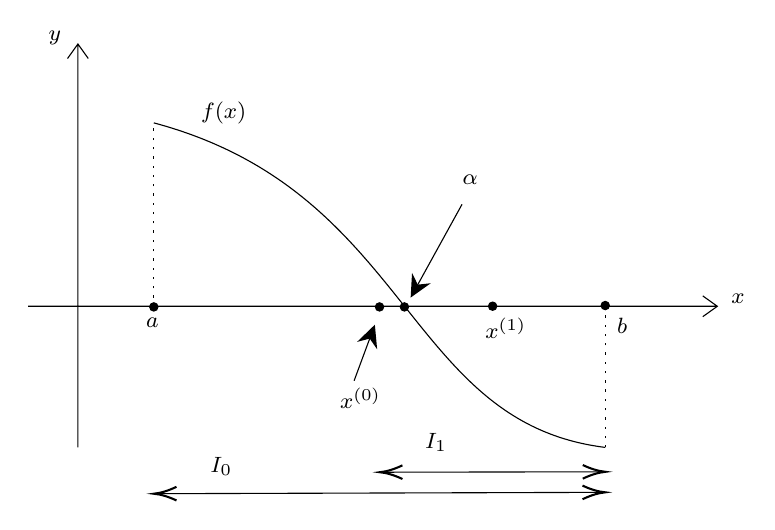
\begin{tikzpicture}[x=0.75pt,y=0.75pt,yscale=-1,xscale=1]
	%uncomment if require: \path (0,253); %set diagram left start at 0, and has height of 253

	%Shape: Axis 2D [id:dp33533961877243534]
	\draw  (133.5,142.36) -- (465.5,142.36)(157.43,16) -- (157.43,210.36) (458.5,137.36) -- (465.5,142.36) -- (458.5,147.36) (152.43,23) -- (157.43,16) -- (162.43,23)  ;
	%Curve Lines [id:da20121558433876752]
	\draw    (194,54) .. controls (318.5,87.34) and (314.5,198.34) .. (411.5,210.36) ;
	%Straight Lines [id:da9661795821517285]
	\draw  [dash pattern={on 0.84pt off 2.51pt}]  (194,142.67) -- (194,54) ;
	%Straight Lines [id:da4873438279286455]
	\draw  [dash pattern={on 0.84pt off 2.51pt}]  (411.5,210.36) -- (411.5,142) ;
	%Straight Lines [id:da9946674756730165]
	\draw    (304.86,222.31) -- (409.61,222.11) ;
	\draw [shift={(411.61,222.11)}, rotate = 539.9] [color={rgb, 255:red, 0; green, 0; blue, 0 }  ][line width=0.75]    (10.93,-3.29) .. controls (6.95,-1.4) and (3.31,-0.3) .. (0,0) .. controls (3.31,0.3) and (6.95,1.4) .. (10.93,3.29)   ;
	\draw [shift={(302.86,222.31)}, rotate = 359.9] [color={rgb, 255:red, 0; green, 0; blue, 0 }  ][line width=0.75]    (10.93,-3.29) .. controls (6.95,-1.4) and (3.31,-0.3) .. (0,0) .. controls (3.31,0.3) and (6.95,1.4) .. (10.93,3.29)   ;
	%Shape: Circle [id:dp8374417825384726]
	\draw  [fill={rgb, 255:red, 0; green, 0; blue, 0 }  ,fill opacity=1 ] (192,142.67) .. controls (192,141.56) and (192.9,140.67) .. (194,140.67) .. controls (195.1,140.67) and (196,141.56) .. (196,142.67) .. controls (196,143.77) and (195.1,144.67) .. (194,144.67) .. controls (192.9,144.67) and (192,143.77) .. (192,142.67) -- cycle ;
	%Shape: Circle [id:dp032665240645063376]
	\draw  [fill={rgb, 255:red, 0; green, 0; blue, 0 }  ,fill opacity=1 ] (300.75,142.67) .. controls (300.75,141.56) and (301.65,140.67) .. (302.75,140.67) .. controls (303.85,140.67) and (304.75,141.56) .. (304.75,142.67) .. controls (304.75,143.77) and (303.85,144.67) .. (302.75,144.67) .. controls (301.65,144.67) and (300.75,143.77) .. (300.75,142.67) -- cycle ;
	%Shape: Circle [id:dp9304288736660509]
	\draw  [fill={rgb, 255:red, 0; green, 0; blue, 0 }  ,fill opacity=1 ] (312.75,142.67) .. controls (312.75,141.56) and (313.65,140.67) .. (314.75,140.67) .. controls (315.85,140.67) and (316.75,141.56) .. (316.75,142.67) .. controls (316.75,143.77) and (315.85,144.67) .. (314.75,144.67) .. controls (313.65,144.67) and (312.75,143.77) .. (312.75,142.67) -- cycle ;
	%Shape: Circle [id:dp9634240894311528]
	\draw  [fill={rgb, 255:red, 0; green, 0; blue, 0 }  ,fill opacity=1 ] (409.5,142) .. controls (409.5,140.9) and (410.4,140) .. (411.5,140) .. controls (412.6,140) and (413.5,140.9) .. (413.5,142) .. controls (413.5,143.1) and (412.6,144) .. (411.5,144) .. controls (410.4,144) and (409.5,143.1) .. (409.5,142) -- cycle ;
	%Shape: Circle [id:dp1350212381008955]
	\draw  [fill={rgb, 255:red, 0; green, 0; blue, 0 }  ,fill opacity=1 ] (355.24,142.33) .. controls (355.24,141.23) and (356.13,140.33) .. (357.24,140.33) .. controls (358.34,140.33) and (359.24,141.23) .. (359.24,142.33) .. controls (359.24,143.44) and (358.34,144.33) .. (357.24,144.33) .. controls (356.13,144.33) and (355.24,143.44) .. (355.24,142.33) -- cycle ;
	%Straight Lines [id:da07104153441328442]
	\draw    (196,232.66) -- (409.5,232.01) ;
	\draw [shift={(411.5,232)}, rotate = 539.8199999999999] [color={rgb, 255:red, 0; green, 0; blue, 0 }  ][line width=0.75]    (10.93,-3.29) .. controls (6.95,-1.4) and (3.31,-0.3) .. (0,0) .. controls (3.31,0.3) and (6.95,1.4) .. (10.93,3.29)   ;
	\draw [shift={(194,232.67)}, rotate = 359.82] [color={rgb, 255:red, 0; green, 0; blue, 0 }  ][line width=0.75]    (10.93,-3.29) .. controls (6.95,-1.4) and (3.31,-0.3) .. (0,0) .. controls (3.31,0.3) and (6.95,1.4) .. (10.93,3.29)   ;
	%Straight Lines [id:da08740253227174466]
	\draw    (342.5,93.25) -- (319.2,135.54) ;
	\draw [shift={(317.75,138.17)}, rotate = 298.86] [fill={rgb, 255:red, 0; green, 0; blue, 0 }  ][line width=0.08]  [draw opacity=0] (10.72,-5.15) -- (0,0) -- (10.72,5.15) -- (7.12,0) -- cycle    ;
	%Straight Lines [id:da9937908466011312]
	\draw    (290.5,178.25) -- (299.46,154.06) ;
	\draw [shift={(300.5,151.25)}, rotate = 470.32] [fill={rgb, 255:red, 0; green, 0; blue, 0 }  ][line width=0.08]  [draw opacity=0] (10.72,-5.15) -- (0,0) -- (10.72,5.15) -- (7.12,0) -- cycle    ;

	% Text Node
	\draw (215.5,42.4) node [anchor=north west][inner sep=0.75pt]  [font=\footnotesize]  {$f(x)$};
	% Text Node
	\draw (471,135.4) node [anchor=north west][inner sep=0.75pt]  [font=\footnotesize]  {$x$};
	% Text Node
	\draw (142,8.4) node [anchor=north west][inner sep=0.75pt]  [font=\footnotesize]  {$y$};
	% Text Node
	\draw (341.5,77.9) node [anchor=north west][inner sep=0.75pt]  [font=\footnotesize]  {$\alpha $};
	% Text Node
	\draw (220,213.9) node [anchor=north west][inner sep=0.75pt]  [font=\footnotesize]  {$I_{0}$};
	% Text Node
	\draw (323.5,202.4) node [anchor=north west][inner sep=0.75pt]  [font=\footnotesize]  {$I_{1}$};
	% Text Node
	\draw (189,146.9) node [anchor=north west][inner sep=0.75pt]  [font=\footnotesize]  {$a$};
	% Text Node
	\draw (416,146.9) node [anchor=north west][inner sep=0.75pt]  [font=\footnotesize]  {$b$};
	% Text Node
	\draw (282.5,180.4) node [anchor=north west][inner sep=0.75pt]  [font=\footnotesize]  {$x^{(0)}$};
	% Text Node
	\draw (352.5,146.9) node [anchor=north west][inner sep=0.75pt]  [font=\footnotesize]  {$x^{(1)}$};
	\end{tikzpicture}
	\caption{L'errore col metodo di bisezione non tende a zero in modo monotono.}
	\label{fig:osservazione-errore-non-monotono}
\end{figure}
\FloatBarrier

In generale, la successione degli errori $e^{(k)}$ generata dal metodo di bisezione non converge a zero \textit{monotonicamente}.
\begin{definition}
[Ordine di convergenza]
\index{ordine!di convergenza}
Sia $\left\{x^{(k)}\right\}_{k\geqslant 0}$ la successione di approssimazioni di $\alpha $ generata da un metodo numerico. Diciamo che la successione converge ad $\alpha $ con ordine $p$, con $\geqslant 1$, se esiste $C >0$ tale che
\begin{equation*}
\frac{\left| x^{( k+1)} -\alpha \right| }{\left| x^{(k)} -\alpha \right| ^{p}} \leqslant C,\quad \forall k\geqslant k_{0} ,\quad k_{0} \in \mathbb{Z}_{+} \cup \{0\} .
\end{equation*}
Se $p=1$, per avere convergenza deve essere $C< 1$, e in questo caso $C$ è detto \textbf{fattore di convergenza}\index{fattore di convergenza}.
\end{definition}
Vogliamo costruire dei metodi numerici che garantiscano convergenza secondo questa definizione.
\section{Approccio geometrico per l'approssimazione di radici}

L'idea è di fare uno sviluppo di Taylor nell'intorno del punto $x$:
\begin{equation*}
0 =f( \alpha ) =f( x+( \alpha -x)) = f(x) +( \alpha -x) f'( \xi ).
\end{equation*}
Se pensiamo la soluzione $\alpha$ come l'iterata successiva $x^{( k+1)}$ e $x$ come il punto nel quale il metodo si trova attualmente, otteniamo la struttura del metodo iterativo:
\begin{equation*}
f\left( x^{(k)}\right) +\left( x^{( k+1)} -x^{(k)}\right) f'( \xi ) =0.
\end{equation*}
Si noti che il punto $\xi $ non è noto, altrimenti basterebbe un solo passo, calcolando la derivata della funzione in $\xi$ e arrivando direttamente ad $\alpha $.
Per questa ragione, sostituiamo il termine $f'( \xi )$ con $q^{(k)}$, la cui scelta caratterizzerà il metodo numerico e determinerà la velocità con cui esso arriverà ad $\alpha $:
\begin{equation*}
\begin{aligned}
f\left( x^{(k)}\right) +\left( x^{( k+1)} -x^{(k)}\right) q^{(k)} & =0\\
\left( x^{( k+1)} -x^{(k)}\right) q^{(k)} & =-f\left( x^{(k)}\right)\\
x^{( k+1)} -x^{(k)} & =-\frac{f\left( x^{(k)}\right)}{q^{(k)}}\\
x^{( k+1)} & =x^{(k)} -\frac{f\left( x^{(k)}\right)}{q^{(k)}}.
\end{aligned}
\end{equation*}
La forma generale è quindi:
\begin{equation}
x^{( k+1)} =x^{(k)} -\frac{1}{q^{(k)}} f\left( x^{(k)}\right) ,\ \ \forall k\geqslant 0.
\label{eq:forma-generale-non-lineari}
\end{equation}

Vediamo ora tre metodi per approssimare le radici:
\begin{itemize}
	\item \textbf{Metodo di Newton}\index{metodo!di Newton}:
		Supponiamo $f\in C^{1}( a,b)$ e $f'(x)\neq 0, \forall x \in (a,b)$, scegliamo
		\begin{equation*}
		q^{(k)} =f'\left( x^{(k)}\right) ,\ \ \forall k\geqslant 0,
		\end{equation*}
		allora \eqref{eq:forma-generale-non-lineari} diventa:
		\begin{equation*}
		x^{( k+1)} =x^{(k)} -\frac{f\left( x^{(k)}\right)}{f'\left( x^{(k)}\right)} ,\ \ \forall k\geqslant 0.
		\end{equation*}
	\item \textbf{Metodo delle secanti}\index{metodo!delle secanti}:
		Per il metodo delle secanti, scegliamo invece
		\begin{equation*}
		q^{(k)} =\frac{f\left( x^{(k)}\right) -f\left( x^{(k-1)}\right)}{x^{(k)} -x^{(k-1)}} ,\ \ \forall k\geqslant 1,
		\end{equation*}
		allora \eqref{eq:forma-generale-non-lineari} diventa:
		\begin{equation*}
		x^{(k+1)} =x^{(k)} -\frac{x^{(k)} -x^{(k-1)}}{f\left( x^{(k)}\right) -f\left( x^{(k-1)}\right)} f\left( x^{(k)}\right) ,\ \ \forall k\geqslant 1.
		\end{equation*}
	\item \textbf{Metodo delle corde}\index{metodo!delle corde}:
		Il metodo delle corde usa:
		\begin{equation*}
		q^{(k)} =q=\frac{f(b)-f(a)}{b-a} ,\ \ \forall k\geqslant 0,
		\end{equation*}
		quindi \eqref{eq:forma-generale-non-lineari} diventa:
		\begin{equation*}
		x^{(k+1)} =x^{(k)} -\frac{b-a}{f(b)-f(a)} f\left( x^{(k)}\right) ,\ \ \forall k\geqslant 0.
		\end{equation*}
\end{itemize}

\textbf{NB.}
I metodi descritti convergono \textit{localmente} rispetto alla definizione che ci siamo dati, ovvero è importante che il dato iniziale $x^{(0)}$ sia scelto ragionevolmente vicino allo zero esatto della funzione. Diversamente dai metodi iterativi per sistemi lineari, qui la scelta del dato iniziale è importante.

\section{Metodo delle iterazioni di punto fisso}
Vediamo un modo più generale di vedere gli algoritmi per equazioni non lineari.
A questo scopo, sia $\alpha $ tale che $f( \alpha ) =0$. Se definiamo:
\begin{equation}
	\Phi ( x) \coloneqq x-f( x) ,
\end{equation}
allora risulta che $\alpha $ è un \textbf{punto fisso}\index{punto fisso} di $\Phi ( x)$, infatti:
\begin{equation*}
	\Phi ( \alpha ) =\alpha -\underbrace{f( \alpha )}_{=0} =\alpha,
\end{equation*}
quindi cercare gli zeri di $f$ è equivalente a cercare i punti fissi della cosiddetta \textbf{funzione di iterazione}\index{funzione!di iterazione} $\Phi ( x)$.

L'idea è di calcolare ogni iterata come la funzione di iterazione valutata all'iterata precedente:
\begin{equation}
	x^{( k+1)} =\Phi \big( x^{(k)}\big) ,\ \ k\geqslant 0,
	\label{eq:iterazioni-punto-fisso}
\end{equation}
e si prosegue fino a convergenza.

L'algoritmo è pertanto il seguente.

\begin{algo}
	inizializza $\x^{(0)}$\;
	\For{$k=0,1,\dotsc$}{
		$x^{(k+1)} = \Phi\left( x^{(k)} \right)$\;
		\If{criterio di arresto}{
			termina algoritmo\;
		}
	}
	\caption{Algoritmo delle iterazioni di punto fisso.}
\end{algo}

L'approccio visivo si può osservare in figura \ref{fig:intuizione-punto-fisso}.

\begin{figure}[htpb]
	\centering
	\tikzset{every picture/.style={line width=0.75pt}} %set default line width to 0.75pt        

	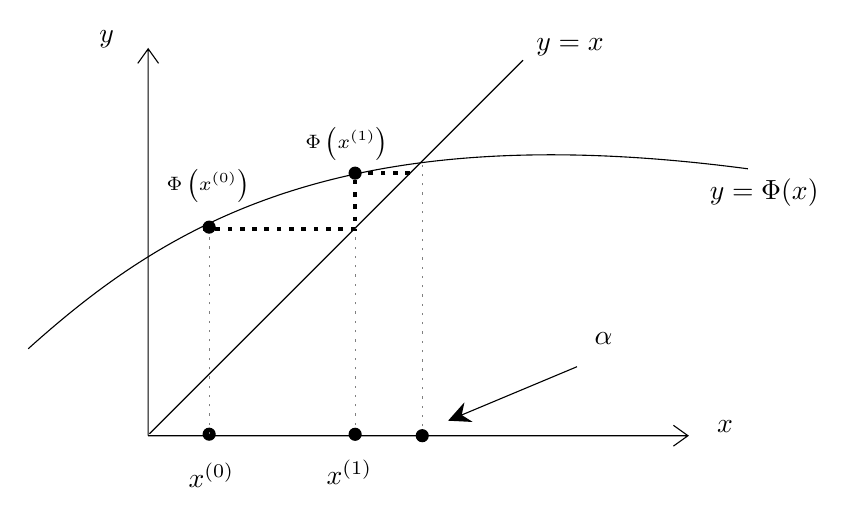
\begin{tikzpicture}[x=0.75pt,y=0.75pt,yscale=-1,xscale=1]
	%uncomment if require: \path (0,300); %set diagram left start at 0, and has height of 300

	%Shape: Axis 2D [id:dp3566775992086928] 
	\draw  (157.79,212.28) -- (417.86,212.28)(157.79,25.89) -- (157.79,212.28) -- cycle (410.86,207.28) -- (417.86,212.28) -- (410.86,217.28) (152.79,32.89) -- (157.79,25.89) -- (162.79,32.89)  ;
	%Curve Lines [id:da6752669888557952] 
	\draw    (100,170.38) .. controls (165.98,111.14) and (250.55,57.68) .. (446.76,83.69) ;
	%Straight Lines [id:da8869587279017774] 
	\draw [color={rgb, 255:red, 128; green, 128; blue, 128 }  ,draw opacity=1 ] [dash pattern={on 0.84pt off 2.51pt}]  (289.83,212.28) -- (289.83,81.24) ;
	%Straight Lines [id:da5511356307086455] 
	\draw [color={rgb, 255:red, 128; green, 128; blue, 128 }  ,draw opacity=1 ] [dash pattern={on 0.84pt off 2.51pt}]  (257.49,211.59) -- (257.49,112.82) ;
	%Shape: Circle [id:dp7693840113711456] 
	\draw  [fill={rgb, 255:red, 0; green, 0; blue, 0 }  ,fill opacity=1 ] (184.28,211.55) .. controls (184.28,209.96) and (185.58,208.66) .. (187.17,208.66) .. controls (188.77,208.66) and (190.06,209.96) .. (190.06,211.55) .. controls (190.06,213.15) and (188.77,214.44) .. (187.17,214.44) .. controls (185.58,214.44) and (184.28,213.15) .. (184.28,211.55) -- cycle ;
	%Shape: Ellipse [id:dp4236145004323377] 
	\draw  [fill={rgb, 255:red, 0; green, 0; blue, 0 }  ,fill opacity=1 ] (286.94,212.28) .. controls (286.94,210.68) and (288.23,209.39) .. (289.83,209.39) .. controls (291.42,209.39) and (292.72,210.68) .. (292.72,212.28) .. controls (292.72,213.87) and (291.42,215.17) .. (289.83,215.17) .. controls (288.23,215.17) and (286.94,213.87) .. (286.94,212.28) -- cycle ;
	%Shape: Ellipse [id:dp6046639245591658] 
	\draw  [fill={rgb, 255:red, 0; green, 0; blue, 0 }  ,fill opacity=1 ] (254.6,211.59) .. controls (254.6,210) and (255.89,208.7) .. (257.49,208.7) .. controls (259.08,208.7) and (260.38,210) .. (260.38,211.59) .. controls (260.38,213.19) and (259.08,214.48) .. (257.49,214.48) .. controls (255.89,214.48) and (254.6,213.19) .. (254.6,211.59) -- cycle ;
	%Straight Lines [id:da5989367722690591] 
	\draw    (364.4,179.04) -- (305.04,203.89) ;
	\draw [shift={(302.28,205.05)}, rotate = 337.28999999999996] [fill={rgb, 255:red, 0; green, 0; blue, 0 }  ][line width=0.08]  [draw opacity=0] (10.72,-5.15) -- (0,0) -- (10.72,5.15) -- (7.12,0) -- cycle    ;
	%Straight Lines [id:da8569096885462997] 
	\draw    (338.4,31.37) -- (158.42,211.35) ;
	%Straight Lines [id:da14498326366026926] 
	\draw [line width=1.5]  [dash pattern={on 1.69pt off 2.76pt}]  (283.97,85.79) -- (257.49,85.79) -- (257.49,112.82) -- (182.36,112.82) ;
	%Straight Lines [id:da6377659143246175] 
	\draw [color={rgb, 255:red, 128; green, 128; blue, 128 }  ,draw opacity=1 ] [dash pattern={on 0.84pt off 2.51pt}]  (187.17,211.55) -- (187.17,111.79) ;
	%Shape: Ellipse [id:dp979569157625213] 
	\draw  [fill={rgb, 255:red, 0; green, 0; blue, 0 }  ,fill opacity=1 ] (184.28,111.79) .. controls (184.28,110.2) and (185.58,108.9) .. (187.17,108.9) .. controls (188.77,108.9) and (190.06,110.2) .. (190.06,111.79) .. controls (190.06,113.39) and (188.77,114.68) .. (187.17,114.68) .. controls (185.58,114.68) and (184.28,113.39) .. (184.28,111.79) -- cycle ;
	%Shape: Ellipse [id:dp09526697663217876] 
	\draw  [fill={rgb, 255:red, 0; green, 0; blue, 0 }  ,fill opacity=1 ] (254.6,85.79) .. controls (254.6,84.19) and (255.89,82.9) .. (257.49,82.9) .. controls (259.08,82.9) and (260.38,84.19) .. (260.38,85.79) .. controls (260.38,87.38) and (259.08,88.68) .. (257.49,88.68) .. controls (255.89,88.68) and (254.6,87.38) .. (254.6,85.79) -- cycle ;

	% Text Node
	\draw (427.1,87.42) node [anchor=north west][inner sep=0.75pt]  [font=\normalsize]  {$y=\Phi ( x)$};
	% Text Node
	\draw (430.64,203.79) node [anchor=north west][inner sep=0.75pt]  [font=\normalsize]  {$x$};
	% Text Node
	\draw (133.01,15.96) node [anchor=north west][inner sep=0.75pt]  [font=\normalsize]  {$y$};
	% Text Node
	\draw (371.63,161.33) node [anchor=north west][inner sep=0.75pt]  [font=\normalsize]  {$\alpha $};
	% Text Node
	\draw (176.04,224.16) node [anchor=north west][inner sep=0.75pt]  [font=\normalsize]  {$x^{( 0)}$};
	% Text Node
	\draw (242.5,222.48) node [anchor=north west][inner sep=0.75pt]  [font=\normalsize]  {$x^{( 1)}$};
	% Text Node
	\draw (343.52,19.51) node [anchor=north west][inner sep=0.75pt]  [font=\normalsize]  {$y=x$};
	% Text Node
	\draw (165.47,82.64) node [anchor=north west][inner sep=0.75pt]  [font=\scriptsize]  {$\Phi \left( x^{( 0)}\right)$};
	% Text Node
	\draw (232.21,62.45) node [anchor=north west][inner sep=0.75pt]  [font=\scriptsize]  {$\Phi \left( x^{( 1)}\right)$};


	\end{tikzpicture}
	\caption{Intuizione geometrica del metodo delle iterazioni di punto fisso.}
	\label{fig:intuizione-punto-fisso}
\end{figure}

È tuttavia facile pensare a dei controesempi in cui la funzione $\Phi $ non porta a convergenza, come in figura \ref{fig:punto-fisso-no-convergenza}. Tale problema sarà risolto nel teorema \ref{thm:ostrowski}.

\begin{figure}[htpb]
	\centering
	

	\tikzset{every picture/.style={line width=0.75pt}} %set default line width to 0.75pt        

	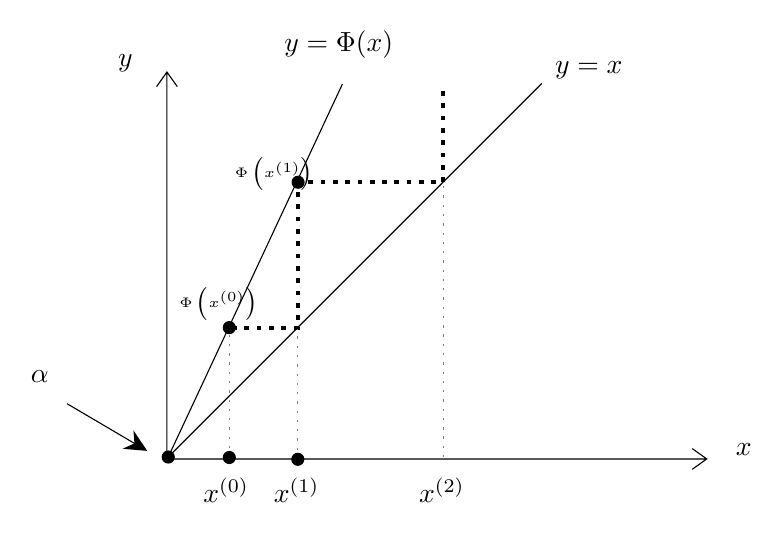
\begin{tikzpicture}[x=0.75pt,y=0.75pt,yscale=-1,xscale=1]
	%uncomment if require: \path (0,300); %set diagram left start at 0, and has height of 300

	%Shape: Axis 2D [id:dp1346140806136602] 
	\draw  (157.79,232.28) -- (417.86,232.28)(157.79,45.89) -- (157.79,232.28) -- cycle (410.86,227.28) -- (417.86,232.28) -- (410.86,237.28) (152.79,52.89) -- (157.79,45.89) -- (162.79,52.89)  ;
	%Straight Lines [id:da5286058801327398] 
	\draw [color={rgb, 255:red, 128; green, 128; blue, 128 }  ,draw opacity=1 ] [dash pattern={on 0.84pt off 2.51pt}]  (290.97,231.5) -- (290.97,98.96) ;
	%Straight Lines [id:da563386105754107] 
	\draw [color={rgb, 255:red, 128; green, 128; blue, 128 }  ,draw opacity=1 ] [dash pattern={on 0.84pt off 2.51pt}]  (187.84,231.59) -- (187.84,169) ;
	%Shape: Ellipse [id:dp6287751568639635] 
	\draw  [fill={rgb, 255:red, 0; green, 0; blue, 0 }  ,fill opacity=1 ] (155.53,231.35) .. controls (155.53,229.75) and (156.82,228.46) .. (158.42,228.46) .. controls (160.01,228.46) and (161.31,229.75) .. (161.31,231.35) .. controls (161.31,232.95) and (160.01,234.24) .. (158.42,234.24) .. controls (156.82,234.24) and (155.53,232.95) .. (155.53,231.35) -- cycle ;
	%Shape: Ellipse [id:dp21716140586002886] 
	\draw  [fill={rgb, 255:red, 0; green, 0; blue, 0 }  ,fill opacity=1 ] (184.95,231.59) .. controls (184.95,230) and (186.24,228.7) .. (187.84,228.7) .. controls (189.43,228.7) and (190.73,230) .. (190.73,231.59) .. controls (190.73,233.19) and (189.43,234.48) .. (187.84,234.48) .. controls (186.24,234.48) and (184.95,233.19) .. (184.95,231.59) -- cycle ;
	%Straight Lines [id:da4765382924209203] 
	\draw    (109.67,205.67) -- (145.69,226.86) ;
	\draw [shift={(148.28,228.39)}, rotate = 210.47] [fill={rgb, 255:red, 0; green, 0; blue, 0 }  ][line width=0.08]  [draw opacity=0] (10.72,-5.15) -- (0,0) -- (10.72,5.15) -- (7.12,0) -- cycle    ;
	%Straight Lines [id:da10658482700916871] 
	\draw    (338.4,51.37) -- (158.42,231.35) ;
	%Straight Lines [id:da1798774361287676] 
	\draw [line width=1.5]  [dash pattern={on 1.69pt off 2.76pt}]  (290.97,55) -- (290.97,98.96) -- (220.97,98.96) -- (220.97,169) -- (187.84,169) ;
	%Straight Lines [id:da4108558993374163] 
	\draw    (242.33,51.67) -- (158.42,231.35) ;
	%Shape: Ellipse [id:dp960624181595366] 
	\draw  [fill={rgb, 255:red, 0; green, 0; blue, 0 }  ,fill opacity=1 ] (184.95,169) .. controls (184.95,167.4) and (186.24,166.11) .. (187.84,166.11) .. controls (189.43,166.11) and (190.73,167.4) .. (190.73,169) .. controls (190.73,170.6) and (189.43,171.89) .. (187.84,171.89) .. controls (186.24,171.89) and (184.95,170.6) .. (184.95,169) -- cycle ;
	%Straight Lines [id:da06469788534794985] 
	\draw [color={rgb, 255:red, 128; green, 128; blue, 128 }  ,draw opacity=1 ] [dash pattern={on 0.84pt off 2.51pt}]  (220.84,232.44) -- (220.84,169.85) ;
	%Shape: Ellipse [id:dp29351931672149534] 
	\draw  [fill={rgb, 255:red, 0; green, 0; blue, 0 }  ,fill opacity=1 ] (217.95,232.44) .. controls (217.95,230.85) and (219.24,229.55) .. (220.84,229.55) .. controls (222.43,229.55) and (223.73,230.85) .. (223.73,232.44) .. controls (223.73,234.04) and (222.43,235.33) .. (220.84,235.33) .. controls (219.24,235.33) and (217.95,234.04) .. (217.95,232.44) -- cycle ;
	%Shape: Ellipse [id:dp30400825590060854] 
	\draw  [fill={rgb, 255:red, 0; green, 0; blue, 0 }  ,fill opacity=1 ] (218.08,98.96) .. controls (218.08,97.37) and (219.37,96.07) .. (220.97,96.07) .. controls (222.56,96.07) and (223.86,97.37) .. (223.86,98.96) .. controls (223.86,100.56) and (222.56,101.85) .. (220.97,101.85) .. controls (219.37,101.85) and (218.08,100.56) .. (218.08,98.96) -- cycle ;

	% Text Node
	\draw (213.1,24.76) node [anchor=north west][inner sep=0.75pt]  [font=\normalsize]  {$y=\Phi ( x)$};
	% Text Node
	\draw (430.64,223.79) node [anchor=north west][inner sep=0.75pt]  [font=\normalsize]  {$x$};
	% Text Node
	\draw (133.01,35.96) node [anchor=north west][inner sep=0.75pt]  [font=\normalsize]  {$y$};
	% Text Node
	\draw (90.96,188.66) node [anchor=north west][inner sep=0.75pt]  [font=\normalsize]  {$\alpha $};
	% Text Node
	\draw (174.04,240.16) node [anchor=north west][inner sep=0.75pt]  [font=\normalsize]  {$x^{( 0)}$};
	% Text Node
	\draw (343.52,39.51) node [anchor=north west][inner sep=0.75pt]  [font=\normalsize]  {$y=x$};
	% Text Node
	\draw (162.47,148.31) node [anchor=north west][inner sep=0.75pt]  [font=\tiny]  {$\Phi \left( x^{( 0)}\right)$};
	% Text Node
	\draw (189.21,85.79) node [anchor=north west][inner sep=0.75pt]  [font=\tiny]  {$\Phi \left( x^{( 1)}\right)$};
	% Text Node
	\draw (208.04,240.16) node [anchor=north west][inner sep=0.75pt]  [font=\normalsize]  {$x^{( 1)}$};
	% Text Node
	\draw (278.04,240.16) node [anchor=north west][inner sep=0.75pt]  [font=\normalsize]  {$x^{( 2)}$};


	\end{tikzpicture}
	\caption{Esempio in cui il metodo di punto fisso non porta a convergenza.}
	\label{fig:punto-fisso-no-convergenza}
\end{figure}

\textit{Osservazione.}
Il metodo delle corde e il metodo di Newton possono essere scritti come metodi di iterazione di punto fisso:
\begin{itemize}
\item Metodo delle corde:
\begin{equation*}
x^{(0)} ,\ \ x^{(k+1)} =\Phi _{\text{corde}}\left( x^{(k)}\right) \quad \text{con } \ \Phi _{\text{corde}}(x) =x-\frac{b-a}{f(b)-f(a)} f(x).
\end{equation*}
\item Metodo di Newton:
\begin{equation*}
x^{(k+1)} =\Phi _{\text{Newton}}\left( x^{(k)}\right) \quad \text{con  } \ \Phi _{\text{Newton}}(x) =x-\frac{f(x)}{f'(x)}.
\end{equation*}
\end{itemize}
\begin{theorem}
[Convergenza delle iterazioni di punto fisso]
\index{teorema!della convergenza delle iterazioni di punto fisso}
Consideriamo la successione delle iterazioni di punto fisso \eqref{eq:iterazioni-punto-fisso}.

Supponiamo che $\Phi $ sia continua in $[ a,b]$ e sia tale che $\Phi (x) \in [ a,b]$ per ogni $x\in [ a,b]$; allora esiste almeno un punto fisso $\alpha \in [ a,b]$.

Se supponiamo inoltre che $\Phi $ sia una contrazione, cioè che:
\begin{equation*}
\exists L< 1\ \text{t.c.} \ | \Phi ( x_{1}) -\Phi ( x_{2})| \leq L| x_{1} -x_{2}| \quad \forall x_{1} ,x_{2} \in [a,b].
\end{equation*}
Allora il punto fisso $\alpha$ è unico e la successione \eqref{eq:iterazioni-punto-fisso} converge ad $\alpha $, per qualunque scelta del dato iniziale $x^{(0)} \in [ a,b]$.
\end{theorem}

\begin{theorem}
[di Ostrowski]
\label{thm:ostrowski}
\index{teorema!di Ostrowski}
Sia $\alpha $ un punto fisso di una funzione $\Phi $ continua e derivabile con continuità in un opportuno intorno $I$ di $\alpha $. Se risulta $| \Phi '(\alpha )| < 1$, allora esiste $\delta  >0$ tale che la successione $\left\{x^{(k)}\right\}$ converge ad $\alpha $, per ogni $x^{(0)}$ per cui si abbia $\left| x^{(0)} -\alpha \right| < \delta $. Inoltre:
\begin{equation*}
\lim _{k\rightarrow \infty }\frac{x^{(k+1)} -\alpha }{x^{(k)} -\alpha } =\Phi '(\alpha ).
\end{equation*}
\end{theorem}
La quantità $| \Phi '(\alpha )| $ è detta \textbf{fattore asintotico di convergenza}\index{fattore!asintotico di convergenza} e, in analogia con il caso dei metodi iterativi per la risoluzione di sistemi lineari, si definisce la \textbf{velocità asintotica di convergenza}\index{velocità!asintotica di convergenza} come segue:
\begin{equation*}
R=-\log(| \Phi '(\alpha )| ).
\end{equation*}
Ricapitolando:
\begin{itemize}
\item se $| \Phi '(\alpha )| < 1$ il metodo è localmente convergente. In particolare:
\begin{itemize}
\item se $\Phi '(\alpha ) >0$ le iterate si avvicinano ad $\alpha $ in maniera monotona;
\item se $\Phi '(\alpha )< 0$ le iterate si avvicinano ad $\alpha $ oscillando intorno ad $\alpha $;
\end{itemize}
\item se $| \Phi '(\alpha )|  >1$ il metodo è divergente;
\item se $| \Phi '(\alpha )| =1$ non è possibile trarre conclusioni dal teorema.
\end{itemize}
Vediamo ora un altro risultato notevole sui metodi di punto fisso.
\begin{theorem}
Se $\Phi \in C^{p+1} (I)$ per un opportuno intorno $I$ di $\alpha $ e per un intero $p\geqslant 1,$ e se $\Phi ^{(i)} (\alpha )=0$ per $i=1,\dotsc ,p$ mentre $\Phi ^{(p+1)} (\alpha )\neq 0,$ allora il metodo di punto fisso con funzione di iterazione $\Phi $ ha ordine $p+1$ e risulta inoltre che
\begin{equation*}
\lim _{k\rightarrow \infty }\frac{x^{(k+1)} -\alpha }{\left( x^{(k)} -\alpha \right)^{p+1}} =\frac{\Phi ^{(p+1)} (\alpha )}{(p+1)!}.
\end{equation*}
\end{theorem}

\subsection{Convergenza del metodo delle corde}
Ricordiamo che per il metodo delle corde si ha che:
\begin{equation*}
\Phi _{\text{corde}}(x) =x-\frac{b-a}{f(b)-f(a)} f(x).
\end{equation*}
Osserviamo che se $f\in C^{1}([ a,b]) $ allora $ \Phi _{\text{corde}} \in C^{1}([ a,b])$. Inoltre:
\begin{equation*}
\Phi '_{\text{corde}}(x) =1-\frac{b-a}{f(b)-f(a)} f'(x).
\end{equation*}
Ora, se $\alpha $ è lo zero di $f$ ($\alpha $ è il punto fisso di $\Phi _{\text{corde}}$), vorremmo usare il teorema di Ostrowski.
Verifichiamo dove esso sia applicabile:
\begin{equation*}
| \Phi '_{\text{corde}}( \alpha )| =\left| 1-\frac{b-a}{f(b)-f(a)} f'( \alpha )\right| =\begin{cases}
\text{se} \ f'( \alpha ) =0\Rightarrow | \Phi '_{\text{corde}}( \alpha )| =1\ \text{(no)}\\
\text{se} \ f'( \alpha ) \neq 0\Rightarrow | \Phi '_{\text{corde}}( \alpha )| < 1\ \text{(sì)}.
\end{cases}
\end{equation*}
Studiamo quindi la disequazione che permette di applicare il teorema:
\begin{gather*}
\left| 1-\frac{b-a}{f(b)-f(a)} f'( \alpha )\right| < 1 \\
\Updownarrow\\
  -1< 1-\frac{b-a}{f(b)-f(a)} f'( \alpha ) < 1\\
 \Updownarrow\\
 \begin{cases}
\displaystyle\frac{b-a}{f(b)-f(a)} f'( \alpha )  >0 \vspace*{1em}\\
\displaystyle\frac{b-a}{f(b)-f(a)} f'( \alpha ) < 2
\end{cases}\\
 \Updownarrow\\
 \begin{cases}
\displaystyle\frac{b-a}{f(b)-f(a)} \ \text{e} \ f'( \alpha ) \ \text{concordi}\vspace*{1em}\\
\displaystyle b-a< \frac{2[ f(b)-f(a)]}{f'( \alpha )}.
\end{cases}
\end{gather*}
Se queste due condizioni sono soddisfatte contemporaneamente, per il teorema di Ostrowski il metodo delle corde converge. Se non dovessero essere soddisfatte, possiamo tentare di fare alcuni passi col metodo di bisezione finché queste condizioni non si verificano.

\subsection{Convergenza del metodo di Newton}
Ricordiamo l'espressione del metodo di Newton:
\begin{equation*}
\Phi _{\text{Newton}}(x) =x-\frac{f(x)}{f'(x)}.
\end{equation*}
Si presentano due casi: o $\alpha $ è uno zero con molteplicità $1$ per $f$ (detto zero semplice), oppure ha molteplicità maggiore di 1.
Affrontiamo questi due casi separatamente.
Supponiamo inizialmente che $\alpha $ sia uno zero semplice, cioè $f( \alpha ) =0$, $f'( \alpha ) \neq 0$. In questo caso:
\begin{equation*}
\Phi '_{\text{Newton}}(x) =1-\frac{[ f'(x)]^{2} -f(x) f''(x)}{[ f'(x)]^{2}}
\end{equation*}
e dunque:
\begin{equation*}
\Phi '_{\text{Newton}}( \alpha ) =1-\frac{[ f'( \alpha )]^{2} -f( \alpha ) f''( \alpha )}{\underbrace{[ f'( \alpha )]^{2}}_{\text{sicuramente} \ \neq 0}} =1-1-\frac{\overbrace{f( \alpha )}^{=0} f''( \alpha )}{[ f'( \alpha )]^{2}} =0.
\end{equation*}
Calcoliamo una derivata successiva per determinare l'ordine di convergenza:
\begin{align*}
\Phi ''_{\text{Newton}}(x) & =\frac{d}{dx}\left[ 1-\frac{[ f']^{2} -ff''}{[ f']^{2}}\right]\\
 & =0-\left(\frac{[ 2f'f''-( f'f''+ff''')]\left[[ f']^{2}\right] -\left[[ f']^{2} -ff''\right][ 2f'f'']}{[ f']^{4}}\right)\\
 & =-\frac{\left[ 2[ f']^{3} f''-[ f']^{3} f''-[ f']^{2} ff'''\right] -\left[ 2[ f']^{3} f''-2ff'[ f'']^{2}\right]}{[ f']^{4}}\\
 & =-\frac{\cancel{2[ f']^{3} f''} -[ f']^{3} f''-[ f']^{2} ff'''\cancel{-2[ f']^{3} f''} +2ff'[ f'']^{2}}{[ f']^{4}}\\
 & =\frac{[ f']^{3} f''+[ f']^{2} ff'''-2ff'[ f'']^{2}}{[ f']^{4}}\\
 & =\frac{[ f']^{2} f''+f'ff'''-2f[ f'']^{2}}{[ f']^{3}}\\
 & =\frac{[ f'(x)]^{2} f''(x) +f(x) f'(x) f'''(x) -2f(x)[ f''(x)]^{2}}{[ f'(x)]^{3}}.
\end{align*}
Pertanto:
\begin{align*}
\Phi ''_{\text{Newton}}( \alpha ) & =\frac{[ f'( \alpha )]^{2} f''( \alpha ) +\overbrace{f( \alpha )}^{=0} f'( \alpha ) f'''( \alpha ) -2\overbrace{f( \alpha )}^{=0}[ f''( \alpha )]^{2}}{[ f'( \alpha )]^{3}}\\
 & =\frac{[ f'( \alpha )]^{2} f''( \alpha )}{[ f'( \alpha )]^{3}}\\
 & =\frac{f''( \alpha )}{f'( \alpha )} \neq 0.
\end{align*}
In questo caso il metodo di Newton converge localmente con ordine $2$.

Supponiamo ora invece che $\alpha $ sia uno zero con molteplicità $m >1$, cioè:
\begin{equation*}
f( \alpha ) =0,\ \ f'( \alpha ) =0,\ \ f''( \alpha ) =0,\ \ \dotsc ,\ \ f^{( m-1)}( \alpha ) =0,\ \ f^{(m)}( \alpha ) \neq 0.
\end{equation*}
In questo caso si può dimostrare che:
\begin{equation*}
\Phi '_{\text{Newton}}( \alpha ) =1-\frac{1}{m} \neq 0,
\end{equation*}
ovvero che il metodo converge localmente con ordine $1$. Abbiamo perso un ordine, ma possiamo ripristinarlo utilizzando il \textbf{metodo di Newton modificato}\index{metodo!di Newton modificato} (NM):
\begin{equation*}
x^{( k+1)} =x^{(k)} -m\frac{f\left( x^{(k)}\right)}{f'\left( x^{(k)}\right)}.
\end{equation*}
In particolare:
\begin{equation*}
\Phi _{\text{NM}}(x) =x-m\frac{f(x)}{f'(x)} \ \ \Rightarrow \ \ \Phi '_{\text{NM}}(x) =1-m\left[\frac{[ f'(x)]^{2} -f(x) f''(x)}{[ f'(x)]^{2}}\right]
\end{equation*}
dove $m$ è la molteplicità di $\alpha$. Ovviamente occorrono dei modi per stimare questa molteplicità, ma essi esulano dall'ambito di questa trattazione.


% \textit{[Lezione 24 (25-05-2020)]}
\section{Criteri di arresto}
%magari iniziare con "In questa sezione, sia ..."
Sia $\left\{x^{(k)}\right\}_{k\geqslant 0}$ la successione di approssimazioni generata da uno dei metodi iterativi illustrati.
Consideriamo l'errore $e^{(k)} =\alpha -x^{(k)} ,\forall k$.
Supponiamo $f\in C^{1}( I_{\alpha })$, con $I_{\alpha }$ intorno di $\alpha $.
\subsection{Controllo del residuo}

Fissiamo una tolleranza $\varepsilon  >0$. Terminiamo il ciclo dell'algoritmo quando
\begin{equation*}
\left| f\left( x^{(k)}\right)\right| \leqslant \varepsilon.
\end{equation*}
In particolare, si può dimostrare che
\begin{enumerate}
\item Se $| f'( \alpha )| \approx 1$ allora $\left| e^{( k)}\right| \approx \varepsilon $ e quindi il \textbf{criterio di arresto è affidabile}\index{criterio di arresto!affidabile}.

\begin{figure}[htpb]
	\centering
	\tikzset{every picture/.style={line width=0.75pt}} %set default line width to 0.75pt

	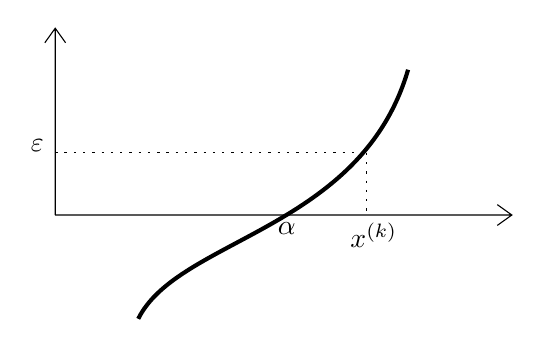
\begin{tikzpicture}[x=0.75pt,y=0.75pt,yscale=-1,xscale=1]
	%uncomment if require: \path (0,160); %set diagram left start at 0, and has height of 160

	%Shape: Axis 2D [id:dp0781238009436287]
	\draw  (170,100) -- (390,100)(170,10) -- (170,100) -- cycle (383,95) -- (390,100) -- (383,105) (165,17) -- (170,10) -- (175,17)  ;
	%Curve Lines [id:da9488325471753964]
	\draw [line width=1.5]    (210,150) .. controls (229.33,111.14) and (317.4,107.4) .. (340,30) ;
	%Straight Lines [id:da7511237307631471]
	\draw  [dash pattern={on 0.84pt off 2.51pt}]  (320,70) -- (320,100) ;
	%Straight Lines [id:da6198333171550376]
	\draw  [dash pattern={on 0.84pt off 2.51pt}]  (170,70) -- (320,70) ;

	% Text Node
	\draw (276,102.4) node [anchor=north west][inner sep=0.75pt]    {$\alpha $};
	% Text Node
	\draw (311,102.4) node [anchor=north west][inner sep=0.75pt]    {$x^{( k)}$};
	% Text Node
	\draw (157,62.4) node [anchor=north west][inner sep=0.75pt]    {$\varepsilon $};


	\end{tikzpicture}
\end{figure}
\FloatBarrier

\item Se $| f'( \alpha )| \ll 1$ allora $\left| e^{( k)}\right| \gg \varepsilon $ e quindi il \textbf{criterio di arresto è inaffidabile}\index{criterio di arresto!inaffidabile}. Si noti in figura come l'errore sia molto piccolo, ma la soluzione sia ancora molto lontana dallo zero.

\begin{figure}[htpb]
	\centering
	\tikzset{every picture/.style={line width=0.75pt}} %set default line width to 0.75pt

	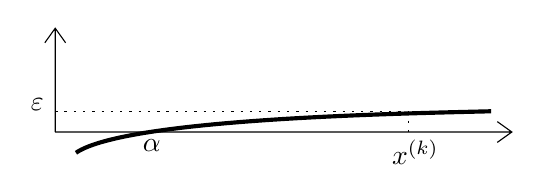
\begin{tikzpicture}[x=0.75pt,y=0.75pt,yscale=-1,xscale=1]
	%uncomment if require: \path (0,99); %set diagram left start at 0, and has height of 99

	%Shape: Axis 2D [id:dp6157046149660421]
	\draw  (180,60) -- (400,60)(180,10) -- (180,60) -- cycle (393,55) -- (400,60) -- (393,65) (175,17) -- (180,10) -- (185,17)  ;
	%Curve Lines [id:da6682504735242709]
	\draw [line width=1.5]    (190,70) .. controls (215,53) and (353.67,51) .. (390,50) ;
	%Straight Lines [id:da3642195964671542]
	\draw  [dash pattern={on 0.84pt off 2.51pt}]  (350,50) -- (350,60) ;
	%Straight Lines [id:da11427175041099624]
	\draw  [dash pattern={on 0.84pt off 2.51pt}]  (180,50) -- (350,50) ;

	% Text Node
	\draw (221,62.4) node [anchor=north west][inner sep=0.75pt]    {$\alpha $};
	% Text Node
	\draw (341,62.4) node [anchor=north west][inner sep=0.75pt]    {$x^{( k)}$};
	% Text Node
	\draw (167,42.4) node [anchor=north west][inner sep=0.75pt]    {$\varepsilon $};


	\end{tikzpicture}
\end{figure}
\FloatBarrier

\item Se $| f'( \alpha )| \gg 1$ allora $\left| e^{( k)}\right| \ll \varepsilon $ e quindi il \textbf{criterio di arresto è troppo stringente}\index{criterio di arresto!troppo stringente}. Si noti in figura il contrario rispetto al punto precedente: l'errore è molto grande anche se la soluzione è molto vicina.

\begin{figure}[htpb]
	\centering
	\tikzset{every picture/.style={line width=0.75pt}} %set default line width to 0.75pt

	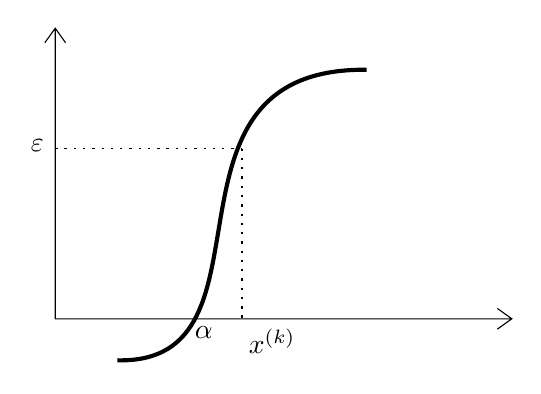
\begin{tikzpicture}[x=0.75pt,y=0.75pt,yscale=-1,xscale=1]
	%uncomment if require: \path (0,201); %set diagram left start at 0, and has height of 201

	%Shape: Axis 2D [id:dp16565494826021832]
	\draw  (180,160) -- (400,160)(180,20) -- (180,160) -- cycle (393,155) -- (400,160) -- (393,165) (175,27) -- (180,20) -- (185,27)  ;
	%Curve Lines [id:da0007870013764332828]
	\draw [line width=1.5]    (210,180) .. controls (292,181.84) and (221,38.84) .. (330,40) ;
	%Straight Lines [id:da25268726559402355]
	\draw  [dash pattern={on 0.84pt off 2.51pt}]  (270,78) -- (270,160) ;
	%Straight Lines [id:da28261351997743933]
	\draw  [dash pattern={on 0.84pt off 2.51pt}]  (180,78) -- (270,78) ;

	% Text Node
	\draw (246,162.4) node [anchor=north west][inner sep=0.75pt]    {$\alpha $};
	% Text Node
	\draw (272,163.4) node [anchor=north west][inner sep=0.75pt]    {$x^{( k)}$};
	% Text Node
	\draw (167,72.4) node [anchor=north west][inner sep=0.75pt]    {$\varepsilon $};


	\end{tikzpicture}
\end{figure}
\FloatBarrier

\end{enumerate}

\subsection{Controllo sull'incremento}
Fissando la tolleranza $\varepsilon  >0$, terminiamo il ciclo quando
\begin{equation*}
\left| x^{( k+1)} -x^{(k)}\right| < \varepsilon.
\end{equation*}
Grazie a uno sviluppo di Taylor possiamo scrivere
\begin{equation*}
e^{( k+1)} =\alpha -x^{( k+1)} =\Phi ( \alpha ) -\Phi \left( x^{( k)}\right) =\Phi '\left( \xi ^{( k)}\right) e^{( k)}
\end{equation*}
allora
\begin{equation*}
x^{( k+1)} -x^{( k)} =e^{( k)} -e^{( k+1)} =\left( 1-\Phi '\left( \xi ^{( k)}\right)\right) e^{( k)}.
\end{equation*}
Dato che $\xi ^{( k)}$ sta convergendo ad $\alpha $ possiamo assumere che $\Phi '\left( \xi ^{( k)}\right) \approx \Phi '( \alpha )$, da cui
\begin{equation}
e^{( k)} =\frac{1}{1-\Phi '( \alpha )}\left( x^{( k+1)} -x^{( k)}\right).
\end{equation}
Quindi:
\begin{itemize}
\item se $\Phi '( \alpha ) \approx 1$ allora il criterio è \textit{inaffidabile};
\item per i metodi del secondo ordine, se $\Phi '( \alpha ) =0$ allora il criterio è \textit{affidabile};
\item continua ad essere soddisfacente se $-1< \Phi '( \alpha ) < 0$.
\end{itemize}

\section{Sistemi di equazioni non lineari}
Vediamo l'estensione vettoriale dello stesso tipo di problema visto nelle pagine precedenti.
Sia assegnata $\mathbf{F} :\mathbb{R}^{n}\rightarrow \mathbb{R}^{n}$: vogliamo trovare $\x^{\star } \in \mathbb{R}^{n}$ tale che $\mathbf{F}\left(\x^{\star }\right) =\mathbf{0}$.

Ricordiamo che la \textbf{matrice jacobiana}\index{matrice!jacobiana} associata a $\mathbf{F}$ e valutata nel punto $\x =( x_{1} ,x_{2} ,\dotsc ,x_{n})^{T}$ è data da:
\begin{equation*}
( J_{\mathbf{F}}(\x))_{ij} =\frac{\partial F_{i}}{\partial x_{j}}(\x) ,\quad i,j=1,\dotsc ,n.
\end{equation*}

Supponiamo anche che $\mathbf{F}$ sia una funzione continua e con derivate parziali positive.
Si ha il seguente algoritmo di punto fisso:

\begin{algo}
	inizializza $\x^{(0)}$\;
	\For{$k=0,1,2,\dotsc$}{
		risolvi $J_{\mathbf{F}}\left(\x^{(k)}\right) \delta \x^{(k)} =-\mathbf{F}\left( x^{(k)}\right)$\;
		aggiorna $\x^{( k+1)} =\x^{(k)} +\delta \x^{(k)}$\;
		\If{criterio di arresto}{
			termina algoritmo\;
		}
	}
	\caption{Algoritmo di Newton per sistemi non lineari.}
\end{algo}
\textit{Osservazione.} Esistono molte varianti di questo algoritmo, ad esempio basate su opportune approssimazioni di $J_{\mathbf{F}}\left(\x^{(k)}\right)$ oppure sull'aggiornamento di $J_{\mathbf{F}}\left(\x^{(k)}\right)$ solo una volta ogni $k^*$ iterazioni, con $k^* > 1$.
\begin{theorem}
[Convergenza di Newton per sistemi non lineari]
Sia $\mathbf{F} :\mathbb{R}^{n}\rightarrow \mathbb{R}^{n}$, $\mathbf{F} \in C^{1}(D)$, dove $D$ è un sottoinsieme aperto convesso di $\mathbb{R}^{n}$ che contiene $\x^{\star }$. Supponiamo inoltre che $J_{\mathbf{F}}\left(\x^{\star }\right)$ sia invertibile, e che esistano delle costanti positive $R,C,L$ tali che $\left\Vert J^{-1}_{\mathbf{F}}\left(\x^{\star }\right)\right\Vert \leqslant C$ e
\begin{equation*}
\Vert J_{\mathbf{F}}(\mathbf{z}) -J_{\mathbf{F}}(\y)\Vert \leqslant L\Vert \mathbf{z} -\y\Vert ,\quad \forall \mathbf{z} ,\y \in B\left(\x^{\star } ,R\right)
\end{equation*}
avendo indicato con lo stesso simbolo $\Vert \cdot \Vert $ una norma vettoriale ed una norma matriciale consistenti\footnote{Una norma matriciale $\Vert \cdot \Vert $ su $\mathbb{R}^{m\times n}$ è consistente con una norma vettoriale $\Vert \cdot \Vert _{a}$ su $\mathbb{R}^{n}$ e $\Vert \cdot \Vert _{b}$ su $\mathbb{R}^{m}$ se $\Vert A\x\Vert _{b} \leqslant \Vert A\Vert \Vert \x\Vert _{a}$ per tutte le matrici $A\in \mathbb{R}^{m\times n}$ e i vettori $\x \in \mathbb{R}^{n}$. Tutte le norme indotte, cioè quelle che consideriamo in questo corso, sono consistenti per definizione.}.
Esiste allora $r >0$ tale che, per ogni $\x^{(0)} \in B\left(\x^{\star } ,r\right)$ il metodo di Newton è univocamente definito, converge a $\x^{\star }$ ed è tale che
\begin{equation*}
\left\Vert \x^{(k+1)} -\x^{\star }\right\Vert \leq CL\left\Vert \x^{(k)} -\x^{\star }\right\Vert ^{2}.
\end{equation*}
\end{theorem}

\appendix
%!TEX root = ../main.tex
\chapter{Richiami di algebra lineare}

Il testo richiede la conoscenza di basilari concetti dall'algebra lineare.
In questa appendice presentiamo alcuni utili richiami alla materia.

\section{Vettori e spazi vettoriali}

\begin{definition}
	[Spazio vettoriale]
	\index{Spazio vettoriale}
	Chiamiamo spazio vettoriale $V$ su un campo $K$, solitamente con $K=\mathbb{R}$, un insieme non vuoto i cui elementi, detti vettori, sono dotati di un operatore di addizione $+:V\times V\rightarrow V$ e un operatore di moltiplicazione per scalare $\cdot :K\times V\rightarrow V$.
  Questi operatori devono possedere le seguenti proprietà, per ogni scelta dei vettori $\mathbf{a}, \mathbf{b}, \mathbf{c}, \mathbf{v}, \mathbf{w} \in V$ coinvolti:
\begin{itemize}
	\item l'addizione è associativa, ovvero $\mathbf{a} +(\mathbf{b} +\mathbf{c}) =(\mathbf{a} +\mathbf{b}) +\mathbf{c}$, e commutativa, cioè $\mathbf{a} +\mathbf{b} =\mathbf{b} +\mathbf{a}$;
	\item esiste un vettore nullo $\mathbf{0} \in V$ tale che $\mathbf{v} +\mathbf{0} =\mathbf{v}$;
	\item $0\cdot \mathbf{v} =\mathbf{0}$ e $1\cdot \mathbf{v} =\mathbf{v}$;
	\item per ogni elemento $\mathbf{v}$ di $V$ esiste ed appartiene a $V$ il suo opposto $( -\mathbf{v})$, ovvero che sia tale che $\mathbf{v} + ( -\mathbf{v}) = \mathbf{0}$;
	\item vale la proprietà distributiva, ovvero $( \alpha +\beta )\mathbf{v} =\alpha \mathbf{v} +\beta \mathbf{v}$ e $\alpha (\mathbf{v} +\mathbf{w}) =\alpha \mathbf{v} +\alpha \mathbf{w}$ per ogni scelta degli scalari $\alpha ,\beta \in K$.
\end{itemize}
\end{definition}
Notiamo che queste proprietà sono simili a quelle possedute dai numeri scalari con cui normalmente si opera.

I vettori sono quindi \textit{rappresentabili} come $n$-uple ordinate di numeri. Ai fini di questo corso è utile vederli proprio come \textit{colonne}, denotate da:
\begin{equation*}
\mathbf{v} =\begin{bmatrix}
v_{1}\\
v_{2}\\
\vdots \\
v_{n}
\end{bmatrix} ,\ \ \mathbf{v} \in V.
\end{equation*}
\begin{definition}
	Un insieme di vettori $\{\mathbf{v}_{1} ,\dotsc ,\mathbf{v}_{n}\}$ si dice linearmente indipendente se vale la seguente implicazione, con $\alpha _{1} ,\dotsc ,\alpha _{n} \in K$:
	\begin{equation*}
		\alpha _{1}\mathbf{v}_{1} +\dotsc +\alpha _{n}\mathbf{v}_{n} =\mathbf{0} \ \ \Rightarrow \ \ \alpha _{1} ,\dotsc ,\alpha _{n} =0.
	\end{equation*}
\end{definition}
\begin{definition}
[Span]
\index{span}
Dato $V$ uno spazio vettoriale su $K$ e un insieme di vettori di $V$: $\{\mathbf{v}_{1} ,\mathbf{v}_{2} ,\dotsc ,\mathbf{v}_{n}\}$, si dice \textit{span} o \textit{spazio generato da vettori} l'insieme di tutte le loro possibili combinazioni lineari, e si indica con:
\begin{equation*}
\text{span}(\mathbf{v}_{1} ,\mathbf{v}_{2} ,\dotsc ,\mathbf{v}_{n}) \coloneqq \left\{a_{1}\mathbf{v}_{1} +a_{2}\mathbf{v}_{2} +\dotsc +a_{n}\mathbf{v}_{n} \ \text{con} \ a_{1} ,a_{2} ,\dotsc ,a_{n} \in K\right\} .
\end{equation*}
\end{definition}
Per esempio, si può facilmente mostrare che i vettori $[1,0]$ e $[2,0]$, che sono elementi di $\mathbb{R}^{2}$, generano $\mathbb{R}$, essendo linearmente \textit{dipendenti}. Invece, i vettori $[2,0]$ e $[4,5]$ generano $\mathbb{R}^{2}$, in quanto sono linearmente \textit{indipendenti}.
\begin{definition}
	[Prodotto scalare]
	\index{prodotto scalare}
	Dato uno spazio vettoriale $V$ su $\mathbb{R}$, un \textit{prodotto scalare} in $V$ è un operatore binario $( \cdot ,\cdot ) :V\times V\rightarrow \mathbb{R} $ tale che, per ogni $\mathbf{v} ,\mathbf{w} ,\x \in V$ e per ogni $\alpha ,\beta \in \mathbb{R} $:
\begin{itemize}
	\item $( \alpha \mathbf{v} +\beta \mathbf{w} ,\x) =\alpha (\mathbf{v} ,\x) +\beta (\mathbf{w} ,\x)$, cioè si ha \textit{linearità} in entrambi gli operandi;
	\item $(\x ,\x) \geqslant 0$;
	\item $(\x ,\x) =0$ se e solo se $\x =\mathbf{0}$.
\end{itemize}
\end{definition}
\begin{definition}
[Prodotto scalare canonico in $\mathbb{R}^{n}$] Tra i vari prodotti scalari possibili per $\mathbb{R}^{n}$, quello definito \textit{canonico} è il prodotto scalare euclideo.
Esso è un operatore binario denotato dal simbolo ``$\, \cdot \,$'', e definito su $\mathbb{R}^{n} \times \mathbb{R}^{n}\rightarrow \mathbb{R}$ nel seguente modo:
\begin{equation*}
\mathbf{u} \cdot \mathbf{v} \coloneqq u_{1} v_{1} +u_{2} v_{2} +\dotsc +u_{n} v_{n}.
\end{equation*}
\end{definition}
Nel seguito quando ci riferiremo al prodotto scalare in $\mathbb{R}^{n}$ indicheremo sempre quello canonico.
\begin{definition}
	[Ortogonalità]
	\index{ortogonalità}
	Due vettori $\x ,\y \in \mathbb{R}^{n}$ sono ortogonali se
	$$(\x ,\y) =0.$$
\end{definition}
\begin{definition}
	[Norma euclidea]
	\index{norma!euclidea}
	Si dice norma euclidea di un vettore $\x \in \mathbb{R}^{n}$ l'operatore $\Vert \cdot \Vert_{2}  :\mathbb{R}^{n}\rightarrow \mathbb{R}$ tale che:
	\begin{equation*}
		\Vert \x\Vert_{2} \coloneqq \sqrt{x^{2}_{1} +x^{2}_{2} +\dotsc +x^{2}_{n}}.
	\end{equation*}
	\label{def:norma-euclidea}
\end{definition}
\begin{definition}
	[Norma indotta]
	\index{norma!indotta}
	Dato un prodotto scalare $( \cdot ,\cdot )$, la norma indotta da tale prodotto scalare è definita come:
	\begin{equation*}
		\Vert \x\Vert \coloneqq \sqrt{(\x ,\x)}.
	\end{equation*}
  Essa rispetta tutte le proprietà richieste ad un operatore norma.
\end{definition}
Per esempio, la norma euclidea è la norma indotta dal prodotto scalare canonico in $\mathbb{R}^{n}$:
\begin{equation*}
  \Vert \x\Vert_{2} =\sqrt{\x \cdot \x}.
\end{equation*}

\section{Matrici}
\begin{definition}
	[Matrice]
	\index{matrice}
	Una matrice $A$ di dimensioni $m\times n$ sul campo $K$ è una tabella di $mn$ elementi di $K$.
  I suoi elementi saranno indicati con la notazione $( a_{ij})$, dove $i$ è l'indice della riga dell'elemento e $j$ quello della sua colonna, con $1\leqslant i\leqslant m$ e $1\leqslant j\leqslant n$.
  Una matrice si rappresenta nel seguente modo:
	\begin{equation*}
		A=\begin{bmatrix}
		a_{11} & a_{12} & \cdots  & a_{1n}\\
		a_{21} & a_{22} & \cdots  & a_{2n}\\
		\vdots  & \vdots  & \ddots  & \vdots \\
		a_{m1} & a_{m2} & \cdots  & a_{mn}
		\end{bmatrix}
	\end{equation*}
	Per indicare una matrice su $\mathbb{R}$ di $m$ righe e $n$ colonne si dirà $A\in \mathbb{R}^{m\times n}$.
\end{definition}


\begin{definition}
[Prodotto tra matrici]
\index{prodotto tra matrici}
Date due matrici $A\in \mathbb{R}^{m\times p}$ e $B\in \mathbb{R}^{p\times n}$ (inclusi i casi in cui $m, n$ e/o $p$ siano uguali a 1), si dice prodotto righe per colonne, o semplicemente prodotto tra le due matrici, la matrice $C\in \mathbb{R}^{m\times n}$ definita per componenti da:
\begin{equation*}
c_{ik} =\sum _{j=1}^{p} a_{ij} b_{jk} ,\ \ \forall i=1,\dotsc ,m,\ \forall k=1,\dotsc ,n.
\end{equation*}
In altre parole, la componente $ik$ del risultato è il prodotto scalare canonico della riga $i$ di $A$ e della colonna $k$ di $B$.
\end{definition}
Evidenziamo che il numero $p$ di colonne di $A$ e di righe di $B$ devono essere uguali. \\
La definizione è ancora valida se una o entrambe le matrici coinvolte sono in realtà vettori (``orizzontali'' oppure ``verticali''), i quali possono essere visti come casi particolari di matrici con una dimensione unitaria. \\
\textit{Esempio.} Consideriamo:
\begin{equation*}
A=\begin{bmatrix}
a & b\\
c & d
\end{bmatrix} \quad B=\begin{bmatrix}
x & y & z\\
u & v & w
\end{bmatrix} ,
\end{equation*}
il loro prodotto è
\begin{equation*}
AB=\begin{bmatrix}
ax+bu & ay+bv & az+bw\\
cx+du & cy+dv & cz+dw
\end{bmatrix} .
\end{equation*}
Osserviamo che in generale $AB\neq BA$, infatti:
\begin{equation*}
A=\begin{bmatrix}
0 & 0\\
0 & 1
\end{bmatrix} \quad B=\begin{bmatrix}
0 & 0\\
1 & 0
\end{bmatrix} \ \ \Rightarrow \ \ AB=\begin{bmatrix}
0 & 0\\
1 & 0
\end{bmatrix} \neq \begin{bmatrix}
0 & 0\\
0 & 0
\end{bmatrix} =BA.
\end{equation*}
Presentiamo ora una serie di comuni classificazioni per le matrici.
\begin{definition}
	[Matrice quadrata]
	\index{matrice!quadrata}
	Una matrice $m\times n$ si dice \textit{quadrata} se $m=n$, cioè se il numero di righe è uguale al numero di colonne.
\end{definition}
\begin{definition}
	[Matrice invertibile]
	\index{matrice!invertibile}
	Data una matrice quadrata, si dice \textit{invertibile} se esiste una matrice $B$ con lo stesso numero di righe e colonne tale che:
	\begin{equation*}
		BA=AB=I,
	\end{equation*}
	dove $I$ è la \textit{matrice identità}, delle stesse dimensioni, costruita come $( I)_{ij} =\delta _{ij}$, cioè $1$ se $i=j$ e $0$ se $i\neq j$. La matrice inversa di $A$ si indica con la notazione $A^{-1}$.
\end{definition}
\begin{definition}
	[Matrice trasposta]
	\index{matrice!trasposta}
	Data una matrice $A\in \mathbb{R}^{m\times n}$, si definisce la sua \textit{matrice trasposta} la matrice $B\in \mathbb{R}^{n\times m}$ tale che $b_{ij} = a_{ji}$ per ogni indice $i,j$, ovvero ottenuta ``ruotando'' la matrice scambiando righe e colonne ma mantenendone l'ordine.
\end{definition}
È facile dimostrare le seguenti proprietà della trasposta:
\begin{gather*}
	\left( A^{T}\right)^{T} =A,\quad ( A+B)^{T} =A^{T} +B^{T} ,\\
	( AB)^{T} =B^{T} A^{T} ,\quad ( \alpha A)^{T} =\alpha A^{T}.
\end{gather*}
Inoltre, se $A$ è invertibile si ha:
\begin{equation*}
	\left( A^{T}\right)^{-1} =\left( A^{-1}\right)^{T} \eqqcolon A^{-T}.
\end{equation*}
\begin{definition}
	Data una matrice quadrata $A\in \mathbb{R}^{n\times n}$:
\begin{itemize}
	\item essa è \textbf{simmetrica}\index{matrice!simmetrica} se $A=A^{T}$, cioè se $a_{ij} =a_{ji}$ per ogni $i,j=1,\dotsc ,n$;
	\item essa è \textbf{diagonale}\index{matrice!diagonale} se $a_{ij} =0$ per ogni $i\neq j$.
  La \textit{matrice identità} è quindi un caso particolare di matrice diagonale;
	\item essa è \textbf{triangolare superiore}\index{matrice!triangolare} (risp. \textbf{inferiore}) se $a_{ij} =0$ per ogni $i >j$ (risp. $i< j$).
\end{itemize}
\end{definition}

\textit{Esempi.}
Ecco alcuni esempi delle tipologie di matrici appena presentate:
\begin{itemize}
\item simmetrica,\begin{equation*}
\begin{bmatrix}
3 & 2 & 17 & 34\\
2 & 5 & 1 & 8\\
17 & 1 & 9 & e\\
34 & 8 & e & 22
\end{bmatrix}
\end{equation*}
\item diagonale,\begin{equation*}
\begin{bmatrix}
13 & 0 & 0 & 0\\
0 & \pi  & 0 & 0\\
0 & 0 & 4 & 0\\
0 & 0 & 0 & 9
\end{bmatrix}
\end{equation*}
\item triangolare superiore,\begin{equation*}
\begin{bmatrix}
1 & 4 & 0 & 11\\
0 & 29 & 2 & 15\\
0 & 0 & 6 & 7\\
0 & 0 & 0 & 5
\end{bmatrix}
\end{equation*}
\item triangolare inferiore.\begin{equation*}
\begin{bmatrix}
5 & 0 & 0 & 0\\
7 & 14 & 0 & 0\\
0 & 8 & 80 & 0\\
4 & \pi  & 9 & 66
\end{bmatrix}
\end{equation*}
\end{itemize}

Le matrici quadrate hanno due grandezze scalari fondamentali ad esse associate: il determinante e la traccia.
\begin{definition}
	[Determinante]
	\index{determinante}
	Data una matrice quadrata $A\in \mathbb{R}^{n\times n}$, si definisce \textit{determinante} di $A$ la seguente quantità scalare:
	\begin{equation*}
		\operatorname{det} A \coloneqq \sum\limits _{\sigma \in S_{n}}\sgn( \sigma ) a_{1\sigma ( 1)} \dotsc a_{n\sigma ( n)} ,
	\end{equation*}
	dove $S_{n}$ indica l'insieme delle $n!$ permutazioni di $\{1,\dotsc ,n\}$, e $\sgn( \sigma )$ indica il segno della permutazione, cioè $1$ (risp. $-1$) se il numero di scambi con cui si ottiene è pari (risp. dispari).
\end{definition}

\begin{theorem}
	[Sviluppo di Laplace]
	\index{sviluppo di Laplace}
	Consideriamo una matrice quadrata $A\in \mathbb{R}^{n\times n}$ e una sua sottomatrice $C_{ij} \in \mathbb{R}^{( n-1) \times ( n-1)}$ ottenuta rimuovendo la $i$-esima riga e la $j$-esima colonna.
  Allora:
	\begin{equation*}
		\operatorname{det} A=\sum ^{n}_{j=1}( -1)^{i+j} a_{ij}\operatorname{det}( C_{ij}) .
	\end{equation*}
\end{theorem}
Nel caso molto comune di $n=2$ il determinante si trova come:
\begin{equation*}
A=\begin{bmatrix}
a_{11} & a_{12}\\
a_{21} & a_{22}
\end{bmatrix} \quad \operatorname{det}( A) =a_{11} a_{22} -a_{12} a_{21}
\end{equation*}
\begin{theorem}
	Date $A,B\in \mathbb{R}^{n\times n}$, valgono le seguenti proprietà:
	\begin{gather*}
		\operatorname{det}( AB) =\operatorname{det}( A)\operatorname{det}( B) ,\ \ \operatorname{det}\left( A^{-1}\right) =\frac{1}{\operatorname{det}( A)} ,\\
		\operatorname{det}( A) =\operatorname{det}\left( A^{T}\right) ,\ \ \operatorname{det}( \alpha A) =\alpha ^{n}\operatorname{det}( A) ,\ \ \forall \alpha \in K.
	\end{gather*}
  La prima proprietà è nota come teorema di Binet.
\end{theorem}
\begin{definition}
	[Traccia]
	\index{traccia}
	Si definisce \textit{traccia} di una matrice quadrata $A\in \mathbb{R}^{n\times n}$ la somma degli elementi sulla diagonale:
	\begin{equation*}
		\operatorname{tr}( A) \coloneqq \sum ^{n}_{i=1} a_{ii} .
	\end{equation*}
\end{definition}

Esistono, infine, diversi spazi vettoriali associati ad una matrice.
\begin{definition}
	[Rango]
	\index{rango}
	Si dice \textit{rango} (in inglese \textit{rank}) di una matrice $A$ la dimensione dello spazio generato dalle sue colonne.
  Esso viene indicato con $\operatorname{Rank}( A)$.
\end{definition}
Si può dimostrare che si ottiene lo stesso spazio se si usa lo spazio generato dalle righe invece che dalle colonne.
\begin{definition}
	[Nucleo e immagine]
	\index{nucleo}
	\index{kernel}
	\index{immagine}
	Data una matrice $A \in \mathbb{R}^{n \times n}$, si dice \textit{nucleo} o \textit{kernel} di $A$ il seguente spazio:
	\begin{equation*}
		\operatorname{Ker}( A) \coloneqq \left\{\x \in \mathbb{R}^{n} :A\x =\mathbf{0}\right\}
	\end{equation*}
  e \textit{immagine} di $A$ il seguente spazio:
  \begin{equation*}
    \operatorname{Im}( A) \coloneqq \left\{A\x :\x \in \mathbb{R}^{n}\right\} .
  \end{equation*}
\end{definition}
\begin{theorem}
	Valgono le seguenti proprietà:
	\begin{gather*}
		\operatorname{Rank}( A) =\operatorname{Rank}\left( A^{T}\right) ,\ \ \operatorname{Rank}( A) =\operatorname{dim}(\operatorname{Im}( A)) ,\\
		\operatorname{dim}(\operatorname{Im}( A)) +\operatorname{dim}(\operatorname{Ker}( A)) =n.
	\end{gather*}
  $\operatorname{dim}(\operatorname{Ker}( A))$ viene anche detta \textit{nullità} della matrice.
  L'ultima proprietà porta pertanto il nome di teorema di \textbf{nullità più rango}\index{nullità più rango}.
\end{theorem}
\begin{theorem}
	Data $A\in \mathbb{R}^{n\times n}$, le seguenti affermazioni sono equivalenti:
\begin{itemize}
	\item $A$ è invertibile;
	\item $\operatorname{det}( A) \neq 0$;
	\item $\operatorname{Ker}( A) =\{\mathbf{0}\}$;
	\item $\operatorname{Rank}( A) =n$;
	\item Le righe (e le colonne) di $A$ sono linearmente indipendenti.
\end{itemize}
\end{theorem}

\subsection{Autovalori e autovettori}
Le matrici quadrate posseggono un insieme di valori scalari particolarmente interessanti per l'analisi numerica, gli autovalori, e dei vettori ad essi associati, gli autovettori.

\begin{definition}
	[Autovalore e autovettore]
	\index{autovalore}
	\index{autovettore}
	Consideriamo una matrice $A\in \mathbb{R}^{n\times n}$.
  Si dicono \textit{autovalori} quei $\lambda \in \mathbb{R}$ tali che
	\begin{equation*}
		A\x =\lambda \x ,\ \ \x \in \mathbb{R}^{n}.
	\end{equation*}
	L'insieme degli autovalori è chiamato \textbf{spettro}\index{spettro} di $A$, indicato con $\sigma ( A)$.

	È facile verificare che gli autovalori di una matrice $A$ possono essere determinati calcolando le radici del suo \textbf{polinomio caratteristico}\index{polinomio!caratteristico}:
	\begin{equation*}
		p_{A}( \lambda ) =\operatorname{det}( A-\lambda I) =0.
	\end{equation*}
	Questo è al più un polinomio di grado $n$, per cui vi saranno al massimo $n$ autovalori distinti.
  Inoltre gli $\x$ che soddisfano $A\x =\lambda \x$ si dicono \textit{autovettori}.
\end{definition}
\begin{theorem}
	Una matrice $A\in \mathbb{R}^{n\times n}$ e la sua trasposta hanno gli stessi autovalori.
\end{theorem}
\begin{theorem}
	Gli autovalori di qualsiasi matrice quadrata $A$ sono legati al suo determinante e traccia nel seguente modo:
	\begin{equation*}
		\operatorname{det}( A) =\prod ^{n}_{i=1} \lambda _{i} ,\ \ \operatorname{tr}( A) =\sum ^{n}_{i=1} \lambda _{i} .
	\end{equation*}
\end{theorem}
\begin{definition}
	[Matrice definita positiva/negativa]
	\index{matrice!definita positiva}
	\index{matrice!definita negativa}
	Una matrice quadrata $A\in \mathbb{R} ^{n\times n} $ si dice definita positiva (risp. negativa) se $\x^{T} A\x > 0$ (risp. $< 0$) per ogni $\x \neq \mathbf{0}$, $\x \in \mathbb{R}^{n}$.
	\label{def:matrice-definita-positiva-negativa}
\end{definition}
\begin{theorem}
	Sia $A$ una matrice quadrata di dimensione $n$.
  Le seguenti affermazioni sono equivalenti:
	\begin{itemize}
		\item $A$ è \textit{definita positiva} (\textit{negativa});
		\item tutti gli autovalori di $A$ sono positivi (negativi);
		\item \textbf{Criterio di Sylvester}\index{criterio!di Sylvester}: tutti i minori di Nord-Ovest\footnote{I determinanti delle sottomatrici di ordine $k$ ottenute eliminando le ultime $( n-k)$ righe e colonne, con $0\leqslant k\leqslant n-1$.} sono positivi (tutti i minori di Nord-Ovest di ordine dispari sono negativi e i minori di testa di ordine pari sono positivi).
	\end{itemize}
	\label{thm:matrice-definita-positiva-negativa}
\end{theorem}
\begin{definition}
	Due matrici $A,B$ sono \textbf{simili}\index{matrice!simile} se esiste una matrice $P$ invertibile, detta di passaggio, tale che:
	\begin{equation*}
		P^{-1} AP=B.
	\end{equation*}
\end{definition}
\begin{definition}
	Una matrice $A$ è \textbf{diagonalizzabile}\index{matrice!diagonalizzabile} se è simile ad una matrice diagonale, cioè se esiste $P$ invertibile tale che:
	\begin{equation*}
		P^{-1} AP=\Delta ,
	\end{equation*}
	con $\Delta $ matrice diagonale.
\end{definition}
\begin{theorem}
	Una matrice quadrata di dimensione $n$ è diagonalizzabile se e solo se ammette $n$ autovettori linearmente indipendenti.
  Inoltre, una matrice reale simmetrica è sempre diagonalizzabile.
\end{theorem}

\begin{definition}
	[Matrice ortogonale]
	\index{matrice!ortogonale}
	Una matrice $U\in \mathbb{R}^{n\times n}$ è \textit{ortogonale} se:
	\begin{equation*}
		U^{T} U=I=UU^{T} .
	\end{equation*}
\end{definition}
\begin{theorem}
	Se $U\in \mathbb{R}^{n\times n}$ è una matrice quadrata ortogonale, allora:
\begin{itemize}
	\item $\operatorname{det}( U) =\pm 1$;
	\item conseguentemente, $U$ è invertibile, e in particolare $U^{-1} =U^{T}$;
	\item $U^{T}$ è ortogonale;
	\item preserva il prodotto scalare canonico, nel senso che $( U\x ,U\y) =(\x ,\y)$, con $\x ,\y \in \mathbb{R}$.
		Infatti $( U\x ,U\y) =\left(\x ,U^{T} U\y\right) =(\x ,\y)$;
	\item preserva anche la norma euclidea $\Vert U\x\Vert _{2} =\Vert \x\Vert _{2}$.
		Infatti $\Vert U\x\Vert ^{2}_{2} =( U\x ,U\x) =(\x ,\x) =\Vert \x\Vert _{2}^{2} $.
\end{itemize}
\end{theorem}

\listofalgorithms
\printindex
\cleardoublepage

\end{document}
